% !TEX program = pdflatex
% !TEX root = main.tex
%
% Build (from the project root):   latexmk
% Clean:                           latexmk -C
%
% Document class: sapthesis v5.1 (the degree type is derived from \course{...}, not from an option).
% Remove "english" if the thesis is written in Italian (and load babel italian).
\documentclass[english, oneside]{sapthesis}

% ---------------------------------------------------------------------------
% Encoding, language, typography
% NOTE: sapthesis already loads xkeyval, etoolbox, geometry, fontenc, textcomp, lmodern,
% caption, graphicx, color, booktabs, amsmath, fancyhdr. Do not load them again.
% ---------------------------------------------------------------------------
\usepackage[utf8]{inputenc}
\usepackage{microtype}
\usepackage{csquotes}          % required by biblatex for proper quoting
\usepackage{tikz}
\usepackage{subcaption}

% ---------------------------------------------------------------------------
% Math, figures, tables, code
% ---------------------------------------------------------------------------
\usepackage{amssymb}                 % amsmath, graphicx, booktabs, fontenc, lmodern, caption are loaded by sapthesis
\graphicspath{{assets/plots/}{assets/icons/}}   % relative to the project root
\usepackage{tabularx}
\usepackage{placeins}        % \FloatBarrier: keep figures inside their own section
\usepackage{siunitx}           % units and number formatting: \SI{8}{\giga\byte}
\usepackage{subcaption}        % subfigures
\usepackage{xcolor}
\usepackage{tikz}
\usetikzlibrary{arrows.meta, positioning, calc, fit, backgrounds, decorations.pathreplacing}
\usepackage{pgfplots}
\pgfplotsset{compat=1.18}
\usepackage{listings}          % source excerpts from NCCL
\lstset{
  basicstyle=\ttfamily\small,
  columns=fullflexible,
  breaklines=true,
  numbers=left,
  numberstyle=\tiny,
  frame=single,
  captionpos=b,
}

% ---------------------------------------------------------------------------
% Bibliography (biblatex + biber)
% ---------------------------------------------------------------------------
\usepackage[
  backend=biber,
  style=numeric,
  sorting=nyt,
  maxbibnames=10,
]{biblatex}
\addbibresource{src/references.bib}

% ---------------------------------------------------------------------------
% Links and cross-references (load hyperref late, cleveref after it)
% ---------------------------------------------------------------------------
\usepackage[hidelinks]{hyperref}   % print-friendly; see sapthesis doc for colors
\usepackage[nameinlink,capitalise]{cleveref}

% ---------------------------------------------------------------------------
% Acronyms
% ---------------------------------------------------------------------------
\usepackage[printonlyused]{acronym}

% ---------------------------------------------------------------------------
% Project macros (keep notation consistent across chapters)
% ---------------------------------------------------------------------------
\newcommand{\bigO}[1]{\mathcal{O}\!\left(#1\right)}
\newcommand{\nccl}{\textsc{NCCL}}
\newcommand{\bine}{\textsc{Bine}}
\newcommand{\pat}{\textsc{PAT}}
\newcommand{\todo}[1]{\textcolor{red}{[TODO: #1]}}   % remove before submission


\usepackage{amsmath,amssymb,amsthm,booktabs,algorithm,algpseudocode}
\newtheorem{lemma}{Lemma}
\newcommand{\rtn}{\mathit{rank2nb}}
\newcommand{\ntr}{\mathit{nb2rank}}
\newcommand{\nbr}[1]{\overline{#1}}
\newcommand{\Send}{\mathcal{S}}
\newcommand{\Recv}{\mathcal{R}}
\newcommand{\none}{\bot}

\definecolor{crosslink}{RGB}{200,40,40}
\definecolor{localxfer}{RGB}{60,150,70}

\definecolor{chunkA}{RGB}{60,170,70}   % chunk 1 (green)
\definecolor{chunkB}{RGB}{240,200,40}  % chunk 2 (yellow)
\definecolor{chunkC}{RGB}{50,110,220}  % chunk 3 (blue)
\colorlet{idle}{gray!35}

% \ringpic{label}{color 0->1}{color 1->2}{color 2->0}
\newcommand{\ringpic}[4]{%
  \begin{tikzpicture}[baseline=(lab.north),
      rank/.style={circle, draw, minimum size=0.65cm, inner sep=0pt, fill=white},
      lnk/.style={-{Stealth[length=2.5mm]}, line width=2.2pt,
                  shorten >=1pt, shorten <=1pt}]
    \node[rank] (r0) at (90:1.1)   {0};
    \node[rank] (r1) at (-30:1.1)  {1};
    \node[rank] (r2) at (210:1.1)  {2};
    \draw[lnk, #2] (r0) -- (r1);
    \draw[lnk, #3] (r1) -- (r2);
    \draw[lnk, #4] (r2) -- (r0);
    \node (lab) at (0,-1.9) {#1};
  \end{tikzpicture}%
}

% \ftstep{holders}{transfers a/b}{uplink loads j/label}: one step of a broadcast on
% 8 ranks, 4 leaf switches and 1 spine (2:1 oversubscribed fat tree). Each transfer is
% drawn along the links it uses: green if it stays under one leaf switch, red if it
% crosses the uplinks. Ranks in {holders} already have the data; the load of each used
% uplink is written next to it.
\newcommand{\ftstep}[3]{%
  \begin{tikzpicture}[x=0.56cm, y=0.66cm,
      rank/.style={circle, draw, minimum size=0.4cm, inner sep=0pt,
                   fill=white, font=\scriptsize},
      sw/.style={rectangle, rounded corners=1.5pt, draw=black!60, fill=black!8,
                 minimum width=0.62cm, minimum height=0.3cm, inner sep=0pt},
      wire/.style={draw=black!25, line width=0.6pt},
      uplink/.style={draw=black!25, line width=1.6pt},
      path/.style={line width=1.5pt, line join=round, line cap=round},
      load/.style={font=\scriptsize\bfseries, crosslink, inner sep=1pt, fill=white}]
    \foreach \i in {0,...,7} \coordinate (r\i) at (\i,0);
    \foreach \j in {0,...,3} \coordinate (l\j) at (2*\j+0.5,1.6);
    \coordinate (sp) at (3.5,3.3);
    % idle links
    \foreach \i in {0,...,7} {\pgfmathtruncatemacro{\j}{\i/2}\draw[wire] (r\i) -- (l\j);}
    \foreach \j in {0,...,3} \draw[uplink] (l\j) -- (sp);
    % transfers, drawn along the links they use
    \foreach \a/\b in {#2} {
      \pgfmathtruncatemacro{\ja}{\a/2}
      \pgfmathtruncatemacro{\jb}{\b/2}
      \ifnum\ja=\jb
        \draw[path, localxfer, -{Stealth[length=1.8mm]}] (r\a) -- (l\ja) -- ([yshift=0.2cm]r\b);
      \else
        \draw[path, crosslink, -{Stealth[length=1.8mm]}] (r\a) -- (l\ja) -- (sp) -- (l\jb) -- ([yshift=0.2cm]r\b);
      \fi
    }
    % switches and ranks on top of the paths
    \foreach \j in {0,...,3} \node[sw] at (l\j) {};
    \node[sw, minimum width=1.2cm] at (sp) {};
    \foreach \i in {0,...,7} \node[rank] at (r\i) {\i};
    \foreach \h in {#1} \node[rank, fill=black!20] at (r\h) {\h};
    % uplink loads
    \foreach \j/\lab in {#3} \node[load] at ($(l\j)!0.42!(sp)$) {\lab};
  \end{tikzpicture}%
}

% \binepic{label}{active edges}: 8-rank distance-halving Bine tree rooted at 0.
% Tree from the XOR rule q = nb2rank(rank2nb(r) xor 1..1):
%   step 0: 0->3 | step 1: 0->7, 3->4 | step 2: 0->1, 3->2, 7->6, 4->5
\newcommand{\binepic}[2]{%
  \begin{tikzpicture}[baseline=(lab.north), x=0.85cm, y=0.75cm,
      rank/.style={circle, draw, minimum size=0.55cm, inner sep=0pt,
                   fill=white, font=\scriptsize},
      idl/.style={draw=idle, line width=1.2pt},
      act/.style={-{Stealth[length=2.4mm]}, line width=2.2pt,
                  shorten >=1pt, shorten <=1pt},
      mid/.style={-{Stealth[length=2mm]}, line width=1.2pt,
                  shorten >=1pt, shorten <=1pt},
      side/.style={line width=1.2pt, shorten >=1pt, shorten <=1pt}]
    \useasboundingbox (-1.8,0.5) rectangle (2.7,-4.5);
    \node[rank] (n0) at (0.7,0)     {0};
    \node[rank] (n3) at (-0.6,-1.1) {3};
    \node[rank] (n7) at (0.9,-1.1)  {7};
    \node[rank] (n1) at (2.1,-1.1)  {1};
    \node[rank] (n4) at (-1.3,-2.2) {4};
    \node[rank] (n2) at (-0.1,-2.2) {2};
    \node[rank] (n6) at (0.9,-2.2)  {6};
    \node[rank] (n5) at (-1.3,-3.3) {5};
    \foreach \a/\b in {0/3,0/7,0/1,3/4,3/2,7/6,4/5} \draw[idl] (n\a) -- (n\b);
    #2
    \node[font=\footnotesize, align=center] (lab) at (0.45,-4.1) {#1};
  \end{tikzpicture}%
}

% \bact{from}{to}{colour}: one chunk on a link
\newcommand{\bact}[3]{\draw[act, #3] (n#1) -- (n#2);}

% \bslice{from}{to}: the whole slice (all three chunks) on a link
\newcommand{\bslice}[2]{%
  \draw[side, chunkA, transform canvas={xshift=-2.4pt}] (n#1) -- (n#2);
  \draw[side, chunkC, transform canvas={xshift=2.4pt}]  (n#1) -- (n#2);
  \draw[mid, chunkB] (n#1) -- (n#2);}

% \bcastrow{chunk letter}{colour}{first time slot}: one row of the broadcast figure
\newcommand{\bcastrow}[3]{%
  \binepic{chunk #1, step 0\\$t{=}#3$}{\bact{0}{3}{#2}}\hfill
  \binepic{chunk #1, step 1\\$t{=}\the\numexpr#3+1\relax$}%
    {\bact{0}{7}{#2}\bact{3}{4}{#2}}\hfill
  \binepic{chunk #1, step 2\\$t{=}\the\numexpr#3+2\relax$}%
    {\bact{0}{1}{#2}\bact{3}{2}{#2}\bact{7}{6}{#2}\bact{4}{5}{#2}}}

% \blab{from}{to}{slot}{colour}: link used at a given time slot
\newcommand{\blab}[4]{%
  \draw[act, #4] (n#1) -- node[pos=0.55, fill=white, inner sep=0.6pt,
      font=\tiny\bfseries] {#3} (n#2);}

% \bchunk{letter}{slots before this chunk}{colour}: whole tree of one chunk
\newcommand{\bchunk}[3]{%
  \binepic{chunk #1\\slots \the\numexpr#2+1\relax--\the\numexpr#2+3\relax}{%
    \blab{0}{3}{\the\numexpr#2+1\relax}{#3}%
    \blab{0}{7}{\the\numexpr#2+2\relax}{#3}%
    \blab{3}{4}{\the\numexpr#2+2\relax}{#3}%
    \blab{0}{1}{\the\numexpr#2+3\relax}{#3}%
    \blab{3}{2}{\the\numexpr#2+3\relax}{#3}%
    \blab{7}{6}{\the\numexpr#2+3\relax}{#3}%
    \blab{4}{5}{\the\numexpr#2+3\relax}{#3}}}

% Preamble (colors; the tikz libraries arrows.meta, positioning, fit, backgrounds, calc are already loaded)
\definecolor{ch0}{RGB}{60,130,210}
\definecolor{ch1}{RGB}{225,120,50}
\definecolor{ch2}{HTML}{27AE60}


% ---------------------------------------------------------------------------
% Metadata (fill in)
% ---------------------------------------------------------------------------
\title{Implementation of Bine Tree Algorithms\\in NCCL for Multi-GPU Systems}
\author{Daniele Savino}
\IDnumber{2140356}
\course{Laurea in Informatica}        % official ITALIAN course name, even if the thesis is in English
\courseorganizer{Facoltà di Ingegneria dell'Informazione,\\Informatica e Statistica}
\AcademicYear{2025/2026}
\advisor{Prof. Daniele De Sensi}     % the "relatore"
\authoremail{savino.2140356@studenti.uniroma1.it}
\website{https://github.com/DanieleSavino}
\copyyear{2027}
\thesistype{Bachelor thesis}

\hypersetup{
  pdftitle  = {Implementation of Bine Tree Algorithms in NCCL for Multi-GPU Systems},
  pdfauthor = {Daniele Savino},
}

\begin{document}

% ---------------------------------------------------------------------------
% Front matter
% ---------------------------------------------------------------------------
\frontmatter
\maketitle
% \dedication{...}   % optional, recommended by sapthesis instead of long acknowledgements
\begin{abstract}
The cost of a collective operation on a multi-GPU system is increasingly set not by the number of communication steps but by how much traffic crosses the slow, oversubscribed links between nodes.
\bine{} (binomial negabinary) trees are a recently proposed family of collective algorithms that keep the logarithmic step count of binomial trees and butterflies while choosing partners that minimise this distance, cutting the traffic on the slow links by up to a third on several supercomputer networks~\cite{desensi2025bine}.
The original algorithms were implemented and evaluated only at the MPI level, on CPU clusters; this thesis brings them inside \nccl{}, the library most multi-GPU deep learning frameworks rely on for collective communication on NVIDIA GPUs.

The implementation has four components.
A tree-based broadcast and reduce replace \nccl{}'s native ring and double binary tree with the \bine{} tree.
A butterfly-based allgather and reduce-scatter handle, with four buffer-management strategies, the non-contiguous data that \nccl{}'s fixed, per-channel partition of the work imposes on an algorithm whose window of active ranks grows and shrinks at every step.
The same allgather is rebuilt a second time on \pat{}, \nccl{}'s own device-side machinery for aggregating many small transfers into fewer, larger messages.
Finally, a tree-based allreduce, a composition not described in the original \bine{} paper but one that maps well onto \nccl{}'s channel system, roots a \bine{} tree differently on each channel, one root per channel instead of one per rank, and executes the reduce and the broadcast as a single fused kernel following the structure of \nccl{}'s own tree allreduce.

Each component is evaluated on up to 128 GPUs across two supercomputers, against \nccl{}'s native ring, tree and \pat{} algorithms.
The tree-based broadcast and reduce are up to $6.5\times$ faster than the ring at $128$ ranks, in the range of sizes between the ring's latency-optimised and its bandwidth-bound regimes.
The tree-based allreduce is the fastest algorithm overall from $16$ ranks on for vectors up to $1$\,MB, up to $1.39\times$ faster than the best native algorithm at the same size.
The allgather rebuilt on \pat{}, instead, does not improve on the butterfly kernels when several GPUs share a node, and is competitive with \nccl{}'s own \pat{} allgather only when there is one GPU per node.
Taken together, the results give a precise account of where, inside \nccl{}, the locality of \bine{} pays for itself, and where \nccl{}'s own bandwidth-oriented algorithms remain the better choice.
\end{abstract}

% Meluxina, Leonardo
\tableofcontents
\listoffigures
\listoftables
\listofalgorithms   % the algorithms are numbered and cross-referenced like the other floats
\chapter*{Acronyms}
\addcontentsline{toc}{chapter}{Acronyms}
\begin{acronym}[NCCL]
  \acro{CPU}{Central Processing Unit}
  \acro{CUDA}{Compute Unified Device Architecture}
  \acro{FIFO}{First In, First Out}
  \acro{GPU}{Graphics Processing Unit}
  \acro{LL}{Low Latency (\nccl{} protocol)}
  \acro{MPI}{Message Passing Interface}
  \acro{NCCL}{NVIDIA Collective Communications Library}
  \acro{NIC}{Network Interface Card}
  \acro{PAT}{Parallel Aggregated Trees}
  \acro{XOR}{Exclusive OR}
\end{acronym}


% ---------------------------------------------------------------------------
% Main matter
% ---------------------------------------------------------------------------
\mainmatter

% Related work is written last (it "comes naturally"). The abstract stands in
% for a separate introduction chapter.
% Requires: booktabs, amsmath, tikz (arrows.meta), subcaption
\chapter{Background and Related Work}\label{ch:background}

This chapter introduces collective operations and the algorithms that the rest of the thesis builds on.
It describes the ring, the standard binomial tree and the double binary tree used by \nccl{}, which are the baselines of the thesis, the butterfly, and the \bine{} tree~\cite{desensi2025bine}, which is the algorithm implemented in \nccl{} in the following chapters.
The notation introduced here is used throughout the thesis.

%==============================================================================
\section{Collective communication}\label{sec:bg-collectives}

A \emph{collective operation} is executed by all the $p$ processes (\emph{ranks}) of a communicator, each identified by a rank identifier $r\in[0,p-1]$.
The operations considered in this thesis are the following.
\begin{description}
  \item[Broadcast.] The root $t$ holds a vector of $n$ bytes, and every rank must end up with a copy of it.
  \item[Reduce.] Every rank holds a vector of $n$ bytes, and the root $t$ must obtain their element-wise combination (e.g., the sum).
  \item[Scatter and gather.] In a scatter, the root holds $p$ blocks and rank $r$ must receive the $r$-th one. The gather is the opposite operation: the root collects one block from every rank.
  \item[Allgather.] Every rank holds one block, and every rank must obtain the concatenation of all the blocks.
  \item[Reduce-scatter.] Every rank holds a vector of $n$ bytes divided in $p$ blocks, and rank $r$ must obtain the $r$-th block of the element-wise combination of all the vectors.
  \item[Allreduce.] Like the reduce, but every rank obtains the result.
\end{description}
The combination operator is assumed to be associative and commutative, as it is for the operators supported by \nccl{} (sum, product, maximum, minimum, average).
Several collectives are related: the allreduce can be obtained as a reduce-scatter followed by an allgather or as a Reduce followed by a Broadcast, and the broadcast as a scatter followed by an allgather.

\paragraph{Cost model.}
To compare algorithms we use the usual latency--bandwidth model~\cite{hockney1994communication,thakur2005optimization}.
Sending a message of $m$ bytes between two ranks takes $\alpha+m\beta$, where $\alpha$ is the latency (including transmission setup overhead) and $\beta$ the time to transfer one byte, i.e., $\mathrm{bandwidth} = 1/\beta$.
Let $\gamma$ be the cost of aggregating (reducing) two bytes, i.e., the time to apply the reduction operator to one byte from each of two operands. Reducing two vectors of $m$ bytes locally therefore takes $m\gamma$.
Algorithms proceed in \emph{steps}, and at each step a rank sends at most one message and receives at most one.
The model ignores the topology of the network: all the pairs of ranks are assumed to be at the same distance.
This is precisely the assumption that the \bine{} tree relaxes (\cref{sec:bg-bine}).
\cref{tab:notation} summarises the notation we will see all throughout this thesis.

\begin{table}[t]
\centering
\small
\caption{Notation used in the thesis.}
\label{tab:notation}
\begin{tabularx}{\linewidth}{@{}lX@{}}
\toprule
Symbol & Definition \\
\midrule
$p$ & Number of ranks. \\
$r$ & Rank identifier, $r\in[0,p-1]$. \\
$t$ & Rank identifier of the root of the collective. \\
$n$ & Size of the vector of the collective, in bytes. \\
$k$ & Number of chunks in which the vector is split for pipelining. \\
$d$ & Depth of a tree (edges from the root to the deepest leaf), with $d=s$ for the trees of this chapter. \\
$s$ & Number of steps of a tree algorithm, $s=\log_2 p$ ($p$ a power of two). \\
$\alpha,\beta,\gamma$ & Latency, time per byte transferred, time per byte reduced. \\
$\oplus$ & Bitwise exclusive or (XOR). \\
$\rtn(r)$ & Negabinary representation of the rank $r$ (\cref{sec:bg-bine}). \\
$\ntr(x)$ & Rank identifier whose negabinary representation is $x$. \\
\bottomrule
\end{tabularx}
\end{table}

%==============================================================================
\section{Ring, tree and butterfly-style algorithms}\label{sec:bg-algorithms}

Most collective algorithms are built from a small number of communication patterns.
This section describes the three families relevant for this thesis, the ring, the binomial tree and the butterfly, and then the \bine{} variants of the tree and of the butterfly.
Throughout, $p=2^s$ unless stated otherwise.

%------------------------------------------------------------------------------
\subsection{Ring}\label{sec:bg-ring}

In a ring algorithm the ranks are arranged in a logical ring, and at every step rank $r$ sends to rank $(r+1)\bmod p$ and receives from rank $(r-1)\bmod p$ (\cref{fig:bg-ring}).
Each rank talks to only two peers, and all the ranks send and receive at every step.

\begin{figure}[H]
  \centering
  \begin{tikzpicture}[
      rank/.style={circle,draw,minimum size=6.5mm,inner sep=0pt,font=\small},
      >={Stealth[length=2mm]}]
    \foreach \r in {0,...,7}{
      \node[rank] (r\r) at ({90-45*\r}:1.5) {\r};
    }
    \foreach \r/\q in {0/1,1/2,2/3,3/4,4/5,5/6,6/7,7/0}{
      \draw[->,thick] (r\r) -- (r\q);
    }
  \end{tikzpicture}
  \caption{Communication pattern of a ring over $p=8$ ranks. At every step, rank $r$ sends to rank $(r+1)\bmod p$.}
  \label{fig:bg-ring}
\end{figure}

\paragraph{Allgather, reduce-scatter and allreduce.}
In the ring allgather, the vector is divided in $p$ blocks of $n/p$ bytes.
At the first step each rank sends its own block, and at each following step it forwards the block received at the previous one, so that after $p-1$ steps every rank has all the blocks.
The reduce-scatter is the same pattern in which the block received at each step is combined with the local one before being forwarded.
The allreduce is a reduce-scatter followed by an allgather.
The costs are
\begin{align}
  T_{\text{allgather}} &= (p-1)\,\alpha + \tfrac{p-1}{p}\,n\beta,\\
  T_{\text{reduce-scatter}} &= (p-1)\,\alpha + \tfrac{p-1}{p}\,n\beta + \tfrac{p-1}{p}\,n\gamma,\\
  T_{\text{allreduce}} &= 2(p-1)\,\alpha + 2\tfrac{p-1}{p}\,n\beta + \tfrac{p-1}{p}\,n\gamma.
\end{align}
The bandwidth term is optimal: every rank sends and receives a number of bytes that does not grow with $p$ and that matches the lower bound for these collectives.

\paragraph{Broadcast and reduce.}
The ring can also be used for the broadcast and the reduce by pipelining.
The vector is split in $k$ chunks that travel along the ring starting from the root: after the first chunk has reached the last rank, a new chunk is delivered at every step.
\cref{fig:bg-ring-links} illustrates the difference in link usage on a ring of $p=3$ ranks: without pipelining (\cref{fig:bg-ring-nopipe}) the whole vector hops from rank to rank and only one link is busy per step, whereas with pipelining (\cref{fig:bg-ring-pipe}) the chunks follow each other and all links transfer data concurrently.
The broadcast takes $p+k-2$ steps of $n/k$ bytes each,
\begin{equation}
  T_{\text{broadcast}} = (p+k-2)\Bigl(\alpha+\tfrac{n}{k}\beta\Bigr),
  \label{eq:bg-ring-bcast}
\end{equation}
and the reduce is the same pattern in the opposite direction, with an additional $\tfrac{n}{k}\gamma$ per step.
For a large $k$ the bandwidth term tends to $n\beta$, independently of $p$, but the latency term grows linearly with the number of ranks, and chunks cannot be made arbitrarily small without paying $\alpha$ for each of them.

\begin{figure}[H]
  \centering
  \begin{subfigure}[b]{\linewidth}
    \centering
    \ringpic{step 1}{chunkA}{idle}{idle}\hfill
    \ringpic{step 2}{idle}{chunkA}{idle}\hfill
    \ringpic{step 3}{idle}{idle}{chunkA}
    \caption{Without pipelining: the whole vector hops from rank to rank,
             so only one link is busy per step.}
    \label{fig:bg-ring-nopipe}
  \end{subfigure}

  \vspace{1.5em}

  \begin{subfigure}[b]{\linewidth}
    \centering
    \ringpic{step 1}{chunkA}{chunkB}{chunkC}\hfill
    \ringpic{step 2}{chunkC}{chunkA}{chunkB}\hfill
    \ringpic{step 3}{chunkB}{chunkC}{chunkA}
    \caption{With pipelining: the vector is split in three chunks (green, yellow,
             blue) that follow each other, so all links are busy at every step.}
    \label{fig:bg-ring-pipe}
  \end{subfigure}
  \caption{Link usage on a ring of $p=3$ ranks. Arrows are links coloured by the
           chunk they carry, and grey links are idle.}
  \label{fig:bg-ring-links}
\end{figure}

\paragraph{Locality.}
Since each rank communicates only with its two neighbours, a ring whose ranks are mapped consecutively on the machine uses very few long-distance links.
For example, on a network organised in groups, only two of the $p$ messages sent at each step cross a group boundary for every boundary~\cite{desensi2025bine} (\cref{fig:bg-ring-locality}).
This is why the ring is competitive for large vectors even on oversubscribed networks.
Its weakness is the number of steps: the performance is suboptimal for large numbers of ranks and small to medium vectors~\cite{desensi2025bine}, where the latency term $\bigO{p}\,\alpha$ dominates.

\begin{figure}[H]
  \centering
  \begin{tikzpicture}[
      rank/.style={circle, draw, minimum size=0.6cm, inner sep=0pt, fill=white,
                   font=\footnotesize},
      lnk/.style={-{Stealth[length=2mm]}, line width=1.6pt,
                  shorten >=1pt, shorten <=1pt},
      local/.style={lnk, gray!60},
      cross/.style={lnk, crosslink},
      group/.style={rounded corners=3pt, draw=black!60, fill=black!5,
                    inner sep=6pt}]
    % ranks, mapped consecutively
    \foreach \i/\x in {0/0, 1/1.1, 2/2.2, 3/3.3, 4/5.3, 5/6.4, 6/7.5, 7/8.6}
      \node[rank] (r\i) at (\x,0) {\i};

    % groups
    \begin{scope}[on background layer]
      \node[group, fit=(r0)(r3), label={[font=\footnotesize]above:Group A}] (gA) {};
      \node[group, fit=(r4)(r7), label={[font=\footnotesize]above:Group B}] (gB) {};
    \end{scope}

    % links inside a group
    \foreach \i/\j in {0/1, 1/2, 2/3, 4/5, 5/6, 6/7}
      \draw[local] (r\i) -- (r\j);

    % links crossing a group boundary
    \draw[cross] (r3) -- (r4);
    \draw[cross] (r7.south) -- ++(0,-1.1) -| (r0.south);
  \end{tikzpicture}
  \caption{Ring with ranks mapped consecutively on a network organised in two groups.
           Grey links stay inside a group. Only the links between the endpoints of
           the groups (red) cross a group boundary.}
  \label{fig:bg-ring-locality}
\end{figure}

%------------------------------------------------------------------------------
\subsection{Binomial tree}\label{sec:bg-tree}

Here, \emph{tree} always means the standard binomial tree, not the double binary tree used by \nccl{}, which is described in \cref{sec:bg-double-tree}.

\paragraph{Construction.}
A binomial tree of order $0$ is a single node.
A binomial tree of order $k$ is obtained by linking two binomial trees of order $k-1$, making the root of one of them a child of the root of the other (\cref{fig:bg-binomial}).
A tree of order $s$ has $2^s$ nodes, depth $s$ and $2^s-1$ edges. The root has $s$ children, and the number of nodes at depth $d$ is the binomial coefficient $\binom{s}{d}$, which gives the tree its name.
In a collective, each node of the tree is a rank and each edge is a communication between two ranks.
The assignment of ranks to nodes is arbitrary, and any assignment gives a correct algorithm.
For the collectives that include a computation (e.g., the reduce) this requires that the operator is associative and, since the assignment of ranks to nodes is arbitrary, commutative.

\paragraph{Broadcast.}
The root first sends the vector to one rank.
Then, at each step, every rank that already holds the data sends it to a rank that does not, so that the number of ranks holding the data doubles at each step and the broadcast completes in $s=\log_2 p$ steps.
The algorithm is correct for any choice of the destinations, as long as a rank never sends to a rank that already has the data, but different choices give different trees.
The two standard ones differ in the \emph{logical distance} between the ranks that communicate, defined as $|r-q|$ for ranks $r$ and $q$, which depends only on the rank numbering and makes no assumption on the network topology or on how ranks are allocated on the machine.
Let $r'=(r-t)\bmod p$ be the rank relative to the root $t$.
\begin{itemize}
  \item In the \emph{distance-doubling} tree, used for example by Open MPI~\cite{desensi2025bine}, at step $i$ rank $r'$ sends to $r'\oplus2^{i}$, so the logical distance doubles at every step: $1,2,4,\dots,p/2$. A rank $r'\neq0$ receives at the step given by the position of its most significant set bit.
  \item In the \emph{distance-halving} tree, used for example by MPICH~\cite{desensi2025bine}, at step $i$ rank $r'$ sends to $r'\oplus2^{s-i-1}$, so the logical distance halves at every step: $p/2,\dots,2,1$. A rank $r'\neq0$ receives at the step $s-1-\nu$, where $\nu$ is the position of its least significant set bit.
\end{itemize}
\cref{fig:bg-binomial} shows the distance-halving tree for $p=8$ and $t=0$.
Rank $0$ sends to $4$, $2$, $1$ at steps $0$, $1$, $2$, rank $4$ sends to $6$ and $5$ at steps $1$ and $2$, rank $2$ sends to $3$ at step $2$, and rank $6$ sends to $7$ at step $2$.
We focus on the distance-halving tree, which typically performs better when combined with \bine{} and is the only variant implemented in this thesis.

\begin{figure}[t]
  \centering
  \begin{tikzpicture}[
      rank/.style={circle,draw,minimum size=6.5mm,inner sep=0pt,font=\small},
      lbl/.style={midway,font=\scriptsize,fill=white,inner sep=1pt},
      >={Stealth[length=2mm]}]
    \node[rank] (n0) at (3.0, 0.0) {0};
    \node[rank] (n1) at (0.5,-1.5) {1};
    \node[rank] (n2) at (2.5,-1.5) {2};
    \node[rank] (n4) at (5.5,-1.5) {4};
    \node[rank] (n3) at (2.5,-3.0) {3};
    \node[rank] (n5) at (4.5,-3.0) {5};
    \node[rank] (n6) at (6.5,-3.0) {6};
    \node[rank] (n7) at (6.5,-4.5) {7};
    \draw[->] (n0) -- node[lbl]{$i{=}2$} (n1);
    \draw[->] (n0) -- node[lbl]{$i{=}1$} (n2);
    \draw[->] (n0) -- node[lbl]{$i{=}0$} (n4);
    \draw[->] (n2) -- node[lbl]{$i{=}2$} (n3);
    \draw[->] (n4) -- node[lbl]{$i{=}2$} (n5);
    \draw[->] (n4) -- node[lbl]{$i{=}1$} (n6);
    \draw[->] (n6) -- node[lbl]{$i{=}2$} (n7);
  \end{tikzpicture}
  \caption{Distance-halving binomial tree over $p=8$ ranks, rooted at rank $0$. Each edge is labelled with the step $i$ at which it is used in a broadcast.}
  \label{fig:bg-binomial}
\end{figure}

\paragraph{Other collectives.}
The reduce uses the same tree with the edges reversed: the leaves send first, and each rank combines the vectors received from its children with its own before sending to its parent.
In the scatter the root sends to its child the part of the vector (the blocks) destined to the subtree of that child, and the same is repeated at each level. The gather is the opposite operation.
In both, the amount of data per message halves (or doubles) at each step, so that the total volume handled by the root is $\tfrac{p-1}{p}n$.
For a large vector, the broadcast can also be implemented as a scatter followed by an allgather~\cite{thakur2005optimization}.

\paragraph{Cost.}
In the broadcast and in the reduce, every edge carries the whole vector, so
\begin{equation}
  T_{\text{broadcast}} = s\,(\alpha+n\beta),\qquad
  T_{\text{reduce}} = s\,(\alpha+n\beta+n\gamma),
  \label{eq:bg-tree-cost}
\end{equation}
while the scatter and the gather take $s\,\alpha+\tfrac{p-1}{p}n\beta$.
\cref{tab:bg-cost} compares them with the ring.
The tree has a logarithmic latency term, which makes it the better choice for small and medium vectors and large $p$.
Its bandwidth term is $s\,n\beta$, i.e., it grows with $p$, while the one of the pipelined ring does not, so for large vectors the ring tipically performs better.
The same trade-off appears in the measurements of \cref{ch:tree}.

\begin{table}[t]
\centering
\small
\caption{Cost of the ring and of the binomial tree algorithms ($p=2^s$). The ring broadcast and reduce are pipelined with $k$ chunks (the reduce adds $\tfrac{n}{k}\gamma$ to each step). A dash means that the algorithm is not used for that collective.}
\label{tab:bg-cost}
\begin{tabular}{@{}lll@{}}
\toprule
Collective & Ring & Binomial tree \\
\midrule
Broadcast & $(p+k-2)(\alpha+\tfrac{n}{k}\beta)$ & $s\,(\alpha+n\beta)$ \\
Reduce & $(p+k-2)(\alpha+\tfrac{n}{k}\beta+\tfrac{n}{k}\gamma)$ & $s\,(\alpha+n\beta+n\gamma)$ \\
Scatter, gather & -- & $s\,\alpha+\tfrac{p-1}{p}n\beta$ \\
Allgather & $(p-1)\alpha+\tfrac{p-1}{p}n\beta$ & -- \\
Reduce-scatter & $(p-1)\alpha+\tfrac{p-1}{p}n\beta+\tfrac{p-1}{p}n\gamma$ & -- \\
Allreduce & $2(p-1)\alpha+2\tfrac{p-1}{p}n\beta+\tfrac{p-1}{p}n\gamma$ & -- \\
\bottomrule
\end{tabular}
\end{table}

\paragraph{Number of ranks not a power of two.}
Binomial trees can be adapted to any $p$ by running the algorithm on the $p'=2^{\lfloor\log_2p\rfloor}$ ranks and by adding a step in which the remaining ranks exchange data with ranks of the first group~\cite{desensi2025bine}.

\paragraph{Communication locality.}
The cost model of \cref{tab:bg-cost} assumes that all pairs of ranks are equally distant, but on a real machine this is not true.
The two trees above have the same number of steps and the same total volume of data, but they can generate a very different traffic on the slow links~\cite{desensi2025bine}.
Consider a broadcast of $n$ bytes over eight nodes connected through a $2{:}1$ oversubscribed fat tree, where each leaf switch serves two consecutive ranks, i.e., $\{0,1\},\{2,3\},\{4,5\},\{6,7\}$, and the uplinks are the bottleneck (\cref{fig:bg-locality}).
In the distance-doubling tree (\cref{fig:bg-locality-doubling}), the transfers at the second and third steps ($0\to2$ and $1\to3$, then $0\to4$, $1\to5$, $2\to6$, $3\to7$) all cross the uplinks, for a total of $2n+4n=6n$ bytes, and the two transfers of the second step even share the uplink of the first switch.
In the distance-halving tree (\cref{fig:bg-locality-halving}), only $0\to4$ ($n$ bytes) and $0\to2$, $4\to6$ ($2n$ bytes) cross the uplinks, for $3n$ bytes in total, and the last step, which is the one with the most transfers, is entirely local.
The intuition is that closer communication should be preferred when more ranks are sending.
This example also assumes that rank identifiers are close to the physical position of the ranks, which holds when the ranks are mapped consecutively on the machine (e.g., under the default block distribution of Slurm).

\begin{figure}[H]
  \centering
  \captionsetup[subfigure]{skip=2pt}
  \setlength{\tabcolsep}{2pt}
  \begin{subfigure}[b]{\linewidth}
    \centering
    \begin{tabular}{ccc}
      \ftstep{0}{0/1}{} &
      \ftstep{0,1}{0/2, 1/3}{0/2n, 1/2n} &
      \ftstep{0,1,2,3}{0/4, 1/5, 2/6, 3/7}{0/2n, 1/2n, 2/2n, 3/2n} \\
      step 1 & step 2 & step 3
    \end{tabular}
    \caption{Distance-doubling: steps 2 and 3 cross the uplinks, for $2n+4n=6n$ bytes. At step 2 the two transfers share the uplink of the first switch.}
    \label{fig:bg-locality-doubling}
  \end{subfigure}

  \vspace{1em}

  \begin{subfigure}[b]{\linewidth}
    \centering
    \begin{tabular}{ccc}
      \ftstep{0}{0/4}{0/n, 2/n} &
      \ftstep{0,4}{0/2, 4/6}{0/n, 1/n, 2/n, 3/n} &
      \ftstep{0,2,4,6}{0/1, 2/3, 4/5, 6/7}{} \\
      step 1 & step 2 & step 3
    \end{tabular}
    \caption{Distance-halving: only steps 1 and 2 cross the uplinks, for $n+2n=3n$ bytes, and the last step, the one with the most transfers, is entirely local.}
    \label{fig:bg-locality-halving}
  \end{subfigure}
  \caption{Broadcast from rank 0 over eight ranks on a 2:1 oversubscribed fat tree (leaf switches at the middle level, spine at the top), where each leaf switch serves two consecutive ranks. Each step shows the links used by its transfers: red paths cross the (bottleneck) uplinks, green paths stay under a single leaf switch. Gray ranks already hold the data. The label on an uplink is the volume it carries in that step.}
  \label{fig:bg-locality}
\end{figure}

%------------------------------------------------------------------------------
\subsection{Ring versus tree: \texorpdfstring{$\bigO{p}$}{O(p)} versus \texorpdfstring{$\bigO{\log p}$}{O(log p)}}\label{sec:bg-ring-vs-tree}

For the broadcast and the reduce, the two baselines of the thesis differ in the term that grows with the number of ranks (\cref{tab:bg-cost}).
The pipelined ring has a bandwidth term that does not depend on $p$ but a latency term linear in $p$, since the first chunk needs $p-1$ steps to reach the last rank.
The tree has a latency term logarithmic in $p$, but every edge carries the whole vector, so its bandwidth term grows as $s\,n\beta$.

The ring cost of \cref{eq:bg-ring-bcast} depends on the number of chunks $k$.
Minimising it over $k$ gives $k^\ast=\sqrt{(p-2)\,n\beta/\alpha}$ and
\begin{equation}
  T_{\text{ring}}^{\ast}=\Bigl(\sqrt{(p-2)\,\alpha}+\sqrt{n\beta}\Bigr)^{2}
  =(p-2)\,\alpha+n\beta+2\sqrt{(p-2)\,\alpha\,n\beta},
  \label{eq:bg-ring-opt}
\end{equation}
valid when $k^\ast\ge1$. Otherwise the best choice is $k=1$ and the ring takes $(p-1)(\alpha+n\beta)$~\cite[Sec.~3.3.1]{casanova2008parallel}.  The same square-root form is obtained for the pipelined broadcast of other topologies, e.g., $\bigl(\sqrt{(\lceil\log_2p\rceil-1)\alpha}+\sqrt{n\beta}\bigr)^2$ for the optimal algorithm of~\cite{traff2005optimal}.
This is to be compared with $T_{\text{tree}}=s(\alpha+n\beta)$ of \cref{eq:bg-tree-cost}.
For the reduce, the same holds with $\beta$ replaced by $\beta+\gamma$.
Two regimes follow.
\begin{itemize}
  \item \emph{Small vectors} ($n\beta\ll\alpha$). The ring is latency-bound and costs about $(p-1)\alpha$, against $s\,\alpha$ for the tree: the tree is faster by a factor $(p-1)/\log_2 p$, that is $\bigO{p}$ versus $\bigO{\log p}$ steps.
  \item \emph{Large vectors} ($n\beta\gg(p-2)\alpha$). The ring tends to $n\beta$, independently of $p$, while the tree costs $s\,n\beta$: the ring is faster by a factor $\log_2 p$.
\end{itemize}
The crossover is at $n^\ast=x^\ast\,\alpha/\beta$, where $x^\ast$ solves $s(1+x)=(p-2)+x+2\sqrt{(p-2)x}$ and $\alpha/\beta$ is the bandwidth-delay product of a link.
\cref{tab:bg-ring-vs-tree} gives $x^\ast$ and the two factors.
The crossover moves to larger vectors as $p$ grows, so the larger the job, the larger the range of sizes in which the tree is preferable.

\begin{table}[t]
\centering
\small
\caption{Ring versus binomial tree in the model of \cref{sec:bg-collectives} ($p=2^s$, ring with the optimal number of chunks). Small $n$: time of the ring over time of the tree, $(p-1)/s$. Large $n$: time of the tree over time of the ring, $s$. $x^\ast=n^\ast\beta/\alpha$ is the crossover vector size in units of $\alpha/\beta$.}
\label{tab:bg-ring-vs-tree}
\begin{tabular}{@{}lcccccc@{}}
\toprule
$p$ & 4 & 8 & 16 & 32 & 64 & 128 \\
\midrule
Small $n$: ring/tree      & $1.5\times$ & $2.3\times$ & $3.8\times$ & $6.2\times$ & $10.5\times$ & $18.1\times$ \\
Large $n$: tree/ring      & $2\times$   & $3\times$   & $4\times$   & $5\times$   & $6\times$    & $7\times$ \\
Crossover $x^\ast$        & 8.0         & 8.7         & 12.0        & 17.8        & 27.8         & 44.9 \\
\bottomrule
\end{tabular}
\end{table}

The model assumes that the number of chunks is free and that all links are equal.
In \nccl{} the chunk is bounded by the size of a slot (\cref{sec:nccl-chunks}), so a small message is a single chunk and the ring behaves as in the $k=1$ case.
The model also ignores the network topology, which is where the \bine{} tree differs from the binomial one: the two have the same cost in this model (\cref{sec:bg-bine}), so the comparison above holds for both, and \bine{} only changes how much of the traffic crosses the slow links.

The $s\,n\beta$ term is however a property of the binomial tree, whose root has $s$ children, and not of tree-based algorithms in general: the next subsection shows that trees with a bounded number of children recover the bandwidth term of the ring, while keeping a logarithmic latency term.

%------------------------------------------------------------------------------
\subsection{Pipelined trees and the double binary tree}\label{sec:bg-double-tree}

The binomial tree has few steps but, as shown above, every edge carries the whole vector and the root has $s$ children.
The tree used by \nccl{} for the allreduce~\cite{hu2025demystifying} is built differently: it limits the number of children of each rank, pipelines the vector along the tree, and uses two trees at the same time to balance the load.
In the following, $p$ is the number of ranks, $k$ the number of chunks of the vector, and $d$ the depth of the trees.

\paragraph{Pipelined trees.}
As in the ring (\cref{eq:bg-ring-bcast}), the vector is split in $k$ chunks of $n/k$ bytes that follow each other along the tree, so that different levels of the tree work on different chunks at the same time.
If a rank has $c$ children, it must send each chunk $c$ times, and since a rank sends at most one message per step, a new chunk can enter the tree only every $c$ steps.
In the broadcast of a binomial tree the root has $c=s$ children, so the time is about $s\,k\,(\alpha+\tfrac{n}{k}\beta)$ and the bandwidth term remains $s\,n\beta$ however large $k$ is.
With a \emph{binary} tree $c\le2$, and the cost of the broadcast is about
\begin{equation}
  T^{\text{single}}_{\text{broadcast}} \approx 2\,(k+d)\Bigl(\alpha+\tfrac{n}{k}\beta\Bigr),
  \label{eq:bg-single-binary}
\end{equation}
that is, $2(k+d)$ steps of $n/k$ bytes: $d$ steps to fill the pipeline and then one chunk every $2$ steps.
For $k\gg d$ the bandwidth term tends to $2\,n\beta$ independently of $p$, but it is twice the one of the ring.
The reason is that the leaves of the tree never send in a broadcast, so half of the ranks do not use their outgoing bandwidth, while the internal ranks send every byte twice.

\paragraph{Double binary tree.}
The idea of~\cite{sanders2009twotree} is to use two binary trees on the same ranks, chosen so that the roles are complementary: no rank is an internal node of both trees, and at most one rank is a leaf in both.
Following~\cite{hu2025demystifying}, the second tree is obtained from the first by mirroring the rank identifiers when the number of ranks is even and by shifting them by one position when it is odd.
The vector is split in two halves, and each tree broadcasts (or reduces) one of them.
\cref{fig:bg-double-tree} shows an example with $p=8$.
\begin{figure}[t]
  \centering
  \tikzset{
    dn/.style={circle,draw,minimum size=6.5mm,inner sep=0pt,font=\small},
    dint/.style={dn,fill=blue!15},
    dedge/.style={-{Stealth[length=2mm]},thick},
  }
  \begin{subfigure}[t]{0.48\linewidth}
    \centering
    \begin{tikzpicture}[x=1cm,y=1cm]
      \node[dint] (a0) at (1.8,3) {0};
      \node[dint] (a4) at (1.8,2) {4};
      \node[dint] (a2) at (0.6,1) {2};
      \node[dint] (a6) at (3.0,1) {6};
      \node[dn] (a1) at (0,0) {1};
      \node[dn] (a3) at (1.2,0) {3};
      \node[dn] (a5) at (2.4,0) {5};
      \node[dn] (a7) at (3.6,0) {7};
      \foreach \u/\v in {a0/a4,a4/a2,a4/a6,a2/a1,a2/a3,a6/a5,a6/a7}
        \draw[dedge] (\u) -- (\v);
    \end{tikzpicture}
    \caption{First tree.}
  \end{subfigure}\hfill
  \begin{subfigure}[t]{0.48\linewidth}
    \centering
    \begin{tikzpicture}[x=1cm,y=1cm]
      \node[dint] (b7) at (1.8,3) {7};
      \node[dint] (b3) at (1.8,2) {3};
      \node[dint] (b1) at (0.6,1) {1};
      \node[dint] (b5) at (3.0,1) {5};
      \node[dn] (b0) at (0,0) {0};
      \node[dn] (b2) at (1.2,0) {2};
      \node[dn] (b4) at (2.4,0) {4};
      \node[dn] (b6) at (3.6,0) {6};
      \foreach \u/\v in {b7/b3,b3/b1,b3/b5,b1/b0,b1/b2,b5/b4,b5/b6}
        \draw[dedge] (\u) -- (\v);
    \end{tikzpicture}
    \caption{Second tree (mirror of the first).}
  \end{subfigure}
  \caption{Example of double binary tree over $p=8$ ranks. Arrows are the edges of a broadcast. Shaded ranks are internal nodes (the root included), white ranks are leaves. The ranks $\{0,2,4,6\}$ are internal in the first tree and leaves in the second, and the opposite holds for $\{1,3,5,7\}$. The first tree connects ranks at logical distance $4$, $2$ and $1$, with $1$, $2$ and $4$ edges respectively. The numbering is illustrative: the trees of \nccl{} are built across nodes (\cref{sec:nccl-tree}).}
  \label{fig:bg-double-tree}
\end{figure}
Every rank is internal in one tree and a leaf in the other, so in a broadcast, in each round, it receives one chunk of $n/2k$ bytes from the parent in each tree, and sends the chunk it received in the tree in which it is internal to its two children.
Over the two trees it therefore receives $n$ and sends $n$ bytes, as every rank does, and the load on the incoming and outgoing links is the same for all ranks.
A round is made of $2$ steps (two sends), each with $n/2k$ bytes, and the cost of the broadcast becomes
\begin{equation}
  T^{\text{double}}_{\text{broadcast}} \approx (k+d)\Bigl(2\alpha+\tfrac{n}{k}\beta\Bigr)
  = 2(k+d)\,\alpha+\Bigl(1+\tfrac{d}{k}\Bigr)n\beta .
  \label{eq:bg-double-bcast}
\end{equation}
The bandwidth term is now $n\beta$ for $k\gg d$, as in the ring and as required by the lower bound, since every rank must receive $n$ bytes, while the latency is $\bigO{k+d}$ with $d=\bigO{\log p}$ and not $\bigO{p}$.
Minimising over $k$ gives $k^\ast=\sqrt{d\,n\beta/(2\alpha)}$ and
\begin{equation}
  T^{\text{double},\ast}_{\text{broadcast}}\approx 2d\,\alpha+n\beta+2\sqrt{2\,d\,\alpha\,n\beta},
\end{equation}
to be compared with \cref{eq:bg-ring-opt}, where the term $(p-2)\alpha$ is replaced by $2d\alpha$.
The first tree of \cref{fig:bg-double-tree} has the same profile of distances as the distance-halving binomial tree (one edge at distance $4$, two at distance $2$ and four at distance $1$), so the long edges are used by few ranks.

\paragraph{Reduce and allreduce.}
The reduce uses the same trees with the edges reversed: an internal rank receives a chunk from each of its two children, combines them with its own, and sends the result to its parent.
In a round it receives and sends two chunks of $n/2k$ bytes and reduces $n/k$ bytes, so
\begin{equation}
  T^{\text{double}}_{\text{reduce}} \approx (k+d)\Bigl(2\alpha+\tfrac{n}{k}(\beta+\gamma)\Bigr).
\end{equation}
The allreduce is a reduce followed by a broadcast, and if the two phases are not overlapped its cost is the sum of the two,
\begin{equation}
  T^{\text{double}}_{\text{allreduce}} \approx 4(k+d)\,\alpha+\Bigl(1+\tfrac{d}{k}\Bigr)n\,(2\beta+\gamma),
  \label{eq:bg-double-allreduce}
\end{equation}
which is minimised by $k^\ast=\sqrt{d\,n(2\beta+\gamma)/(4\alpha)}$, giving $4d\alpha+n(2\beta+\gamma)+4\sqrt{\alpha\,d\,n(2\beta+\gamma)}$.
For $k\gg d$ the bandwidth and reduction terms, $2n\beta$ and $n\gamma$, are those of the ring and of the butterfly (\cref{eq:bg-butterfly-allreduce}), i.e., optimal, whereas the latency term is logarithmic in $p$ but with the pipeline depth $k$ added to it.
\cref{tab:bg-allreduce-cost} summarises the allreduce algorithms of this chapter.
The phases of the reduce and of the broadcast use different directions of the links, so they can be executed concurrently on different chunks. This is what \nccl{} does (\cref{sec:nccl-tree}), and the sum above is therefore an upper bound.
\begin{table}[t]
\centering
\small
\caption{Allreduce in the model of \cref{sec:bg-collectives} ($p=2^s$). The binomial tree is a reduce followed by a broadcast without pipelining. The double binary tree is pipelined with $k$ chunks and has depth $d$ (\cref{eq:bg-double-allreduce}, phases not overlapped). The butterfly is a reduce-scatter followed by an allgather.}
\label{tab:bg-allreduce-cost}
\begin{tabular}{@{}lccc@{}}
\toprule
Algorithm & Latency & Bandwidth & Reduction \\
\midrule
Ring            & $2(p-1)\,\alpha$ & $2\tfrac{p-1}{p}\,n\beta$ & $\tfrac{p-1}{p}\,n\gamma$ \\
Binomial tree   & $2s\,\alpha$     & $2s\,n\beta$              & $s\,n\gamma$ \\
Double binary tree & $4(k+d)\,\alpha$ & $2(1+\tfrac{d}{k})\,n\beta$ & $(1+\tfrac{d}{k})\,n\gamma$ \\
Butterfly       & $2s\,\alpha$     & $2\tfrac{p-1}{p}\,n\beta$ & $\tfrac{p-1}{p}\,n\gamma$ \\
\bottomrule
\end{tabular}
\end{table}
Compared with the butterfly, the double tree has the same asymptotic terms for large vectors but pays the $4k\alpha$ of the pipeline, so it is not the best choice for small vectors, where $k=1$ and its cost is that of a non-pipelined tree with $d$ levels and two children per rank.
Its advantage is structural: in every step each edge of a tree carries the same amount of data, $n/2k$ bytes per chunk, from the first step to the last, whereas in the butterfly the size of the messages changes at every step.
This difference is the reason why the double tree maps naturally on the channels of \nccl{}, while the butterfly does not (\cref{ch:butterfly,ch:treeallreduce}).

%------------------------------------------------------------------------------
\subsection{Butterfly}\label{sec:bg-butterfly}

Here, \emph{butterfly} means the standard (recursive doubling and halving) butterfly, not its \bine{} variant (\cref{sec:bg-bine-butterfly}).
Unlike the tree, where the ranks that already hold the data are the only ones sending, in a butterfly all the ranks are active at every step, and at each step they are paired and exchange data with their partner.
This makes it the natural pattern for the collectives in which every rank contributes to and receives the result, i.e., the allgather, the reduce-scatter and the allreduce.

\paragraph{Construction.}
Let $p=2^s$.
At step $i\in[0,s-1]$ rank $r$ exchanges a message with its partner, i.e., it sends one message and receives one from the same rank, as allowed by the model of \cref{sec:bg-collectives}.
As for the binomial tree, there are two standard choices, which differ in the logical distance between the partners (\cref{fig:bg-butterfly}).
\begin{itemize}
  \item In the \emph{distance-doubling} butterfly (also called recursive doubling), at step $i$ rank $r$ exchanges with $r\oplus2^{i}$, so the logical distance is $1,2,4,\dots,p/2$.
  \item In the \emph{distance-halving} butterfly (also called recursive halving), at step $i$ rank $r$ exchanges with $r\oplus2^{s-i-1}$, so the logical distance is $p/2,\dots,2,1$.
\end{itemize}
In both cases, after the $s$ steps every rank has been, directly or indirectly, connected with all the others: the $p$ ranks and the $s$ steps form the $p\times s$ grid of a butterfly network, and the ranks reached by a rank at steps $0,\dots,i$ are $2^{i+1}$.
Unlike the binomial tree, the pattern is symmetric, since every edge is used in both directions, and it contains $p/2$ edges per step instead of at most $p/2$ on the last step only.

\begin{figure}[t]
  \centering
  \begin{tikzpicture}[
      rank/.style={circle,draw,minimum size=6mm,inner sep=0pt,font=\footnotesize,fill=white},
      st0/.style={thick},
      lab/.style={font=\footnotesize}]
    \foreach \i in {0,...,3}{
      \foreach \r in {0,...,7}{
        \node[rank] (c\i-\r) at (2.2*\i,-0.8*\r) {\r};
      }
    }
    % step 0: distance 4
    \foreach \a/\b in {0/4,1/5,2/6,3/7}{
      \draw[st0] (c0-\a) -- (c1-\b);
      \draw[st0] (c0-\b) -- (c1-\a);
    }
    % step 1: distance 2
    \foreach \a/\b in {0/2,1/3,4/6,5/7}{
      \draw[st0] (c1-\a) -- (c2-\b);
      \draw[st0] (c1-\b) -- (c2-\a);
    }
    % step 2: distance 1
    \foreach \a/\b in {0/1,2/3,4/5,6/7}{
      \draw[st0] (c2-\a) -- (c3-\b);
      \draw[st0] (c2-\b) -- (c3-\a);
    }
    \foreach \i/\t in {0/{start},1/{after step 0},2/{after step 1},3/{after step 2}}
      \node[lab] at (2.2*\i,0.7) {\t};
  \end{tikzpicture}
  \caption{Distance-halving butterfly over $p=8$ ranks. Each column is the set of ranks between two steps. The partners are at distance $4$, $2$ and $1$ at steps $0$, $1$ and $2$. The distance-doubling butterfly is obtained by using the three steps in the opposite order.}
  \label{fig:bg-butterfly}
\end{figure}

\paragraph{Allgather.}
Each rank starts with its block of $n/p$ bytes.
At each step it sends to its partner all the blocks it holds and receives those of the partner, so that the number of blocks held doubles at every step and, after $s$ steps, every rank holds all of them.
At step $i$ the message size is therefore $2^{i}\,n/p$ bytes with distance-doubling, and $2^{s-i-1}\,n/p$ with distance-halving (a distance-halving allgather first exchanges single blocks with the farthest rank).
With distance-doubling the blocks held by a rank are always contiguous, while with distance-halving they are spaced with a stride and must be either sent as separate pieces or reordered.

\paragraph{Reduce-scatter.}
The reduce-scatter is the allgather run in reverse.
At every step a rank splits the vector it currently holds in two halves, sends to its partner the half that contains the blocks for the ranks of the partner's side, receives the corresponding half from the partner and combines it with its own.
The vector halves at every step, so the message sizes are $n/2,n/4,\dots,n/p$ bytes, and after $s$ steps rank $r$ holds the $r$-th block of the result.
With distance-halving, the blocks to send are contiguous and no reordering is needed, whereas distance-doubling requires the same reordering described above.

\paragraph{Allreduce.}
There are two ways to implement the allreduce on a butterfly.
For large vectors, the allreduce is a reduce-scatter followed by an allgather~\cite{thakur2005optimization}, so the algorithm is both bandwidth-optimal and has a logarithmic latency term.
For small vectors, at each step the ranks exchange and combine the whole vector: in this case there are $s$ steps with a message of $n$ bytes each, which is the same number of steps and bytes as a tree reduce followed by a tree broadcast, with half the steps.

\paragraph{Cost.}
In the model of \cref{sec:bg-collectives}, summing the message sizes of the steps gives $\sum_{i=0}^{s-1}2^{i}\,n/p=\tfrac{p-1}{p}\,n$, so that
\begin{align}
  T_{\text{allgather}} &= s\,\alpha+\tfrac{p-1}{p}\,n\beta,\\
  T_{\text{reduce-scatter}} &= s\,\alpha+\tfrac{p-1}{p}\,n\beta+\tfrac{p-1}{p}\,n\gamma,\\
  T_{\text{allreduce}} &= 2s\,\alpha+2\tfrac{p-1}{p}\,n\beta+\tfrac{p-1}{p}\,n\gamma,
  \label{eq:bg-butterfly-allreduce}
\end{align}
while the variant of the allreduce that exchanges the whole vector costs $s\,(\alpha+n\beta+n\gamma)$.
\cref{tab:bg-butterfly-cost} compares these costs with the ring.
The bandwidth and reduction terms are the same as the ring ones, hence optimal, but the latency term is $s\,\alpha$ instead of $(p-1)\alpha$.
For $p$ a power of two, the butterfly is therefore never worse than the ring in this model.
The vector is however split in $p$ blocks, so for small vectors the messages of the last steps become tiny and the latency dominates anyway.

\begin{table}[t]
\centering
\small
\caption{Cost of the ring and of the butterfly algorithms ($p=2^s$). For the allreduce, the butterfly row is the reduce-scatter followed by the allgather.}
\label{tab:bg-butterfly-cost}
\begin{tabular}{@{}lll@{}}
\toprule
Collective & Ring & Butterfly \\
\midrule
Allgather & $(p-1)\alpha+\tfrac{p-1}{p}n\beta$ & $s\,\alpha+\tfrac{p-1}{p}n\beta$ \\
Reduce-scatter & $(p-1)\alpha+\tfrac{p-1}{p}n\beta+\tfrac{p-1}{p}n\gamma$ & $s\,\alpha+\tfrac{p-1}{p}n\beta+\tfrac{p-1}{p}n\gamma$ \\
Allreduce & $2(p-1)\alpha+2\tfrac{p-1}{p}n\beta+\tfrac{p-1}{p}n\gamma$ & $2s\,\alpha+2\tfrac{p-1}{p}n\beta+\tfrac{p-1}{p}n\gamma$ \\
\bottomrule
\end{tabular}
\end{table}

\paragraph{Number of ranks not a power of two.}
As for the binomial tree, the butterfly is adapted to any $p$ by running the algorithm on the $p'=2^{\lfloor\log_2p\rfloor}$ ranks.
Before the butterfly, each of the $p-p'$ remaining ranks sends its data to one rank of the first group, which combines it with its own (reduce-scatter and allreduce) or keeps it (allgather). After the butterfly, the result is sent back~\cite{thakur2005optimization}.
This adds up to two steps in which $n$ bytes are transferred, and part of the ranks are idle during the butterfly.

\paragraph{Communication locality.}
As for the tree, the cost model ignores the topology, but the order of the steps changes how much data crosses the slow links.
Consider the reduce-scatter on the $2{:}1$ oversubscribed fat tree of \cref{fig:bg-locality}, where each leaf switch serves two consecutive ranks.
With distance-halving, the partners at step $0$ are at distance $4$, and all the $8$ ranks send $n/2$ bytes across the uplinks. At step $1$ the partners are at distance $2$ and the ranks send $n/4$ bytes across the uplinks again. Only the last step, with $n/8$ bytes, is local.
In total $8\,(n/2+n/4)=6n$ bytes cross the uplinks.
With distance-doubling the order is reversed: the largest message, $n/2$, is exchanged between ranks under the same switch, and only $8\,(n/4+n/8)=3n$ bytes cross the uplinks.
The allgather is symmetric, and for it distance-halving is the better choice.
The intuition is the opposite of the one of the tree: here the amount of data per message, rather than the number of senders, changes along the steps, and the closest communication should be used when the messages are the largest.
Both orders send the same number of bytes and have the same cost in the model, but the one that is better for locality requires non-contiguous blocks.
In both orders, every rank sends across a group boundary at the steps in which its partner is far, so in a network organised in groups a butterfly sends at most as much data across the global links as it does in total, whereas the ring sends only $2$ messages per boundary at each step (\cref{fig:bg-ring-locality}).
This is why the butterfly is preferable for small and medium vectors and large $p$, where the latency term dominates, while for large vectors the ring can still be competitive on oversubscribed networks~\cite{desensi2025bine}.
The \bine{} butterfly (\cref{sec:bg-bine-butterfly}) reduces the distance between the partners in the same way as the \bine{} tree does for the binomial one.

%------------------------------------------------------------------------------
\subsection{Bine trees}\label{sec:bg-bine}

\bine{} (\emph{binomial negabinary}) trees are a family of binomial-tree algorithms that reduce the distance between the ranks that communicate, and so the amount of data that crosses the slow links of the network~\cite{desensi2025bine}.
They keep the generality of binomial trees: they have the same number of steps, the same number of messages and the same communication cost in the model of \cref{sec:bg-collectives}, they do not need to know the topology or the way the ranks are allocated, and their schedule is computed from the rank identifiers alone, with the same simplicity.
In this thesis we only use the distance-halving \bine{} tree, which we describe in this section.

\paragraph{Modular distance.}
A standard binomial tree does not use the physical distance between nodes, which would tie the algorithm to a specific machine, but the difference between the rank identifiers.
This approximates the physical distance when the ranks are mapped consecutively on the machine.
If this is not the case, the ranks can be remapped to a block distribution when the communicator is created, e.g., by sorting them by hostname when hostnames are numbered consecutively across groups~\cite{desensi2025bine}.
\bine{} trees use a similar approach, but with the \emph{modular distance}: the $p$ ranks are arranged on a circle $0,1,\dots,p-1$, and the distance between two ranks is the length of the shortest path on the circle,
\begin{equation}
  d(r,q)=\min\bigl((r-q)\bmod p,\ (q-r)\bmod p\bigr).
\end{equation}
The motivation is that, when a job spans several groups, ranks $0$, $1$ and $2$ may well belong to three different groups.
The standard distance would consider $0$ and $2$ farther apart than $0$ and $1$, but both pairs communicate between groups, so they should be treated as equal, as the modular distance does for ranks $0$ and $p-1$ as well.
Counterexamples exist in which the standard distance is more accurate, but for jobs spanning multiple groups, which is the common case, the modular distance is the better approximation~\cite{desensi2025bine}.

\paragraph{Construction.}
The \bine{} tree is built recursively, like the binomial tree, but the way the two subtrees are joined is chosen to minimise the modular distance between the two roots.
A \bine{} tree of order $1$ (two nodes) is identical to a binomial tree.
To build the tree of order $2$, an order-$1$ tree is connected to a copy of itself that is \emph{mirrored} (reflected on the vertical axis) and placed to its \emph{left}, rather than to the right as for a binomial tree.
The roots are then at modular distance $1$ instead of $2$.
The same rule gives the order-$3$ tree from two order-$2$ trees: placing the mirrored tree on the side that gives the shortest distance between the roots yields a distance of $3$, against $4$ for the binomial tree.
The ranks are numbered from the root from left to right, wrapping around when the rightmost node is reached, so that the ranks to the left of the root are those with the highest identifiers.
\cref{fig:bg-bine-circle} compares the distance-halving binomial tree and the \bine{} tree for $p=8$.

\begin{figure}[t]
  \centering
  \tikzset{
    rank/.style={circle,draw,minimum size=6.5mm,inner sep=0pt,font=\small},
    st0/.style={thick,-{Stealth[length=2mm]}},
    st1/.style={thick,dashed,-{Stealth[length=2mm]}},
    st2/.style={thick,dotted,-{Stealth[length=2mm]}},
  }
  \begin{subfigure}[t]{0.48\linewidth}
    \centering
    \begin{tikzpicture}[scale=0.95]
      \foreach \r in {0,...,7}{ \node[rank] (b\r) at ({90-45*\r}:1.6) {\r}; }
      \draw[st0] (b0) -- (b4);
      \draw[st1] (b0) -- (b2);
      \draw[st1] (b4) -- (b6);
      \draw[st2] (b0) -- (b1);
      \draw[st2] (b2) -- (b3);
      \draw[st2] (b4) -- (b5);
      \draw[st2] (b6) -- (b7);
    \end{tikzpicture}
    \caption{Binomial tree.}
  \end{subfigure}\hfill
  \begin{subfigure}[t]{0.48\linewidth}
    \centering
    \begin{tikzpicture}[scale=0.95]
      \foreach \r in {0,...,7}{ \node[rank] (n\r) at ({90-45*\r}:1.6) {\r}; }
      \draw[st0] (n0) -- (n3);
      \draw[st1] (n0) -- (n7);
      \draw[st1] (n3) -- (n4);
      \draw[st2] (n0) -- (n1);
      \draw[st2] (n3) -- (n2);
      \draw[st2] (n7) -- (n6);
      \draw[st2] (n4) -- (n5);
    \end{tikzpicture}
    \caption{\bine{} tree.}
  \end{subfigure}
  \caption{Distance-halving binomial tree and \bine{} tree over $p=8$ ranks, rooted at rank $0$, with the ranks placed on a circle. Solid, dashed and dotted arrows are the edges used at steps $0$, $1$ and $2$. The distances between the communicating ranks are $4,2,1$ for the binomial tree and $3,1,1$ for the \bine{} tree.}
  \label{fig:bg-bine-circle}
\end{figure}

\paragraph{Negabinary representation.}
The schedule is computed with the \emph{negabinary} (base $-2$) representation of the ranks, in which a number is written as a sum of powers of $-2$ instead of $2$.
For example, $2=110_{-2}$, since $1\cdot(-2)^2+1\cdot(-2)^1+0\cdot(-2)^0=4-2=2$.
Unlike the binary representation, the negabinary one represents positive and negative integers without a sign (e.g., $011_{-2}=-1$), so on a fixed number of bits not every string is a non-negative rank.
With $s$ bits, the largest non-negative number $m$ that can be represented is obtained by setting to one all the even positions and to zero all the odd ones, since only even powers of $-2$ are positive. For $s=6$, $m=010101_{-2}=16+4+1=21$.
The construction of the \bine{} tree places the rightmost rank at $m$.
Consequently, the ranks $r\in[0,m]$ are represented by their own negabinary value, while a rank $r>m$ (on the left of the root) is represented by the negabinary value of $r-p$.
For $p=8$ ($s=3$), $m=101_{-2}=5$, and rank $6$ is represented by $6-8=-2=010_{-2}$.
We write $\rtn(r)$ for the representation of $r$ ($\rtn(r,p)$ if $p$ needs to be explicit) and $\ntr(x)$ for the inverse function. Both can be computed efficiently with bit masking and one addition or subtraction~\cite{desensi2025bine}.
\cref{tab:bg-bine-p8} lists the representations for $p=8$.

\begin{table}[t]
\centering
\small
\caption{Negabinary representation $\nbr{r}=\rtn(r)$, run $u(r)$ and receive step $i_r$ for $p=8$ ($s=3$).}
\label{tab:bg-bine-p8}
\begin{tabular}{@{}l*{8}{c}@{}}
\toprule
$r$ & 0 & 1 & 2 & 3 & 4 & 5 & 6 & 7 \\
\midrule
$\nbr{r}$ & 000 & 001 & 110 & 111 & 100 & 101 & 010 & 011 \\
$u(r)$ & -- & 1 & 1 & 3 & 2 & 1 & 1 & 2 \\
$i_r$ & $-1$ & 2 & 2 & 0 & 1 & 2 & 2 & 1 \\
\bottomrule
\end{tabular}
\end{table}

\paragraph{Communication partner.}
Consider a broadcast with root $0$.
At step $i\in[0,s-1]$ every rank that already holds the data sends it to the rank whose negabinary representation differs from its own in the $s-i$ least significant bits:
\begin{equation}
  \pi_i(r)=\ntr\!\bigl(\rtn(r)\oplus M_i\bigr),\qquad M_i=2^{s-i}-1,
  \label{eq:partner}
\end{equation}
where $M_i$ is the mask with the $s-i$ least significant bits set to one.
The root has the representation $0\cdots0$, so at step $i$ it sends to the rank represented by $M_i$, i.e., $1\cdots1$ on $s-i$ bits.
For the other ranks, we need to know the step at which they join the tree.
Let $u(r)$ be the number of consecutive least significant bits of $\rtn(r)$ that are equal to the least significant one (e.g., $u=3$ for $1000$, and $u=2$ for $1011$).
A rank $r\neq0$ receives the data from its parent at step
\begin{equation}
  i_r=s-u(r),\qquad i_r\in[0,s-1],
  \label{eq:recv-step}
\end{equation}
and forwards it at every step $i>i_r$ using \cref{eq:partner}.
Its parent is $\pi_{i_r}(r)$.
For $p=8$ (\cref{tab:bg-bine-p8}), rank $3$ ($111$) receives at step $0$ from $\ntr(111\oplus111)=0$, and sends at step $1$ to $\ntr(111\oplus011)=\ntr(100)=4$ and at step $2$ to $\ntr(111\oplus001)=\ntr(110)=2$.
The resulting edges are those of \cref{fig:bg-bine-circle}.
The implementation of this computation in \nccl{} is described in \cref{sec:tree-impl}.

\paragraph{Arbitrary root.}
For a root $t\neq0$, the schedule is obtained by rotating the one of root $0$: each rank identifier $r$ is replaced by $(r-t)\bmod p$.
The rotation is a relabeling, so it does not change the structure of the tree or the distances between the communicating ranks (\cref{sec:tree-root}).

\paragraph{Distance reduction.}
We now quantify the gain with respect to the standard distance-halving binomial tree.
In the binomial tree, the two ranks that communicate at step $i$ differ in the bit in position $s-i-1$, so their distance is
\begin{equation}
  \delta_{\text{binomial}}(i)=2^{s-i-1}.
\end{equation}
In the \bine{} tree, their negabinary representations differ in the $s-i$ least significant bits, which are all $1$ for one rank and all $0$ for the other.
Their distance is therefore
\begin{equation}
  \delta_{\text{bine}}(i)=\Bigl|\sum_{j=0}^{s-i-1}(-2)^j\Bigr|
  =\Bigl|\frac{1-(-2)^{s-i}}{3}\Bigr|\approx\frac{2^{s-i}}{3}.
\end{equation}
Since for a binomial tree the maximum distance between two ranks is $p/2$, the distance coincides with the modular distance, and the two can be compared directly:
\begin{equation}
  \frac{\delta_{\text{bine}}(i)}{\delta_{\text{binomial}}(i)}
  \approx\frac{2^{s-i}/3}{2^{s-i-1}}=\frac{2}{3}.
  \label{eq:bg-distance-ratio}
\end{equation}
Asymptotically, communicating ranks are therefore at a modular distance about one third shorter. For the small step sizes of \cref{tab:bg-distance} the reduction ranges between $25\,\%$ and $50\,\%$.

\begin{table}[t]
\centering
\small
\caption{Distance between the ranks communicating at a step with $k=s-i$ in a distance-halving binomial tree ($2^{k-1}$) and in a \bine{} tree ($\lvert(1-(-2)^k)/3\rvert$).}
\label{tab:bg-distance}
\begin{tabular}{@{}lcccccc@{}}
\toprule
$k=s-i$ & 1 & 2 & 3 & 4 & 5 & 6 \\
\midrule
Binomial tree & 1 & 2 & 4 & 8 & 16 & 32 \\
\bine{} tree & 1 & 1 & 3 & 5 & 11 & 21 \\
Ratio & 1.00 & 0.50 & 0.75 & 0.63 & 0.69 & 0.66 \\
\bottomrule
\end{tabular}
\end{table}

\paragraph{Number of ranks not a power of two.}
For $p$ even, the construction can be used as is, but some ranks may be reached twice, which would break correctness (e.g., a contribution would be reduced twice).
In that case, one of the two subtrees rooted at the rank that is reached twice is removed, namely the one reached later, which is always the smaller one.
For $p$ odd the construction cannot be applied directly, since communications happen in pairs, and the techniques for binomial trees mentioned above must be used~\cite{desensi2025bine}.
The implementation of this thesis is limited to powers of two (\cref{ch:tree}).

%------------------------------------------------------------------------------
\subsection{Bine butterflies}\label{sec:bg-bine-butterfly}

\bine{} butterflies apply to the butterfly the same idea that \bine{} trees apply to the binomial tree: the partners are chosen to minimise the modular distance (\cref{sec:bg-bine}), while the number of steps, the number of messages and the cost in the model of \cref{sec:bg-collectives} are those of the standard butterfly~\cite{desensi2025bine}.
They are as generic as \bine{} trees: the schedule depends only on the rank identifiers and does not require any knowledge of the topology or of the allocation.

\paragraph{Construction.}
A distance-halving butterfly can be seen as the superposition of distance-halving trees, each rooted at a different rank (e.g., in the allgather, the block of rank $r$ travels along the tree rooted at $r$).
A \bine{} butterfly is obtained by superposing \bine{} trees, with the constraint that the choices of all the ranks are consistent: if rank $r$ communicates with rank $q$ at a step, then $q$ communicates with $r$ at the same step.
We start from the distance-halving \bine{} tree rooted at rank $0$ and derive the other ranks from it.

\paragraph{Communication partner.}
By \cref{eq:partner}, at step $i\in[0,s-1]$ rank $0$ communicates with the rank whose negabinary representation has the $s-i$ least significant bits set to one and the others set to zero, that is, with rank $\tau_i \bmod p$, where
\begin{equation}
  \tau_i=\sum_{j=0}^{s-i-1}(-2)^j=\frac{1-(-2)^{s-i}}{3}.
  \label{eq:bg-bine-tau}
\end{equation}
Every even rank $r$ behaves as rank $0$ rotated by $r$ positions.
Since $\tau_i$ is odd (all its terms but the first are even), an even rank always communicates with an odd one, and the odd ranks behave in the mirrored way, with the opposite sign.
The partner of rank $r$ at step $i$ is therefore
\begin{equation}
  \pi_i(r)=
  \begin{cases}
    (r+\tau_i)\bmod p & \text{if $r$ is even},\\
    (r-\tau_i)\bmod p & \text{if $r$ is odd}.
  \end{cases}
  \label{eq:bg-bine-bfly-partner}
\end{equation}
The choice is consistent, since if $r$ is even then $q=\pi_i(r)$ is odd and $\pi_i(q)=q-\tau_i=r$ (and symmetrically if $r$ is odd).
For $p=8$, $\tau_0=3$, $\tau_1=-1$ and $\tau_2=1$, which gives the partners of \cref{tab:bg-bine-bfly-p8} and the pattern of \cref{fig:bg-bine-butterfly}.
Rank $0$ communicates with $3$, $7$ and $1$, as in the \bine{} tree of \cref{fig:bg-bine-circle}.

\begin{table}[t]
\centering
\small
\caption{Partner $\pi_i(r)$ of rank $r$ at step $i$ in the distance-halving \bine{} butterfly with $p=8$ ($\tau_0=3$, $\tau_1=-1$, $\tau_2=1$).}
\label{tab:bg-bine-bfly-p8}
\begin{tabular}{@{}l*{8}{c}@{}}
\toprule
$r$ & 0 & 1 & 2 & 3 & 4 & 5 & 6 & 7 \\
\midrule
$i=0$ & 3 & 6 & 5 & 0 & 7 & 2 & 1 & 4 \\
$i=1$ & 7 & 2 & 1 & 4 & 3 & 6 & 5 & 0 \\
$i=2$ & 1 & 0 & 3 & 2 & 5 & 4 & 7 & 6 \\
\bottomrule
\end{tabular}
\end{table}

\begin{figure}[t]
  \centering
  \begin{tikzpicture}[
      rank/.style={circle,draw,minimum size=6mm,inner sep=0pt,font=\footnotesize,fill=white},
      lab/.style={font=\footnotesize}]
    \foreach \i in {0,...,3}{
      \foreach \r in {0,...,7}{
        \node[rank] (d\i-\r) at (2.2*\i,-0.8*\r) {\r};
      }
    }
    % step 0: tau = 3
    \foreach \a/\b in {0/3,2/5,4/7,1/6}{
      \draw[thick] (d0-\a) -- (d1-\b);
      \draw[thick] (d0-\b) -- (d1-\a);
    }
    % step 1: tau = -1
    \foreach \a/\b in {0/7,1/2,3/4,5/6}{
      \draw[thick] (d1-\a) -- (d2-\b);
      \draw[thick] (d1-\b) -- (d2-\a);
    }
    % step 2: tau = 1
    \foreach \a/\b in {0/1,2/3,4/5,6/7}{
      \draw[thick] (d2-\a) -- (d3-\b);
      \draw[thick] (d2-\b) -- (d3-\a);
    }
    \foreach \i/\t in {0/{start},1/{after step 0},2/{after step 1},3/{after step 2}}
      \node[lab] at (2.2*\i,0.7) {\t};
  \end{tikzpicture}
  \caption{Distance-halving \bine{} butterfly over $p=8$ ranks. The partners are at modular distance $3$, $1$ and $1$ at steps $0$, $1$ and $2$ (against $4$, $2$ and $1$ for the standard butterfly of \cref{fig:bg-butterfly}). The distance-doubling \bine{} butterfly uses the same three steps in the opposite order.}
  \label{fig:bg-bine-butterfly}
\end{figure}

\paragraph{Distance-halving and distance-doubling.}
As for the standard butterfly, the steps can be executed in the opposite order, which gives the distance-doubling \bine{} butterfly: at step $i$ rank $r$ communicates with $\pi_{s-1-i}(r)$, so that the distance between partners grows with $i$.
The order is chosen as for the standard butterfly (\cref{sec:bg-butterfly}): distance-halving is preferable for the collectives in which the messages grow at each step (the allgather), and distance-doubling when the largest messages are exchanged in the first steps (the reduce-scatter)~\cite{desensi2025bine}.

\paragraph{Distance reduction.}
In both orders, the distance between partners at a step is the one of the \bine{} tree, $\delta_{\text{bine}}=\lvert\tau_i\rvert\approx 2^{s-i}/3$, that is about $2/3$ of the one of the standard butterfly at every step (\cref{eq:bg-distance-ratio}, \cref{tab:bg-distance}).
The upper bound on the reduction of the traffic on the global links is therefore the same, $33\,\%$ with respect to the standard butterfly of the same order~\cite{desensi2025bine}.
In the analysis of the job allocations of two supercomputers of~\cite{desensi2025bine}, the reduction grows with the number of nodes, since larger jobs span more groups. In a few cases (all on fewer than $64$ nodes) \bine{} increases the global traffic, because it minimises the modular distance and not the actual one.

\paragraph{Collectives.}
The reduce-scatter uses a vector-halving, distance-doubling \bine{} butterfly: at each step a rank exchanges half of its data with its partner, so the largest messages go to the closest partners, and each rank sends $n\,\tfrac{p-1}{p}$ bytes in $s$ steps as in the standard algorithm.
The allgather is its reverse.
The allreduce uses either a \bine{} recursive doubling, in which the whole vector is exchanged at every step, for small vectors, or a reduce-scatter followed by an allgather for large ones~\cite{desensi2025bine}.

\paragraph{Non-contiguous data.}
The price of the shorter distances is that, in the distance-doubling order, the blocks to be sent at a step belong to a subtree whose ranks are not contiguous, whereas in the distance-halving order they are contiguous if the buffer is considered circular~\cite{desensi2025bine}.
Four strategies are possible for the reduce-scatter, and symmetrically for the allgather: \emph{block-by-block} sends each block as it is, \emph{permute} rearranges the buffer beforehand so that the blocks to send are contiguous, which requires $p$ to be a power of two, \emph{send} sends contiguous data as if the buffer had been permuted and fixes the ownership of the blocks at the end, which is free when an allgather follows, as in the allreduce, and \emph{double send} uses the distance-halving order instead, at the cost of more global traffic and of at most two segments per step.

\paragraph{Number of ranks not a power of two.}
As for the \bine{} tree, for $p$ even the construction can be used as is, removing the duplicated subtrees from each of the trees that compose the butterfly, whereas for $p$ odd the standard techniques of \cref{sec:bg-butterfly} must be used, at the cost of an increase in the communication volume~\cite{desensi2025bine}.
The implementation of this thesis is limited to powers of two.

\paragraph{Distance-halving and distance-doubling.}
As for the standard butterfly, the steps can be executed in the opposite order, which gives the distance-doubling \bine{} butterfly: at step $i$ rank $r$ communicates with $\pi_{s-1-i}(r)$, so that the sums of \cref{eq:bg-bine-tau} grow with $i$.
The distance between partners is the same as in the \bine{} tree, $\delta_{\text{bine}}=\lvert\tau_i\rvert\approx 2^{s-i}/3$, i.e., about $2/3$ of the one of the standard butterfly at every step (\cref{eq:bg-distance-ratio}, \cref{tab:bg-distance}), and this holds in both orders.
The upper bound on the traffic reduction on the global links is therefore also the same, $33\,\%$ with respect to the standard butterfly of the same order~\cite{desensi2025bine}.
In the analysis of the job allocations of two supercomputers of~\cite{desensi2025bine}, the reduction grows with the number of nodes, since larger jobs span more groups, whereas in a few cases (all on fewer than $64$ nodes) \bine{} increases the global traffic, because it minimises the modular distance and not the actual one.
The order is chosen as for the standard butterfly (\cref{sec:bg-butterfly}): distance-halving is preferable for the collectives in which the messages grow at each step (the allgather), and distance-doubling when the largest messages are exchanged in the first steps (the reduce-scatter).

\paragraph{Collectives.}
The reduce-scatter uses a vector-halving, distance-doubling \bine{} butterfly: at each step a rank exchanges with its partner half of the data it currently holds, so the largest messages are exchanged with the closest partners, and each rank sends $n\,\tfrac{p-1}{p}$ bytes in $s$ steps, as in the standard algorithm~\cite{desensi2025bine}.
Conceptually, it is the concurrent execution of a distance-doubling scatter and of a distance-halving reduce.
The allgather is obtained by reversing the pattern of the reduce-scatter.
For the allreduce, two algorithms are used: for small vectors, the whole vector is exchanged and combined at every step (the \bine{} version of recursive doubling), and for large vectors a reduce-scatter is followed by an allgather, as in \cref{sec:bg-butterfly}.

\paragraph{Descendants in the distance-doubling tree.}
In the distance-halving \bine{} tree, the descendants of a rank reached at step $i$ share the $i+1$ most significant bits of their negabinary representation, and the corresponding blocks are contiguous (modulo $p$).
This is not the case for the distance-doubling tree, which is the one used by the reduce-scatter.
In the distance-doubling \bine{} tree rooted at rank $0$, each rank $r$ is assigned the value
\begin{equation}
  \nu(r)=h(r)\oplus\bigl(h(r)\gg1\bigr),\qquad
  h(r)=
  \begin{cases}
    0 & \text{if } r=0,\\
    \rtn(p-r) & \text{if $r$ is even, } r\neq0,\\
    \rtn(r) & \text{if $r$ is odd,}
  \end{cases}
\end{equation}
where $\gg$ is the logical right shift~\cite{desensi2025bine}.
The partner of $r$ at step $j$ is the rank $q$ with $\nu(q)=\nu(r)\oplus2^{j}$, and rank $r$ receives the data at the step given by the position of the most significant set bit of $\nu(r)$.
All the descendants of a rank reached at step $i$ share the $i+1$ least significant bits of $\nu$, so their blocks are in general not contiguous.
\cref{tab:bg-bine-nu} gives $\nu$ for $p=8$.
For example, at step $0$ of the reduce-scatter rank $0$ must send the blocks whose $\nu$ has the least significant bit set to one, i.e., blocks $1$, $2$, $5$ and $6$.

\begin{table}[t]
\centering
\small
\caption{Value $\nu(r)$ of the distance-doubling \bine{} tree and its bit reversal, which is the position of block $r$ after the permutation described in the text, for $p=8$.}
\label{tab:bg-bine-nu}
\begin{tabular}{@{}l*{8}{c}@{}}
\toprule
$r$ & 0 & 1 & 2 & 3 & 4 & 5 & 6 & 7 \\
\midrule
$\nu(r)$ & 000 & 001 & 011 & 100 & 110 & 111 & 101 & 010 \\
$\mathrm{reverse}(\nu(r))$ & 000 & 100 & 110 & 001 & 011 & 111 & 101 & 010 \\
\bottomrule
\end{tabular}
\end{table}

\paragraph{Non-contiguous data.}
Transmitting non-contiguous blocks can hurt performance, especially for small and medium vectors~\cite{desensi2025bine}.
For the reduce-scatter, the following strategies are considered (for the allgather, the same ones are applied symmetrically).
\begin{description}
  \item[Block-by-block.] Each block is sent as a separate message. This increases the overhead for small and medium vectors, but allows more overlap between communication and computation.
  \item[Permute.] The blocks are permuted before the first step, moving block $i$ to position $\mathrm{reverse}(\nu(i))$ (\cref{tab:bg-bine-nu}), where $\mathrm{reverse}$ is the bit reversal. The blocks of a subtree then share their most significant bits and are contiguous: in the example above, blocks $1,2,5,6$ move to positions $4$--$7$. This requires $p$ to be a power of two.
  \item[Send.] The blocks are not permuted, and the ranks send contiguous data as if they were. At the end, rank $r$ holds the block of rank $\mathrm{reverse}(\nu(r))$, so a final exchange is needed. When the reduce-scatter is followed by an allgather, e.g., in the allreduce, the allgather reverses the permutation and no extra step is needed.
  \item[Two transmissions.] The reduce-scatter is executed with a distance-halving butterfly. This increases the traffic on the global links, but the blocks are contiguous if the buffer is considered circular, so at most two segments (one at the end and one at the beginning of the buffer) are sent per step.
\end{description}

\paragraph{Number of ranks not a power of two.}
For the butterfly, the techniques of the standard butterfly (\cref{sec:bg-butterfly}) apply, but they increase the communication volume, since the first $p-p'$ ranks must first receive an entire vector.
For $p$ even, the construction can be used as is, with the same removal of the duplicated subtrees as for the \bine{} tree (\cref{sec:bg-bine}), applied to each of the trees that compose the butterfly.
For $p$ odd the standard techniques must be used~\cite{desensi2025bine}.
The implementation of this thesis is limited to powers of two.

\chapter{NCCL}\label{ch:nccl}

This chapter describes the parts of \nccl{}~\cite{nccl} that the rest of the thesis relies on.
It is not a complete description of the library: it follows a collective from the moment it is issued to the moment the data is moved, and introduces, in this order, the topology graph (\cref{sec:nccl-graph}), the channels (\cref{sec:nccl-channels}), the transports, the proxy, the protocols (\cref{sec:nccl-protocols}), the algorithms (\cref{sec:nccl-algorithms}), the way the work is distributed across channels (\cref{sec:nccl-cbd}), the device-side primitives that the kernels are written with (\cref{sec:nccl-primitives}), the tree algorithm (\cref{sec:nccl-tree}), whose structure is followed by the allreduce of \cref{ch:treeallreduce}, and finally the \pat{} algorithm (\cref{sec:nccl-pat}), whose device-side machinery is reused in \cref{ch:pat}.
The functions and data structures used by the \bine{} kernels in the following chapters are defined here and referenced from there.
For a more detailed analysis of the library see~\cite{hu2025demystifying}.
The source excerpts and names refer to the \nccl{} code base the thesis was developed on, and some of them (flag names, internal helpers) can change between versions.

\section{Overview}\label{sec:nccl-overview}

\nccl{} is a library of collective operations (broadcast, reduce, allreduce, allgather, reduce-scatter) and point-to-point operations for NVIDIA GPUs.
Each GPU is a \emph{rank} of a \emph{communicator}.
The library is organised in two halves that cooperate during a collective.

\begin{description}
  \item[Host side.] At communicator creation, \nccl{} discovers the hardware topology, searches the communication graphs (\cref{sec:nccl-graph}), creates the channels (\cref{sec:nccl-channels}) and establishes the connections between ranks with the transports (\cref{sec:nccl-transport}).
  When a collective is issued, the host chooses the algorithm and the protocol, splits the work across the channels (\cref{sec:nccl-distribution}) and launches a kernel.
  A helper thread, the \emph{proxy} (\cref{sec:nccl-proxy}), serves the transports that cannot be driven by the GPU alone.
  \item[Device side.] The kernel runs one thread block per channel.
  The thread block executes the algorithm as a sequence of calls to the \texttt{Primitives} abstraction (\cref{sec:nccl-device}), which moves data between buffers and between ranks using the selected protocol.
\end{description}

The choice of the algorithm (ring, tree, \dots) and of the protocol is made by a tuning model that estimates, for each pair, the latency and bandwidth from the topology and the message size, and picks the pair with the lowest expected time.
The kernel for a given collective is selected through a function identifier (\texttt{devFuncId}) that encodes the collective, the algorithm, the protocol, the datatype and the reduction operator. The kernels are therefore instantiated at compile time for each combination.

\section{Topology and graphs}\label{sec:nccl-graph}

At initialisation \nccl{} builds a model of the machine: GPUs, CPUs, PCIe switches, NVLink and NVSwitch connections, and network interfaces, each link with a type and a bandwidth.
From it, it computes the paths between every pair of devices and then searches, for each family of algorithms, a \emph{graph} (\texttt{ncclTopoGraph}) that describes how the ranks should be connected to obtain a high bandwidth on this specific machine.
The search itself (\texttt{ncclTopoSearchRec}) is a single bandwidth-greedy backtracking search, shared by every pattern and only parametrised by it, not a different named algorithm per pattern: it tries orderings and connections of the GPUs, keeps the one that uses the most bandwidth within a time budget, and backs off the constraints (same channels, link type, cross-NIC use) when no solution is found.
The search produces, for every pattern, a number of \emph{channels} and, for every channel, an ordering of the GPUs inside the node and the network interface used to enter and leave the node.

Two graphs are of interest in this thesis.
\begin{itemize}
  \item The \emph{ring graph}: each channel is a ring that visits all the ranks. Inside a node the order of the GPUs follows the fastest links, and between nodes the ring leaves from and enters into the GPUs closest to a network interface.
  For a fixed set of channels, finding this ordering is finding the cycle through all the ranks that makes the best use of the links, a problem in the same family as the travelling salesman problem. \nccl{} does not solve it with a dedicated TSP algorithm, but with the same backtracking search above, run with the ring pattern.
  \item The \emph{tree graph}: inside a node the GPUs are connected in a chain, and the nodes are connected to each other with a double binary tree, in which every node is a leaf in one of the two trees and an internal node in the other.
  The two trees are not searched independently: the search (pattern \texttt{BALANCED\_TREE}) books only half of the inter-node bandwidth at the two GPUs that enter and leave the node, since the mirrored second tree will carry the other half there, and the second tree itself is obtained from the first by a fixed, topology-independent rule, mirroring the rank identifiers when their number is even and shifting them by one position when it is odd (see~\cite{hu2025demystifying} and \cref{sec:bg-double-tree}). This combination, not a separate balancing step, is what keeps the load on the links even between the two trees (\cref{sec:nccl-tree}).
\end{itemize}
The results of the search are stored in the per-channel structures \texttt{ncclRing} and \texttt{ncclTree}, which record for each rank its predecessor and successor in the ring, and its parent and children in the tree.
These are the peers that the kernels read to know whom to send to and receive from.

The \bine{} algorithms do not search a graph of their own: among the alternatives tried, the default ring graph proved more consistent across topologies and allocations, so \bine{} reuses it instead.
A graph's role, for any pattern, is to permute the ranks, deciding which physical GPU plays which position, and to derive other topology-dependent quantities from that, such as the number of channels and the bandwidth and latency estimates of \cref{sec:nccl-overview}.
\bine{} reads \texttt{comm->graphs[NCCL\_ALGO\_RING]} for both: its schedule (\cref{ch:tree,ch:butterfly}) is still just rank arithmetic, XOR and negabinary masks, with no notion of link types or bandwidth, but it is applied to the positions of the ring's permutation, not to the raw ranks of the communicator.
This is not a design choice made for \bine{}: the ring permutation happens to work well for it because it minimises the hop-to-hop distance around the whole cycle, wrap-around edge from the last rank to the first included, which is close to minimising the modular distance that the \bine{} tree and butterfly are built to minimise (\cref{sec:bg-bine}), even though the search that produces it knows nothing about \bine{}'s actual pattern of edges.

\section{Channels}\label{sec:nccl-channels}

A \emph{channel} is the unit of parallelism of \nccl{}.
It is an independent set of connections to the peers of the algorithm (the ring neighbours, or the tree parent and children) together with its own buffers, and it is executed by exactly one thread block of the kernel. The kernel is launched with as many blocks as there are channels in use (\cref{fig:nccl-channels}).
Different channels move different, disjoint portions of the data concurrently, and may follow different paths in the machine (for example, different rings, or different network interfaces), which is how \nccl{} uses several links at the same time.

The number of channels is bounded by the graph search and by \texttt{MAXCHANNELS}, and for each collective the number actually used depends on the vector size, since a small message does not justify the use of many blocks.
Every channel has its own copy of the peer information (the \texttt{ncclChannel} structure on the host, \texttt{ncclDevChannel} on the device), and at the start of the kernel each block copies the state of its channel in the shared memory of the block, in the \texttt{ncclShmem} structure.
\texttt{ncclShmem} holds the communicator information (rank, number of ranks), the identifier of the channel (\texttt{channelId}), the channel structure with the peers of each algorithm, and the description of the work to execute (\texttt{ncclDevWorkColl}, \cref{sec:nccl-distribution}).
Each algorithm adds its own data to the channel structure, and the \bine{} tables of \cref{ch:tree,ch:butterfly} are stored there, in \texttt{channel.bine}.

An important property, used in \cref{ch:butterfly}, is that a connection belongs to a channel: the connections of a channel are created once, at communicator creation, between the peers that the algorithm needs, and the kernel cannot create new ones.
An algorithm in which a rank talks to a number of distinct peers that grows with the number of ranks would need as many connections per channel.

\begin{figure}[t]
  \centering
  \resizebox{\linewidth}{!}{%
  \begin{tikzpicture}[font=\small, >={Stealth[length=2.2mm]},
    blk/.style={rounded corners=2pt, draw, thick, minimum height=0.8cm,
                minimum width=2.3cm, align=center, fill=white},
    peer/.style={circle, draw, minimum size=0.85cm, inner sep=0pt, fill=white,
                 font=\footnotesize}]

    % data vector, split in disjoint slices
    \fill[ch0!25]  (0,0)    rectangle (1.6,1.4);
    \fill[ch1!25]  (0,-2.8) rectangle (1.6,-1.4);
    \fill[gray!10] (0,-1.4) rectangle (1.6,0);
    \draw[thick] (0,-2.8) rectangle (1.6,1.4);
    \draw[thick] (0,0)    -- (1.6,0);
    \draw[thick] (0,-1.4) -- (1.6,-1.4);
    \node[text=ch0!80!black, font=\footnotesize] at (0.8,0.7)  {slice 0};
    \node[text=ch1!80!black, font=\footnotesize] at (0.8,-2.1) {slice 1};
    \node[gray, font=\footnotesize] at (0.8,-0.7) {$\vdots$};
    \node[font=\footnotesize] at (0.8,2.0) {data vector};

    % channels
    \foreach \c/\y/\col/\lab in {0/0.7/ch0/A, 1/-2.1/ch1/B} {
      \node[blk, draw=\col] (t\c) at (4.1,\y) {thread block \c};
      \node[blk, draw=\col, right=0.3cm of t\c] (b\c) {buffers};
      \node[blk, draw=\col, right=0.3cm of b\c] (k\c) {connections};
      \begin{scope}[on background layer]
        \node[rounded corners=4pt, fill=\col!10, draw=\col, thick,
              fit=(t\c)(b\c)(k\c), inner sep=9pt,
              label={[text=\col!80!black]above left:\textbf{channel \c}}] (box\c) {};
      \end{scope}
      \draw[->, thick, \col] (1.6,\y) -- (box\c.west);
      \node[peer] (p\c) at (12.6,\y+0.55) {prev};
      \node[peer] (n\c) at (12.6,\y-0.55) {next};
      \draw[<-, thick, \col] ([yshift=0.15cm]box\c.east)  -- ++(0.5,0) |- (p\c.west);
      \draw[->, thick, \col] ([yshift=-0.15cm]box\c.east) -- ++(0.5,0) |- (n\c.west);
      \node[font=\footnotesize, text=\col!80!black] at (14.1,\y) {path \lab};
    }
  \end{tikzpicture}}
  \caption{Two channels of \nccl{}, each with its own thread block, buffers and
           connections, working on a disjoint slice of the data vector and following
           different paths (A and B).}
  \label{fig:nccl-channels}
\end{figure}

\section{Transports}\label{sec:nccl-transport}

A \emph{transport} implements the connection between two ranks.
For every pair of peers that must communicate on a channel, \nccl{} selects the best transport that can connect them (the function \texttt{canConnect} of each transport), and sets up a \emph{connector} on each side, one for sending and one for receiving.
The main transports are:
\begin{itemize}
  \item \texttt{P2P}: between GPUs of the same node connected by NVLink or PCIe.
  The sender or the receiver can access the memory of the other GPU directly, so the data can be copied with load/store instructions executed by the kernel itself, without the help of the proxy.
  \item \texttt{SHM}: between GPUs of the same node that cannot access each other directly, through a buffer in host shared memory.
  \item \texttt{NET}: between GPUs of different nodes, through a network plugin (InfiniBand verbs, sockets, \dots).
  The kernel only writes the data in a staging buffer and signals the proxy, which posts the network operations.
  \item Transports for in-network and multicast reduction (\texttt{NVLS}, \texttt{CollNet}), not used in this thesis.
\end{itemize}

A connection is a small set of shared structures, mainly the intermediate buffer for each protocol (\cref{sec:nccl-protocols}) and a pair of counters.
The buffer is divided in \texttt{NCCL\_STEPS}$=8$ \emph{slots} (also called steps).
The sender fills a slot and advances the \texttt{head}/\texttt{tail} counter. The receiver waits on the counter, consumes the slot and advances the other counter, which returns the slot to the sender.
This is a producer/consumer FIFO of $8$ slots, and it is what allows the sender to proceed up to $8$ slots ahead of the receiver without any other synchronisation.
The size of a slot (\texttt{stepSize}) is the size of the buffer of the protocol divided by \texttt{NCCL\_STEPS}, and defines the chunk (\cref{sec:nccl-chunks}, \cref{fig:nccl-slots}).

For the transports that allow it, \nccl{} can also avoid the intermediate buffer and move the data directly between the user buffers of the two ranks (zero-copy).
The flags \texttt{NCCL\_P2P\_WRITE} and \texttt{NCCL\_P2P\_READ} in the field \texttt{direct} of the work descriptor tell the kernel which of the direct variants of the primitives (\cref{sec:nccl-primitives}) it may use for the current operation.

\begin{figure}[t]
  \centering
  \resizebox{0.9\linewidth}{!}{%
  \begin{tikzpicture}[font=\small, >={Stealth[length=2.2mm]},
    cell/.style={draw, thick, minimum height=0.7cm, inner sep=0pt, font=\footnotesize}]

    % vector split among channels
    \node[cell, fill=ch0!25, minimum width=5cm, anchor=south west] (s0) at (0,0) {slice of channel 0};
    \node[cell, fill=ch1!25, minimum width=5cm, anchor=south west] (s1) at (5,0) {slice of channel 1};
    \node[font=\footnotesize, anchor=south west] at (0,0.8) {data vector ($n$ bytes)};

    % chunks of channel 0
    \foreach \i in {0,...,7}
      \node[cell, fill=ch0!12, minimum width=1cm, anchor=north west] (c\i) at (\i,-1.6) {\i};
    \node[font=\footnotesize, anchor=west] at (8.15,-1.95) {$\cdots$};
    \node[font=\footnotesize, anchor=east] at (-0.2,-1.95) {chunks};
    \draw[dashed, gray] (s0.south west) -- (c0.north west);
    \draw[dashed, gray] (s0.south east) -- ([xshift=0.8cm]c7.north east);

    % FIFO of the connection
    \foreach \i in {0,...,7}
      \node[cell, fill=white, draw=ch0, minimum width=1cm, anchor=north west] (f\i) at (\i,-3.8) {\i};
    \node[font=\footnotesize, anchor=east] at (-0.2,-4.15) {slots};
    \foreach \i in {0,...,7}
      \draw[->, thick, ch0] (c\i.south) -- (f\i.north);
    \node[font=\footnotesize, anchor=west, align=left] at (8.3,-2.9)
      {chunk $i+8$ reuses\\slot $i$ once returned};

    % size of a slot / chunk
    \draw[decorate, decoration={brace, mirror, amplitude=3pt}]
      ([yshift=-0.1cm]f7.south west) -- ([yshift=-0.1cm]f7.south east)
      node[midway, below=3pt, font=\footnotesize] {\texttt{stepSize}};

    % FIFO label, sender / receiver
    \node[font=\footnotesize, anchor=west, align=left] at (8.3,-4.15)
      {FIFO of\\\texttt{NCCL\_STEPS}$=8$ slots};
    \node[font=\footnotesize, anchor=north west, align=left] at (0,-5.3)
      {sender: fills a slot,\\advances \emph{head}};
    \node[font=\footnotesize, anchor=north west, align=left] at (4,-5.3)
      {receiver: consumes a slot,\\advances \emph{tail}};
  \end{tikzpicture}}
  \caption{From the vector to the slots. The vector is split in one slice per channel,
           the slice is processed in chunks, and each chunk goes through one slot of the
           FIFO of the connection of the channel. The size of a slot (\texttt{stepSize})
           defines the chunk.}
  \label{fig:nccl-slots}
\end{figure}

\section{Proxy}\label{sec:nccl-proxy}

GPU kernels cannot, in general, issue network operations.
For this reason each process runs a \emph{proxy} service made of host threads: a \emph{progress} thread that executes the network side of the communication, and a service thread used for the connection setup.
When a collective that uses the \texttt{NET} transport is enqueued, the host also enqueues, for every channel, a \emph{proxy operation} (\texttt{ncclProxyOp}) that contains the information that the proxy needs: the channel, the offset and size of the portion of data of that channel (\texttt{loopOffset}, \texttt{channelSize}), the chunk size and the number of steps.
The proxy then drives the network in lockstep with the kernel through the slot counters of \cref{sec:nccl-transport}:
\begin{itemize}
  \item on the send side, when the kernel has filled a slot in the staging buffer and advanced the counter, the proxy posts the network send for it, and returns the slot to the kernel when the send completes,
  \item on the receive side, the proxy posts the receive into a free slot, and signals the kernel when the data has arrived.
\end{itemize}
The kernel therefore sees the network exactly as it sees an intra-node connection, a FIFO of slots. The difference is that on the \texttt{NET} transport somebody else (the proxy) moves the slots between the two nodes.
Because the proxy has to know in advance the sequence of operations and sizes that the kernel will execute, the proxy operation is derived from the same partition of the work as the kernel (\cref{sec:nccl-cbd}).
This is also a constraint for new algorithms: the sequence of transfers on a connection must be the one that the proxy expects.

\section{Protocols}\label{sec:nccl-protocols}

A protocol defines how the data and the synchronisation are encoded in the slots of the connection.
\nccl{} has three.
\begin{description}
  \item[Simple.] The data is copied in the slot with no extra encoding.
  Synchronisation is done separately, with the head/tail counters of the connection, and it requires memory fences to guarantee that the data is visible before the counter is updated.
  This gives the highest bandwidth but a higher latency, and it is used for large messages.
  \item[LL (low latency).] Data and a flag are packed in the same $8$-byte store ($4$ bytes of data and a $4$-byte flag), so the receiver detects that the data has arrived by polling the flag, with no fences.
  Latency is low, but half of the bandwidth is used by flags, so it is used for small messages.
  \item[LL128.] The same idea with $128$-byte lines of which $8$ bytes are the flag and $120$ are data ($93.75\,\%$ efficiency), relying on the fact that on NVLink-connected GPUs a $128$-byte store is delivered atomically and in order.
  It is used on systems where this is guaranteed.
\end{description}
The protocol determines the size of the buffer, hence of the chunk, and the \emph{grain}, i.e., the granularity at which the data of a channel is split (\texttt{ncclProtoGrainSize}: $16$ bytes for \texttt{LL}, $512$ for \texttt{Simple}, and $1920$ bytes for \texttt{LL128}, a whole number of $120$-byte data payloads), as shown in \cref{fig:nccl-grain}.
In the code the protocol is a template parameter of the kernels, and it is chosen at launch together with the algorithm.

\begin{figure}[H]
  \centering
  \resizebox{0.85\linewidth}{!}{%
  \begin{tikzpicture}[font=\small,
    cell/.style={draw, thick, minimum height=0.6cm, inner sep=0pt, font=\footnotesize}]

    % vector split among channels
    \node[cell, fill=ch0!25, minimum width=5cm, anchor=south west] (s0) at (2.4,0) {slice of channel 0};
    \node[cell, fill=ch1!25, minimum width=5cm, anchor=south west] (s1) at (7.4,0) {slice of channel 1};
    \node[font=\footnotesize, anchor=south west] at (2.4,0.7)
      {data vector ($n$ bytes), slices are whole numbers of grains};

    \foreach \k/\name/\gr/\chk/\ng in {
        0/{LL}/{16\,B}/{16\,KiB}/{1024},
        1/{Simple}/{512\,B}/{512\,KiB}/{1024},
        2/{LL128}/{1920\,B (16 payloads of 120\,B)}/{562.5\,KiB}/{300}} {
      \pgfmathsetmacro{\y}{-2.2-3.7*\k}
      \node[font=\footnotesize\bfseries, anchor=south west] at (2.4,\y+0.65) {\name};
      % slice of channel 0 as chunks
      \node[cell, fill=ch0!20, minimum width=2.6cm, anchor=south west] (c0\k) at (2.4,\y) {chunk 0};
      \node[cell, fill=ch0!20, minimum width=2.6cm, anchor=south west] (c1\k) at (5.0,\y) {chunk 1};
      \node[font=\footnotesize, anchor=south west] at (7.8,\y+0.1) {$\cdots$};
      \node[cell, fill=ch0!8, minimum width=1.8cm, anchor=south west] (cl\k) at (8.6,\y) {last chunk};
      % grains of chunk 0
      \node[cell, fill=white, draw=ch0, minimum width=1.4cm, anchor=south west] (g0\k) at (2.4,\y-1.6) {grain};
      \node[cell, fill=white, draw=ch0, minimum width=1.4cm, anchor=south west] (g1\k) at (3.8,\y-1.6) {grain};
      \node[cell, fill=white, draw=ch0, minimum width=1.4cm, anchor=south west] (g2\k) at (5.2,\y-1.6) {grain};
      \node[font=\footnotesize, anchor=south west] at (6.9,\y-1.5) {$\cdots$};
      \node[cell, fill=white, draw=ch0, minimum width=1.4cm, anchor=south west] (gl\k) at (7.6,\y-1.6) {grain};
      \draw[dashed, gray] (c0\k.south west) -- (g0\k.north west);
      \draw[dashed, gray] (c0\k.south east) -- (gl\k.north east);
      \draw[decorate, decoration={brace, mirror, amplitude=3pt}]
         ([yshift=-0.08cm]g0\k.south west) -- ([yshift=-0.08cm]gl\k.south east)
         node[midway, below=4pt, font=\footnotesize, align=center]
         {grain: \gr\\chunk: \chk\ ($\ng$ grains)};
    }
    \draw[dashed, gray] (s0.south west) -- (c00.north west);
    \draw[dashed, gray] (s0.south east) -- (cl0.north east);
  \end{tikzpicture}}
  \caption{Partitioning of the vector for the three protocols. The vector is split in one
           slice per channel, each slice in chunks, and each chunk in grains, the smallest
           unit of data that is assigned (\texttt{ncclProtoGrainSize}). Sizes are those of
           the default configuration~\cite{hu2025demystifying}. The picture is not to scale.}
  \label{fig:nccl-grain}
\end{figure}

\section{Algorithms}\label{sec:nccl-algorithms}

An \emph{algorithm} defines the communication pattern.
The ones relevant here are \emph{ring} (each rank communicates only with its predecessor and successor, and data circulates around the ring: $\bigO{p}$ steps for $p$ ranks), \emph{tree} (the double binary tree of \cref{sec:bg-double-tree}, used for the allreduce, $\bigO{\log p}$ steps across nodes, \cref{sec:nccl-tree}) and \pat{}~\cite{jeaugey2025pat} for allgather and reduce-scatter (\cref{sec:nccl-pat}).
Algorithms for in-network reduction (\texttt{NVLS}, \texttt{CollNet}) exist as well.
For every algorithm and collective there is a device function that implements the pattern, and a \emph{pattern} identifier (\texttt{ncclPattern\_t}) used by the host to compute the number of steps and the chunking.
The \bine{} algorithms of \cref{ch:tree,ch:butterfly} are new device functions of this kind, registered as a new algorithm, \texttt{NCCL\_ALGO\_BINE}, with its own pattern identifier (\texttt{ncclPatternBine}). The \bine{} allgather of \cref{ch:pat} reuses the device-side machinery of \pat{}.

\section{Work distribution across channels}\label{sec:nccl-distribution}

\begin{figure}[H]
  \centering
  \resizebox{\linewidth}{!}{%
  \begin{tikzpicture}[font=\small, >={Stealth[length=2.2mm]},
    cell/.style={draw, thick, minimum height=0.8cm, inner sep=0pt,
                 font=\footnotesize, anchor=north west}]

  % ---------- (a) traffic-based split ----------
  \node[font=\footnotesize\bfseries, anchor=west] at (-2.6,0.9)
    {(a) splitting by traffic, not by elements};

  \node[font=\footnotesize, anchor=east, align=right] at (-0.2,-0.4) {user data\\(bytes)};
  \node[cell, fill=gray!12, minimum width=3cm] at (0,0) {coll.\ A: $\tau_A=1$};
  \node[cell, fill=gray!35, minimum width=3cm] at (3,0) {coll.\ B: $\tau_B=2$};

  \node[font=\footnotesize, anchor=east, align=right] at (-0.2,-2.4) {traffic\\bytes${}\times\tau$};
  \node[cell, fill=gray!12, minimum width=3cm] at (0,-2) {};
  \node[cell, fill=gray!35, minimum width=6cm] at (3,-2) {};
  \draw[dashed, gray] (0,-0.8) -- (0,-2);
  \draw[dashed, gray] (3,-0.8) -- (3,-2);
  \draw[dashed, gray] (6,-0.8) -- (9,-2);
  \node[font=\footnotesize] at (1.5,-2.4) {A};
  \node[font=\footnotesize] at (6,-2.4) {B ($2\times$ the traffic per byte)};

  \foreach \x in {3,6} \draw[dashed, thick] (\x,-1.7) -- (\x,-3.0);
  \foreach \a/\b in {0/3,3/6,6/9}
    \draw[decorate, decoration={brace, amplitude=3pt}] (\a,-1.9) -- (\b,-1.9)
      node[midway, above=3pt, font=\footnotesize] {\texttt{trafficPerChannel}};
  \node[font=\footnotesize, anchor=west] at (9.3,-2.4)
    {$=\dfrac{\sum \text{traffic}}{\text{number of channels}}$};

  \node[font=\footnotesize, anchor=east, align=right] at (-0.2,-4.9) {elements\\per channel};
  \node[cell, fill=ch0!30, draw=ch0, minimum width=3cm]   at (0,-4.5)   {channel 0};
  \node[cell, fill=ch1!30, draw=ch1, minimum width=1.5cm] at (3,-4.5)   {ch.\ 1};
  \node[cell, fill=ch2!30, draw=ch2, minimum width=1.5cm] at (4.5,-4.5) {ch.\ 2};
  \draw[dashed, gray] (0,-3.0) -- (0,-4.5);
  \draw[dashed, gray] (3,-3.0) -- (3,-4.5);
  \draw[dashed, gray] (6,-3.0) -- (4.5,-4.5);
  \draw[dashed, gray] (9,-3.0) -- (6,-4.5);
  \node[font=\footnotesize, anchor=west, align=left] at (6.4,-4.9)
    {same traffic on every channel,\\different number of elements};

  % ---------- (b) cells ----------
  \node[font=\footnotesize\bfseries, anchor=west] at (-2.6,-6.6)
    {(b) the unit of assignment is the cell (small message, 4 channels available)};

  \node[font=\footnotesize, anchor=east, align=right] at (-0.2,-7.7) {traffic of\\the message};
  \foreach \i in {0,1,2}
    \node[cell, fill=gray!15, minimum width=1.5cm] (c\i) at (1.5*\i,-7.3) {cell \i};
  \draw[decorate, decoration={brace, mirror, amplitude=3pt}]
    ([yshift=-0.1cm]c0.south west) -- ([yshift=-0.1cm]c0.south east)
    node[midway, below=3pt, align=center, font=\footnotesize] {32\,KiB of\\traffic};
  \node[font=\footnotesize, anchor=west, align=left] at (4.8,-7.7)
    {\texttt{MinTrafficPerChannel}: a cell is the amount\\
     of data that generates 32\,KiB of traffic,\\
     rounded to a multiple of 16\,B};

  \node[font=\footnotesize, anchor=east, align=right] at (-0.2,-10.1) {assignment};
  \node[cell, fill=ch0!30, draw=ch0, minimum width=1.5cm] at (0,-9.7)   {ch.\ 0};
  \node[cell, fill=ch1!30, draw=ch1, minimum width=1.5cm] at (1.5,-9.7) {ch.\ 1};
  \node[cell, fill=ch2!30, draw=ch2, minimum width=1.5cm] at (3,-9.7)   {ch.\ 2};
  \node[cell, dashed, draw=gray, text=gray, minimum width=1.5cm] at (4.5,-9.7) {ch.\ 3};
  \foreach \i in {0,1,2} \draw[->, thick, gray] ([yshift=-0.9cm]c\i.south) -- ++(0,-0.35);
  \node[font=\footnotesize, anchor=west, align=left] at (6.2,-10.1)
    {a channel gets a whole number of cells;\\the message is not spread over all channels};
  \end{tikzpicture}}
  \caption{Traffic-based splitting. (a)~The input of each collective is weighted by its
           \texttt{trafficPerByte} $\tau$, and the total traffic is divided equally among the
           channels. Channels can therefore carry different numbers of elements.
           (b)~Data is assigned in cells (the amount of data generating 32\,KiB of
           traffic), so a small message uses only as many channels as it has cells.}
  \label{fig:nccl-traffic}
\end{figure}

\subsection{Traffic-based splitting}\label{sec:nccl-traffic}

When a collective is enqueued, its input is split across the channels so that every channel carries approximately the same amount of \emph{traffic}, and not necessarily the same number of elements (\cref{fig:nccl-traffic}a).
The traffic generated by one byte of user data depends on the collective: for example, an allreduce moves each byte more than a broadcast does.
The host computes for each collective the \texttt{trafficPerByte} (increased for the \texttt{LL} protocol to account for the flag overhead), sums the traffic of all the collectives of the plan, and divides it by the number of channels to obtain the \texttt{trafficPerChannel}.
In the figure, collective~B generates twice the traffic per byte of collective~A, so the same amount of data of~B is spread over more channels than that of~A, and the channels end up with different numbers of elements but the same traffic.
To avoid splitting small messages among too many channels, the data is not split element by element but in \emph{cells}: a cell is the amount of data that generates a minimum traffic of $32$ KiB (\texttt{MinTrafficPerChannel}), rounded to a multiple of $16$ bytes.
A channel receives an integer number of cells, so a message made of few cells uses only as many channels as it has cells (\cref{fig:nccl-traffic}b).

\subsection{Continuous byte distribution (CBD)}\label{sec:nccl-cbd}

The partition is called \emph{continuous byte distribution}.
The cells are assigned to the channels in order, filling a channel before moving to the next one, so that every channel receives a contiguous range of the buffer.
Several collectives issued together (aggregated in the same plan) can be laid out one after the other on the same sequence of channels: a collective may start in the middle of a channel that is partially filled by the previous one.
Therefore the channels used by a collective are of three kinds:
\begin{itemize}
  \item the \emph{lo} channel, \texttt{channelLo}, the first one, which only receives the cells that fit in the traffic still available in it (\texttt{countLo} elements),
  \item $n_{mid}$ \emph{mid} channels, which are completely filled and receive the same number of elements (\texttt{countMid}),
  \item the \emph{hi} channel, \texttt{channelHi}, the last one, which receives the remainder (\texttt{countHi}).
\end{itemize}
If the collective fits in the lo channel there are neither mid nor hi channels. The remainder of the last channel is also trimmed so that the total is exactly the number of elements of the collective.
The channels used are $[\texttt{channelLo},\texttt{channelHi}]$, and $n_{mid}=\texttt{channelHi}-\texttt{channelLo}-1$.
The host writes this in the work descriptor \texttt{ncclDevWorkColl}, which is passed to the kernel together with the buffers, the root, the number of warps and the \texttt{direct} flags:
\begin{lstlisting}[language=C++,caption={Fields of \texttt{ncclDevWorkColl} that describe the CBD partition (simplified).},label={lst:cbd-fields}]
struct ncclDevWorkColl {
  uint32_t channelLo:8, channelHi:8;   // inclusive range
  uint32_t root; void *recvbuff, *sendbuff;
  uint32_t direct:2;  // NCCL_P2P_WRITE / NCCL_P2P_READ
  struct { size_t countLo, countMid, countHi;
           uint64_t chunkGrainsLo:21, chunkGrainsMid:21,
                    chunkGrainsHi:21; } cbd;
};
\end{lstlisting}

\paragraph{\texttt{ncclCollCbdPart}.}
On the device, each block calls
\begin{center}\small
\texttt{ncclCollCbdPart}$(\mathit{work},\mathit{channelId},\mathit{proto},\mathit{eltSize},$\\
$\mathit{count},\mathit{partOffset},\mathit{partCount},\mathit{chunkCount})$
\end{center}
to obtain its share.
Given the channel identifier it returns:
\begin{itemize}
  \item \texttt{partOffset} (called \texttt{gridOffset} in the kernels): the offset, in elements, of the slice of the channel, $0$ for the lo channel, $\texttt{countLo}+m\cdot\texttt{countMid}$ for the $m$-th mid channel ($m$ counted from $0$), and $\texttt{countLo}+n_{mid}\cdot\texttt{countMid}$ for the hi channel,
  \item \texttt{partCount} (\texttt{channelCount}): the number of elements of the slice, i.e., \texttt{countLo}, \texttt{countMid} or \texttt{countHi},
  \item \texttt{chunkCount}: the number of elements of a chunk (\cref{sec:nccl-chunks}), equal to the corresponding \texttt{chunkGrains} multiplied by the number of elements in a grain of the protocol, $\texttt{ncclProtoGrainSize}(\mathit{proto})/\mathit{eltSize}$,
  \item optionally \texttt{count}, the total number of elements $\texttt{countLo}+n_{mid}\cdot\texttt{countMid}+\texttt{countHi}$, if a non-null pointer is given.
\end{itemize}
The three sizes are a function of the work descriptor and of the channel identifier only, so every rank, which receives the same descriptor for the same collective, computes the same partition.
This is what makes it possible, for the algorithms that need it, to assume that the peer is working on the same region of the buffer as the local rank.
The proxy operations of \cref{sec:nccl-proxy} are built from the same values (\texttt{loopOffset} and \texttt{channelSize} are the slice offset and size in bytes of each channel).

\subsection{Chunking}\label{sec:nccl-chunks}

A channel does not move its slice with a single transfer, but a \emph{chunk} at a time (\cref{fig:nccl-slots}).
The chunk is bounded by the size of a slot of the connection: for the tree algorithm it is a slot, $\mathit{stepSize}=\mathit{bufferSize}/\texttt{NCCL\_STEPS}$, halved for \texttt{LL} (half of the slot is flags), and scaled by $120/128$ for \texttt{LL128} (the data of a line). The resulting sizes for the three protocols are shown in \cref{fig:nccl-grain}.
The host computes the chunk (\texttt{calcCollChunking}, a few algorithms, such as \texttt{NVLS} and \texttt{CollNet}, shrink it for small messages) and stores it in the descriptor as a number of grains, which \texttt{ncclCollCbdPart} converts back to elements.
The kernel loops over the chunks of its slice and the last chunk is shorter if the slice is not a multiple of the chunk.
Because the slot FIFO has several slots, consecutive chunks are pipelined: while a chunk is being consumed by the receiver the sender can already fill the following ones, as in \cref{fig:nccl-slots}, where chunk $i+8$ reuses slot $i$ once the receiver has returned it.

\section{Device side}\label{sec:nccl-device}

\subsection{Kernel structure}

The kernel is launched with one thread block per channel, and the number of threads depends on the protocol and on \texttt{nWarps} of the work descriptor.
At the start, each block loads in \texttt{ncclShmem} the communicator, its channel and the description of the work, and then runs the device function of the collective (for instance, \texttt{runRing}, \texttt{runTreeUpDown}, or \texttt{runBine} for the \bine{} broadcast and reduce).
All the threads of the block execute the device function together, and cooperate in every data movement.
The function obtains its slice with \texttt{ncclCollCbdPart} (\cref{sec:nccl-cbd}), and then loops over the chunks, calling the primitives.
The \pat{} kernels are an exception: the threads of the block are split in roles (\cref{sec:nccl-pat-impl}).

\subsection{Primitives}\label{sec:nccl-primitives}

\texttt{Primitives} is the device-side abstraction that hides the transport and the protocol.
It is a class template whose parameters are the datatype \texttt{T}, the reduction operator \texttt{RedOp}, the fan-in/fan-out of the primitive, the use of direct (zero-copy) access, and the protocol \texttt{Proto} (\texttt{Simple}, \texttt{LL} or \texttt{LL128}).
An object is constructed with the thread identifier and the number of threads, the arrays of the ranks to receive from and to send to, and the input and output buffers.
At construction the object loads, from the channel, the connectors towards those peers (buffers and counters), so that the same code works with every transport and protocol.
\begin{itemize}
  \item \texttt{FanSymmetric}$\langle N\rangle$ and \texttt{FanAsymmetric}$\langle R,S\rangle$ fix the number of receive peers $R$ and of send peers $S$ at compile time. The ring kernels use \texttt{FanSymmetric}$\langle1\rangle$ ($1$ peer in each direction), the tree kernels use asymmetric fans whose receive or send side is the maximum number of children of the tree. A kernel that at every step either receives from one peer or sends to one peer uses $\langle 1,0\rangle$ or $\langle 0,1\rangle$.
\end{itemize}
The operations of a \texttt{Primitives} object are executed by all the threads of the block on a number of elements $n$ that must fit in a chunk.
Offsets are in elements, relative to the input buffer (\texttt{inpIx}) or to the output buffer (\texttt{outIx}).
\begin{description}
  \item[\texttt{send}$(o_{in},n)$] reads $n$ elements from the input buffer and sends them to the peer(s).
  \item[\texttt{recv}$(o_{out},n)$] receives $n$ elements from the peer(s) and stores them in the output buffer.
  \item[\texttt{directSend}$(o_{in},o_{out},n)$ and \texttt{directRecv}$(o_{out},n)$] the same operations on the zero-copy path: the data is exchanged directly with the user buffer of the peer (with a write by the sender, or a read by the receiver) instead of through the slots of the connection. The output offset tells where the data lands in the buffer of the peer. They are usable only when the transport and the registered buffers allow it, as indicated by the \texttt{direct} flags of the work descriptor, and otherwise the kernel uses the staged versions.
  \item[\texttt{copySend}, \texttt{directCopySend}$(o_{in},o_{out},n)$] send $n$ elements and, in addition, store them in the local output buffer.
  \item[\texttt{recvSend}, \texttt{recvCopySend}, \texttt{recvReduceSend}, \texttt{recvReduceCopy}, \dots] fused operations that receive, optionally reduce with the local input, optionally copy to the output, and forward to the next peer in a single pass over the data. They are what makes the ring and the tree efficient, since data is not written to and read back from memory between the receive and the send. The \bine{} broadcast and reduce of \cref{ch:tree} do not use the ones that also send, since in each step a rank either receives or sends. The reduce uses \texttt{recvReduceCopy}, which stops at the reduction and the copy.
  \item[\texttt{sendFromOutput}, \texttt{directSendFromOutput}$(o,n)$] send $n$ elements read from the output buffer instead of the input buffer, to forward a partial result that has been accumulated there.
\end{description}
Under the hood the data movement is done by \texttt{reduceCopy}, a device routine that reads from a number of sources, optionally reduces them with the operator, and writes to a number of destinations, with a protocol-specific load/store path.
It can also be called directly by a kernel, and it is used, with one source and one destination, as a plain copy, for example to copy the local buffer when the input and output buffers are different.
These operations are heavily tuned for a fixed, small number of peers, such as rings and trees~\cite{hu2025demystifying}. \pat{} and the \bine{} allgather of \cref{ch:pat} drive up to $O(\log p)$ peers per rank through a dedicated mode of the \texttt{Simple} primitives (\cref{sec:nccl-pat-impl}).

\paragraph{FIFO cost of a call.}\label{sec:nccl-fifo-cost}
Every operation of the \texttt{Simple} primitives (all but the \pat{} mode) consumes a fixed number of FIFO steps, independent of the number of elements.
A call goes through \texttt{SlicePerChunk} slices, and each slice advances the step counter by \texttt{StepPerSlice} on the receive and on the send side. Slices left empty because the call has fewer elements than a chunk are still traversed, with size zero, and a call with $n=0$ elements consumes the same steps as a full one.
The cost of a call is therefore $\texttt{SlicePerChunk}\cdot\texttt{StepPerSlice}$ steps, that is, one chunk of the slot FIFO (\cref{sec:nccl-chunks}), and the connection steps are kept aligned to this quantity from one operation to the next.
Only the data movement and the memory fence depend on the size.
This has two consequences for new algorithms.
First, a call must move at most one chunk of data, otherwise it would overrun its slot.
Second, the proxy (\cref{sec:nccl-proxy}) only needs to know the \emph{number of calls} per channel, step and direction, not their sizes, and both ends of a connection must issue the same number of calls, even when some of them are empty.
The \pat{} mode is different: an operation advances the step only if it closes the slot (\texttt{postSend}, \texttt{postRecv}), see \cref{sec:nccl-pat-impl}.

\subsection{Writing a new kernel}

The structure that every kernel in \nccl{} follows, and that the \bine{} kernels of \cref{ch:tree,ch:butterfly} reproduce, can be summarised as
\begin{enumerate}
  \item read the descriptor of the work from \texttt{ncclShmem},
  \item obtain the slice and the chunk size of the channel with \texttt{ncclCollCbdPart},
  \item for each chunk of the slice and each step of the algorithm, determine the peers of the rank in that step, instantiate the \texttt{Primitives} with these peers (or reuse one), and call the operation that corresponds to the role of the rank in the step.
\end{enumerate}
The pattern of the communication of each step is therefore the only part that is specific to the algorithm, which is the part that the \bine{} schedule replaces.

\section{The tree algorithm}\label{sec:nccl-tree}
The tree is the algorithm that \nccl{} offers, next to the ring, for the allreduce.
It is the double binary tree described in \cref{sec:bg-double-tree}.
This section describes how it is built and executed in the library, since the allreduce of \cref{ch:treeallreduce} follows the same structure of the kernel.
\paragraph{Structure.}
The branching is built only across nodes, with the two complementary trees of \cref{sec:bg-double-tree}, while inside a node the GPUs are linked in a chain~\cite{hu2025demystifying}.
A rank therefore has at most one parent (\texttt{up}) and a small number of children (\texttt{down}): the two children of the binary tree plus the next GPU of the chain, which is why the arrays of the \texttt{ncclTree} structure of the channel have \texttt{NCCL\_MAX\_TREE\_ARITY} entries, and the root has at most \texttt{NCCL\_MAX\_TREE\_ARITY\_TOP}.
A rank with \texttt{up}$=-1$ is the root, and a rank with \texttt{down[0]}$=-1$ is a leaf.
Each channel runs the allreduce on one of the two trees, and the channels are divided between the two, so that a rank is an internal node in some channels and a leaf in the others, which balances the traffic among the ranks.
\paragraph{Kernel.}
The allreduce is a reduce towards the root followed by a broadcast from the root.
The kernel does not run the two phases one after the other: the threads of the block are split in two groups, and the first executes the reduce while the second executes the broadcast on the chunks that the reduce has already completed (\texttt{runTreeSplit}).
With the \texttt{Simple} protocol the block is divided in two halves, with $64$ more threads to the reduce when the half is at least $256$ threads, whereas with \texttt{LL} and \texttt{LL128} the reduce gets about $70\,\%$ of the threads, rounded to a whole number of warps, since receiving from up to three peers costs more than sending to up to three.
The root is the exception: it has no parent, the reduce and the broadcast are the same operation on the same chunk, and all the threads execute a single fused primitive.
\cref{tab:nccl-tree-calls} lists the primitives used by each role.
Each of them is executed for every chunk of the slice of the channel (\cref{sec:nccl-chunks}), so that consecutive chunks follow each other along the tree and the levels work concurrently, as in the pipelined tree of \cref{sec:bg-double-tree}.
\begin{table}[t]
\centering
\small
\caption{Primitives of the \nccl{} tree allreduce for each role (\texttt{runTreeSplit}, the \texttt{direct} prefix is omitted). The reduce and the broadcast are executed by two different groups of threads, except at the root.}
\label{tab:nccl-tree-calls}
\begin{tabular}{@{}lll@{}}
\toprule
Role & Reduce (towards the root) & Broadcast (from the root) \\
\midrule
Root     & \multicolumn{2}{c}{\texttt{recvReduceCopySend} (all threads)} \\
Internal & \texttt{recvReduceSend}  & \texttt{recvCopySend} \\
Leaf     & \texttt{send}            & \texttt{recv} \\
\bottomrule
\end{tabular}
\end{table}
The operations are the fused ones of \cref{sec:nccl-primitives}, with a fan up to three on the side that has more peers.
For example, in \texttt{recvReduceSend} the rank receives the chunk from each of its children, combines them with its own data and sends the result to the parent in a single pass, and the root receives from its children, reduces, writes the result in the output buffer and sends it to the same children.
Both phases are instantiated with the zero-copy path enabled (\texttt{Direct}$=1$) even when the data is staged, because an object has to be able to exchange the direct pointers with a peer that uses them, or the two sides would block.
On some combinations of CUDA version and GPU architecture the kernel falls back to \texttt{runTreeUpDown}, in which the same threads execute the reduce for the whole slice and then the broadcast.
\paragraph{Data per edge.}
Every edge of the tree transfers the same chunks of the same slice, from the first chunk to the last, and the slice of a channel is fixed before the kernel starts (\cref{sec:nccl-cbd}).
The tree algorithm therefore never needs to change the amount of data that a channel handles from one level to the next, a property that the butterflies do not have (\cref{ch:butterfly}) and that is used in \cref{ch:treeallreduce}.
\section{The PAT algorithm}\label{sec:nccl-pat}

\pat{} (\emph{Parallel Aggregated Trees})~\cite{jeaugey2025pat} is the algorithm that \nccl{} offers, next to the ring, for the allgather and the reduce-scatter.
It is described here in some detail because the allgather of \cref{ch:pat} is built on its device-side machinery.

\subsection{The algorithm}

\paragraph{Motivation.}
The ring has a latency term linear in $p$ (\cref{sec:bg-ring}), and the tree algorithm of \nccl{} (\cref{sec:nccl-graph}) does not apply to the allgather and to the reduce-scatter.
The logarithmic algorithms of the literature, Bruck and recursive doubling, double at every step both the distance and the amount of data, so that the last step sends half of the result to the most distant rank, often through several levels of the network~\cite{jeaugey2025pat}.
Moreover, they write in the output buffer of the user, which cannot be assumed for the reduce-scatter, where the output is smaller than the input, nor for buffers that are not registered.
\pat{} is designed to keep a logarithmic number of steps for small sizes, to keep the long-distance transfers small, and to work with a bounded intermediate buffer that does not depend on the total size of the operation.

\paragraph{Construction.}
In the Bruck algorithm the block of each rank is broadcast along a binomial tree, and the steps of the $p$ trees are \emph{aggregated}, i.e., sent together in a single message, so that the total number of steps is logarithmic.
\pat{} starts from the variant of Bruck in which the dimensions of the tree are processed in reverse order, farthest first, so that the small messages travel the long distances and the large ones the short distances.
The aggregation is limited by the intermediate buffer: if the data aggregated at a step does not fit, only as many trees as the buffer allows are aggregated, and the remaining part of each tree is executed linearly, a chunk at a time.
The algorithm therefore has two phases, a logarithmic one at the top of the trees, with full aggregation, and a linear one inside the sub-trees.
As the size per rank grows with respect to the buffer, the algorithm moves from a mostly logarithmic structure to a mostly linear one, whose steps however move full buffers and can reach a high bandwidth.
The reduce-scatter is the mirror image: the closest dimensions come first, a received contribution is combined with the accumulator, and the data of the own block is accumulated directly in the output buffer.
Unlike recursive doubling, \pat{} is defined for any number of ranks.

\paragraph{Scope in NCCL.}
\pat{} was introduced in \nccl{} 2.23 with a restriction to one rank (GPU) per node: only its inter-node part is implemented~\cite{jeaugey2025pat}.
The restriction is one of implementation, not of the algorithm.
The author notes that intra-node support is possible, as in the CollNet algorithms of \nccl{}, and that the main difficulty is the additional complexity of an already complex algorithm~\cite{jeaugey2025pat}. The case with one GPU per node was the first to be covered because it is the one of the data-parallel groups of LLM training, where tensor parallelism takes the GPUs of a node~\cite{jeaugey2025nccl223}.
The analysis of~\cite{hu2025demystifying} is based on \nccl{} 2.19.1, predates it and leaves it out of its scope, so the description below comes from~\cite{jeaugey2025pat} and from the source code.

\subsection{Implementation in NCCL}\label{sec:nccl-pat-impl}

\paragraph{Dimensions.}
In \nccl{} the communication of \pat{} is organised in \emph{dimensions}: dimension $d$ connects rank $r$ to the ranks at distance $2^d$ (in the allgather, $r+2^d$ to receive from and $r-2^d$ to send to, and the opposite in the reduce-scatter).
The two peers of a dimension are different ranks, so, unlike in a butterfly, the exchange of a step is not a pairwise one: the pattern is that of Bruck, in which data flows in one direction along each dimension.
A rank therefore has $O(\log p)$ peers, and the connections are the usual ones of the channel (\cref{sec:nccl-channels}), one for each dimension.

\paragraph{Schedule thread and workers.}
The kernel does not follow the pattern of \cref{sec:nccl-device}, in which all the threads compute the peers and call the primitives.
The block is split in two roles, which communicate through a ring of descriptors in shared memory, \texttt{patSteps} (\texttt{NCCL\_SHMEM\_PAT\_STEPS} entries of type \texttt{ncclPatStep}).
\begin{itemize}
  \item A single \emph{schedule thread} runs the algorithm: it waits for a free entry of the ring, fills it with the next operation, and publishes it with a release store of the field \texttt{flags}.
  The last entry is marked with \texttt{last}.
  \item The \emph{worker} threads wait for a published entry, execute it with \texttt{patCopy} (allgather) or \texttt{patReduce} (reduce-scatter), and release the entry by clearing its flags.
  The schedule can be computed ahead of the data movement, so that its latency is hidden.
\end{itemize}
An entry describes one operation: the number of elements (\texttt{nelem}), the offsets in the input and output buffers (\texttt{inpIx}, \texttt{outIx}), the dimensions to send to and to receive from (\texttt{sendDim}, \texttt{recvDim}), the offset inside the slot of the connection (\texttt{sendOffset}, \texttt{recvOffset}), and whether the operation closes the slot (\texttt{postSend}, \texttt{postRecv}).
The flags mark entries that are skipped (\texttt{PatSkipped}).

\paragraph{Groups of workers.}
The schedule thread is the thread with index \texttt{NCCL\_PAT\_NWORKERS}, just after the workers, and it tells the workers how many operations the algorithm can run in parallel, the \emph{parallel factor}.
The workers are split in $\texttt{parallelFactor}$ groups of $\texttt{nworkers}/(\texttt{WARP\_SIZE}\cdot\texttt{parallelFactor})$ warps. Each group has its own \texttt{Primitives} object and executes every $n_{\mathrm{groups}}$-th entry of the ring, starting from the entry of its index.
The kernel of the allgather is the specialisation of \texttt{RunWorkColl} for \texttt{NCCL\_ALGO\_PAT} and the \texttt{Simple} protocol: it gets its slice with \texttt{ncclCollCbdPart} (\cref{sec:nccl-cbd}), clears the ring, builds the generator \texttt{PatAGAlgorithm} in the schedule thread and the \texttt{Primitives} in \texttt{primsModePatAg} in the workers, and runs the two loops above.

\paragraph{Primitives in PAT mode.}
The \texttt{Primitives} class has a dedicated mode (\texttt{primsModePatAg}, \texttt{primsModePatRs}), selected by the last parameter of the constructor.
\pat{} exists only for the \texttt{Simple} protocol: both the kernel and these modes are part of the \texttt{Simple} specialisation of \texttt{Primitives}, as branches of its constructor and the operations \texttt{patCopy} and \texttt{patReduce}, and there is no zero-copy variant.
In this mode there are five roles, one thread each: wait on receive, post on receive, wait on send, post on send, and the thread that owns the input and output buffers.
The constructor loads one connector for each dimension, with the peers computed from the distances $2^d$, and stores the state of each in a \texttt{ncclPatPeer} in shared memory (step counter, pointers to the head and tail, a cache of the counter).
The step counters are kept in shared memory during the operation and written back to the connection when a slot is posted.

\paragraph{Aggregation in a slot.}
Several operations can write in the same slot of a connection: each carries its offset in the slot, and only the last one posts the slot (it executes the fence and updates the tail or the head).
The data of many small pieces, possibly taken from non-contiguous places of the buffers, is thus sent with one transfer, and the cost of the synchronisation is paid once per slot and not once per piece.
Each connector also records how much of the data in its slot has already been copied or accumulated (\texttt{accSize}), so that an operation knows whether the data in the slot is new, and has to be initialised, or has already been handled, and in the reduce-scatter has to be accumulated.
A rank that receives data that it must forward can send it from the slot where it was received, without a second copy.

The channels, the slots and the protocols on which these mechanisms rely are analysed in~\cite{hu2025demystifying}. Note that the primitives described there are tuned for a fixed small number of peers, which is why \pat{}, with $O(\log p)$ peers per rank, drives the connections through its own mode instead.


% Implementation (the core of the thesis)
% Requires: booktabs, tikz, algorithm + algpseudocode (the algorithm package loads float, needed for [H])
% Macros assumed: \Send \Recv \none \nbr \rtn \ntr \bigO \nccl
\chapter{Bine Tree Algorithms}\label{ch:tree}

%==============================================================================
\section{Schedule construction}\label{sec:tree-impl}

This section describes how the schedule of the \bine{} tree is computed and used in \nccl{}.
The \bine{} tree, its negabinary representation and its properties are described in \cref{sec:bg-bine}.
The schedule is built for $p=2^s$ ranks and for root $0$, and is defined only for power-of-two numbers of ranks.
The schedule for any other root is obtained by rotating the root-$0$ schedule (\cref{sec:tree-root}).

\subsection{Output and notation}

The schedule is stored in two tables of size $p\times s$ where $p$ is the number of ranks and $s$ the number of steps as in \cref{tab:notation},
\begin{align}
  \Send(r,i) &\in \{0,\dots,p-1\}\cup\{\none\}, \\
  \Recv(r,i) &\in \{0,\dots,p-1\}\cup\{\none\},
\end{align}
for $r\in[0,p-1]$ and $i\in[0,s-1]$.
$\Send(r,i)=q$ means that rank $r$ sends to rank $q$ at step $i$, and $\Recv(r,i)=q$ means that $r$ receives from $q$ at step $i$.
The value $\none$ means that $r$ does not communicate at step $i$.
The tables are filled by
\begin{verbatim}
void ncclGetBineTree(int nRanks, int steps,
                     int *sendTable, int *recvTable);
\end{verbatim}
which writes two flat arrays of $p\cdot s$ integers (\texttt{sendTable} and \texttt{recvTable}), with $-1$ encoding $\none$, and asserts that $2^s=p$.

The construction uses the quantities defined in \cref{sec:bg-bine}: the mask $M_i$ (\texttt{(1 << (steps - step)) - 1} in the code), the partner $\pi_i(r)$ (\cref{eq:partner}), and the run $u(r)$ and receive step $i_r$ (\cref{eq:recv-step}).
In the code, $u(r)$ is computed by scanning the bits of $\rtn(r)$ from the least significant one until the first that differs, capped at $s$ bits, and for the root we set $i_0=-1$, since it already holds the data before step $0$.

\subsection{Definition of the schedule}

A rank receives exactly once, at step $i_r$, from its parent, and forwards the data at each subsequent step $i>i_r$.
Therefore, for every rank $r$ and step $i$,
\begin{align}
  \Recv(r,i) &=
  \begin{cases}
    \pi_i(r) & \text{if } r\neq 0 \text{ and } i=i_r,\\
    \none & \text{otherwise,}
  \end{cases}
  \label{eq:recv-table}\\[2pt]
  \Send(r,i) &=
  \begin{cases}
    \pi_i(r) & \text{if } i_r < i \le s-1,\\
    \none & \text{otherwise.}
  \end{cases}
  \label{eq:send-table}
\end{align}
The parent of $r\neq0$ is $\pi_{i_r}(r)$, and the children of $r$ are $\{\pi_i(r)\mid i_r<i\le s-1\}$.
The root has $\nbr{0}=0\cdots0$ and $i_0=-1$, so it sends at every step, to the rank whose negabinary representation is $M_i$:
\begin{equation}
  \Send(0,i) \;=\; \ntr(M_i)
  \;=\; \Bigl(\sum_{j=0}^{s-i-1}(-2)^j\Bigr)\bmod p .
  \label{eq:root}
\end{equation}

\subsection{Example: \texorpdfstring{$p=8$}{p = 8}}

For $p=8$ ($s=3$) the masks are $M_0=111$, $M_1=011$, $M_2=001$, and the representations $\nbr{r}$, the runs $u(r)$ and the receive steps $i_r$ are those of \cref{tab:bg-bine-p8}.
Rank $3$ was worked out in \cref{sec:bg-bine}. The resulting edges for all ranks are $0\to3$ at step $0$, $0\to7$ and $3\to4$ at step $1$, and $0\to1$, $3\to2$, $7\to6$ and $4\to5$ at step $2$.
The tables are (``--'' stands for $\none$):
\begin{center}
\begin{tabular}{@{}c ccc @{\qquad} ccc@{}}
\toprule
 & \multicolumn{3}{c}{$\Send(r,i)$} & \multicolumn{3}{c}{$\Recv(r,i)$} \\
\cmidrule(lr){2-4}\cmidrule(l){5-7}
$r$ & $i{=}0$ & $i{=}1$ & $i{=}2$ & $i{=}0$ & $i{=}1$ & $i{=}2$ \\
\midrule
0 & 3  & 7  & 1  & -- & -- & -- \\
1 & -- & -- & -- & -- & -- & 0  \\
2 & -- & -- & -- & -- & -- & 3  \\
3 & -- & 4  & 2  & 0  & -- & -- \\
4 & -- & -- & 5  & -- & 3  & -- \\
5 & -- & -- & -- & -- & -- & 4  \\
6 & -- & -- & -- & -- & -- & 7  \\
7 & -- & -- & 6  & -- & 0  & -- \\
\bottomrule
\end{tabular}
\end{center}

\subsection{Computing the tables}

\cref{alg:bine-schedule} computes both tables.
For each rank it computes the receive step, registers the edge with the parent, and then registers the edges with the children.
Each edge is written on both endpoints at once ($\Send$ on the sender, $\Recv$ on the receiver), so the tables are consistent by construction.

\begin{algorithm}[H]
\caption{Schedule of the \bine{} tree rooted at rank $0$ ($p=2^s$).}
\label{alg:bine-schedule}
\begin{algorithmic}[1]
\Require $p=2^s$
\Ensure tables $\Send,\Recv$ of size $p\times s$
\State $\Send(r,i)\gets\none,\ \Recv(r,i)\gets\none$ for all $r\in[0,p-1]$, $i\in[0,s-1]$
\For{$r\gets 0$ \textbf{to} $p-1$}
  \State $\nbr{r}\gets \rtn(r)$
  \If{$r=0$}
    \State $i_r\gets -1$ \Comment{root: sends at every step}
  \Else
    \State $u\gets$ number of consecutive LSBs of $\nbr{r}$ equal to its LSB
    \State $i_r\gets s-u$ \Comment{\cref{eq:recv-step}}
    \State $\mathit{parent}\gets \ntr(\nbr{r}\oplus M_{i_r})$
    \State $\Recv(r,i_r)\gets \mathit{parent}$;\quad $\Send(\mathit{parent},i_r)\gets r$
  \EndIf
  \For{$i\gets i_r+1$ \textbf{to} $s-1$}
    \State $q\gets \ntr(\nbr{r}\oplus M_i)$ \Comment{\cref{eq:partner}}
    \State $\Send(r,i)\gets q$;\quad $\Recv(q,i)\gets r$
  \EndFor
\EndFor
\end{algorithmic}
\end{algorithm}

The construction costs $O(s)$ operations per rank, plus the conversions, i.e., $O(p\log p)$ in total, and the tables occupy $O(p\log p)$ memory.
A rank $r\neq0$ has $u(r)-1$ children and the root has $s$, so the tree has $p-1$ edges.

\subsection{Arbitrary root}\label{sec:tree-root}

Only the root-$0$ tables are generated.
For a collective with root $t\in[0,p-1]$, rank $r$ is mapped to the virtual rank $r'=(r-t)\bmod p$, the root-$0$ table is read at $r'$, and the peer found is mapped back by adding $t$:
\begin{equation}
  \Send_t(r,i) =
  \begin{cases}
    \bigl(\Send(r',i)+t\bigr)\bmod p & \text{if } \Send(r',i)\neq\none,\\
    \none & \text{otherwise,}
  \end{cases}
  \qquad r'=(r-t)\bmod p,
  \label{eq:rotation}
\end{equation}
and likewise for $\Recv_t$.
The rotation is a relabeling of the ranks, so it preserves the structure of the tree and the modular distances between communicating ranks.
A single table of $p\cdot s$ entries per direction therefore serves every root.

The lookup is implemented by the inline functions \texttt{ncclBineTreeSend} and \texttt{ncclBineTreeRecv}, which differ only in the table they receive and both call
\begin{verbatim}
NCCL_HOST_DEVICE_INLINE int
ncclBineTreeLookup(const int *virtualTable, int nRanks, int steps,
                   int root, int rank, int step)
{
  const int vrank = pmod(rank - root, nRanks);
  const int vpeer = virtualTable[idx(vrank, step, steps)];
  return (vpeer < 0) ? -1 : pmod(vpeer + root, nRanks);
}
\end{verbatim}
where \texttt{pmod} is the non-negative modulo and \texttt{idx(r, i, s)} is the index of entry $(r,i)$ in the flat table.
The functions are host and device inline, so they can be called from both host and device code, and cost $O(1)$ per step.
The returned value $-1$ means that the rank does not communicate at that step.

%==============================================================================
\section{Broadcast and reduce}\label{sec:tree-collectives}\label{sec:tree-bcast}\label{sec:tree-reduce}

The tables describe the communication pattern only. Which data moves at each step is decided by the collective.
This section uses the \bine{} tree for broadcast and reduce, where every edge carries the whole data: the broadcast sends the buffer of the root along the tree rooted at \texttt{work->root}, and the reduce uses the same edges in the opposite direction and combines the contributions at the root.

\subsection{Integration in NCCL}\label{sec:tree-integration}

\nccl{} implements only the ring natively for these two collectives, so \bine{} is added as a new algorithm, \texttt{NCCL\_ALGO\_BINE}, with three pieces.
\begin{itemize}
  \item A pattern, \texttt{ncclPatternBine}, which the host uses to compute the number of steps and the chunking.
  \item The root-$0$ tables of \cref{sec:tree-impl}, stored in \texttt{channel.bine} and read through the lookup of \cref{sec:tree-root}.
  \item One \texttt{RunWorkColl} specialisation for each collective and protocol, which selects the protocol parameters and calls the common device function \texttt{runBine}.
\end{itemize}

\subsection{Kernels}

\paragraph{Structure of \texttt{runBine}.}
A block runs \texttt{runBine} for one channel.
It obtains its slice and the chunk size with \texttt{ncclCollCbdPart} (\cref{sec:nccl-cbd}), looks up its peer at each step in the tables rotated by the root (\cref{sec:tree-root}), and calls the \texttt{Primitives} operation that matches its role in that step (\cref{sec:nccl-primitives}).
By \cref{eq:recv-table,eq:send-table}, at each step a rank either receives or sends, so the fan is always $\langle1,0\rangle$ or $\langle0,1\rangle$, and steps in which the rank is idle are skipped.
The kernels implement no data movement themselves: all transfers, and in the reduce the combination of the data, are done by the \texttt{Primitives}.
The two kernels differ in the direction of the walk (root to leaves for the broadcast, leaves to root for the reduce), in the loop order, and in the operations used (\cref{tab:bine-bcast-calls}).
Each operation has a zero-copy variant, which replaces the staged one when \texttt{work->direct} allows it, and the algorithms below show the staged names only.

\paragraph{Loop order and pipelining.}
The loop order determines how much of the tree is traversed concurrently
(\cref{fig:bine-loop-order}).
\begin{itemize}
  \item \emph{Broadcast} (\emph{chunk-outer}, \cref{fig:bine-chunk-outer}).
  For each chunk of the slice, the rank walks the steps from $0$ to $s-1$.
  Within a chunk, an internal rank is store-and-forward: it first receives the chunk and then sends it to its children, one per step.
  There is no synchronisation between chunks: a rank starts chunk $c+1$ as soon as it has issued its sends for chunk $c$, without waiting for chunk $c$ to reach the leaves.
  Consecutive chunks therefore overlap across levels, since a parent can send chunk $c+1$ while its child is still forwarding chunk $c$, up to the depth of the slot FIFO (\cref{sec:nccl-transport}).
  \item \emph{Reduce} (\emph{step-outer}, \cref{fig:bine-step-outer}).
  For each step, from $s-1$ down to $0$, the rank processes its whole slice: it receives and accumulates the slice from one child before moving to the next, and it sends the result to its parent only after the last child.
  A parent therefore cannot start before the full slice has arrived from the child it is waiting on, and the levels of the tree are executed essentially in series.
\end{itemize}
Chunking in the \bine{} kernels thus only hides latency across levels (and, in the broadcast, across consecutive chunks). It does not amortise the bandwidth term as in the pipelined ring of \cref{eq:bg-ring-bcast}.
In the broadcast the root still sends every chunk to its $s$ children, and in the reduce it still receives $s$ full slices, so the bandwidth term stays at $s\,n\beta$ as in \cref{eq:bg-tree-cost}.
This is the reason why \bine{} loses against the ring for large vectors.

\begin{figure}[H]
  \centering
  \begin{subfigure}[b]{\linewidth}
    \centering
    \bchunk{A}{0}{chunkA}\hfill
    \bchunk{B}{3}{chunkB}\hfill
    \bchunk{C}{6}{chunkC}
\caption{Broadcast (chunk-outer). Each rank walks steps $0$ to $s-1$ for a chunk and then moves on to the next, with no wait for the previous chunk to reach the leaves. Numbers on the links are the time slots (one send per rank per slot). The root sends each chunk $s=3$ times, so it is busy in all 9 slots of $n/3$ bytes.}
    \label{fig:bine-chunk-outer}
  \end{subfigure}

  \vspace{1.5em}

  \begin{subfigure}[b]{\linewidth}
    \centering
    \binepic{step 2\\$t{=}1$}{\bslice{1}{0}\bslice{2}{3}\bslice{6}{7}\bslice{5}{4}}\hfill
    \binepic{step 1\\$t{=}2$}{\bslice{7}{0}\bslice{4}{3}}\hfill
    \binepic{step 0\\$t{=}3$}{\bslice{3}{0}}
    \caption{Reduce (step-outer). For each step, from $s-1$ down to $0$, the
             whole slice (three-line bundle: all chunks) crosses the link
             before the next level can start, so the levels run in series
             (3 slots of $n$ bytes). A parent receives from one child per
             step and sends to its own parent only after its last child.}
    \label{fig:bine-step-outer}
  \end{subfigure}

  \caption{Link usage on an 8-rank distance-halving \bine{} tree rooted at rank~$0$.
           Arrows are links coloured by the chunk they carry, grey links are idle.}
  \label{fig:bine-loop-order}
\end{figure}

\paragraph{Construction of the primitives.}
A \texttt{Primitives} object is bound to its peers at construction, when it loads the connectors towards them, so a new object is needed whenever the peer or the direction changes.
In the broadcast it is constructed inside the step loop, hence for every chunk and every step in which the rank is active. In the reduce it is constructed once per step and reused for all the chunks of the slice.
Since the fan of an object is fixed at compile time, the kernel instantiates the two fans $\langle1,0\rangle$ and $\langle0,1\rangle$ and chooses between them with the role of the rank in the step.
The cost of this setup, and the fact that no object receives and sends at the same time, are the main differences from the fused kernels of the ring (\cref{sec:tree-ll}).

\paragraph{Zero-copy selection.}
The broadcast reads the two direct flags separately, \texttt{NCCL\_P2P\_READ} for the receive and \texttt{NCCL\_P2P\_WRITE} for the send, and always instantiates the primitives with \texttt{Direct}$=1$, deciding at run time between the direct and the staged call.
The reduce tests the two flags together and, at run time, takes the \texttt{Direct}$=1$ or the \texttt{Direct}$=0$ instantiation for both directions.

\paragraph{Buffers and root output.}
\begin{itemize}
  \item \emph{Broadcast.} The root sends from \texttt{sendbuff}, while the other ranks work in place on \texttt{recvbuff}. When \texttt{sendbuff}$\neq$\texttt{recvbuff}, the staged send does not write the output of the root, so after the loop the root copies its slice into \texttt{recvbuff} with \texttt{reduceCopy}.
  \item \emph{Reduce.} \texttt{recvbuff} is the accumulator: the first receive combines \texttt{sendbuff} with the child's data, later ones accumulate in place, and a leaf sends directly from \texttt{sendbuff}. The root's last receive writes the result, so no root copy is needed.
\end{itemize}

\paragraph{Operation counts.}
A non-root rank does one receive and $u(r)-1$ sends in the broadcast, and $u(r)-1$ receives and one send in the reduce. The root does $s$ sends or $s$ receives.
For $p=8$ and root $0$, rank $3$ receives from rank $0$ at step $0$ and sends to $4$ and $2$ at steps $1$ and $2$ in the broadcast. In the reduce it receives from $2$ and $4$ at steps $2$ and $1$ and sends to $0$ at step $0$.

\paragraph{LL and LL128.}
These protocols have no zero-copy path, so \texttt{directRecv\brk{}Reduce\brk{}Copy} had to be added to \texttt{Primitives\brk{}Without\brk{}Direct} in \texttt{primitives.h} for the reduce kernel to be instantiated with them.

\begin{algorithm}[H]
\caption{\bine{} broadcast (\texttt{runBine}, one block per channel).}
\label{alg:bine-bcast}
\begin{algorithmic}[1]
\State $(\mathit{grid},\mathit{count},\mathit{chunk}) \gets$ \Call{CollCbdPart}{}
\For{$e \gets 0$ \textbf{to} $\mathit{count}-1$ \textbf{step} $\mathit{chunk}$}\Comment{chunks, pipelined across levels}
  \State $o \gets \mathit{grid}+e$;\quad $n \gets \min(\mathit{chunk},\ \mathit{count}-e)$
  \For{$i \gets 0$ \textbf{to} $s-1$}\Comment{root to leaves}
    \If{$\Recv_t(r,i) \ne \none$}
      \State \texttt{recv}$(o,n)$ \Comment{from the parent, into \texttt{recvbuff}}
    \ElsIf{$\Send_t(r,i) \ne \none$}
      \State \texttt{send}$(o,n)$ \Comment{to a child, forwarding from \texttt{recvbuff}}
    \EndIf
  \EndFor
\EndFor
\If{$r = t \wedge \texttt{sendbuff} \ne \texttt{recvbuff}$}
  \State \texttt{reduceCopy}(\texttt{sendbuff} $\to$ \texttt{recvbuff})\Comment{the staged \texttt{send} does not write the root's output}
\EndIf
\end{algorithmic}
\end{algorithm}

\begin{algorithm}[H]
\caption{\bine{} reduce (\texttt{runBine}, one block per channel).}
\label{alg:bine-reduce}
\begin{algorithmic}[1]
\State $\mathit{reduced} \gets \textbf{false}$
\For{$i \gets s-1$ \textbf{down to} $0$}\Comment{leaves to root}
  \If{$\Send_t(r,i) \ne \none$}\Comment{tables swapped: the send entry is a child}
    \For{each chunk $(o,n)$ of the slice}
      \State \texttt{recvReduceCopy}$(o,n)$ \Comment{accumulates in \texttt{recvbuff}}
    \EndFor
    \State $\mathit{reduced} \gets \textbf{true}$
  \ElsIf{$\Recv_t(r,i) \ne \none$}\Comment{the receive entry is the parent}
    \For{each chunk $(o,n)$ of the slice}
      \State \textbf{if} $\mathit{reduced}$ \texttt{sendFromOutput}$(o,n)$ \textbf{else} \texttt{send}$(o,n)$
    \EndFor
  \EndIf
\EndFor
\end{algorithmic}
\end{algorithm}

\begin{table}[H]
\centering
\footnotesize
\setlength{\tabcolsep}{4pt}
\caption{\nccl{} operations used by the \bine{} broadcast and reduce. The direct operation is used when the zero-copy path is available.}
\label{tab:bine-bcast-calls}
\begin{tabularx}{\linewidth}{@{}l X c l l@{}}
\toprule
 & Role & Fan & Direct & Otherwise \\
\midrule
Broadcast & Receive from the parent & $\langle1,0\rangle$ & \texttt{directRecv} & \texttt{recv} \\
 & Send, root with \texttt{sendbuff}$=$\texttt{recvbuff} & $\langle0,1\rangle$ & \texttt{directSend} & \texttt{send} \\
 & Send, any other rank & $\langle0,1\rangle$ & \texttt{directCopySend} & \texttt{send} \\
 & Root with \texttt{sendbuff}$\neq$\texttt{recvbuff}, after the loop & -- & \multicolumn{2}{c}{\texttt{reduceCopy} (copy)} \\
\midrule
Reduce & Receive from a child (first or later) & $\langle1,0\rangle$ & \texttt{directRecvReduceCopy} & \texttt{recvReduceCopy} \\
 & Send to the parent, leaf & $\langle0,1\rangle$ & \texttt{directSend} & \texttt{send} \\
 & Send to the parent, after a receive & $\langle0,1\rangle$ & \texttt{directSendFromOutput} & \texttt{sendFromOutput} \\
\bottomrule
\end{tabularx}
\end{table}

%==============================================================================
\section{Testing}\label{sec:tree-testing}

The schedule is a deterministic function of $p=2^s$ and of the root $t$, and every property the collectives rely on is a statement about finite tables.
We therefore test it exhaustively against a set of invariants, for every $p=2^s$ with $1\le s\le 12$ (up to $2^{12}=4{,}096$ ranks), every root $t\in[0,p-1]$, every rank and every step.
The invariants are checked on the rooted schedule $\Send_t,\Recv_t$ obtained through the rotation of \cref{eq:rotation}, not only on the root-$0$ tables, so that they also validate the rotation.

\subsection{Invariants}

For a root $t$, let $\rho_t(r)$ be the first step at which rank $r$ receives, with $\rho_t(t)=-1$ for the root and $\rho_t(r)=s$ if a non-root rank never receives.
Let $r'=(r-t)\bmod p$ denote the virtual rank of $r$.
For every $p=2^s$, root $t$, rank $r$ and step $i\in[0,s-1]$:
\begingroup
\renewcommand{\theenumi}{I\arabic{enumi}}
\renewcommand{\labelenumi}{\textbf{(\theenumi)}}
\begin{enumerate}
  \item \label{inv:once} \emph{Single reception.} The number of steps $i$ with $\Recv_t(r,i)\neq\none$ is $1$ if $r\neq t$ and $0$ if $r=t$.
  \item \label{inv:sym} \emph{Send/receive symmetry.} If $\Send_t(a,i)=b\neq\none$, then $\Recv_t(b,i)=a$.
  \item \label{inv:causal} \emph{Causality.} If $\Send_t(r,i)\neq\none$, then $i>\rho_t(r)$. In particular, the root may send from step $0$.
  \item \label{inv:self} \emph{No self-communication.} $\Send_t(r,i)\neq r$ and $\Recv_t(r,i)\neq r$.
  \item \label{inv:reach} \emph{Reachability.} Every rank $r\neq t$ has $\rho_t(r)\le s-1$.
  \item \label{inv:root} \emph{The root never receives.} $\Recv_t(t,i)=\none$ for all $i$.
  \item \label{inv:xor} \emph{Partner differs in the $s-i$ least significant bits.} If $q$ is the send or the receive peer of $r$ at step $i$, then
  \begin{equation}
    \nbr{r'}\oplus\nbr{q'}=M_i,\qquad q'=(q-t)\bmod p .
    \label{eq:inv-xor}
  \end{equation}
\end{enumerate}
\endgroup

\subsection{Why they hold and what they guarantee}

\paragraph{Tree structure (\ref{inv:once})--(\ref{inv:root}).}
These invariants are structural: they do not depend on how the partners are chosen.
Together they say that the edges $\{a\xrightarrow{i}b \mid \Send_t(a,i)=b\}$ form a spanning tree rooted at $t$ along which the steps strictly increase.
The argument has three parts.

\emph{Every rank has exactly one parent.}
A non-root rank $r$ receives only at the step $i_r=s-u(r)$ of \cref{eq:recv-step}, and $u(r)$ is a single number, so $r$ has exactly one incoming edge (\ref{inv:once}).
For the root, $i_0=-1$ and no receive is ever defined (\ref{inv:root}).
Rotation is a bijection on the ranks and does not change the steps in which a rank communicates, so this holds for every root.
That the incoming edge of $r$ is the send of its parent at the same step is the symmetry (\ref{inv:sym}), argued next.

\emph{Data flows forward in time.}
By \cref{eq:send-table} a rank sends only at steps $i>i_r$, and from step $0$ for the root (\ref{inv:causal}).
Hence the parent $a$ of a rank $r$ satisfies $\rho_t(a)<\rho_t(r)$, so following parent pointers strictly decreases the receive step.
The walk cannot enter a cycle and ends at a rank without an incoming edge, which by (\ref{inv:once}) and (\ref{inv:root}) can only be the root.
In particular, the data a rank forwards is always already available.

\emph{Every rank is reached, and no edge is degenerate.}
For every $r\neq0$ the representation $\nbr{r}$ has at least one least significant bit, so $1\le u(r)\le s$ and $i_r\in[0,s-1]$: every non-root rank has a receive step inside the schedule (\ref{inv:reach}).
For $i\le s-1$ the mask $M_i$ has at least one bit set, so $\nbr{r}\oplus M_i\neq\nbr{r}$, and since $\ntr$ inverts $\rtn$, $\pi_i(r)\neq r$ (\ref{inv:self}).

Consequently the tree has $p-1$ edges, a broadcast on it completes in $s$ steps with every rank holding the data before it forwards it, and the reversed tree (exchanging the roles of $\Send_t$ and $\Recv_t$) gives the corresponding reduce (\cref{sec:tree-reduce}).

\paragraph{Sender and receiver agree (\ref{inv:sym}).}
Both endpoints compute the partner with \cref{eq:partner}, so $q=\pi_i(r)$ must receive at step $i$ and point back to $r$.
Let $k=s-i$.
Rank $r$ sends at step $i>i_r$, i.e., when $k<u(r)$, so the $k+1$ low bits of $\nbr{r}$ are equal.
The mask flips the $k$ lowest of them and leaves bit $k$ alone, so $\nbr{q}$ has a run of exactly $k$ bits: $u(q)=k$ and $i_q=i$.
XOR with $M_i$ is an involution, hence $\pi_i(q)=r$.
The converse is the same argument read backwards, and the root is the case $\nbr{r}=0$.

\paragraph{Identifying the Bine tree (\ref{inv:xor}).}
Invariants (\ref{inv:once})--(\ref{inv:root}) are also satisfied by any binomial tree, so they do not identify the \bine{} tree, but (\ref{inv:xor}) does.
It is the defining equation of the partner, \cref{eq:partner}, rewritten as $\nbr{r}\oplus\nbr{\pi_i(r)}=M_i$, and it holds for the receive peer as well, since the parent of $r$ is $\pi_{i_r}(r)$ and XOR is symmetric.
It is stated on the virtual ranks because the root-$t$ schedule is the root-$0$ schedule relabelled by the rotation.
For given $r$ and $i$ it admits exactly one peer, because XOR with $M_i$ and $\ntr$ are bijections.
Hence the tables coincide with those defined by \cref{eq:partner}, and they inherit the properties of the \bine{} tree discussed in \cref{sec:bg-bine}, in particular the distance between communicating ranks.

\subsection{Scope and limits}

The tests are exhaustive over all (root, rank) pairs for every power of two $p\le 2^{12}$, with a cost of $O(p^2 s)$ lookups per value of $p$.
Beyond this range, correctness relies on the arguments of this section, not on testing.
The test of (\ref{inv:xor}) uses the same conversion $\rtn$ as the generator, so it checks that the tables realise the defining equation. The independent check of the construction as a whole comes from the structural invariants (\ref{inv:once})--(\ref{inv:root}).

%==============================================================================
\section{Experimental results}\label{sec:tree-results}

% Requires: graphicx
This section compares the \bine{} broadcast and reduce of \cref{sec:tree-collectives} with the native \nccl{} ring (\cref{ch:nccl}), under the \texttt{SIMPLE} and \texttt{LL} protocols.

\paragraph{Setup.}
Experiments run on the MeluXina supercomputer (see the acknowledgments), on nodes with four NVIDIA A100 GPUs connected by NVLink.
We use $p\in\{4,8,16,32,64,128\}$ ranks (one to 32 nodes, one rank per GPU), message sizes from 1\,kB to 64\,MB, and root $0$.
Each point is the median latency of 40 measured iterations, after 10 warmup iterations.
Both axes of the figures are logarithmic.
Since a node holds four GPUs, $p=4$ is entirely intra-node, and every larger $p$ also uses the inter-node network.
\texttt{LL128} is not measured: it relies on $128$-byte stores being delivered atomically and in order, it is usually adopted on nv-linked intra-node communication (\cref{sec:nccl-protocols}), and \nccl{} does not enable it on this system, unless forcing it with NCCL\_PROTO=LL128, beyond the single-node case $p=4$, which would not give a comparison across scales.

\begin{figure}[H]
  \centering
  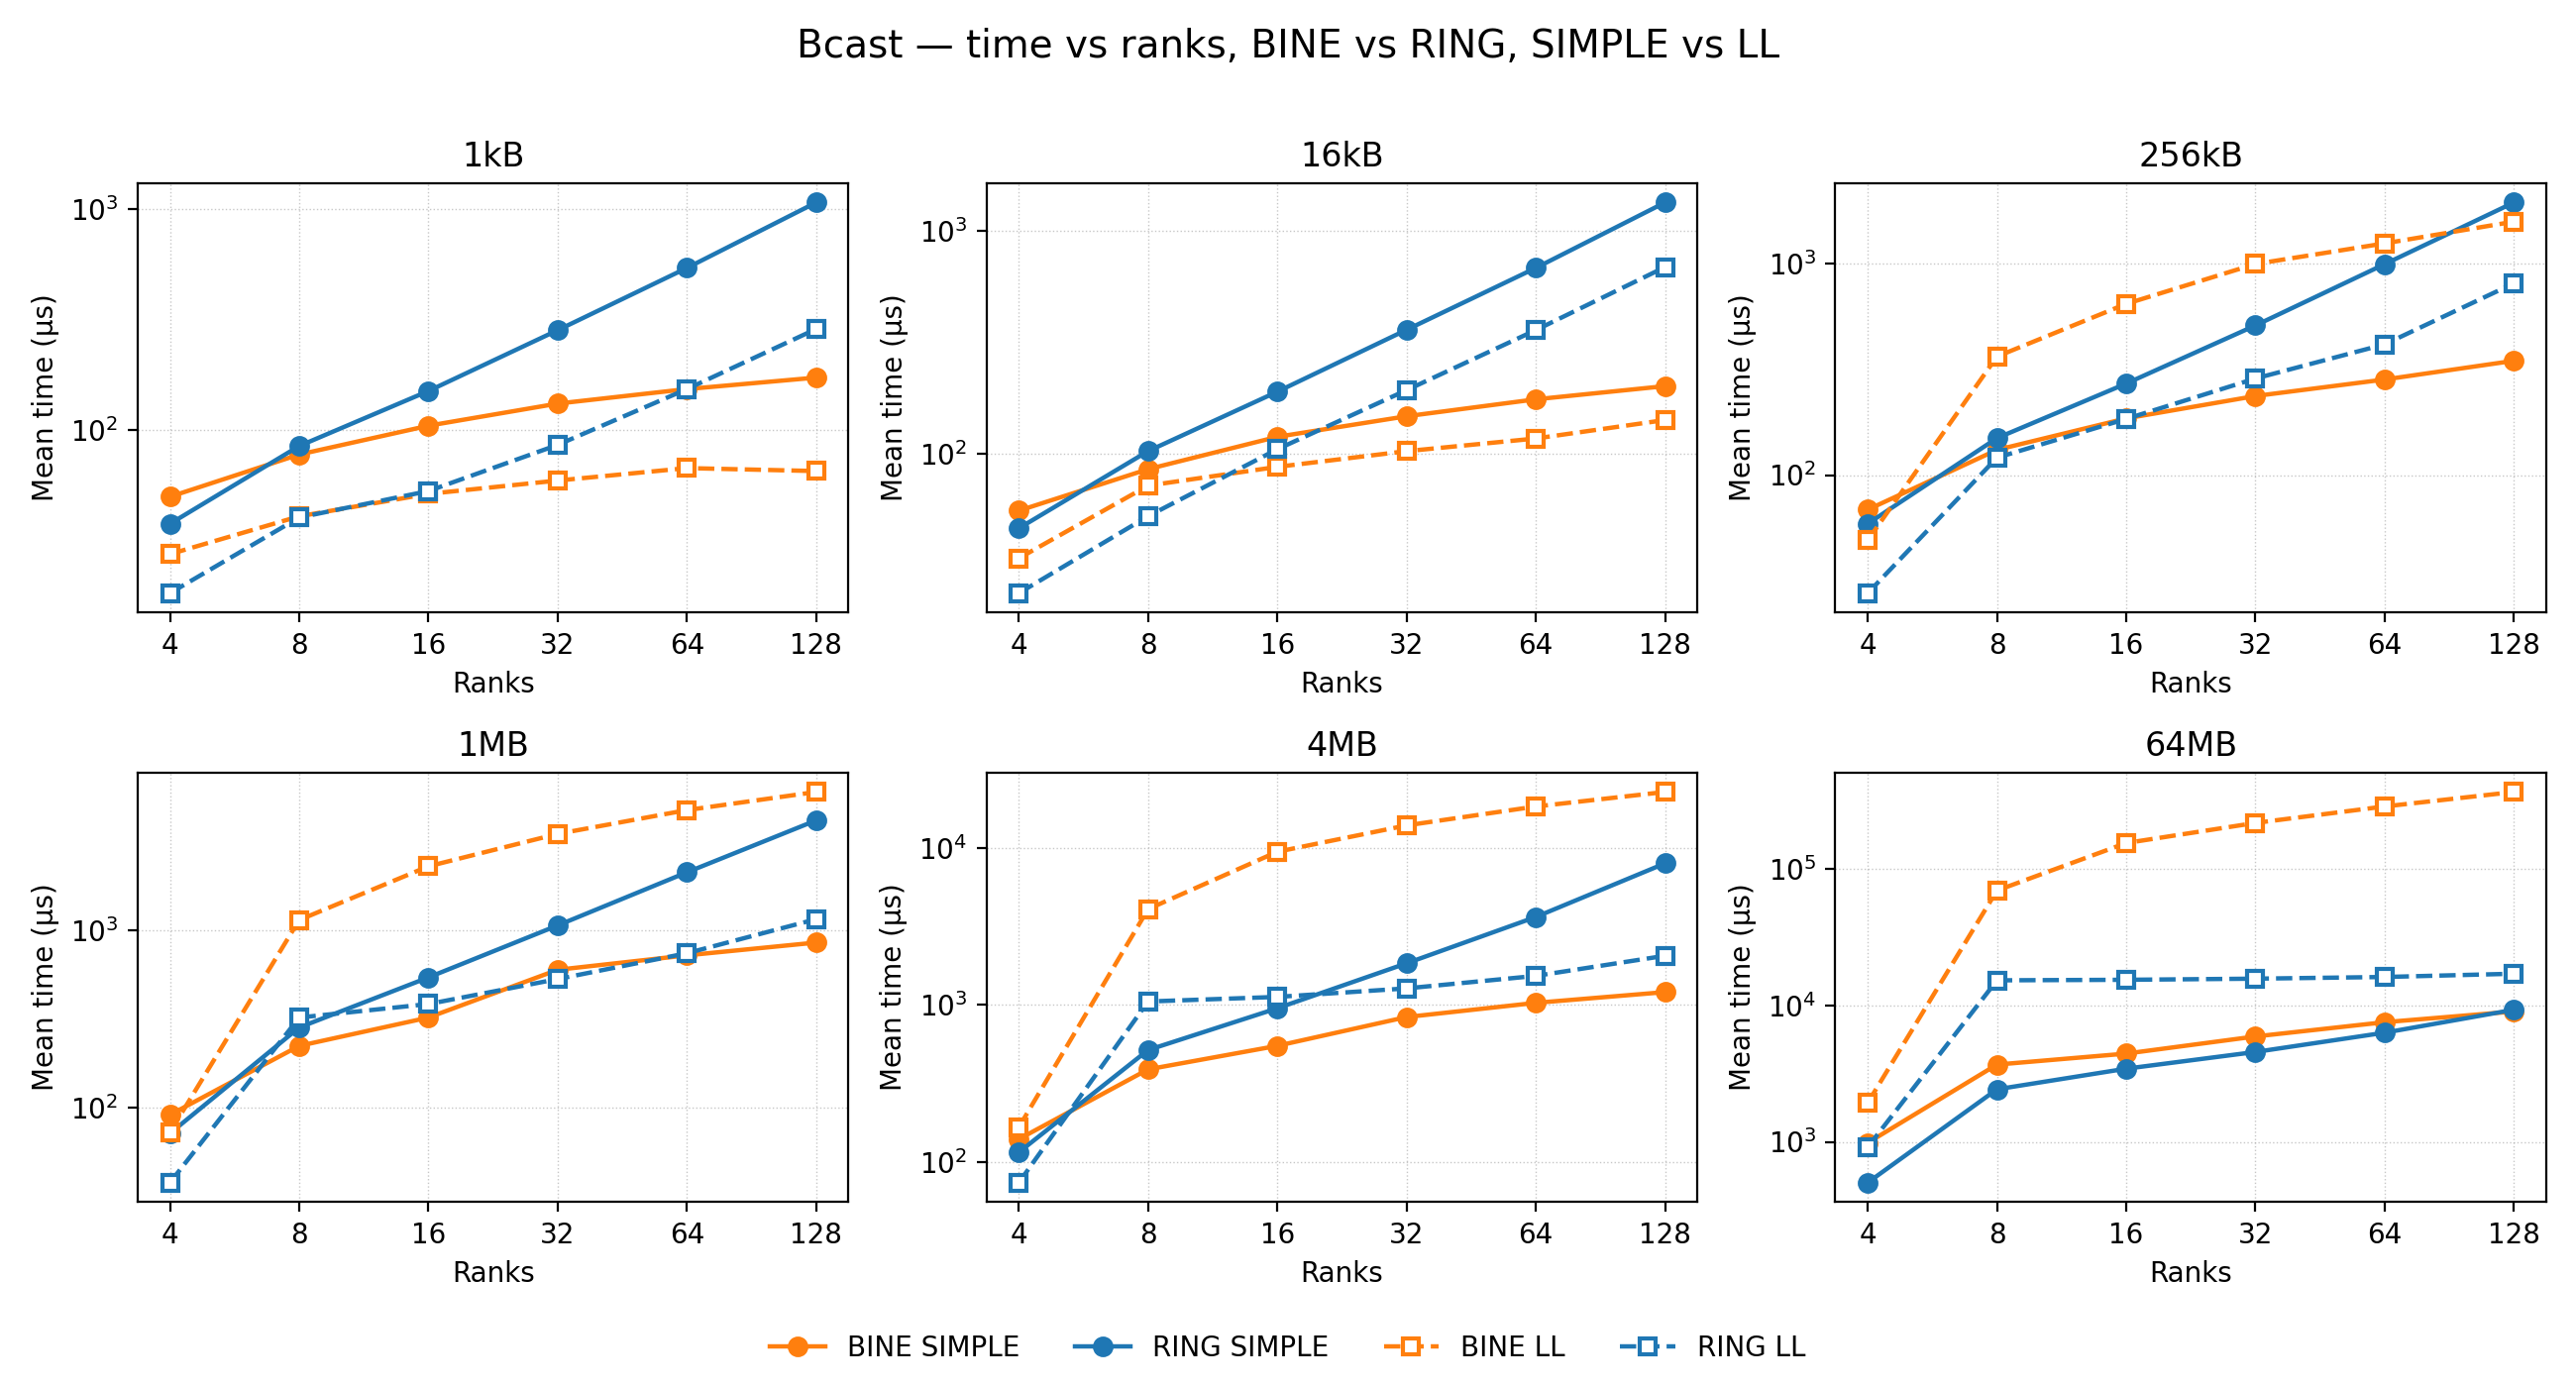
\includegraphics[width=\linewidth]{assets/plots/Bcast_SIMPLE_Ranks.png}
  \caption{Broadcast: median latency versus number of ranks, \bine{} (blue) against ring (red), for six message sizes. Solid lines with filled markers: \texttt{SIMPLE} protocol. Dashed lines with hollow markers: \texttt{LL} protocol.}
  \label{fig:tree-bcast}
\end{figure}

\begin{figure}[H]
  \centering
  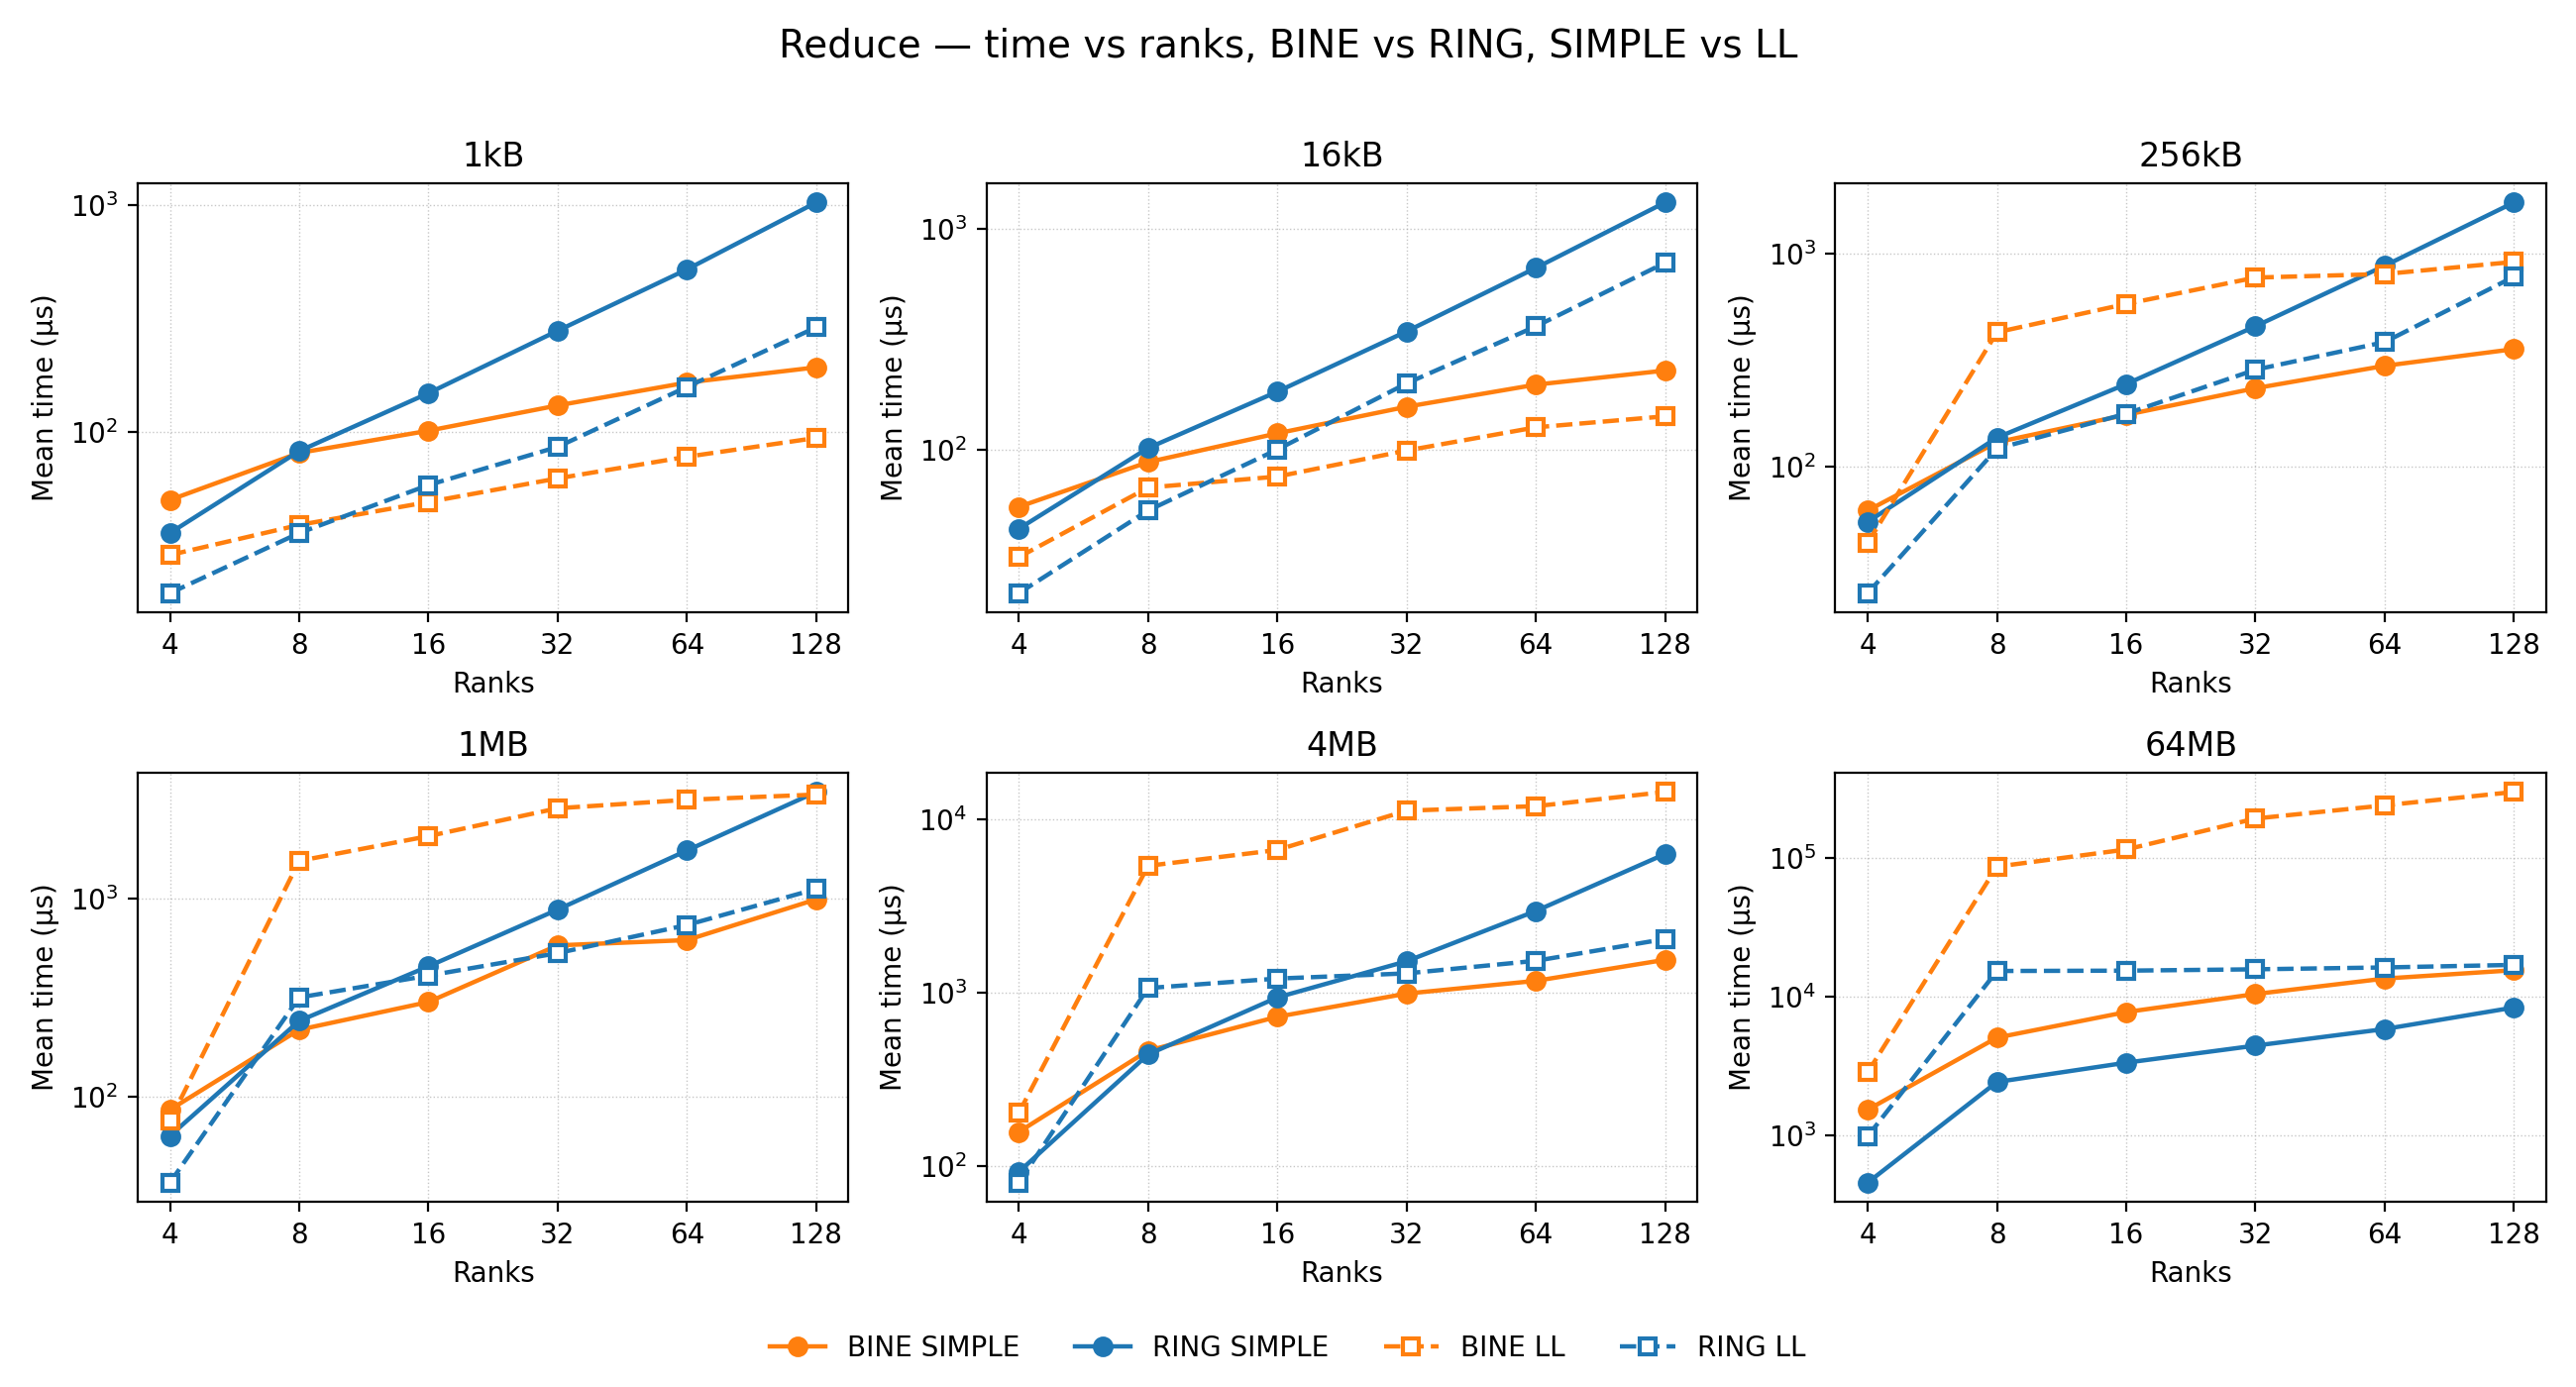
\includegraphics[width=\linewidth]{assets/plots/Reduce_SIMPLE_Ranks.png}
  \caption{Reduce: median latency versus number of ranks, \bine{} (blue) against ring (red), for six message sizes. Solid lines with filled markers: \texttt{SIMPLE} protocol. Dashed lines with hollow markers: \texttt{LL} protocol.}
  \label{fig:tree-reduce}
\end{figure}

\subsection{\texttt{SIMPLE} protocol}

The solid lines of \emph{Broadcast} ~\cref{fig:tree-bcast} and \emph{Reduce} ~\cref{fig:tree-reduce} show the expected separation between $\bigO{p}$ and $\bigO{\log p}$ (\cref{sec:bg-ring-vs-tree}).
Up to 4\,MB the ring time grows almost linearly with $p$ (about $2\times$ per doubling), while the \bine{} time grows by a roughly constant increment per doubling.
At $p=128$ \bine{} is faster by $5.9\times$, $6.5\times$, $5.5\times$, $4.8\times$ and $6\times$ at 1\,kB, 16\,kB, 256\,kB, 1\,MB and 4\,MB in the broadcast, and by $5.3\times$, $5.7\times$ and $4.9\times$ at 1\,kB, 16\,kB and 256\,kB, and by $3.4$--$3.5\times$ at 1\,MB and 4\,MB in the reduce.
At $p=4$ the ring is faster for all sizes, and the crossover lies between $4$ and $8$ ranks: with so few ranks the tree has few steps to save, and $p=4$ is also the only configuration that stays on NVLink.
The measurements do not separate the two effects.
At $p=8$ the two algorithms are within a few percent in the reduce up to 4\,MB.

At 64\,MB the operation is bandwidth-bound: every edge of the tree carries the whole buffer and the root forwards it $s$ times, whereas the pipelined ring moves each chunk once per link.
\bine{} is therefore slower than the ring in the broadcast for $p\le64$ ($2\times$ at $p=4$, $1.2$--$1.5\times$ for $p=8$ to $64$) and on par at $p=128$.
In the reduce it is slower at every scale ($1.8$--$3.4\times$), since the root also reduces $s$ full buffers in sequence while the ring spreads the reduction over all ranks.
Both algorithms jump sharply between $p=4$ and $p=8$, the cost of leaving NVLink for the network.

\subsection{\texttt{LL} protocol}\label{sec:tree-ll}

\texttt{LL} trades bandwidth for latency (\cref{sec:nccl-protocols}): half of the bytes it moves are flags.
The dashed lines of \cref{fig:tree-bcast,fig:tree-reduce} show that it helps both algorithms at small sizes, but degrades \bine{} much earlier and much more than the ring.

\paragraph{Small messages.}
Up to 16\,kB the picture is that of \texttt{SIMPLE} at lower absolute times.
At $p=128$ \bine{} is $4.4\times$ (broadcast) and $3.1\times$ (reduce) faster than the ring at 1\,kB and $4.9\times$ at 16\,kB, and \bine{} itself is $2.6\times$ and $1.4\times$ faster than with \texttt{SIMPLE} in the broadcast, at 1\,kB and 16\,kB respectively.
At small $p$ the ring is still better: at $p=4$ for all sizes, and at $p=8$ at 16\,kB (by $37\,\%$ in the broadcast and $27\,\%$ in the reduce).

\paragraph{Large messages.}
Above 16\,kB \bine{} scales worse than the ring.
At 64\,MB the ring is almost flat in $p$ (from 15.3 to 17.1\,ms in the broadcast between $p=8$ and $128$, about 4\,GB/s), while \bine{} grows from 69.6 to 367.7\,ms (from about 1.0 to 0.18\,GB/s), becoming $21.5\times$ slower in the broadcast and about $18\times$ in the reduce at $p=128$.
This is expected.
\texttt{LL} sustains a much lower bandwidth than \texttt{SIMPLE}, and the ring is the more bandwidth-efficient algorithm: each byte crosses each link once, while in the tree the root and the internal ranks send the buffer up to $s$ times, so the algorithm that moves more data pays more for the lower bandwidth.
For $p\ge8$ and 64\,MB the ring is slowed down by \texttt{LL} by $1.8$--$6.3\times$ with respect to \texttt{SIMPLE}, but \bine{} by $15$--$41\times$.
In addition, an intermediate rank of the ring uses the fused \texttt{directRecvCopyDirectSend} (\cref{sec:nccl-primitives}): it receives and forwards the same data in a single pass (under \texttt{LL}, which has no zero-copy path, this is the staged \texttt{recvCopySend}), so every rank receives and sends at the same time and a chunk streams through the ring. In \bine{}, instead, a rank either receives or sends at each step (fans $\langle1,0\rangle$ and $\langle0,1\rangle$, \cref{sec:tree-collectives}), with separate operations, so each hop of the tree is store-and-forward at the granularity of a chunk and no rank uses its receive and send directions simultaneously.
The slowdown follows the number of steps: at $p=4$ it is $2.1\times$ in the broadcast, about $s=2$, and it grows with $p$.

\paragraph{Crossover between \texttt{LL} and \texttt{SIMPLE}.}
As a consequence, \texttt{SIMPLE} overtakes \texttt{LL} much earlier for \bine{} than for the ring (\cref{tab:tree-ll-cross}): between 16 and 256\,kB for every $p\ge8$ for \bine{}, against between 256\,kB and 1\,MB at $p=8$ and between 4 and 64\,MB for $p\ge32$ for the ring.
The two collectives have the same crossover sizes.

\begin{table}[t]
\centering
\small
\caption{Largest measured message size for which \texttt{LL} is faster than \texttt{SIMPLE}. The crossover lies between this size and the next measured one (1\,kB, 16\,kB, 256\,kB, 1\,MB, 4\,MB, 64\,MB). The \bine{} and ring entries are the same for broadcast and reduce. The allgather (ring only, \cref{fig:tree-allgather}) was measured up to $p=32$, a dash means not measured.}
\label{tab:tree-ll-cross}
\begin{tabular}{@{}l cccccc@{}}
\toprule
 & $p=4$ & $8$ & $16$ & $32$ & $64$ & $128$ \\
\midrule
\bine{} (broadcast, reduce) & 1\,MB & 16\,kB  & 16\,kB & 16\,kB & 16\,kB & 16\,kB \\
Ring (broadcast, reduce) & 4\,MB & 256\,kB & 1\,MB  & 4\,MB  & 4\,MB  & 4\,MB  \\
Ring (allgather) & 1\,MB & 16\,kB & 16\,kB & 16\,kB & -- & -- \\
\bottomrule
\end{tabular}
\end{table}

\paragraph{Why the crossover differs: the ring allgather as a control.}\label{sec:tree-ll-allgather}
\cref{tab:tree-ll-cross} shows that the ring is not intrinsically tolerant of \texttt{LL}: the ring allgather (\cref{fig:tree-allgather}) switches to \texttt{SIMPLE} at the same sizes as \bine{}, at 16\,kB for every $p\ge8$ and at 1\,MB for $p=4$, and the ring with \texttt{LL} is slower than with \texttt{SIMPLE} from 256\,kB on at $p\ge8$ and from 4\,MB on at $p=4$.
Same protocols, same transport and same ring, but a different crossover from the ring broadcast and reduce.
The difference is therefore due to the algorithm, and the latency--bandwidth model of \cref{tab:bg-cost} explains it.
The size on the axis of \cref{fig:tree-allgather} is that of the block contributed by each rank, so $n=p\,m$ in the notation of \cref{tab:notation}.

\begin{figure}[H]
  \centering
  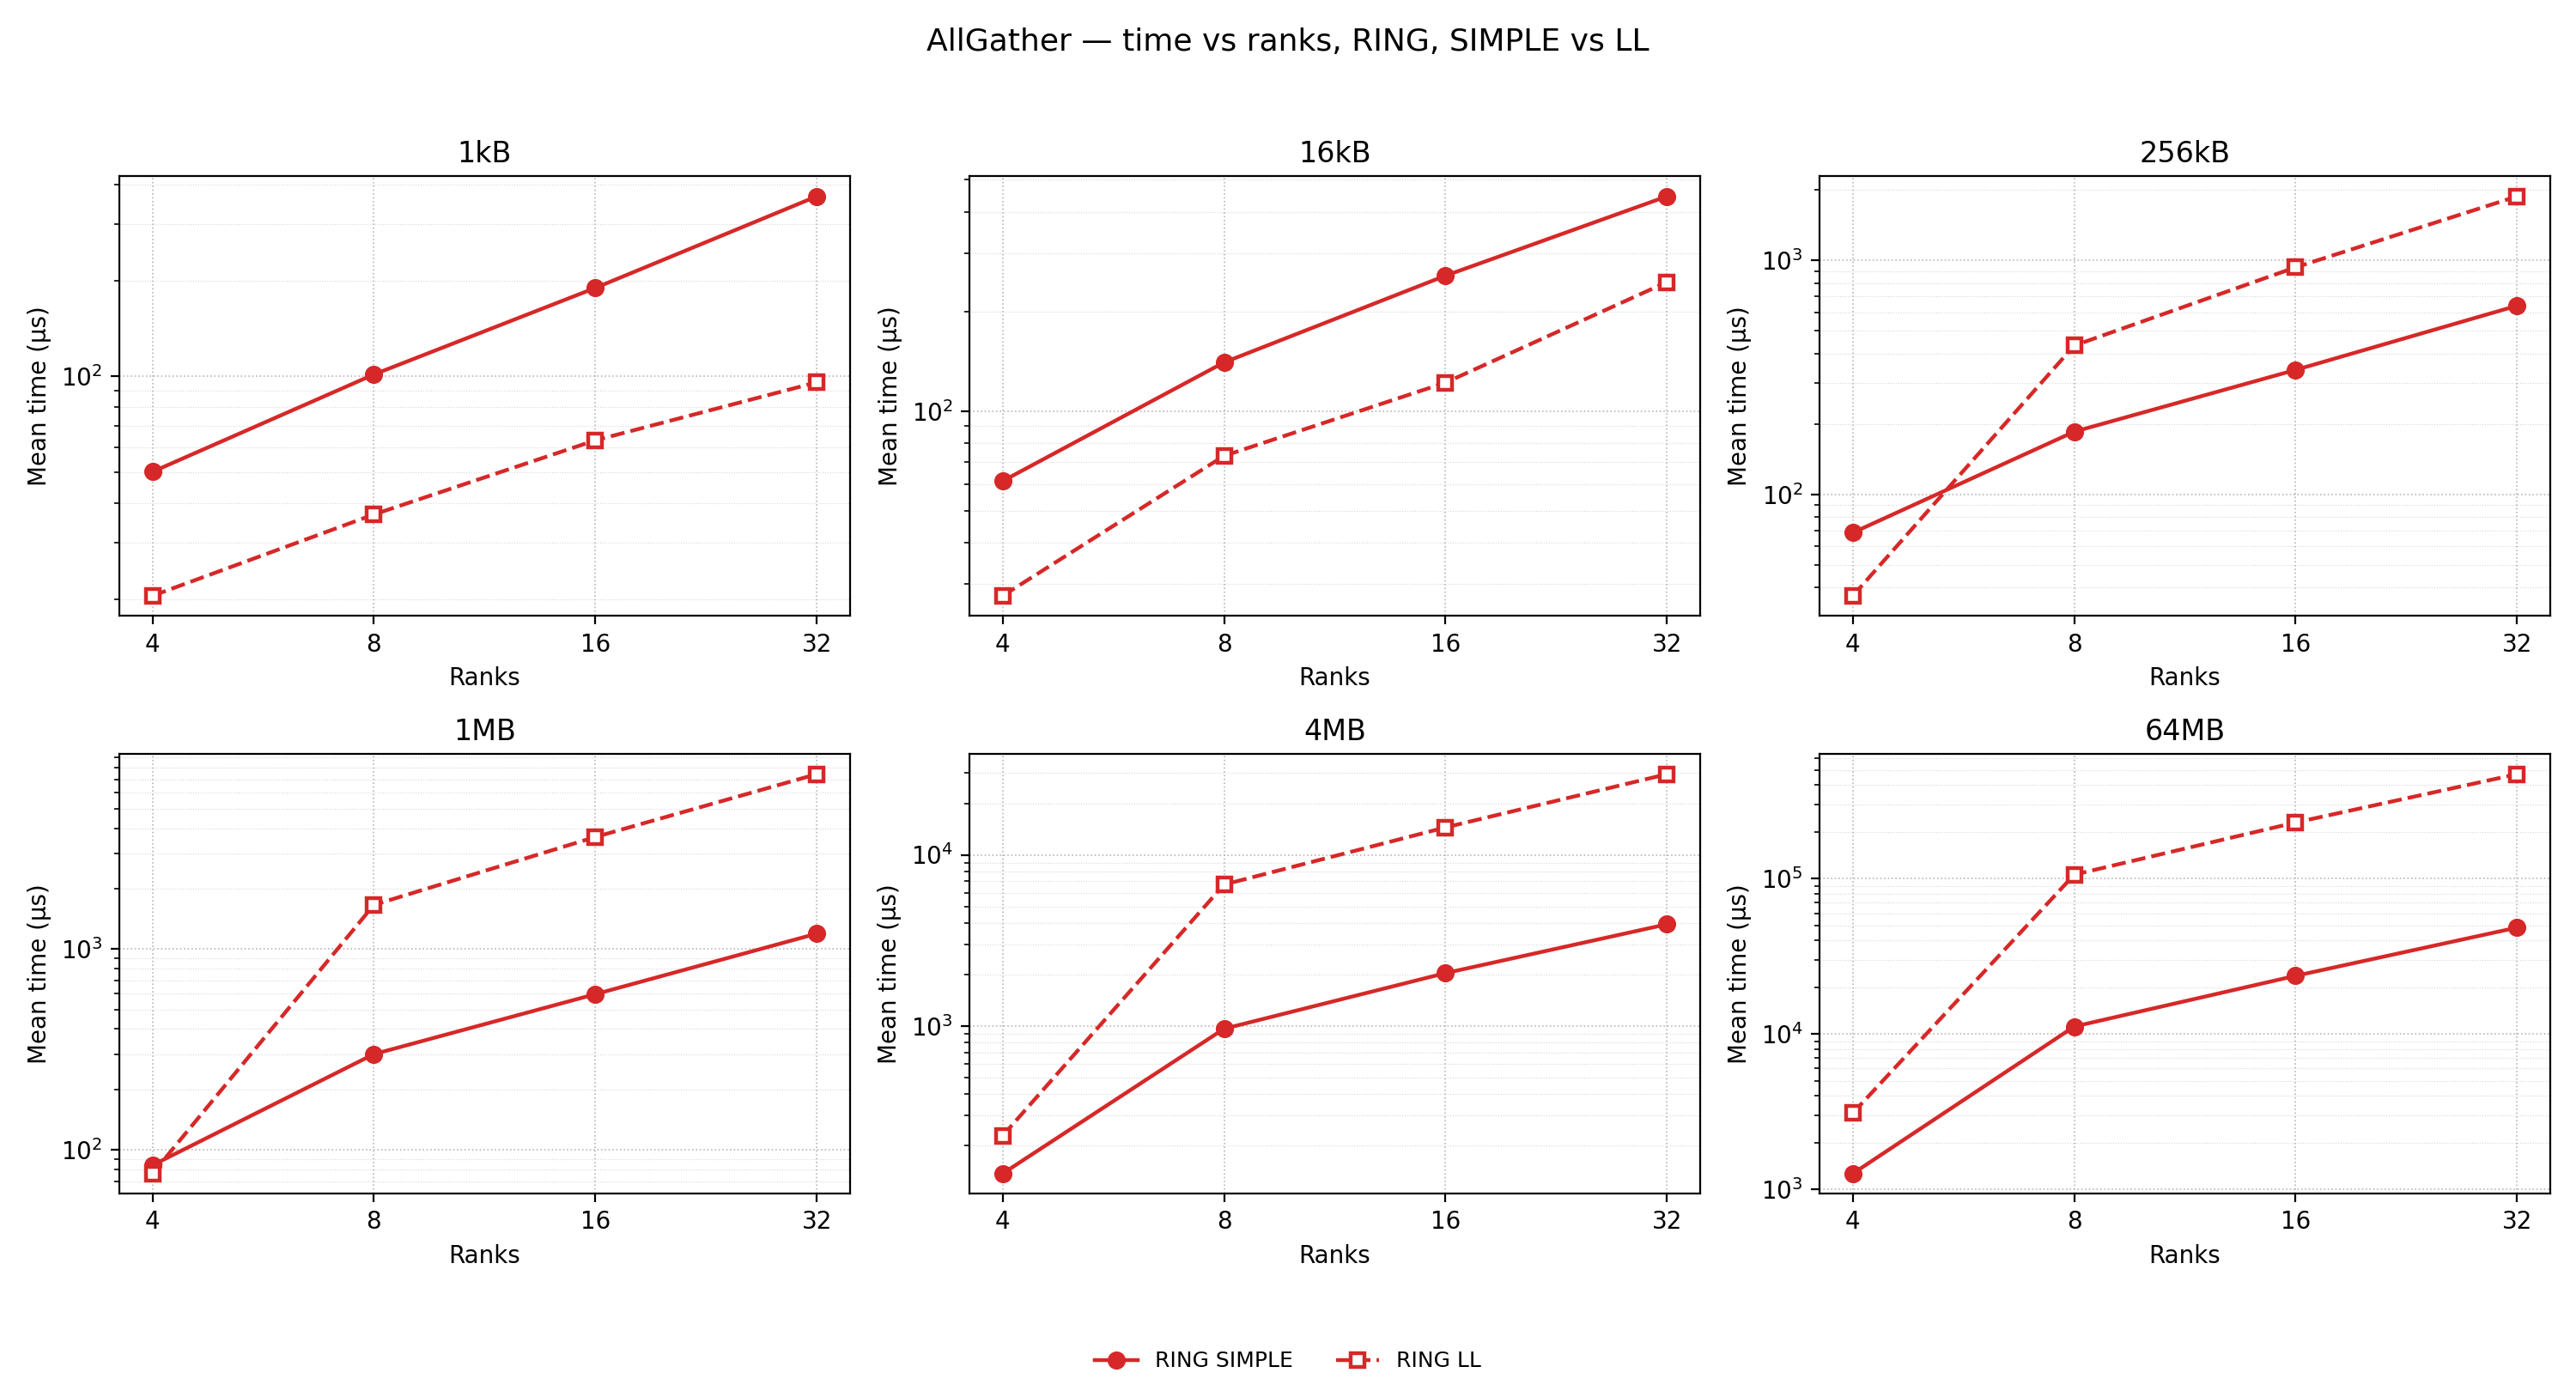
\includegraphics[width=\linewidth]{assets/plots/AllGather_SIMPLE_LL_Ranks.png}
  \caption{Ring allgather: median latency versus number of ranks, \texttt{SIMPLE} (solid, filled markers) against \texttt{LL} (dashed, hollow markers), for six block sizes, up to $p=32$.}
  \label{fig:tree-allgather}
\end{figure}

Let $(\alpha_S,\beta_S)$ and $(\alpha_L,\beta_L)$ be the latency and the time per byte of \texttt{SIMPLE} and \texttt{LL}, with $\alpha_L<\alpha_S$ and $\beta_L>\beta_S$.
The ring allgather and the tree broadcast have the same form: a number of steps, each paying $\alpha$ plus the transfer of a whole message,
\begin{equation}
  T_{\text{allgather}}=(p-1)\,(\alpha+m\beta),\qquad T_{\text{tree}}=s\,(\alpha+n\beta).
\end{equation}
For such an algorithm \texttt{LL} wins if $m<m^\ast=(\alpha_S-\alpha_L)/(\beta_L-\beta_S)$, and the number of steps cancels: both the latency saved and the bandwidth lost are paid at every step, so the crossover does not depend on $p$.
This is what we observe for the ring allgather and for \bine{}, whose crossover stays at 16\,kB from $p=8$ to $p=32$ (to the resolution of our size grid).
Expanding \cref{eq:bg-ring-bcast}, the pipelined ring broadcast has instead $T=(p+k-2)\,\alpha+n\beta+(p-2)\tfrac{n}{k}\beta$: the bandwidth cost of the vector is paid essentially once, because the chunks are amortised over the steps. Choosing $k$ near $k^\ast$ keeps the remaining terms small, so to first order the dependence on $p$ is the latency term $(p-2)\alpha$.
\texttt{LL} then saves about $(p-2)(\alpha_S-\alpha_L)$ and loses about $n(\beta_L-\beta_S)$, so the crossover $n^\ast$ grows with $p$, as in the ring row of \cref{tab:tree-ll-cross} (256\,kB at $p=8$, 4\,MB from $p=32$).
The same holds for the reduce, which adds $\tfrac{n}{k}\gamma$ per step and no new term in $p$.
To first order, then, the ring does not tolerate \texttt{LL} better than \bine{} because it is a ring, but because in the broadcast and in the reduce the chunks hide the bandwidth cost, while a collective in which every step moves a full block, like the allgather, does not.

\paragraph{The remaining gap: stepwise primitives.}
The allgather also gives the reference for the slowdown at 64\,MB, where the time is entirely bandwidth determined. Without amortisation, but with the fused primitive streaming through the ring, a ring with \texttt{LL} is about $9\times$ slower than with \texttt{SIMPLE} for $p\ge8$ (and about $2.5\times$ at $p=4$, which stays on NVLink).
\bine{} is slower than this, $15$--$41\times$ for $p\ge8$, and the excess grows with $p$.
This part is not explained by the model of \cref{tab:bg-cost} alone. It is an effect of how the tree kernel is built: at every step and for every chunk a new \texttt{Primitives} object is constructed with fans $\langle1,0\rangle$ (receive from the parent) or $\langle0,1\rangle$ (send to one child), so the tree is traversed as a sequence of separate point-to-point operations.
In the broadcast an internal rank first receives the chunk and then sends it to its children one step at a time. In the reduce it receives from its children one step at a time and sends the result up at the end.
Each hop is therefore store-and-forward, a rank never receives and sends at the same time (\cref{sec:tree-ll}, large messages), and the cost of setting up the primitive is paid at every step and chunk.
The ring, instead, builds one primitive per kernel and each byte streams through the fused \texttt{recvCopySend}, so the lower bandwidth of \texttt{LL} is paid once.
A fused tree kernel would build a single \texttt{Primitives} per rank with $\texttt{FanAsymmetric}\langle1,D\rangle$ in the broadcast ($\langle D,1\rangle$ in the reduce), where $D$ is the maximum number of children, receive once and forward to all children in one operation, so that a chunk streams through the tree and the setup is paid once. % TODO: add measurements of the fused kernel
In summary, the early crossover of \bine{} is the algorithmic cost of a collective without amortisation, shared with the ring allgather, and the additional slowdown at large sizes is due to the stepwise, store-and-forward structure of the kernel.

\paragraph{Effect on the speedup.}
If each algorithm uses its best protocol (\cref{tab:tree-best}), \bine{} remains faster than the ring at $p=128$ for all sizes except the 64\,MB reduce, where the ring is $1.8\times$ faster, in the 64\,MB broadcast the two are on par.
The margin at medium sizes is smaller than with \texttt{SIMPLE} alone, since the ring can use \texttt{LL} up to 4\,MB while \bine{} cannot, but it remains significant: at 1--4\,MB the speedup goes from $4.6$--$6.5\times$ to $1.3$--$1.6\times$, and it reaches $5\times$ at 16\,kB.
At $p=8$ the ring with \texttt{LL} is ahead of \bine{} up to 256\,kB, by at most $1.18\times$ in the broadcast and $1.09\times$ in the reduce, while \bine{} is faster at 1\,MB and, in the broadcast, at 4\,MB.
At 64\,MB the best protocol is \texttt{SIMPLE} for both algorithms, so the choice of protocol does not change the comparison.

\begin{table}[t]
\centering
\small
\caption{Best protocol of each algorithm and speedup of \bine{} over the ring, both with their best protocol, at $p=128$. A value below $1$ means that the ring is faster.}
\label{tab:tree-best}
\begin{tabular}{@{}r ccc @{\qquad} ccc@{}}
\toprule
 & \multicolumn{3}{c}{Broadcast} & \multicolumn{3}{c}{Reduce} \\
\cmidrule(lr){2-4}\cmidrule(l){5-7}
Size & \bine{} & Ring & Speedup & \bine{} & Ring & Speedup \\
\midrule
1\,kB   & \texttt{LL}     & \texttt{LL}     & $4.4\times$ & \texttt{LL}     & \texttt{LL}     & $3.1\times$ \\
16\,kB  & \texttt{LL}     & \texttt{LL}     & $4.9\times$ & \texttt{LL}     & \texttt{LL}     & $4.9\times$ \\
256\,kB & \texttt{SIMPLE} & \texttt{LL}     & $2.3\times$ & \texttt{SIMPLE} & \texttt{LL}     & $2.2\times$ \\
1\,MB   & \texttt{SIMPLE} & \texttt{LL}     & $1.4\times$ & \texttt{SIMPLE} & \texttt{LL}     & $1.1\times$ \\
4\,MB   & \texttt{SIMPLE} & \texttt{LL}     & $1.7\times$ & \texttt{SIMPLE} & \texttt{LL}     & $1.3\times$ \\
64\,MB  & \texttt{SIMPLE} & \texttt{SIMPLE} & $1.0\times$ & \texttt{SIMPLE} & \texttt{SIMPLE} & $0.54\times$ \\
\bottomrule
\end{tabular}
\end{table}

\subsection{Summary}

With \texttt{SIMPLE}, \bine{} is the better choice for small and medium messages (up to a few MB) from $8$ ranks on, with speedups of $3.4$--$6.5\times$ at $128$ ranks and logarithmic scaling, while for 64\,MB the ring is better or equal, the reduce being the worse case. At $p=4$ the ring always wins, but this configuration is entirely intra-node and not representative.
\texttt{LL} helps \bine{} only up to 16\,kB, where it is up to $4.9\times$ faster than the ring at $128$ ranks.
Above that the ring, being more bandwidth-efficient, keeps benefiting from \texttt{LL} up to 4\,MB while \bine{} must switch to \texttt{SIMPLE} (the ring allgather, which has no chunk amortisation, switches as early as \bine{}, so the early crossover is algorithmic, and the extra slowdown of \bine{} at large sizes is the fan-out and fan-in of the tree), so with each algorithm at its best protocol the advantage at 1--4\,MB falls to $1.1$--$1.7\times$, and at $p=8$ it vanishes below 1\,MB.
This motivates the bandwidth-optimal butterfly-style algorithms of \cref{ch:butterfly}, and a selection rule based on message size, number of ranks and protocol, not on the algorithm alone.

\chapter{Bine Butterfly Algorithms}\label{ch:butterfly}

% From this chapter on, float-only pages stack their floats from the top
% instead of spreading them over the page.
\makeatletter
\setlength{\@fptop}{0pt}
\setlength{\@fpsep}{20pt plus 2pt}
\setlength{\@fpbot}{0pt plus 1fil}
\makeatother

% Channel colours used by the figures of this chapter
\colorlet{pch0}{ch0!70}
\colorlet{pch1}{ch1!70}
\colorlet{pch2}{ch2!70}
\colorlet{pch3}{chunkB!90}

This chapter implements the \bine{} butterfly of \cref{sec:bg-bine-butterfly} in \nccl{} for the allgather, the reduce-scatter and the allreduce.
\Cref{sec:bfly-impl} describes the schedule of the distance-doubling butterfly, \cref{sec:bfly-collectives} how it is turned into kernels, \cref{sec:bfly-dhlv} the distance-halving schedule used by the double send strategy, and \cref{sec:bfly-testing} the invariants that the schedule satisfies.

%==============================================================================
\section{Schedule construction}\label{sec:bfly-impl}

As for the tree, the schedule is built for $p=2^s$ ranks and is defined only for powers of two.
Unlike the tree, a butterfly has no root, so there is no rotation: one set of tables serves every collective on the communicator.

\subsection{Output and notation}

The schedule consists of a table and two vectors,
\begin{align}
  \Pi(r,i) &\in \{0,\dots,p-1\}, \\
  \nu(r) &\in \{0,\dots,p-1\}, \qquad \nu^{-1}(x)\in\{0,\dots,p-1\},
\end{align}
for $r\in[0,p-1]$ and $i\in[0,s-1]$.
$\Pi(r,i)=q$ means that rank $r$ exchanges data with rank $q$ at step $i$, and $\nu$ is a rank-dependent label (\cref{sec:bfly-def}) with inverse $\nu^{-1}$.
All the ranks communicate at all the steps, so the table has no empty entries, unlike the tables of the tree (\cref{sec:tree-impl}).
The arrays are filled by
\begin{verbatim}
void ncclGetBineButterflyDdbl(int nRanks, int steps,
                              int *partners, int *index, int *order);
\end{verbatim}
which writes \texttt{partners} (the table $\Pi$), \texttt{index} (the vector $\nu$) and \texttt{order} (the vector $\nu^{-1}$).
Step $i$ is the $i$-th step of the reduce-scatter, where the distance between partners grows. The allgather is its reverse.

\subsection{Definition}\label{sec:bfly-def}

Let
\begin{equation}
  \rho_i=\sum_{k=0}^{i}(-2)^k=\frac{1-(-2)^{i+1}}{3}.
  \label{eq:bfly-rho}
\end{equation}
The partner of rank $r$ at step $i$ is
\begin{equation}
  \Pi(r,i)=
  \begin{cases}
    (r+\rho_i)\bmod p & \text{if $r$ is even},\\
    (r-\rho_i)\bmod p & \text{if $r$ is odd}.
  \end{cases}
  \label{eq:bfly-partner}
\end{equation}
This is the partner of \cref{eq:bg-bine-bfly-partner} with the steps in the opposite order, since $\rho_i=\tau_{s-1-i}$ (\cref{eq:bg-bine-tau}), that is, $\Pi(r,i)=\pi_{s-1-i}(r)$.
The distance $\lvert\rho_i\rvert\approx 2^{i+1}/3$ grows with $i$.

The label $\nu$ is the position of a rank in the distance-doubling \bine{} tree rooted at rank $0$~\cite{desensi2025bine}.
With
\begin{equation}
  h(r)=
  \begin{cases}
    0 & \text{if } r=0,\\
    \rtn(p-r) & \text{if $r$ is even and } r\neq0,\\
    \rtn(r) & \text{if $r$ is odd,}
  \end{cases}
  \qquad
  \nu(r)=h(r)\oplus\bigl(h(r)\gg1\bigr),
  \label{eq:bfly-nu}
\end{equation}
where $\gg$ is the logical right shift, and $\nu^{-1}$ is its inverse (it exists by invariant~\ref{inv:bfly-perm}).
The labels define where the block of a rank is stored in the kernels: the \emph{position} of the block of rank $r$ is
\begin{equation}
  \mathrm{pos}(r)=\mathrm{rev}(\nu(r)),
\end{equation}
where $\mathrm{rev}$ reverses the $s$ bits.
We will see that the blocks exchanged at a step are contiguous in the position space and, in general, not in the rank space.

\subsection{Example: \texorpdfstring{$p=8$}{p = 8}}

For $p=8$ ($s=3$), $\rho_0=1$, $\rho_1=-1$ and $\rho_2=3$.
\Cref{tab:bfly-nu-p8} gives the labels and the positions, and \cref{fig:bfly-butterfly} the partners.
For example, rank $3$ is odd and communicates with $3-1=2$, $3+1=4$ and $3-3=0$.

\begin{table}[t]
\centering
\small
\caption{Values $h(r)$ and $\nu(r)$ (binary) and position $\mathrm{pos}(r)=\mathrm{rev}(\nu(r))$ (decimal) for $p=8$. The inverse is $\nu^{-1}=[0,1,7,2,3,6,4,5]$.}
\label{tab:bfly-nu-p8}
\begin{tabular}{@{}l*{8}{c}@{}}
\toprule
$r$ & 0 & 1 & 2 & 3 & 4 & 5 & 6 & 7 \\
\midrule
$h(r)$ & 000 & 001 & 010 & 111 & 100 & 101 & 110 & 011 \\
$\nu(r)$ & 000 & 001 & 011 & 100 & 110 & 111 & 101 & 010 \\
$\mathrm{pos}(r)$ & 0 & 4 & 6 & 1 & 3 & 7 & 5 & 2 \\
\bottomrule
\end{tabular}
\end{table}

\begin{figure}[t]
\centering
\begin{tikzpicture}[x=2.3cm, y=-0.62cm, font=\footnotesize,
    rk/.style={circle, draw, fill=white, minimum size=0.6cm, inner sep=0pt}]
  % partner edges: column i -> column i+1
  \foreach \r/\q in {0/1,1/0,2/3,3/2,4/5,5/4,6/7,7/6}
    \draw[ch0, thick] (0,\r) -- (1,\q);
  \foreach \r/\q in {0/7,1/2,2/1,3/4,4/3,5/6,6/5,7/0}
    \draw[ch1, thick] (1,\r) -- (2,\q);
  \foreach \r/\q in {0/3,1/6,2/5,3/0,4/7,5/2,6/1,7/4}
    \draw[ch2, thick] (2,\r) -- (3,\q);
  % nodes
  \foreach \c in {0,...,3}
    \foreach \r in {0,...,7}
      \node[rk] at (\c,\r) {\r};
  % labels
  \node[ch0] at (0.5,-1.1) {$i=0$, $\lvert\rho_0\rvert=1$};
  \node[ch1] at (1.5,-1.1) {$i=1$, $\lvert\rho_1\rvert=1$};
  \node[ch2] at (2.5,-1.1) {$i=2$, $\lvert\rho_2\rvert=3$};
\end{tikzpicture}
\caption{Distance-doubling \bine{} butterfly for $p=8$. An edge from rank $r$ in column $i$ to rank $q$ in column $i+1$ means $\Pi(r,i)=q$. The reduce-scatter reads the figure from left to right, the allgather from right to left.}
\label{fig:bfly-butterfly}
\end{figure}

\subsection{Computing the tables}

\Cref{alg:bfly-schedule} computes the three arrays.
The labels are computed first and $\nu^{-1}$ is obtained by inverting them. Then the partners are computed one step at a time, accumulating $\rho_i$ in a 64-bit integer and reducing it modulo $p$ with a non-negative result.
The cost is $O(p\log p)$ time and memory.

\begin{algorithm}[t]
\caption{Schedule of the distance-doubling \bine{} butterfly ($p=2^s$).}
\label{alg:bfly-schedule}
\begin{algorithmic}[1]
\Require $p=2^s$
\Ensure table $\Pi$ of size $p\times s$, vectors $\nu$ and $\nu^{-1}$ of size $p$
\For{$r\gets 0$ \textbf{to} $p-1$}
  \State compute $h(r)$ \Comment{\cref{eq:bfly-nu}}
  \State $\nu(r)\gets h(r)\oplus(h(r)\gg1)$;\quad $\nu^{-1}(\nu(r))\gets r$
\EndFor
\State $\rho\gets0$;\quad $w\gets1$
\For{$i\gets 0$ \textbf{to} $s-1$}
  \State $\rho\gets\rho+w$;\quad $w\gets-2w$ \Comment{$\rho=\rho_i$}
  \State $m\gets\rho\bmod p$ \Comment{non-negative}
  \For{$r\gets 0$ \textbf{to} $p-1$}
    \State $\Pi(r,i)\gets (r+m)\bmod p$ \textbf{if} $r$ is even, \textbf{else} $(r-m)\bmod p$
  \EndFor
\EndFor
\end{algorithmic}
\end{algorithm}

%==============================================================================
\section{Allgather, reduce-scatter and allreduce}\label{sec:bfly-collectives}

The table says who communicates with whom. Which data moves is decided by the collective.
\begin{itemize}
  \item \emph{Allgather.} Each rank contributes a block of \texttt{count} elements and obtains the $p$ blocks, the block of rank $b$ at offset $b\cdot\texttt{count}$ of \texttt{recvbuff}.
  \item \emph{Reduce-scatter.} Each rank holds $p$ blocks, and rank $b$ obtains the reduction of the blocks $b$ of all the ranks.
  \item \emph{Allreduce.} Each rank obtains the elementwise reduction of the vectors of all the ranks. It is a reduce-scatter followed by an allgather (\cref{sec:bfly-allreduce}).
\end{itemize}

\subsection{Integration in NCCL}

The butterfly is integrated as the tree (\cref{sec:tree-integration}), with the same algorithm \texttt{NCCL\_ALGO\_BINE} and pattern \texttt{ncclPatternBine}, and three pieces.
\begin{itemize}
  \item \emph{Pattern.} \texttt{ncclPatternBine}, used by the host to compute the number of steps and the chunking.
  \item \emph{Tables.} The tables of \cref{sec:bfly-impl,sec:bfly-dhlv} are stored in \texttt{channel.bine} next to those of the tree: \texttt{partners} ($\Pi$), \texttt{dhlvPartners} ($\Pi^{\mathrm{dh}}$), \texttt{index} ($\nu$) and \texttt{order} ($\nu^{-1}$).
  The fields \texttt{nSteps} and \texttt{nDoublingSteps} are both set to $s$, and the kernels use the latter.
  \item \emph{\texttt{RunWorkColl} specialisations.} One for each collective and protocol, as for the tree, which call the kernel of the strategy of \cref{sec:bfly-strategies} (send, permute, block-by-block or double send).
\end{itemize}

\subsection{Blocks, positions and strategies}\label{sec:bfly-strategies}

\paragraph{Allgather as the reverse of the reduce-scatter.}
Step $k\in[0,s-1]$ of the allgather uses the partner $\Pi(r,s-1-k)$: the distance decreases and the data doubles at each step.
At step $k$ a rank holds $g=2^k$ blocks, sends them and receives the $g$ blocks of its partner.
The reduce-scatter is the time reverse: step $i$ uses $\Pi(r,i)$, and the data halves.

\paragraph{Contiguity in the position space.}
Let $x=\mathrm{pos}(r)$ and $y=\mathrm{pos}(q)$ for $q=\Pi(r,s-1-k)$.
Bit $b$ of $\nu$ is bit $s-1-b$ of $\mathrm{pos}$, so invariant~\ref{inv:bfly-split} with $i=s-1-k$ says that $x$ and $y$ agree above bit $k$ and differ at bit $k$.
Hence the $g$ blocks held at step $k$ are those whose positions lie in the aligned range of size $g$ containing $x$, and the blocks of the partner lie in the sibling range (\cref{fig:bfly-held}).
In the position space the pattern is a recursive-doubling allgather. In the rank space, the blocks of an aligned range are the ranks $\nu^{-1}(\mathrm{rev}(y))$, which are in general not contiguous.

\begin{figure}[t]
\centering
\begin{tikzpicture}[x=1.05cm, y=0.95cm, font=\footnotesize,
    cell/.style={draw, minimum width=1cm, minimum height=0.8cm, inner sep=0pt, align=center}]
  \foreach \row/\n in {0/1,1/2,2/4,3/8}
    \foreach \y/\b in {0/0,1/3,2/7,3/4,4/1,5/6,6/2,7/5} {
      \ifnum\y<\n \def\fc{ch0!35}\else\def\fc{white}\fi
      \node[cell, fill=\fc] at (\y,-\row) {$\y$\\[-1pt]{\tiny $r{=}\b$}};
    }
  \node[anchor=east] at (-0.7,0)  {start};
  \node[anchor=east] at (-0.7,-1) {after $k{=}0$};
  \node[anchor=east] at (-0.7,-2) {after $k{=}1$};
  \node[anchor=east] at (-0.7,-3) {after $k{=}2$};
  \node[anchor=west] at (7.7,-1) {$q=3$ (pos.\ 1)};
  \node[anchor=west] at (7.7,-2) {$q=7$ (pos.\ 2)};
  \node[anchor=west] at (7.7,-3) {$q=1$ (pos.\ 4)};
\end{tikzpicture}
\caption{Blocks held by rank $0$ (position $0$) during the allgather with $p=8$. Cell $y$ is a position. $r$ is the rank whose block it contains, $\nu^{-1}(\mathrm{rev}(y))$. The held positions (shaded) always form an aligned range, whereas the held ranks $\{0\}$, $\{0,3\}$, $\{0,3,7,4\}$ are not contiguous. The right column is the partner at each step.}
\label{fig:bfly-held}
\end{figure}

\paragraph{Strategies.}
The strategies differ in where they put the blocks, not in the pattern.
Each is defined by the \emph{slot} of position $y$ (the block-sized region of the working buffer used for it), a \emph{pre-step} that puts the data in the right slots, and a \emph{post-step} that restores the natural order (\cref{tab:bfly-strategies}).
\begin{itemize}
  \item \emph{Send} exchanges the blocks before the butterfly: $r$ sends its block to $\nu^{-1}(\mathrm{rev}(r))$ and receives that of rank $\mathrm{pos}(r)$, stored at slot $\mathrm{pos}(r)$.
  Ranks with $\mathrm{pos}(r)=r$ need no exchange.
  \item \emph{Permute} stores the block at slot $\mathrm{pos}(r)$ and permutes the blocks in place at the end.
  \item \emph{Block-by-block} keeps the natural order, so the slot of position $y$ is $\nu^{-1}(\mathrm{rev}(y))$ and every block is sent separately.
  \item \emph{Double send} keeps the natural order with the distance-halving schedule, whose windows are contiguous modulo $p$ (\cref{sec:bfly-dhlv}).
\end{itemize}
In the reduce-scatter the roles of exchange and permutation are mirrored: the exchange of \emph{send} becomes a post-step, and the permutation of \emph{permute} a pre-step.
When a reduce-scatter is followed by an allgather, as in the allreduce, the exchange of \emph{send} cancels out~\cite{desensi2025bine}.

\paragraph{Fused copies.}
The copy of the own block is not a separate pass in the allgather: it is fused into the first send (\texttt{copySend}), which reads \texttt{sendbuff}, writes the slot and sends.
It is executed separately, followed by a barrier, only when it cannot be fused: in place, where a direct write of the partner could overwrite the source.
In the reduce-scatter the last receive writes the reduced block directly in \texttt{recvbuff} (except in \emph{send}, which is followed by the exchange).

\begin{table}[t]
\centering
\footnotesize
\setlength{\tabcolsep}{4pt}
\caption{The strategies as choices of slot, pre-step and post-step. Send, permute and block-by-block use the distance-doubling table (reversed in the allgather). Double send uses the distance-halving one. Copies are fused as described in the text.}
\label{tab:bfly-strategies}
\begin{tabularx}{\linewidth}{@{}l l X X l@{}}
\toprule
Strategy & Slot of $y$ & Allgather & Reduce-scatter & Unit \\
\midrule
Send & $y$ & pre: exchange with $\nu^{-1}(\mathrm{rev}(r))$ & post: same exchange & run \\
Permute & $y$ & pre: copy to slot $\mathrm{pos}(r)$, post: permutation & pre: permutation, post: copy slot $\mathrm{pos}(r)$ & run \\
Block-by-block & $\nu^{-1}(\mathrm{rev}(y))$ & pre: copy to slot $r$ & post: copy slot $r$ & block \\
Double send & circular window & pre: copy to slot $r$ & post: copy slot $r$ & $\le2$ runs \\
\bottomrule
\end{tabularx}
\end{table}

\subsection{Work partition}\label{sec:bfly-pos}

By default a channel handles a slice of \emph{every} block (\emph{slice mode}).
A range of $g$ positions is then $g$ pieces separated by a stride of \texttt{count}, contiguous only if \texttt{channelCount}$=$\texttt{count}.
For small messages this multiplies the number of calls by the number of channels.

Send, double send and block-by-block therefore have a second partition, \emph{pos mode}, in which a channel handles \emph{whole} blocks of a range of positions (\cref{fig:bfly-partition}): with $n_c$ channels, channel $j$ owns the positions $[j\lceil p/n_c\rceil,(j+1)\lceil p/n_c\rceil)$, clipped to $p$.
The part of a window owned by a channel is then one contiguous run for the strategies whose slots are the positions.
Pos mode is selected when
\begin{equation}
  n_c>1,\qquad p\ge n_c,\qquad \texttt{count}\cdot\texttt{sizeof}(T)<n_c\cdot S,
  \label{eq:bfly-pos}
\end{equation}
where $S$ is a threshold (\texttt{BINE\_POS\_SLICE\_BYTES}).
In other words, a block is partitioned by position only when its slice per channel, $\texttt{count}\cdot\texttt{sizeof}(T)/n_c$, would be smaller than $S$, and the block size at which the partition changes is $n_c S$.
The condition depends only on values equal on all ranks and channels.

The value of $S$ was determined experimentally: we swept it and measured, for each value, the latency of the strategies in both partitions.
The two partitions cross at about $S=16\,\text{KiB}$ per channel, which is the default value.
$S$ is a compile-time parameter: \texttt{BINE\_POS\_SLICE\_BYTES} is defined with this default only if it is not already defined, so it can be changed at build time (e.g., with \texttt{-DBINE\_POS\_SLICE\_BYTES=}$\langle\text{bytes}\rangle$) without touching the source, and the crossover can differ on other systems.
Below it pos mode wins, since a contiguous run needs fewer calls than the strided pieces of slice mode (\cref{sec:bfly-res-modes}). Above it the idle channels of pos mode cost more than the calls it saves, so slice mode wins.

\begin{figure}[t]
\centering
\begin{tikzpicture}[x=0.95cm, y=0.9cm, font=\footnotesize]
  % legend
  \foreach \c in {0,...,3} {
    \fill[pch\c] (2.2*\c,1.9) rectangle ++(0.3,0.3);
    \node[anchor=west] at (2.2*\c+0.3,2.05) {channel \c};
  }
  % (a) slice mode
  \node[anchor=south west] at (0,0.75) {(a) slice mode};
  \foreach \y in {0,...,7} {
    \foreach \c in {0,...,3}
      \fill[pch\c] (\y+0.25*\c,0) rectangle ++(0.25,0.6);
    \draw (\y,0) rectangle ++(1,0.6);
    \node[below] at (\y+0.5,0) {\y};
  }
  \draw[decorate, decoration={brace, amplitude=4pt}] (8,-0.65) -- (4,-0.65)
    node[midway, below=4pt, align=center] {window of 4 positions:\\every channel moves 4 strided pieces};
  % (b) pos mode
  \begin{scope}[yshift=-4.3cm]
    \node[anchor=south west] at (0,0.75) {(b) pos mode};
    \foreach \y/\c in {0/0,1/0,2/1,3/1,4/2,5/2,6/3,7/3} {
      \fill[pch\c] (\y,0) rectangle ++(1,0.6);
      \draw (\y,0) rectangle ++(1,0.6);
      \node[below] at (\y+0.5,0) {\y};
    }
    \draw[decorate, decoration={brace, amplitude=4pt}] (8,-0.65) -- (4,-0.65)
      node[midway, below=4pt, align=center] {window of 4 positions:\\channels 2 and 3 move one contiguous run each};
  \end{scope}
\end{tikzpicture}
\caption{Work partition for $p=8$ blocks and four channels. In slice mode every block is cut among the channels. In pos mode each channel owns two whole blocks.}
\label{fig:bfly-partition}
\end{figure}

Pos mode needs no synchronisation among channels because it is \emph{channel-closed}: a position is written, and re-sent, only by the channel that owns it, and the range that a rank sends is the range that its partner receives, so both ends clip it with the same ownership and issue the same transfers.
A channel with an empty intersection does not take part in that direction of the step.
Permute cannot use pos mode: its final permutation moves the block of rank $b$ from position $\mathrm{pos}(b)$ to $b$, across the ranges of different channels, and \nccl{} has no barrier among channels.

\subsection{Kernels}\label{sec:bfly-kernels}

\paragraph{Structure.}
\Cref{alg:bfly-allgather,alg:bfly-reducescatter} show the common structure of the kernels of send, permute and block-by-block.
They differ only in \textsc{PreStep}, \textsc{Slot}, \textsc{PostStep} (\cref{tab:bfly-strategies}) and in the partition.
$O$ is the set of positions owned by the channel ($[0,p)$ in slice mode) and $n_s$ the number of threads of the send group.

\begin{algorithm}[t]
\caption{\bine{} allgather, kernel of one channel.}
\label{alg:bfly-allgather}
\begin{algorithmic}[1]
\State \Call{PreStep}{}\Comment{send: exchange; otherwise copy, fused into step $0$}
\State $x\gets\mathrm{pos}(r)$
\For{$k \gets 0$ \textbf{to} $s-1$}
  \State $q\gets\Pi(r,s-1-k)$;\quad $g\gets2^k$;\quad $b\gets\lfloor x/2g\rfloor\cdot2g$
  \If{bit $k$ of $x$ is $0$} $(a_s,a_r)\gets(b,\,b+g)$ \textbf{else} $(a_s,a_r)\gets(b+g,\,b)$ \EndIf
  \If{$\mathit{tid}<n_s$}\Comment{send group}
    \For{each transfer of the slots \Call{Slot}{$y$}, $y\in[a_s,a_s+g)\cap O$}
      \State \texttt{copySend} to $q$ if $k=0$ and fused, else \texttt{sendFromOutput}
    \EndFor
  \Else\Comment{receive group}
    \For{each transfer of the slots \Call{Slot}{$y$}, $y\in[a_r,a_r+g)\cap O$}
      \State \texttt{recv} from $q$
    \EndFor
  \EndIf
  \State \textbf{barrier}
\EndFor
\State \Call{PostStep}{}\Comment{permute: in-place permutation}
\end{algorithmic}
\end{algorithm}

\begin{algorithm}[t]
\caption{\bine{} reduce-scatter, kernel of one channel.}
\label{alg:bfly-reducescatter}
\begin{algorithmic}[1]
\State \Call{PreStep}{}\Comment{permute: in-place permutation of the input, then barrier}
\State $x\gets\mathrm{pos}(r)$
\For{$i \gets 0$ \textbf{to} $s-1$}
  \State $q\gets\Pi(r,i)$;\quad $g\gets2^{s-1-i}$;\quad $b\gets\lfloor x/2g\rfloor\cdot2g$
  \If{bit $s-1-i$ of $x$ is $0$} $(a_s,a_r)\gets(b+g,\,b)$ \textbf{else} $(a_s,a_r)\gets(b,\,b+g)$ \EndIf
  \If{$\mathit{tid}<n_s$}\Comment{send group}
    \For{each transfer of the slots \Call{Slot}{$y$}, $y\in[a_s,a_s+g)\cap O$}
      \State \texttt{sendFromOutput} to $q$
    \EndFor
  \Else\Comment{receive group}
    \For{each transfer of the slots \Call{Slot}{$y$}, $y\in[a_r,a_r+g)\cap O$}
      \State \texttt{recvReduceCopy} from $q$ \Comment{in place; the last step applies the final operation}
    \EndFor
  \EndIf
  \State \textbf{barrier}
\EndFor
\State \Call{PostStep}{}\Comment{send: exchange; otherwise copy to the output if not fused}
\end{algorithmic}
\end{algorithm}

\paragraph{Separate send and receive groups.}
In the butterfly a rank sends and receives with the same peer at every step, and the two directions are independent.
The first $n_s=\lfloor n/2/32\rfloor\cdot32$ threads of the channel therefore send, with fan $\langle0,1\rangle$, and the others receive, with fan $\langle1,0\rangle$, each with its own \texttt{Primitives} (\cref{tab:bfly-calls}).
A send that waits for a FIFO slot thus never blocks the receive group.
Three points follow.
\begin{itemize}
  \item A group builds its \texttt{Primitives} only if it has traffic, and both ends of a connection must agree on that: the constructor of the direct variants exchanges pointers with the peer, and a lone constructor would wait forever.
  \item The receive group has its own buffers, so that at the last step it can write the result in \texttt{recvbuff} while the send group still reads the working buffer.
  \item A barrier separates the steps, since the next step sends, and in the reduce-scatter reduces, what the previous one wrote.
\end{itemize}
The in-place permutation follows the cycles of the permutation, so no scratch buffer is needed.
In the reduce-scatter it completes before any \texttt{Primitives} is built, since a direct peer may read the buffer.

\begin{table}[t]
\centering
\footnotesize
\setlength{\tabcolsep}{4pt}
\caption{\nccl{} operations of the allgather (AG) and reduce-scatter (RS). The direct operation is used when the zero-copy path is available.}
\label{tab:bfly-calls}
\begin{tabularx}{\linewidth}{@{}l X c l l@{}}
\toprule
 & Role & Fan & Direct & Otherwise \\
\midrule
AG & Send the window & $\langle0,1\rangle$ & \texttt{directSendFromOutput} & \texttt{sendFromOutput} \\
 & First send, own block fused & $\langle0,1\rangle$ & \texttt{directCopySend} & \texttt{copySend} \\
 & Receive the window & $\langle1,0\rangle$ & \texttt{directRecv} & \texttt{recv} \\
RS & Send the window & $\langle0,1\rangle$ & \texttt{directSendFromOutput} & \texttt{sendFromOutput} \\
 & Receive and reduce the window & $\langle1,0\rangle$ & \texttt{directRecvReduceCopy} & \texttt{recvReduceCopy} \\
Both & Exchange of \emph{send} & $\langle0,1\rangle$, $\langle1,0\rangle$ & \texttt{directSend}, \texttt{directRecv} & \texttt{send}, \texttt{recv} \\
\bottomrule
\end{tabularx}
\end{table}

\paragraph{Transfers.}\label{sec:bfly-fast}
No transfer is larger than one chunk (\texttt{chunkCount} elements), so that each call corresponds to one step of the slot FIFO (\cref{sec:nccl-transport}).
How a window is cut depends on its layout in memory.
\begin{itemize}
  \item \emph{Contiguous run.} If \texttt{channelCount}$=$\texttt{count} (one channel, or pos mode) and the slots are adjacent, the part of the window owned by the channel is one region of $n_B\cdot\texttt{count}$ elements, sent as $\lceil n_B\cdot\texttt{count}/\texttt{chunkCount}\rceil$ chunks, possibly across block boundaries.
  This is the case of send and permute. In double send a window is at most two runs (\cref{sec:bfly-dhlv}).
  \item \emph{Strided transfers.} Otherwise the kernel issues one transfer per chunk and per block, $n_B\lceil\texttt{channelCount}/\texttt{chunkCount}\rceil$ in total.
  This is always the case of block-by-block, and of every strategy in slice mode when the slice does not cover whole blocks.
\end{itemize}

\subsection{Contract with the proxy}\label{sec:bfly-proxy}

The proxy must post as many FIFO steps as the kernel consumes, per channel, step and direction.
Since every call consumes the FIFO steps of one chunk whatever the number of elements it moves, empty calls included (\cref{sec:nccl-fifo-cost}), the proxy only needs the number of calls, provided that no call moves more than one chunk (\cref{sec:bfly-fast}).
With $n_B$ the number of blocks of a window owned by the channel, $c$ the chunk size and $c_c=\texttt{channelCount}$, a send or a receive of a window costs:
\begin{itemize}
  \item $n_B\lceil c_c/c\rceil$ calls in slice mode with $c_c<\texttt{count}$, and for block-by-block in every mode,
  \item $\lceil n_B\,\texttt{count}/c\rceil$ calls per contiguous run otherwise (summed over the at most two runs of a circular window).
\end{itemize}
The two directions are counted separately, since in pos mode a channel may send and not receive at a step.
The exchange of \emph{send} costs $\lceil c_c/c\rceil$ calls in each direction on every channel in slice mode, and $\lceil\texttt{count}/c\rceil$ on the single channel that owns the position in pos mode.
The proxy evaluates \cref{eq:bfly-pos} with the same formula as the kernel, so that both derive the same partition and the same number of calls.

\subsection{Allreduce}\label{sec:bfly-allreduce}

The allreduce is the reduce-scatter of \cref{alg:bfly-reducescatter} followed by the allgather of \cref{alg:bfly-allgather} on the same butterfly.
The result is the whole vector, so there is no block to restore: after the reduce-scatter a rank holds the reduced block of position $\mathrm{pos}(r)$, and the allgather returns every block to its position.
The exchange of \emph{send} cancels out, so the allreduce has no pre-step and no post-step and uses \emph{send} without the exchange.

\paragraph{Layout.}
The slice of the channel is processed in $L=\lceil\texttt{channelCount}/(pc)\rceil$ loops of $p$ chunks of $c$ elements. Block $b$ of loop $l$ is the chunk at offset $\texttt{grid}+l\,pc+b\,c$.
Chunks beyond the end of the slice are shorter or empty, and the calls are still issued so that both ends of an exchange match.
The kernel first copies \texttt{sendbuff} into \texttt{recvbuff} when they differ, then works in place in \texttt{recvbuff}.

\paragraph{Chunking.}
The chunk is limited to one FIFO step, so every call sends and receives a single chunk and the kernel needs no contiguous runs.
The price is $g\cdot L$ sends and as many receives at a step with a window of $g$ blocks.
The proxy must derive the same chunk size.

\paragraph{Kernel.}
\Cref{alg:bfly-allreduce} shows the kernel. A rank skips a step when its partner is undefined or is itself, and the proxy applies the same condition.

\begin{algorithm}[t]
\caption{\bine{} allreduce, kernel of one channel.}
\label{alg:bfly-allreduce}
\begin{algorithmic}[1]
\State copy \texttt{sendbuff} to \texttt{recvbuff} if they differ;\ \textbf{barrier}
\State $x\gets\mathrm{pos}(r)$
\For{$i \gets 0$ \textbf{to} $s-1$}\Comment{reduce-scatter}
  \State $q\gets\Pi(r,i)$;\quad $g\gets2^{s-1-i}$;\quad $b\gets\lfloor x/2g\rfloor\cdot2g$
  \If{bit $s-1-i$ of $x$ is $0$} $(a_s,a_r)\gets(b+g,\,b)$ \textbf{else} $(a_s,a_r)\gets(b,\,b+g)$ \EndIf
  \For{$l\gets0$ \textbf{to} $L-1$ and $j\gets0$ \textbf{to} $g-1$}
    \State \texttt{sendFromOutput} to $q$ the chunk $a_s+j$ of loop $l$
    \State \texttt{recvReduceCopy} from $q$ the chunk $a_r+j$ of loop $l$
  \EndFor
  \State \textbf{barrier}
\EndFor
\For{$k \gets 0$ \textbf{to} $s-1$}\Comment{allgather}
  \State $q\gets\Pi(r,s-1-k)$;\quad $g\gets2^k$;\quad $b\gets\lfloor x/2g\rfloor\cdot2g$
  \If{bit $k$ of $x$ is $0$} $(a_s,a_r)\gets(b,\,b+g)$ \textbf{else} $(a_s,a_r)\gets(b+g,\,b)$ \EndIf
  \For{$l\gets0$ \textbf{to} $L-1$ and $j\gets0$ \textbf{to} $g-1$}
    \State \texttt{sendFromOutput} to $q$ the chunk $a_s+j$ of loop $l$
    \State \texttt{recv} from $q$ the chunk $a_r+j$ of loop $l$
  \EndFor
  \State \textbf{barrier}
\EndFor
\end{algorithmic}
\end{algorithm}

%==============================================================================
\section{Distance-halving schedule (double send)}\label{sec:bfly-dhlv}

The double send strategy runs the butterfly with the distance-halving schedule of \cref{eq:bg-bine-bfly-partner} in the order in which it is defined.
The table is filled by
\begin{verbatim}
void ncclGetBineButterflyDhlv(int nRanks, int steps, int *partners);
\end{verbatim}
which takes no root and produces no labels: the blocks stay in the natural rank order, so $\nu$ and $\nu^{-1}$ are not needed.

\subsection{Definition}

Let $\tau_i=\sum_{j=0}^{s-i-1}(-2)^j=\frac{1-(-2)^{s-i}}{3}$, the offset of \cref{eq:bg-bine-bfly-partner}.
The partner of rank $r$ at step $i$ is
\begin{equation}
  \Pi^{\mathrm{dh}}(r,i)=
  \begin{cases}
    (r+\tau_i)\bmod p & \text{if $r$ is even},\\
    (r-\tau_i)\bmod p & \text{if $r$ is odd}.
  \end{cases}
  \label{eq:bfly-dhlv-partner}
\end{equation}
The distance $\lvert\tau_i\rvert\approx2^{s-i}/3$ halves at each step.
Since $\rho_i=\tau_{s-1-i}$, the table is that of \cref{sec:bfly-impl} with the steps reversed, $\Pi^{\mathrm{dh}}(r,i)=\Pi(r,s-1-i)$: the two generators differ only in the order of the steps.
For $p=8$, $\tau_0=3$, $\tau_1=-1$ and $\tau_2=1$, so the table is \cref{fig:bfly-butterfly} read from right to left.

\subsection{Circular window}

In this schedule the blocks exchanged are contiguous in the rank space if the buffer is considered circular (\cref{sec:bg-bine-butterfly}).
In the reduce-scatter, before step $i$ a rank holds the contributions to a window of $2^{s-i}$ consecutive blocks modulo $p$, sends one half to its partner and keeps the other.
With $g=s-1-i$, each half has $2^g$ blocks, and the two partners hold the same window and keep complementary halves.
The rank $r$ keeps the upper half if and only if $r$ and $g$ have different parity, so it sends the lower half in that case and the upper half otherwise.
The window start moves up by $2^g$ at the steps where the upper half is kept, and the last window is $\{r\}$, so the first window starts at
\begin{equation}
  a_0(r)=\Bigl(r-\sum_{\substack{0\le g<s\\ g\not\equiv r\ (\mathrm{mod}\ 2)}}2^g\Bigr)\bmod p .
  \label{eq:bfly-dhlv-start}
\end{equation}
\Cref{fig:bfly-circular} shows the windows of rank $0$ for $p=8$: $a_0=6$, and the first window wraps around the end of the buffer.
At step $0$ rank $0$ sends to rank $3$ the blocks $[2,5]$, which are those that rank $3$ keeps.

\begin{figure}[t]
\centering
\begin{tikzpicture}[x=1.05cm, y=0.95cm, font=\footnotesize,
    cell/.style={draw, minimum width=1cm, minimum height=0.8cm, inner sep=0pt}]
  \foreach \row/\sent/\kept in {0/{2,3,4,5}/{6,7,0,1}, 1/{6,7}/{0,1}, 2/{1}/{0}} {
    \foreach \y in {0,...,7} \node[cell] at (\y,-\row) {\y};
    \foreach \y in \sent \node[cell, fill=crosslink!35] at (\y,-\row) {\y};
    \foreach \y in \kept \node[cell, fill=ch2!35] at (\y,-\row) {\y};
  }
  \node[anchor=east] at (-0.7,0)  {$i=0$};
  \node[anchor=east] at (-0.7,-1) {$i=1$};
  \node[anchor=east] at (-0.7,-2) {$i=2$};
  \node[anchor=west] at (7.7,0)  {to rank 3};
  \node[anchor=west] at (7.7,-1) {to rank 7};
  \node[anchor=west] at (7.7,-2) {to rank 1};
  % legend
  \node[cell, fill=crosslink!35, minimum width=0.5cm, minimum height=0.4cm] at (1,-3.1) {};
  \node[anchor=west] at (1.4,-3.1) {sent};
  \node[cell, fill=ch2!35, minimum width=0.5cm, minimum height=0.4cm] at (3.5,-3.1) {};
  \node[anchor=west] at (3.9,-3.1) {kept};
  \node[cell, minimum width=0.5cm, minimum height=0.4cm] at (6,-3.1) {};
  \node[anchor=west] at (6.4,-3.1) {outside the window};
\end{tikzpicture}
\caption{Reduce-scatter windows of rank $0$ with the distance-halving schedule, $p=8$. The window of step $0$ starts at block $6$ and wraps around: the kept half is $\{6,7,0,1\}$. At each step the kept half is the window of the next step, and the last is $\{0\}$.}
\label{fig:bfly-circular}
\end{figure}

The allgather is the time reverse: it starts from $\{r\}$ and doubles the window at each step, reading the table from the last step to the first.
It therefore moves the largest data over the longest distance, the opposite of the other strategies. This is the price of keeping the natural order without any pre-step or post-step.

\subsection{Kernels}

The kernels have the structure of \cref{alg:bfly-allgather,alg:bfly-reducescatter} with $\Pi^{\mathrm{dh}}$ and the circular window in place of the position space.
Position and block coincide, so both partitions of \cref{sec:bfly-pos} apply.
The only copy is that of the own block, fused as in \cref{sec:bfly-strategies}.
A window of $2^g$ blocks starting at $a$ is at most two runs, $[a,\min(a+2^g,p))$ and, if it wraps, $[0,a+2^g-p)$, each intersected with the positions owned by the channel and cut into chunks when \texttt{channelCount}$=$\texttt{count}, and block-by-block otherwise.
Sender and receiver visit the runs in the same order, since the window received is the one the partner sends.
The window start is updated at every step, also when the rank does not take part in it.

%==============================================================================
\section{Testing}\label{sec:bfly-testing}

Both schedules are deterministic functions of $p=2^s$, and every property the collectives rely on is a statement about finite tables.
We therefore test them exhaustively against a set of invariants, for every $p=2^s$ with $1\le s\le 12$ (up to $2^{12}=4{,}096$ ranks), every rank and every step.
There is no root to enumerate, so the cost is $O(p\log p)$ lookups per value of $p$, instead of the $O(p^2 s)$ of the tree.
The tests run on the host and cover the two generators separately: \texttt{ncclGetBineButterflyDdbl}, which produces $\Pi$, $\nu$ and $\nu^{-1}$ (\cref{sec:bfly-impl}), and \texttt{ncclGetBineButterflyDhlv}, which produces $\Pi^{\mathrm{dh}}$ (\cref{sec:bfly-dhlv}).

\subsection{Invariants}

\paragraph{Distance-doubling table.}
For every $p=2^s$, rank $r$ and step $i\in[0,s-1]$:
\begingroup
\renewcommand{\theenumi}{J\arabic{enumi}}
\renewcommand{\labelenumi}{\textbf{(\theenumi)}}
\begin{enumerate}
  \item \label{inv:bfly-sym} \emph{Symmetry.} $\Pi(\Pi(r,i),i)=r$.
  \item \label{inv:bfly-self} \emph{No self-communication.} $\Pi(r,i)\neq r$.
  \item \label{inv:bfly-full} \emph{Full participation.} $\Pi(r,i)\in[0,p-1]$ is defined for every $r$ and $i$.
  \item \label{inv:bfly-perm} \emph{Labels are a permutation.} $\nu$ is a permutation of $[0,p-1]$ and $\nu^{-1}(\nu(r))=r$.
  \item \label{inv:bfly-split} \emph{Partners split the blocks.} With $q=\Pi(r,i)$,
  \begin{equation}
    \bigl(\nu(r)\oplus\nu(q)\bigr)\bmod 2^{i+1}=2^i,
    \label{eq:bfly-split}
  \end{equation}
  i.e., the labels of $r$ and $q$ agree on the bits below $i$ and differ at bit $i$.
  \item \label{inv:bfly-closed} \emph{Closed form.} $\Pi(r,i)$ is given by \cref{eq:bfly-partner}.
\end{enumerate}
\endgroup

\paragraph{Distance-halving table.}
Let $\tau_i=(1-(-2)^{s-i})/3$ as in \cref{sec:bfly-dhlv}, and let $d(r,q)=\min\bigl((q-r)\bmod p,\,(r-q)\bmod p\bigr)$ be the modular distance.
For every $p=2^s$, rank $r$ and step $i\in[0,s-1]$:
\begingroup
\renewcommand{\theenumi}{K\arabic{enumi}}
\renewcommand{\labelenumi}{\textbf{(\theenumi)}}
\begin{enumerate}
  \item \label{inv:dh-sym} \emph{Symmetry.} $\Pi^{\mathrm{dh}}(\Pi^{\mathrm{dh}}(r,i),i)=r$.
  \item \label{inv:dh-self} \emph{No self-communication.} $\Pi^{\mathrm{dh}}(r,i)\neq r$.
  \item \label{inv:dh-full} \emph{Full participation.} $\Pi^{\mathrm{dh}}(r,i)\in[0,p-1]$ for every $r$ and $i$ (the generator initialises the table to $-1$, so an entry that is never written is detected).
  \item \label{inv:dh-parity} \emph{Opposite parity.} $\Pi^{\mathrm{dh}}(r,i)$ and $r$ have different parity.
  \item \label{inv:dh-closed} \emph{Closed form.} $\Pi^{\mathrm{dh}}(r,i)$ is given by \cref{eq:bfly-dhlv-partner}, with $\tau_i$ computed from the closed form above.
  \item \label{inv:dh-rev} \emph{Reversal.} $\Pi^{\mathrm{dh}}(r,i)=\Pi(r,s-1-i)$.
  \item \label{inv:dh-dist} \emph{Modular distance.} $d\bigl(r,\Pi^{\mathrm{dh}}(r,i)\bigr)=\lvert\tau_i\rvert$, and it does not increase with $i$.
  \item \label{inv:dh-window} \emph{Circular windows.} Let $a_0(r)$ be given by \cref{eq:bfly-dhlv-start}, $g=s-1-i$, and let the window of $r$ before step $i$ be the $2^{g+1}$ blocks starting at $a_i(r)$ (modulo $p$).
  The rank keeps the upper half if $r$ and $g$ have different parity, and the lower half otherwise, so $a_{i+1}(r)=(a_i(r)+2^g)\bmod p$ in the first case and $a_{i+1}(r)=a_i(r)$ in the second.
  Then, for $q=\Pi^{\mathrm{dh}}(r,i)$:
  \begin{enumerate}
    \item[(a)] $a_i(q)=a_i(r)$: the partners hold the same window,
    \item[(b)] the half sent by $r$ starts at $a_{i+1}(q)$: it is the half kept by the partner,
    \item[(c)] after the last step, $a_s(r)=r$: the final window is $\{r\}$.
  \end{enumerate}
\end{enumerate}
\endgroup

\subsection{Why they hold and what they guarantee}

\paragraph{Exchange structure (\ref{inv:bfly-sym})--(\ref{inv:bfly-full}), (\ref{inv:dh-sym})--(\ref{inv:dh-parity}).}
Both tables use offsets that are always odd: $\rho_i=\rho_{i-1}+(-2)^i$ with $\rho_0=1$, and $\tau_i$ is the sum of $1$ and of even terms, so they stay odd modulo the even number $p$.
An even rank adds the offset and an odd rank subtracts it, hence the partner of an even rank is odd, the partner of an odd rank is even (\ref{inv:dh-parity}), and no rank can be its own partner (\ref{inv:bfly-self}, \ref{inv:dh-self}).
If $r$ is even and $q=r+m$, then $q$ is odd and its partner is $q-m=r$. The case of $r$ odd is symmetric.
Hence the pairing is an involution (\ref{inv:bfly-sym}, \ref{inv:dh-sym}).
Both formulas are defined for every rank, so no entry is empty (\ref{inv:bfly-full}, \ref{inv:dh-full}).
At each step the ranks form $p/2$ pairs, sends and receives always match, and the kernels need no branch for ranks that skip a step, unlike the tree (\cref{sec:tree-testing}).

\paragraph{Labels (\ref{inv:bfly-perm}).}
The conversion $\rtn$ maps a rank to an $s$-bit negabinary string by value modulo $p$.
It is a bijection: two different strings, whose lowest differing bit is $j<s$, have values that differ by $2^j$ modulo $2^{j+1}$, hence modulo $p$.
The least significant bit of $\rtn(x)$ is the parity of $x$.
Odd ranks take $\rtn(r)$ and are mapped to $p/2$ distinct strings ending in $1$. Even ranks take $\rtn(p-r)$, with $r=0$ taking the zero string, and are mapped to the $p/2$ distinct strings ending in $0$.
So $h$ is a bijection onto the $s$-bit strings, and so is $x\mapsto x\oplus(x\gg1)$, which is the Gray code.
Therefore no block is lost or stored twice, and $\nu^{-1}$ is well defined.

\paragraph{Correct exchange (\ref{inv:bfly-split}).}
This is the invariant that ties the partners to the blocks.
It relates two independent computations, the partners (closed form with the sums $\rho_i$) and the labels (Gray code of the negabinary representation), and it is not implied by the other invariants.
It says that two partners hold the same blocks and each keeps the half the other sends, so after $s$ steps every contribution is combined exactly once.
In the position space it says that partners agree above bit $k=s-1-i$ and differ at bit $k$, which makes the exchanged blocks contiguous (\cref{sec:bfly-strategies}) and pos mode channel-closed (\cref{sec:bfly-pos}).
The stronger statement $\nu(r)\oplus\nu(q)=2^i$ holds only for the tree rooted at rank $0$, which is why the test checks the bits up to $i$ only.

\paragraph{Identifying the tables (\ref{inv:bfly-closed}, \ref{inv:dh-closed}, \ref{inv:dh-rev}).}
Symmetry, absence of self-communication and full participation also hold for the standard recursive-doubling butterfly, and, for the distance-halving table, also for the table with the two signs exchanged between even and odd ranks.
The closed forms are what fixes the partners (and, for $\Pi^{\mathrm{dh}}$, the sign), and the reversal (\ref{inv:dh-rev}) ties the two generators together: since $\rho_i=\tau_{s-1-i}$, the distance-halving table must be the distance-doubling one read from the last step to the first.
The two generators are separate code, so (\ref{inv:dh-rev}) also transfers to $\Pi^{\mathrm{dh}}$ what was checked on $\Pi$.

\paragraph{Locality (\ref{inv:dh-dist}).}
Since $\lvert\tau_i\rvert=(2^{s-i}\pm1)/3\le p/2$, the modular distance between partners is exactly $\lvert\tau_i\rvert$, about $2/3$ of the $2^{s-i-1}$ of a standard distance-halving butterfly (\cref{eq:bg-bine-bfly-partner} and~\cite{desensi2025bine}).
The sequence $\lvert\tau_i\rvert$ is $3,1,1$ for $p=8$ and does not increase in general.
This is the property that gives \bine{} its advantage, and it does not depend on the sign, so it does not replace (\ref{inv:dh-closed}).

\paragraph{Windows (\ref{inv:dh-window}).}
This is the semantic check of the distance-halving table as a schedule of the reduce-scatter.
Before step $i$ a rank holds the contributions to a window of $2^{g+1}$ consecutive blocks modulo $p$, and sends one half to its partner while keeping the other (\cref{sec:bfly-dhlv}).
Two partners have opposite parity (\ref{inv:dh-parity}), so one keeps the upper half and the other the lower half, and if they hold the same window (a) the half that each sends is the half that the other keeps (b).
Condition (a) is not implied by the previous ones: at step $i+1$ the new partner of $r$ is given by the table, and it holds the same window as $r$ only if the table and the start $a_0(r)$ of \cref{eq:bfly-dhlv-start} are consistent.
By induction the window of a rank is halved at each step, from $p$ blocks (the whole buffer, starting at $a_0(r)$) down to one block, which by (c) is block $r$.
Hence every contribution to a block is combined exactly once and the block ends at its owner, and the allgather, its time reverse, starts from $\{r\}$ and ends with the whole buffer.
In the test the three conditions are checked for every rank and step by simulating the windows with the rule above.

\subsection{Scope and limits}

The tests are exhaustive over all ranks and steps for every power of two $p\le 2^{12}$, with a cost of $O(p\log p)$ lookups per value of $p$ and per test.
Beyond this range, correctness relies on the arguments of this section, not on testing.
They check the schedule only: the kernels, the work partition and the splitting of the circular windows into runs (\cref{sec:bfly-kernels}) are not covered here.
The oracles are of different strength.
(\ref{inv:bfly-closed}) recomputes $\rho_i$ with the same recurrence as the generator, so it only checks that the table realises its defining formula, while (\ref{inv:dh-closed}) uses the closed form of $\tau_i$ and therefore an independent computation.
(\ref{inv:bfly-split}) and (\ref{inv:dh-window}) are the checks of the construction as a whole.
(\ref{inv:dh-window}) uses the keep rule and the start $a_0(r)$ of \cref{sec:bfly-dhlv} as oracle, so it validates the table against these rules, and the rules themselves rest on the argument above.

%==============================================================================
\section{Experimental results}\label{sec:bfly-results}

% Two stacked panels (allgather above, reduce-scatter below) at a fixed pixel scale,
% so that all plots of this section are printed with the same text size.
% \bflypair{allgather file}{reduce-scatter file}{width as a fraction of \linewidth}
\newcommand{\bflypair}[3]{%
  \centering
  \captionsetup[subfigure]{skip=2pt, font=small}%
  \begin{subfigure}[t]{\linewidth}
    \centering
    \includegraphics[width=#3\linewidth]{#1}
    \caption{Allgather.}
  \end{subfigure}\par\vspace{6pt}
  \begin{subfigure}[t]{\linewidth}
    \centering
    \includegraphics[width=#3\linewidth]{#2}
    \caption{Reduce-scatter.}
  \end{subfigure}}

This section compares the \bine{} butterfly allgather and reduce-scatter of \cref{sec:bfly-collectives} with the native \nccl{} ring (\cref{ch:nccl}), under the \texttt{SIMPLE} and \texttt{LL} protocols.
We first compare \bine{}, with its best strategy at each point, with the ring (\cref{sec:bfly-res-ring}), and then the four strategies with one another (\cref{sec:bfly-res-modes}).

\paragraph{Setup.}
Experiments run on the Leonardo supercomputer~\cite{turisini2024leonardo}, on nodes with four NVIDIA A100 GPUs connected by NVLink, with $p\in\{4,8,16,32,64\}$ ranks (one to 16 nodes, one rank per GPU) and block sizes from 1\,kB to 64\,MB (the block contributed by each rank in the allgather and obtained by each rank in the reduce-scatter, as in \cref{ch:tree}).
Each run has $10$ warmup and $40$ measured iterations, and each point is the median latency of the measured iterations, as in \cref{ch:treeallreduce}.
Since a node holds four GPUs, $p=4$ is entirely intra-node.
\texttt{LL128} is not measured, for the reasons of \cref{sec:tree-results}.

%------------------------------------------------------------------------------
\subsection{Bine versus ring}\label{sec:bfly-res-ring}

\Cref{fig:bfly-scaling} shows the scaling with $p$ of the ring and of the best \bine{} strategy, \cref{fig:bfly-heatmap-simple,fig:bfly-heatmap-best} the fastest algorithm at each point (with \texttt{SIMPLE} only, and with the best protocol of each algorithm), and \cref{tab:bfly-best} the ratio between the ring and \bine{}, each with its best protocol.
The two collectives behave in the same way.

\begin{figure}[!tbp]
  \bflypair{AllGather_SIMPLE+LL_vs_ranks_by_size_bv-BUTTERFLY_bm-best.png}{ReduceScatter_SIMPLE+LL_vs_ranks_by_size_bv-BUTTERFLY_bm-best.png}{0.92}
  \caption{Median latency versus number of ranks, \bine{} butterfly with its best strategy (blue) against the \nccl{} ring (red), for six block sizes. Solid lines with filled markers: \texttt{SIMPLE}. Dashed lines with hollow markers: \texttt{LL}. Both axes are logarithmic.}
  \label{fig:bfly-scaling}
\end{figure}

In this implementation \bine{} wins only for small messages on many ranks.
With \texttt{SIMPLE} on both sides it is faster than the ring in $8$ of the $30$ points of the allgather and $7$ of the reduce-scatter (1 and 16\,kB from $16$ and $8$ ranks respectively, plus 256\,kB on $64$ ranks in the allgather, \cref{fig:bfly-heatmap-simple}), but once the ring may use \texttt{LL} it is the fastest in only $3$ of the $60$ points (\cref{fig:bfly-heatmap-best}): at 1\,kB and $p=64$ it is $1.17\times$ (allgather) and $1.9\times$ (reduce-scatter) faster than the best ring, and $2.9$--$3.1\times$ faster than the ring with \texttt{SIMPLE}.

\begin{figure}[!tbp]
  \bflypair{AllGather_SIMPLE_best_algo_heatmap_bv-BUTTERFLY_bm-best.png}{ReduceScatter_SIMPLE_best_algo_heatmap_bv-BUTTERFLY_bm-best.png}{0.73}
  \caption{Fastest algorithm for each block size and number of ranks with the \texttt{SIMPLE} protocol (median latency). Each cell lists the other combinations with the percentage by which they are slower. Bf-S: \bine{} butterfly with its best strategy, R-S: \nccl{} ring.}
  \label{fig:bfly-heatmap-simple}
\end{figure}

\begin{table}[htbp]
\centering
\small
\setlength{\tabcolsep}{4pt}
\renewcommand{\arraystretch}{1.1}
\sisetup{table-format=1.2, detect-weight=true, mode=text}
\caption{Median latency of the ring divided by that of the best \bine{} strategy, each with its best protocol, for the allgather and the reduce-scatter, with $p$ ranks. A value below $1$ means that the ring is faster. Values above $1$ are in bold.}
\label{tab:bfly-best}
\begin{tabular}{@{}l *{5}{S} @{\hspace{2em}} *{5}{S}@{}}
\toprule
 & \multicolumn{5}{c}{Allgather} & \multicolumn{5}{c}{Reduce-scatter} \\
\cmidrule(lr){2-6}\cmidrule(l){7-11}
Block size & {$p{=}4$} & {8} & {16} & {32} & {64} & {$p{=}4$} & {8} & {16} & {32} & {64} \\
\midrule
1\,kB & 0.62 & 0.67 & 0.74 & 0.90 & {\bfseries 1.17} & 0.64 & 0.66 & 0.73 & 0.98 & {\bfseries 1.90} \\
16\,kB & 0.70 & 0.52 & 0.49 & 0.50 & 0.64 & 0.63 & 0.59 & 0.53 & 0.48 & 0.59 \\
256\,kB & 0.60 & 0.89 & 0.93 & 0.94 & {\bfseries 1.01} & 0.63 & 0.89 & 0.90 & 0.94 & 0.98 \\
1\,MB & 0.68 & 0.75 & 0.72 & 0.69 & 0.68 & 0.65 & 0.65 & 0.64 & 0.65 & 0.64 \\
4\,MB & 0.57 & 0.64 & 0.67 & 0.64 & 0.63 & 0.53 & 0.65 & 0.63 & 0.60 & 0.65 \\
64\,MB & 0.44 & 0.75 & 0.65 & 0.61 & 0.56 & 0.43 & 0.72 & 0.63 & 0.65 & 0.63 \\
\bottomrule
\end{tabular}
\end{table}

\begin{figure}[!tbp]
  \bflypair{AllGather_SIMPLE+LL_best_algo_heatmap_bv-BUTTERFLY_bm-best.png}{ReduceScatter_SIMPLE+LL_best_algo_heatmap_bv-BUTTERFLY_bm-best.png}{0.95}
  \caption{As \cref{fig:bfly-heatmap-simple}, with both protocols. The suffixes S and LL are the protocols.}
  \label{fig:bfly-heatmap-best}
\end{figure}

The reason is the one of \cref{sec:bg-ring-vs-tree} (solid lines of \cref{fig:bfly-scaling}): at 1\,kB the ring time doubles at every doubling of $p$ ($36$ to $556$\,\textmu s in the allgather from $4$ to $64$ ranks, with \texttt{SIMPLE}), while the \bine{} time grows by a constant $31$--$42$\,\textmu s ($48$ to $191$\,\textmu s).
The other point is the allgather at 256\,kB on $64$ ranks, where the two are on par (within $11\,\%$ for $p\ge8$ at this size).
At 16\,kB the ring with \texttt{LL} is $1.4$--$2.0\times$ faster at every scale.
From 1\,MB on the ring is faster by $1.3$--$1.8\times$ with \texttt{SIMPLE}, and the gap does not depend on $p$.
Both algorithms have the same bandwidth term, $\tfrac{p-1}{p}n\beta$ (\cref{tab:bg-cost}), so the difference is not in the volume of data but in how efficiently it is moved.
The main cause is the cost of a call (\cref{sec:nccl-fifo-cost}): every call consumes the FIFO steps of a full chunk, whatever the number of elements it moves.
The ring moves full chunks through the fused \texttt{directRecvCopyDirectSend} (\cref{sec:nccl-primitives}), so every step of the FIFO is used.
In slice mode, which \cref{eq:bfly-pos} selects for blocks of $n_cS$ bytes or more, the butterfly moves a window as one strided piece per block (\cref{sec:bfly-res-modes}), and each piece is a call that occupies a whole step even when it is much smaller than a chunk, so most of the steps are mostly empty (\cref{fig:bfly-slots}).
The butterfly also has a barrier between the steps (\cref{sec:bfly-kernels}).
Of these factors, the cost of a call is the one that the design predicts to matter most.

\begin{figure}[htbp]
\centering
\begin{tikzpicture}[x=1cm, y=1cm, font=\footnotesize,
    slot/.style={draw, minimum height=0.7cm, anchor=south west, inner sep=0, fill=gray!12},
    pc/.style={draw, minimum height=0.7cm, anchor=south west, inner sep=0}]
  \def\w{2.0}% width of a slot = one chunk
  % (a) contiguous run: 4 pieces of 0.4 chunk = 1.6 chunks -> 2 steps
  \node[anchor=west, font=\footnotesize\bfseries] at (0,1.9) {(a) contiguous run (pos mode)};
  \foreach \k in {0,1} {
    \node[slot, minimum width=\w cm] at (2.3*\k,0.9) {};
  }
  \node[pc, fill=ch0!40, minimum width=0.8cm] at (0,0.9) {};
  \node[pc, fill=ch1!40, minimum width=0.8cm] at (0.8,0.9) {};
  \node[pc, fill=ch2!40, minimum width=0.4cm] at (1.6,0.9) {};
  \node[pc, fill=ch2!40, minimum width=0.4cm] at (2.3,0.9) {};
  \node[pc, fill=chunkB!60, minimum width=0.8cm] at (2.7,0.9) {};
  \node[anchor=west] at (5.0,1.25) {2 steps for 4 pieces: only the last one is partly empty};
  % (b) strided pieces: 4 calls, 4 steps
  \node[anchor=west, font=\footnotesize\bfseries] at (0,-0.3) {(b) strided pieces (slice mode)};
  \foreach \k/\c in {0/ch0,1/ch1,2/ch2,3/chunkB} {
    \node[slot, minimum width=\w cm] at (2.3*\k,-1.3) {};
    \node[pc, fill=\c!40, minimum width=0.8cm] at (2.3*\k,-1.3) {};
  }
  \node[anchor=west] at (9.4,-0.95) {4 steps for 4 pieces,};
  \node[anchor=west] at (9.4,-1.45) {each $60\,\%$ empty};
  % legend
  \node[slot, minimum width=0.5cm] at (0,-2.5) {};
  \node[anchor=west] at (0.6,-2.15) {FIFO step (one chunk)};
  \node[pc, fill=ch0!40, minimum width=0.5cm] at (4.2,-2.5) {};
  \node[anchor=west] at (4.8,-2.15) {piece of a block ($0.4$ of a chunk)};
\end{tikzpicture}
\caption{Cost of a call. A call occupies the FIFO steps of a whole chunk, whatever it moves. A window of four blocks whose pieces are $0.4$ of a chunk each is sent in two steps if the pieces are adjacent (a), and in four mostly empty steps if each piece is a separate call (b).}
\label{fig:bfly-slots}
\end{figure}

The dashed lines of \cref{fig:bfly-scaling} show that \texttt{LL} is much worse for \bine{} than for the ring, as for the tree (\cref{sec:tree-ll}). This is consistent with the cost of a call above, since the chunk of \texttt{LL} is much smaller than that of \texttt{SIMPLE} (\cref{fig:nccl-grain}), so a block needs more calls and each of them still costs a full step.
From 256\,kB on and $p\ge16$ \bine{} with \texttt{LL} is $6$--$29\times$ slower than the ring with \texttt{LL}. At 64\,MB and $p\ge8$ \texttt{LL} is $11.5$--$13.4\times$ slower than \texttt{SIMPLE} for \bine{}, against $2.6$--$3.5\times$ for the ring.
As a consequence, \bine{} switches to \texttt{SIMPLE} at much smaller sizes (between 1 and 16\,kB for $p\ge32$, against between 16\,kB and 256\,kB for the ring).

%------------------------------------------------------------------------------
\FloatBarrier
\subsection{The four strategies}\label{sec:bfly-res-modes}

The strategies of \cref{sec:bfly-strategies} differ in where the blocks are placed, but their performance also depends on how the transfers are issued, which is decided by the work partition (\cref{sec:bfly-pos}) and by the cost of a call (\cref{sec:nccl-fifo-cost}).

\paragraph{Slice mode.}
Every channel handles a slice of every block, so a window of $g$ blocks is $g$ strided pieces, and each piece needs its own call (\cref{sec:bfly-fast}).
A call consumes the steps of a full chunk even when it moves much less, so a piece smaller than a chunk wastes most of its step, and a window is sent in $g$ steps instead of the few that a contiguous run of the same size would need (\cref{fig:bfly-slots}).
This is what block-by-block always does, and it is what the other strategies fall back to in slice mode.

\paragraph{Pos mode.}
A channel owns whole blocks, so send and double send move a window as a contiguous run, with full chunks.
The price is that a window is owned by few channels: with $n_c$ channels each one owns $p/n_c$ consecutive positions, and the window of $2^k$ positions of step $k$ intersects only $\lceil 2^k n_c/p\rceil$ of them, the others are idle for that step (\cref{fig:bfly-posuse}).
For small blocks this does not matter, since the time is determined by the latency, and pos mode is selected only there, below the crossover $n_cS$ of \cref{eq:bfly-pos}. For large blocks a window would be moved by a few channels only, and the partition would limit the bandwidth.
Permute cannot use pos mode at all.

The expectation is then that send and double send are much faster than block-by-block where pos mode applies, and that in slice mode they degrade to the calls of block-by-block while keeping their own extra cost: the exchange for send, the permutation for permute.
\Cref{fig:bfly-modes} and \cref{tab:bfly-modes} are in agreement with this.
The partition is the one given by \cref{eq:bfly-pos}: pos mode below $n_cS$ bytes per block, with the default $S=16\,\text{KiB}$, the crossover found experimentally, and slice mode above.
In these runs the switch lies between 16 and 256\,kB.

\begin{figure}[htbp]
\centering
\begin{tikzpicture}[x=1.05cm, y=0.95cm, font=\footnotesize,
    cell/.style={draw, minimum width=1cm, minimum height=0.8cm, inner sep=0pt}]
  \foreach \row/\n/\act in {0/1/1,1/2/1,2/4/2} {
    \foreach \y/\c in {0/0,1/0,2/1,3/1,4/2,5/2,6/3,7/3} {
      \ifnum\y<\n \edef\fc{pch\c}\def\dc{black}\else\def\fc{white}\def\dc{gray!50}\fi
      \node[cell, fill=\fc, draw=\dc] at (\y,-\row) {};
    }
    \node[anchor=west] at (7.7,-\row) {$\act$ of $4$ channels};
    \node[anchor=east] at (-0.7,-\row) {step $k{=}\row$};
  }
  \foreach \y in {0,...,7} \node[above] at (\y,0.4) {\y};
  \foreach \c in {0,...,3} {
    \fill[pch\c] (2*\c-0.5,1.35) rectangle ++(0.3,0.3);
    \node[anchor=west] at (2*\c-0.15,1.5) {channel \c};
  }
\end{tikzpicture}
\caption{Use of the channels in pos mode, allgather with $p=8$ and four channels, for the rank of position $0$. Each channel owns two positions. The window sent at step $k$ (colored) has $2^k$ positions and involves only the channels that own part of it. In the reduce-scatter the steps are in the opposite order.}
\label{fig:bfly-posuse}
\end{figure}

\begin{figure}[!tbp]
  \bflypair{AllGather_SIMPLE+LL_best_algo_heatmap_BINE_bv-BUTTERFLY.png}{ReduceScatter_SIMPLE+LL_best_algo_heatmap_BINE_bv-BUTTERFLY.png}{0.95}
  \caption{Fastest \bine{} strategy and protocol for each block size and number of ranks (median latency), without the ring. Each cell lists the other combinations with the percentage by which they are slower. B, S, P, D: block-by-block, send, permute and double send. The suffixes S and LL are the protocols.}
  \label{fig:bfly-modes}
\end{figure}

\begin{table}[htbp]
\centering
\small
\setlength{\tabcolsep}{4pt}
\renewcommand{\arraystretch}{1.1}
\sisetup{table-format=1.2, detect-weight=true, mode=text}
\caption{Latency of send, double send and permute relative to block-by-block, with \texttt{SIMPLE} on $64$ ranks (a value below $1$ means faster than block-by-block).}
\label{tab:bfly-modes}
\begin{tabular}{@{}l *{3}{S} @{\hspace{2em}} *{3}{S}@{}}
\toprule
 & \multicolumn{3}{c}{Allgather} & \multicolumn{3}{c}{Reduce-scatter} \\
\cmidrule(lr){2-4}\cmidrule(l){5-7}
Block size & {send} & {double} & {permute} & {send} & {double} & {permute} \\
\midrule
1\,kB & 0.31 & 0.32 & 0.83 & 0.10 & 0.08 & 0.20 \\
16\,kB & 0.95 & 1.15 & 2.43 & 0.62 & 0.75 & 1.41 \\
256\,kB & 1.09 & 1.93 & 3.38 & 1.04 & 2.34 & 1.79 \\
1\,MB & 1.05 & 2.11 & 4.58 & 0.99 & 2.32 & 1.95 \\
4\,MB & 1.09 & 2.61 & 4.99 & 1.07 & 2.50 & 2.00 \\
64\,MB & 1.03 & 2.41 & 4.95 & 1.06 & 2.33 & 2.02 \\
\bottomrule
\end{tabular}
\end{table}

At 1\,kB block-by-block pays one call per block, and is $3\times$ slower than send and double send in the allgather ($609$ against $191$ and $194$\,\textmu s) and even more in the reduce-scatter ($2227$ against $218$ and $184$\,\textmu s. The block-by-block point is irregular, since on $32$ ranks it takes $213$\,\textmu s).
This is the benefit of pos mode, and it disappears between 16 and 256\,kB, where the switch to slice mode takes place ($n_cS$, \cref{eq:bfly-pos}).
From 256\,kB on send is at most $9\,\%$ slower than block-by-block, i.e., it has the same transfers plus its exchange, whose cost shrinks as $p$ grows (at 64\,MB, $1.2$--$1.3\times$ on $4$ and $8$ ranks and $1.03$--$1.06\times$ on $64$) because it moves one block against the $p-1$ of the butterfly.
Permute adds the in-place permutation of the whole buffer, so on $64$ ranks it is $4.6$--$5\times$ slower than block-by-block in the allgather and $2\times$ in the reduce-scatter from 1\,MB on, and it is the best strategy only at 1\,kB on $16$ ranks or fewer, by at most $12\,\%$.
Double send degrades more than the others: from 256\,kB on it is $1.9$--$2.6\times$ slower than block-by-block, although in slice mode it issues the same transfers, and with \texttt{LL} it is up to $15\times$ slower.

\paragraph{Double send and the inter-node traffic.}
The cause of this slowdown is in the schedule, not in the kernels.
On $4$ ranks, where all partners are on the same node and connected by NVLink, double send and block-by-block take the same time at every size ($0.98$--$1.08\times$), and from $8$ ranks on the ratio grows with $p$.
The distance-doubling and the distance-halving schedules move windows of the same sizes, but in opposite orders of distance (\cref{sec:bfly-dhlv}).
In the distance-doubling schedule the largest windows ($p/2$ and $p/4$ blocks, at the last steps of the allgather and the first of the reduce-scatter) go to the closest partners, in the distance-halving one to the farthest.
With four consecutive ranks per node a close partner is often on the same node and a far one rarely, so in the first schedule the largest windows travel mostly over NVLink and in the second mostly over the network.
On the uplinks that connect the nodes to the network this doubles the load: on $8$ ranks each uplink carries $6$ blocks per direction over the whole reduce-scatter (and the same in the allgather, its time reverse) with distance doubling and $12$ with distance halving (\cref{fig:bfly-dh-tree}).

% \dhstep{width}{pairs a/b}{uplink load}{label}: one allgather step on $8$ ranks, 2 nodes of 4
% under a network switch; every pair of the step drawn along the links it uses.
\newcommand{\dhstep}[4]{%
  \begin{tikzpicture}[x=0.5cm, y=0.62cm,
      rank/.style={circle, draw, fill=white, minimum size=0.4cm, inner sep=0pt, font=\scriptsize},
      sw/.style={rectangle, rounded corners=1.5pt, draw=black!60, fill=black!8,
                 minimum width=0.9cm, minimum height=0.3cm, inner sep=0pt},
      wire/.style={draw=black!25, line width=0.6pt},
      uplink/.style={draw=black!25, line width=1.6pt},
      path/.style={line width=#1pt, line join=round, line cap=round},
      load/.style={font=\scriptsize\bfseries, crosslink, inner sep=1pt, fill=white}]
    \foreach \i in {0,...,7} \coordinate (r\i) at (\i,0);
    \foreach \j in {0,1} \coordinate (l\j) at (4*\j+1.5,1.6);
    \coordinate (sp) at (3.5,3.2);
    \foreach \i in {0,...,7} {\pgfmathtruncatemacro{\j}{\i/4}\draw[wire] (r\i) -- (l\j);}
    \foreach \j in {0,1} \draw[uplink] (l\j) -- (sp);
    \foreach \a/\b in {#2} {
      \pgfmathtruncatemacro{\ja}{\a/4}
      \pgfmathtruncatemacro{\jb}{\b/4}
      \ifnum\ja=\jb
        \draw[path, localxfer] (r\a) -- (l\ja) -- (r\b);
      \else
        \draw[path, crosslink] (r\a) -- (l\ja) -- (sp) -- (l\jb) -- (r\b);
      \fi
    }
    \foreach \j in {0,1} \node[sw] at (l\j) {};
    \node[sw, minimum width=1.2cm] at (sp) {};
    \foreach \i in {0,...,7} \node[rank] at (r\i) {\i};
    \def\dhld{#3}\ifx\dhld\empty\else\foreach \j in {0,1} \node[load] at ($(l\j)!0.45!(sp)$) {#3};\fi
    \node[font=\scriptsize, anchor=north] at (3.5,-0.3) {#4};
  \end{tikzpicture}%
}

\begin{figure}[htbp]
  \centering
  \captionsetup[subfigure]{skip=2pt}
  \setlength{\tabcolsep}{4pt}
  \begin{subfigure}{\linewidth}
    \centering
    \begin{tabular}{ccc}
      \dhstep{2.1}{0/1, 2/3, 4/5, 6/7}{}{step 0: 4 blocks} &
      \dhstep{1.3}{0/7, 1/2, 3/4, 5/6}{4}{step 1: 2 blocks} &
      \dhstep{0.8}{0/3, 1/6, 2/5, 4/7}{2}{step 2: 1 block}
    \end{tabular}
    \caption{Distance doubling (block-by-block, send, permute): $0+4+2=6$ blocks per uplink.}
  \end{subfigure}

  \medskip
  \begin{subfigure}{\linewidth}
    \centering
    \begin{tabular}{ccc}
      \dhstep{2.1}{0/3, 1/6, 2/5, 4/7}{8}{step 0: 4 blocks} &
      \dhstep{1.3}{0/7, 1/2, 3/4, 5/6}{4}{step 1: 2 blocks} &
      \dhstep{0.8}{0/1, 2/3, 4/5, 6/7}{}{step 2: 1 block}
    \end{tabular}
    \caption{Distance halving (double send): $8+4+0=12$ blocks per uplink.}
  \end{subfigure}
  \caption{The reduce-scatter on $8$ ranks in two nodes of four, each node attached to the network switch by one uplink. Each step shows its four exchanges along the links they use: green paths stay inside a node (NVLink), red paths cross the network, and line width grows with the blocks sent. The label on each uplink is the number of blocks it carries per direction in that step. The two schedules make the same exchanges in opposite orders, and distance halving pairs the farthest partners with the largest windows. The allgather is the same figure read from right to left.}
  \label{fig:bfly-dh-tree}
\end{figure}

\Cref{tab:bfly-internode} counts the blocks that each rank sends to other nodes, for every $p$, from the tables $\Pi$ and $\Pi^{\mathrm{dh}}$: in the worst rank, double send moves $2$--$2.6\times$ as many blocks over the network as the other strategies, while the number of steps that cross nodes is the same.
The latency of double send relative to block-by-block at 64\,MB, where the time is bandwidth-bound, follows this ratio within $10\,\%$ in both collectives, and the \pat{}-based implementation of \cref{ch:pat}, which shares only the schedule with these kernels, shows the same slowdown (\cref{sec:pat-res-modes}).
The cost model of \cref{tab:bg-cost} does not predict this, since it treats every link as equal and ignores the hierarchy of the system.
With \texttt{LL} the slowdown at 64\,MB is larger ($2.9$--$3.6\times$ in the allgather, $3.1$--$3.3\times$ in the reduce-scatter).
\begin{table}[htbp]
\centering
\small
\setlength{\tabcolsep}{5pt}
\caption{Blocks sent to other nodes by one rank, maximum over the ranks, with four consecutive ranks per node, for the distance-doubling schedule (block-by-block, send, permute) and the distance-halving one (double send), and the measured latency of double send relative to block-by-block at 64\,MB with \texttt{SIMPLE}. The counts are the same for the allgather and the reduce-scatter.}
\label{tab:bfly-internode}
\begin{tabular}{@{}l ccccc@{}}
\toprule
 & $p=4$ & $8$ & $16$ & $32$ & $64$ \\
\midrule
Distance doubling (of $p-1$)   & 0 & 2 & 5  & 11 & 23 \\
Distance halving (of $p-1$)    & 0 & 4 & 12 & 28 & 60 \\
Ratio                          & -- & 2.00 & 2.40 & 2.55 & 2.61 \\
\midrule
Measured, allgather            & 0.99 & 2.09 & 2.35 & 2.38 & 2.41 \\
Measured, reduce-scatter       & 0.99 & 2.00 & 2.29 & 2.30 & 2.33 \\
\bottomrule
\end{tabular}
\end{table}

In summary, only the pos mode makes the strategies other than block-by-block useful, and only for small blocks: the best \bine{} strategy is send for 1--16\,kB on many ranks, block-by-block from 16\,kB on (within $2\,\%$ of the best from 256\,kB on, with \texttt{SIMPLE}), and permute and double send are never worth their extra cost.

% Uses the macros and colours of the preamble (\nccl, \bine, \pat, \todo, ch0, ch1, ...).
\chapter{PAT-Based Implementation}\label{ch:pat}

This chapter describes a second implementation of the \bine{} allgather in \nccl{}.
It does not change the schedule of \cref{ch:butterfly}: the partners, the labels, the four strategies for the non-contiguous data and the invariants are the same.
What changes is how the schedule is executed.
The kernels of \cref{ch:butterfly} issue one primitive call per transfer, from two groups of threads. Here the allgather uses the device-side machinery of \pat{} (\cref{sec:nccl-pat}), a schedule thread that feeds a set of workers, which pack many pieces in each slot of the FIFO.
Only the allgather is implemented, for the \texttt{Simple} protocol, the only one for which \pat{} exists in \nccl{}.

%==============================================================================
\section{Motivation}\label{sec:pat-motivation}

The kernels of \cref{sec:bfly-kernels} send and receive from separate thread groups and fuse the copy of the own block into the first send, so what remains of their cost depends on the strategy and on the layout of the data, not on the schedule.
\begin{itemize}
  \item \emph{Number of calls.} Every call consumes the FIFO steps of one chunk, whatever its size (\cref{sec:bfly-proxy}).
  A window that is not one contiguous run is transferred with one call per block and per chunk (strided transfers, \cref{sec:bfly-kernels}), so a small piece occupies a whole FIFO step. This is always the case for block-by-block, and for every strategy in slice mode when the slice does not cover whole blocks.
  \item \emph{Partition.} Pos mode (\cref{sec:bfly-pos}) removes the stride for small messages, but not for permute, and not for messages above the threshold $S$, where strided transfers return.
  \item \emph{Per-step overhead.} Two \texttt{Primitives} objects are built at every step, and the steps are separated by a barrier of the whole block.
\end{itemize}
The aggregation of \pat{} addresses the first two.
A slot of the FIFO is filled by many operations, each reading a piece from an arbitrary place of the output buffer, and is posted once.
The non-contiguity of the blocks is absorbed by the local copy into the slot, executed by the workers, and the network sees one message per slot whatever the strategy and the partition.
The price is one more local copy for every received piece (\cref{sec:pat-prims}).

%==============================================================================
\section{Mapping the schedule on PAT}\label{sec:pat-mapping}

\paragraph{Same tables.}
The kernels read the tables of \cref{ch:butterfly} from \texttt{channel.bine}: $\Pi$ for send, permute and block-by-block, $\Pi^{\mathrm{dh}}$ for double send, and the labels $\nu$ and $\nu^{-1}$.
Step $k\in[0,s-1]$ is the same as in \cref{alg:bfly-allgather}: the partner is $\Pi(r,s-1-k)$, and for double send $\Pi^{\mathrm{dh}}(r,s-1-k)=\Pi(r,k)$ (\cref{sec:bfly-dhlv}).
The window has $2^k$ blocks and doubles at each step. The slots of the output buffer are those of \cref{tab:bfly-strategies}.

\paragraph{Steps as dimensions.}
The dimension $d$ of \pat{} is the distance $2^d$ between peers, the same for every rank.
In the \bine{} butterfly the offset depends on the rank, but each step still identifies one peer per rank, and the \pat{} structures only need an index for it.
We therefore use the step as the dimension: the connector of dimension $k$ of a rank points to its partner of step $k$.
The peer to receive from and the peer to send to are the same rank, since the butterfly is symmetric. This is the only change in the constructor of the primitives (\cref{sec:pat-prims}).

\paragraph{No one-rank-per-node restriction.}
The native \pat{} is limited to one rank per node (\cref{sec:nccl-pat}). This restriction is not inherited.
The peers are given by the tables of \cref{ch:butterfly}, which depend only on rank numbers, and the \bine{} setup selects for each pair the transport that can connect it (\cref{sec:nccl-transport}), so a partner can be on the same node, on another node, or both.

\paragraph{Partition.}
The implementation uses slice mode only: a channel handles a slice of every block, and pos mode (\cref{sec:bfly-pos}) is not used.
For small messages the aggregation plays its role, since the pieces of many blocks share a slot.

\paragraph{Comparison with PAT.}
\Cref{tab:pat-vs-bine} compares the two.
\bine{} replaces the Bruck-like binomial trees with a butterfly, so each step exchanges the whole window with one partner and there is no linear phase of its own: when the window is larger than a slot, the step is split in more slots, which plays the role of the linear part.
As in \pat{}, the steps with the most data are those with the closest partners, and \bine{} reduces these distances further (\cref{sec:bg-bine-butterfly}).

\begin{table}[t]
\centering
\footnotesize
\setlength{\tabcolsep}{4pt}
\caption{Original \pat{} allgather and the \bine{} allgather of this chapter.}
\label{tab:pat-vs-bine}
\begin{tabularx}{\linewidth}{@{}l X X@{}}
\toprule
 & \pat{} (\nccl{}) & \bine{} on \pat{} machinery \\
\midrule
Pattern & aggregated binomial trees, any $p$ & \bine{} butterfly, $p=2^s$ \\
Peer of dimension $d$ & rank at distance $2^d$ & partner of step $d$ (\cref{ch:butterfly}) \\
Local data & kept in the slot and forwarded without copy & always in the output buffer, sent with \texttt{PatSrcOutput} \\
Operation & receive and send can be fused in one step & each operation either sends or receives \\
Aggregation & limited by the buffer, then linear phase & a step spans $N_k$ slots (\cref{eq:pat-slots}) \\
Non-contiguous data & not applicable & four strategies (\cref{tab:pat-strategies}) \\
Partition & slice of every block & slice mode only \\
GPUs per node & one (inter-node part only) & any \\
Protocols, zero-copy & \texttt{Simple}, no zero-copy & same, inherited from \pat{} \\
\bottomrule
\end{tabularx}
\end{table}

%==============================================================================
\section{Geometry: pieces and slots}\label{sec:pat-geom}

A channel handles the slice $[\texttt{channelOffset},\texttt{channelOffset}+\texttt{channelCount})$ of every block (\cref{sec:nccl-cbd}).
The slice is cut in chunks, and every operation moves a \emph{piece}, the part of one chunk of one block.
Let $E_s$ be the number of elements of a slot (\texttt{slotElems}), i.e., the size of the \texttt{Simple} buffer divided by \texttt{NCCL\_STEPS} (\cref{sec:nccl-transport}).
For the allgather an element is a byte, and in the default configuration the buffer is 4\,MiB and a slot 512\,KiB~\cite{hu2025demystifying}.
The structure \texttt{BineAgGeom} derives, from the values of \texttt{ncclCollCbdPart},
\begin{align}
  c &= \min(\texttt{chunkCount},\,E_s), & n_c &= \lceil \texttt{channelCount}/c\rceil,\\
  \sigma &= \min(\texttt{channelCount},\,c), & P &= \max\bigl(1,\lfloor E_s/\sigma\rfloor\bigr),
\end{align}
where $c$ is the chunk (never larger than a slot), $n_c$ the number of chunks, $\sigma$ the \emph{stride}, i.e., the space reserved to a piece in the slot, and $P$ the number of pieces per slot.

At step $k$ the window has $2^k$ blocks, so the step moves $n_c\,2^k$ pieces: piece $q\in[0,n_c2^k-1]$ is chunk $\lfloor q/2^k\rfloor$ of block $j=q\bmod 2^k$ of the window.
The pieces are grouped $P$ at a time, so the step uses
\begin{equation}
  N_k=\Bigl\lceil \frac{n_c\,2^k}{P}\Bigr\rceil
  \label{eq:pat-slots}
\end{equation}
slots, all full except possibly the last, and piece $q$ is placed at offset $(q\bmod P)\,\sigma$ of its slot (\cref{fig:pat-slots}).
Sender and receiver compute the same layout, since $n_c$, $P$ and $k$ depend only on the work descriptor and the step, and the order of the pieces is the order of the blocks of the window, on which the two partners agree (invariant~\ref{inv:bfly-split}).
The pre-step of \emph{send} uses one slot per chunk.

\begin{figure}[t]
\centering
\begin{tikzpicture}[x=1.15cm, y=-0.95cm, font=\footnotesize,
    cell/.style={draw, minimum width=1.05cm, minimum height=0.7cm, inner sep=0pt}]
  \foreach \sl/\u/\lab/\col in {0/0/0/ch0, 0/1/1/ch0, 0/2/2/ch0,
                               1/0/3/ch0, 1/1/0/ch1, 1/2/1/ch1,
                               2/0/2/ch1, 2/1/3/ch1}
    \node[cell, fill=\col!35] at (\u,\sl) {$j{=}\lab$};
  \node[cell, dashed, draw=black!50] at (2,2) {};
  \foreach \sl in {0,1,2} {
    \draw[rounded corners=2pt] (-0.62,\sl-0.5) rectangle (2.62,\sl+0.5);
    \node[anchor=east] at (-0.8,\sl) {slot $g_i{=}\sl$};
    \node[anchor=west] at (2.85,\sl) {one message};
  }
  % legend
  \node[cell, fill=ch0!35, minimum width=0.5cm, minimum height=0.4cm] at (0,3.1) {};
  \node[anchor=west] at (0.3,3.1) {chunk 0};
  \node[cell, fill=ch1!35, minimum width=0.5cm, minimum height=0.4cm] at (1.8,3.1) {};
  \node[anchor=west] at (2.1,3.1) {chunk 1};
\end{tikzpicture}
\caption{Packing of the pieces of a step into slots, with a window of $2^k=4$ blocks, $n_c=2$ chunks and $P=3$ pieces per slot: $N_k=\lceil 8/3\rceil=3$ slots, the last one not full. Pieces are ordered chunk by chunk. $j$ is the block of the window.}
\label{fig:pat-slots}
\end{figure}

Two regimes follow from \cref{eq:pat-slots}.
For small messages the slice is a single chunk, $\sigma=\texttt{channelCount}$ and $P=\lfloor E_s/\texttt{channelCount}\rfloor$ is large: as long as $2^k\le P$ the step is one slot, hence one transfer, and the algorithm is latency-optimal with $s$ transfers.
For large messages $P=1$ and a step moves $n_c2^k$ slots. This is the linear part, which moves full slots and, per channel, about $(p-1)\,\texttt{channelCount}/E_s$ slots over all the steps.

%==============================================================================
\section{Schedule generator}\label{sec:pat-gen}

\subsection{Operation order}

The schedule thread asks a generator, a class with the method \texttt{getNextOp}, for one operation at a time and writes it in an entry of a ring (\cref{sec:nccl-pat-impl}).
There is one class per strategy (\texttt{BineAGAlgorithm} for send, \texttt{BineAGPermutationAlgorithm}, \texttt{BineAGBlockByBlockAlgorithm}, \texttt{BineAGDoubleSendAlgorithm}), sharing the structure of \cref{alg:pat-gen}.
The generator is a state machine whose state is the stage (pre-step, butterfly, end), the step $k$, the slot $g_i$ and the position inside the slot, so that it produces one operation per call.

The order of the operations is the order in which each connection is used, and it must be the one the proxy expects (\cref{sec:nccl-proxy}). The proxy is the one of \cref{ch:butterfly}, unchanged.
In the pre-step, for every chunk, a send and then a receive. In a step, for every slot, the send of $P$ pieces (posted at the last one), then the receive of $P$ pieces (posted at the last one).
Unlike the kernels of \cref{sec:bfly-kernels}, where sends and receives are executed by different thread groups and progress independently, one group of workers executes all the operations of a channel in order.
Sends and receives must therefore alternate slot by slot, so that no rank blocks in a send that its partner cannot yet drain.

\begin{algorithm}[t]
\caption{Operations emitted by the schedule thread (common structure of the four strategies).}
\label{alg:pat-gen}
\begin{algorithmic}[1]
\ForAll{chunks $e$ of the slice}\Comment{pre-step, strategy dependent}
  \State emit \Call{PreOp}{$e$}
\EndFor
\For{$k\gets0$ \textbf{to} $s-1$}
  \State $(\mathit{sendWin},\mathit{recvWin})\gets$ \Call{Windows}{$k$} \Comment{\cref{tab:pat-strategies}}
  \For{$g_i\gets0$ \textbf{to} $N_k-1$}
    \State $\ell\gets\min(P,\ n_c2^k-g_iP)$
    \For{$u\gets0$ \textbf{to} $\ell-1$}\Comment{send the slot}
      \State $q\gets g_iP+u$;\quad emit \texttt{send}$(\textsc{Block}(\mathit{sendWin},q\bmod2^k),\ \textsc{Chunk}(q),\ \text{offset}=u\sigma)$
      \State \textbf{if} $u=\ell-1$ \textbf{then} mark the operation as \emph{postSend}
    \EndFor
    \For{$u\gets0$ \textbf{to} $\ell-1$}\Comment{receive the slot}
      \State $q\gets g_iP+u$;\quad emit \texttt{recv}$(\textsc{Block}(\mathit{recvWin},q\bmod2^k),\ \textsc{Chunk}(q),\ \text{offset}=u\sigma)$
      \State \textbf{if} $u=\ell-1$ \textbf{then} mark the operation as \emph{postRecv}
    \EndFor
  \EndFor
\EndFor
\State emit the end marker \Comment{$\texttt{last}=2$}
\end{algorithmic}
\end{algorithm}

Each operation has \texttt{sendDim} or \texttt{recvDim} equal to the dimension of the step, the offset \texttt{channelOffset} plus that of the chunk, and \texttt{nelem} equal to the length of the piece (shorter for the last chunk).
A channel with no data emits only the end marker, with the \texttt{PatSkipped} flag.

\subsection{Strategies}\label{sec:pat-strategies}

The four generators differ only in the choices of \cref{tab:bfly-strategies}: pre-step, slot of a piece, post-step.
\Cref{tab:pat-strategies} gives them in terms of the generator, with $x=\mathrm{pos}(r)$ (\texttt{myIdx} in the code) and $\textsc{Block}(w,j)$ the block of the output buffer that piece $j$ of a window starting at $w$ reads from or writes to.

\begin{table}[t]
\centering
\footnotesize
\setlength{\tabcolsep}{4pt}
\caption{Choices of the generator for the four strategies. $g=2^k$, $b=\lfloor x/2g\rfloor 2g$.}
\label{tab:pat-strategies}
\begin{tabularx}{\linewidth}{@{}l X X X X@{}}
\toprule
Strategy & Pre-step (per chunk) & Windows at step $k$ & $\textsc{Block}(w,j)$ & Post-step \\
\midrule
Send & exchange: send my block, receive into slot $x$, or local copy to slot $r$ if the peer is $r$ & $b$ or $b+g$ according to bit $k$ of $x$ & $w+j$ (position) & -- \\
Permute & local copy to slot $x$ & as send & $w+j$ & in-place permutation, block $b\leftarrow$ slot $\mathrm{pos}(b)$ \\
Block-by-block & local copy to slot $r$ & as send & $\nu^{-1}(\mathrm{rev}(w+j))$ & -- \\
Double send & local copy to slot $r$ & circular window of $g$ blocks, adjacent received half & $(w+j)\bmod p$ & -- \\
\bottomrule
\end{tabularx}
\end{table}

\begin{itemize}
  \item \emph{Send.} The window is the aligned range of position $x$. The half sent is the one the rank holds (the lower one if bit $k$ of $x$ is $0$, the upper one otherwise) and the other is received. Blocks are read and written at the slot of their position.
  The pre-step moves the block of each rank to its position: if the rank is its own destination (\texttt{redistTo}$=r$) it is a local copy. Otherwise the rank sends its block to $\nu^{-1}(\mathrm{rev}(r))$ and receives into slot $x$ the block of rank $x$. The send is flagged \texttt{PatNoLocalCopy}, since it reads the input buffer and must not write slot $r$.
  \item \emph{Permute.} Blocks are placed at their position with a local copy. The butterfly is the same as send, and the permutation to natural order runs after the schedule (\cref{sec:pat-permute}).
  \item \emph{Block-by-block.} Blocks stay in natural order, so piece $j$ of a window is block $\nu^{-1}(\mathrm{rev}(w+j))$. The windows are the same as send. This is the strategy that benefits most from aggregation: the blocks are not adjacent, but the workers pack the pieces in the slot and they travel in one message.
  \item \emph{Double send.} The generator keeps a circular window starting as $\{r\}$ (\texttt{winStart}$=r$). At step $k$ it sends the current window and receives the adjacent half of size $2^k$, below it if $r$ and $k$ have different parity and above it otherwise, the time reverse of the rule of \cref{sec:bfly-dhlv}. The received half is merged in the window. All indices are taken modulo $p$ with the mask $p-1$. The dimension of step $k$ is $s-1-k$ of $\Pi^{\mathrm{dh}}$, i.e., the partner $\Pi(r,k)$, and no pre-step or post-step is needed.
\end{itemize}

%==============================================================================
\section{Kernel}\label{sec:pat-kernel}

The kernel \texttt{runBineAgPat} is that of \pat{}, instantiated with the generator of the strategy.
\Cref{alg:pat-kernel} shows it, and \cref{fig:pat-roles} the roles of the threads.
The geometry is derived once from the descriptor, the shared ring is cleared, and the threads are split in three roles: the schedule thread, the workers, and the remaining threads, which only take part in the barriers.
All the threads reach the same point at the end, where the strategy can run a hook that uses \texttt{\_\_syncthreads} (the post-step of permute).

\begin{figure}[t]
\centering
\begin{tikzpicture}[node distance=1.55cm, >=Stealth, font=\footnotesize,
    box/.style={draw, rounded corners=2pt, minimum height=1cm, minimum width=2.2cm, align=center, fill=white}]
  \node[box, fill=ch0!15] (gen)  {schedule thread\\ \texttt{getNextOp}};
  \node[box, right=of gen] (ring) {ring\\ \texttt{patSteps}};
  \node[box, fill=ch1!15, right=of ring] (wrk) {workers\\ \texttt{patCopy}};
  \node[box, right=of wrk] (net) {FIFO slots\\ dimension $d$};
  \draw[->, thick] (gen) -- node[above=1pt] {publish} (ring);
  \draw[->, thick] (ring) -- node[above=1pt] {poll} (wrk);
  \draw[->, thick] (wrk) -- node[above=1pt] {send/recv} (net);
  \node[below=0.5cm of ring, font=\footnotesize] {remaining threads: barriers only};
\end{tikzpicture}
\caption{Roles of the threads of a channel in \texttt{runBineAgPat}. The schedule thread runs ahead of the workers, limited by the size of the ring.}
\label{fig:pat-roles}
\end{figure}

\begin{algorithm}[t]
\caption{\texttt{runBineAgPat}, kernel of one channel.}
\label{alg:pat-kernel}
\begin{algorithmic}[1]
\State $(\mathit{count},\mathit{channelOffset},\mathit{channelCount},\mathit{chunkCount})\gets$ \Call{CollCbdPart}{}
\State clear the ring \texttt{patSteps}; \textbf{barrier}
\If{thread is the schedule thread}
  \State $\mathit{geom}\gets$ \Call{Init}{$s,\mathit{count},\mathit{channelOffset},\mathit{channelCount},\mathit{chunkCount},E_s$}; $\mathit{algo}\gets$ \Call{MakeAlgo}{$\mathit{geom}$}
  \Repeat
    \State wait until the entry of the ring is free
    \State $\mathit{algo}.\texttt{getNextOp}$(entry) \Comment{publishes the entry}
  \Until{the entry is the last}
\ElsIf{thread is a worker}
  \State build \texttt{Primitives} in mode \texttt{primsModeBineAg}
  \Repeat
    \State wait until the entry of the ring is published
    \State \texttt{patCopy}(entry); release the entry
  \Until{the entry is the last}
\EndIf
\State \Call{PostFn}{} \Comment{executed by all the threads}
\end{algorithmic}
\end{algorithm}

\paragraph{Differences from PAT.}
The ring of descriptors, the number of workers, the polling loops and the call to \texttt{patCopy} are those of the native \pat{} allgather (\cref{sec:nccl-pat-impl}).
Three things change.
\begin{itemize}
  \item The generator: \texttt{PatAGAlgorithm} is replaced by the generator of the strategy.
  \item The mode of the primitives: \texttt{primsModePatAg} becomes \texttt{primsModeBineAg} (\cref{sec:pat-prims}).
  \item The structure of the function: the body is a template parametrised by the generator and by the post hook, shared by the four strategies.
\end{itemize}
A single group of workers is used, since the generators return a parallel factor of $1$: all the operations of a channel are executed in order by the same threads, as the order of the connections requires.
With \texttt{ProtoSimple<1,1>} a chunk is one slice and one step of the connection.

\paragraph{Dispatch.}
A thin wrapper per strategy (\texttt{runBineSend\brk{}Pat}, \texttt{runBinePermutation\brk{}Pat}, \texttt{runBineBlockBy\brk{}Block\brk{}Pat}, \texttt{runBineDoubleSend\brk{}Pat}) reads \texttt{channel.bine} (\texttt{nDoublingSteps}, the tables) and gives \texttt{runBineAgPat} the lambda that builds the generator.
The strategy is selected at run time with the field \texttt{bufferManagement}, as in \cref{sec:bfly-collectives}.

%==============================================================================
\section{Changes to the \texttt{Simple} primitives}\label{sec:pat-prims}

All the device-side changes are in the \texttt{Simple} protocol (\texttt{prims\_simple.h}).

\paragraph{A new mode.}
The enumeration \texttt{primsMode} gets the value \texttt{primsModeBineAg}, next to the two of \pat{}.
The constructor treats it as a \pat{} mode (flag \texttt{PatMode}: five roles, one thread each, state in shared memory, \texttt{patBarrier}) and differs only in how the peers are computed.
In \pat{}, thread $d$ loads the peer at distance $2^d$.
Here thread $d<s$ loads the connector of dimension $d$ with the partner of the step: from $\Pi$ through \texttt{bineSendPartner} for send, permute and block-by-block, from $\Pi^{\mathrm{dh}}$ (\texttt{dhlvPartners}) for double send.
Receive peer and send peer are the same rank (\cref{lst:pat-peers}).
\begin{lstlisting}[language=C++,caption={Peers of the \texttt{primsModeBineAg} mode (simplified).},label={lst:pat-peers}]
if (tid < S)
  recvPeer = sendPeer = isDoubleSend
      ? bine->dhlvPartners[rank * S + tid]
      : bineSendPartner(bine->partners, rank, tid, S);
else if (hasPreStep && tid == S) {      // strategy "send" only
  BineAgPre pre = bineAgPre(partners, index, order, rank, S);
  if (pre.recvDim == S) recvPeer = pre.recvPeer;
  if (pre.sendDim == S) sendPeer = pre.sendPeer;
}
\end{lstlisting}

\paragraph{Pre-step peers.}
The pre-step of \emph{send} exchanges data with two ranks that are not, in general, partners of the butterfly: the rank that gets my block, $\nu^{-1}(\mathrm{rev}(r))$, and the one that gives me mine, $\mathrm{pos}(r)$.
\texttt{bineAgPre} returns them with their dimension.
If such a peer coincides with the partner of a step it takes that step's dimension, to avoid two connectors with two step counters for one connection. Otherwise it takes the extra dimension $s$, served by one more thread.
A rank thus has at most $s+2$ distinct peers, all set up with the other \bine{} connections (\cref{sec:nccl-channels}).

\paragraph{Two flags of \texttt{patCopy}.}
\texttt{patCopy} handles an operation whose source is the input buffer, with a local copy to the output buffer.
The \bine{} allgather needs two more behaviours, selected by flags of the entry.
\begin{itemize}
  \item \texttt{PatSrcOutput}: the data to send is read from the output buffer. It is the case of every send of the butterfly, whose blocks (the own one and those received before) are already in \texttt{recvbuff}.
  \item \texttt{PatNoLocalCopy}: the data is sent without copying it to the output buffer. It is used by the exchange of the pre-step, which must not write slot $r$ of the own rank, and implicitly by \texttt{PatSrcOutput}.
\end{itemize}
When the source is the output buffer, or no local copy is requested, the redundant destination is dropped from the list of the \texttt{reduceCopy}, and the operation is a plain read into the slot.

\paragraph{Receive.}
A received piece is copied from its offset in the slot (\texttt{recvOffset}) to the output buffer at \texttt{outIx}.
No data is forwarded from the slot: each operation either sends or receives, and what must be sent later is read from the output buffer.
This costs one local copy per piece, the price of the arbitrary position of the pieces, and it is not on the critical path of the network.

\paragraph{Limits.}
The following limits are inherited from \pat{}.
The native allgather exists only for \texttt{Simple}, and the \pat{} modes are branches of its specialisation of \texttt{Primitives}, so there is no \texttt{LL} or \texttt{LL128} variant.
The native kernel instantiates \texttt{ProtoSimple<1,1>} with \texttt{FanSymmetric}$\langle1\rangle$ and \texttt{Direct}$=0$, and so does this one, so there is no zero-copy path either.
Supporting other protocols would require porting the \pat{} modes to their primitives, which is outside the scope of this thesis.
The code is compiled only for architectures with \texttt{\_\_CUDA\_ARCH\_\_}$\ge600$, which provide the block-scope atomics used by the ring.

%==============================================================================
\section{Post-step of permute}\label{sec:pat-permute}

The strategy \emph{permute} runs the butterfly in the position space, so afterwards the block of rank $b$ is in slot $\mathrm{pos}(b)$ and must go to slot $b$.
The function \texttt{bineInPlacePermute} does it with no scratch buffer, restricted to the columns of the slice of the channel.
Since the implementation uses slice mode, the columns of different channels are disjoint and no barrier among channels is needed, which is what prevents permute from using pos mode in \cref{ch:butterfly}.

For a permutation $f$ of $[0,p-1]$ (here $f(b)=\mathrm{pos}(b)$), the function replaces $\texttt{new}[x]=\texttt{old}[f(x)]$ following the cycles of $f$.
\begin{itemize}
  \item Each cycle is handled by its smallest index, found by walking the cycle from every $i$ and stopping at a smaller element. Fixed points are skipped.
  \item For the leader $i$ of a cycle, the threads split the \texttt{channelCount} columns. Each saves the element of block $i$, moves along the cycle copying $\texttt{old}[f(\mathit{cur})]$ into $\mathit{cur}$, and closes the cycle with the saved element.
\end{itemize}
The columns are independent, so no synchronisation is needed inside the permutation.
The function runs in the hook \texttt{post}, executed by all the threads after the schedule thread and the workers have finished. The hook begins with a \texttt{\_\_syncthreads} so that every received piece is visible, and does nothing if the channel has no data.
Finding the leaders costs $O(\sum_C \lvert C\rvert^2)$ over the cycles $C$ of $f$ for each block, independent of the data, and negligible for the sizes in which \emph{permute} is used.

%==============================================================================
\section{Experimental results}\label{sec:pat-exp}

This section compares the allgather of this chapter (\bine{}-\pat{}) with the kernels of \cref{ch:butterfly} (\bine{} butterfly) and with the native \nccl{} ring.
We first compare the two implementations of \bine{} (\cref{sec:pat-res-bfly}), then the four strategies with one another (\cref{sec:pat-res-modes}), both with the ring (\cref{sec:pat-res-ring}), and finally \bine{}-\pat{} with the native \pat{} allgather, on a different configuration with one rank per node (\cref{sec:pat-res-native}).

\paragraph{Setup.}
The measurements come from the same runs as those of \cref{sec:bfly-results}: Leonardo, nodes with four NVIDIA A100 GPUs connected by NVLink, $p\in\{4,8,16,32,64\}$ ranks (one to 16 nodes, one rank per GPU, consecutive ranks on the same node), block sizes from 1\,kB to 64\,MB, $10$ warmup and $40$ measured iterations, median latency.
Only the allgather with \texttt{SIMPLE} is measured for \bine{}-\pat{} (\cref{sec:pat-prims}). The butterfly and the ring are also shown with \texttt{LL} where relevant.
The butterfly runs with the partition of \cref{eq:bfly-pos} (pos mode for small blocks, slice mode otherwise), \bine{}-\pat{} always in slice mode (\cref{sec:pat-mapping}).

%------------------------------------------------------------------------------
\subsection{PAT machinery versus butterfly kernels}\label{sec:pat-res-bfly}

\Cref{fig:pat-scaling} compares the two implementations of \bine{}, each with its best strategy at each point, and \cref{tab:pat-vs-bfly} isolates the effect of the machinery by comparing the same strategy, block-by-block, which runs in slice mode in both implementations and therefore issues the same transfers in the butterfly kernels.

\begin{figure}[!tbp]
  \centering
  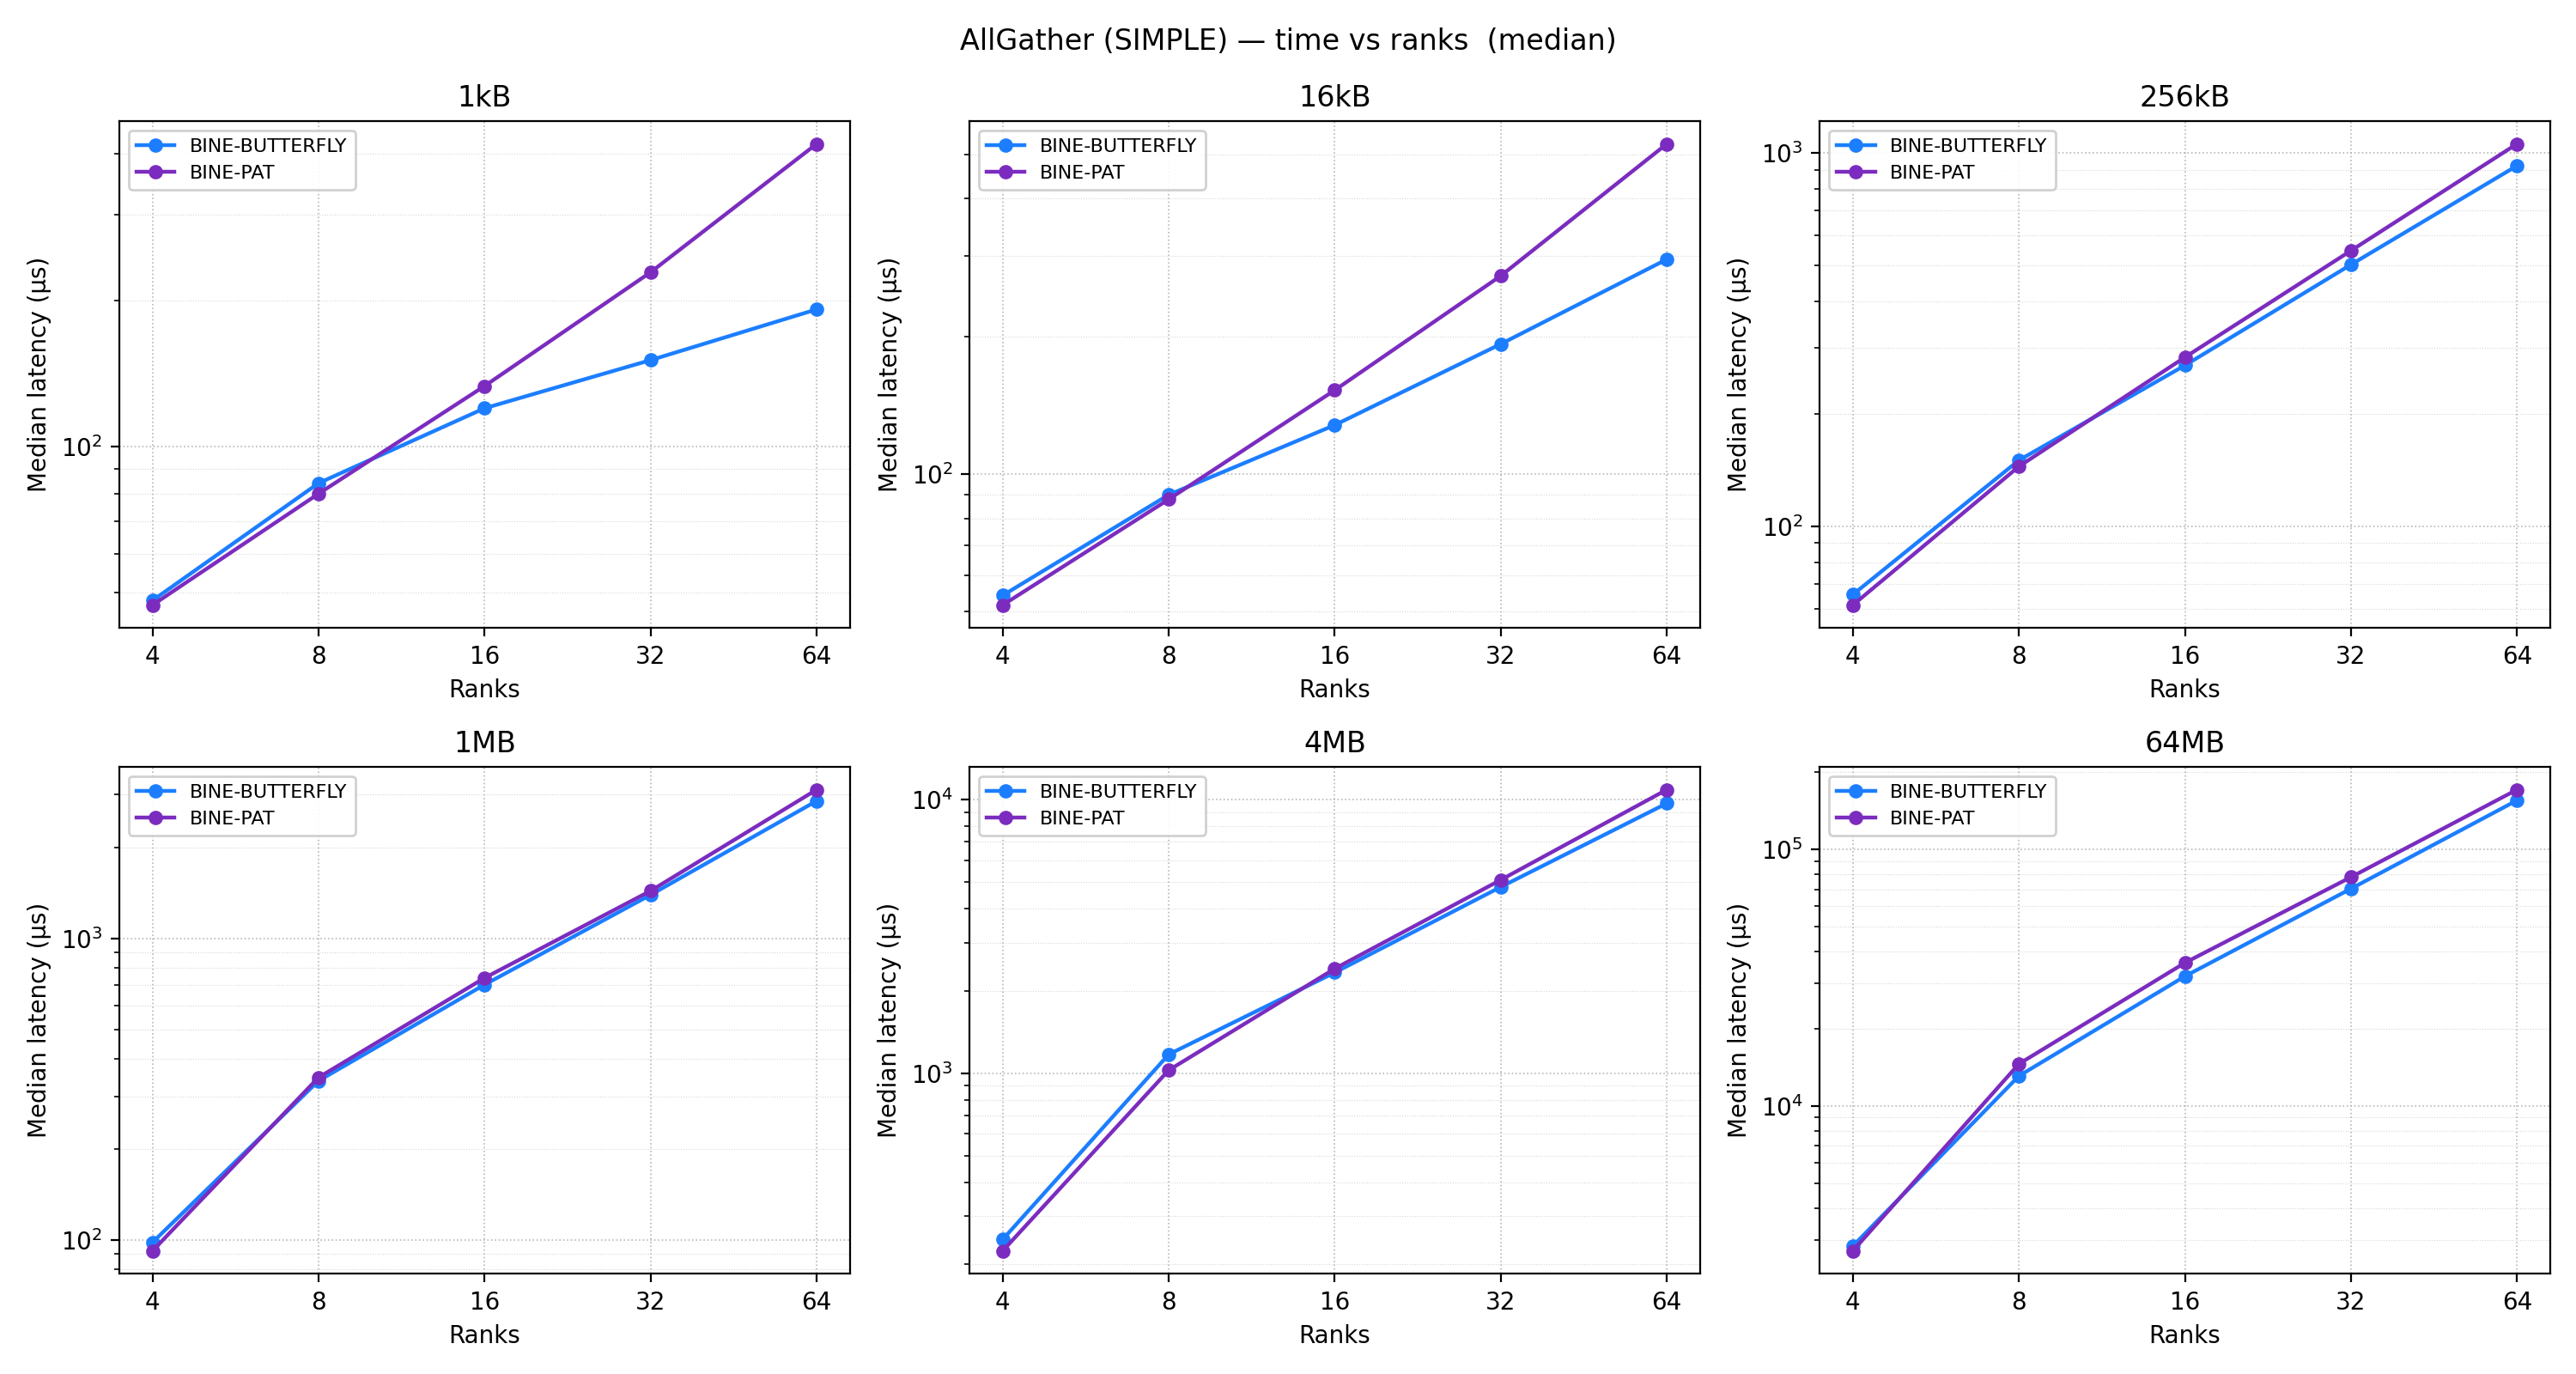
\includegraphics[width=0.92\linewidth]{AllGather_SIMPLE_vs_ranks_by_size_BINE_bm-best.png}
  \caption{Allgather with \texttt{SIMPLE}: median latency versus number of ranks, \bine{} butterfly (blue) against \bine{}-\pat{} (purple), each with its best strategy, for six block sizes. Both axes are logarithmic.}
  \label{fig:pat-scaling}
\end{figure}

\begin{table}[!htbp]
\centering
\small
\setlength{\tabcolsep}{4pt}
\renewcommand{\arraystretch}{1.1}
\sisetup{table-format=1.2, detect-weight=true, mode=text}
\caption{Median latency of \bine{}-\pat{} divided by that of the \bine{} butterfly, allgather with \texttt{SIMPLE}: same strategy (block-by-block, slice mode in both) and best strategy of each implementation. A value below $1$ means that \bine{}-\pat{} is faster. These values are in bold.}
\label{tab:pat-vs-bfly}
\begin{tabular}{@{}l *{5}{S} @{\hspace{2em}} *{5}{S}@{}}
\toprule
 & \multicolumn{5}{c}{Block-by-block} & \multicolumn{5}{c}{Best strategy} \\
\cmidrule(lr){2-6}\cmidrule(l){7-11}
Block size & {$p{=}4$} & {8} & {16} & {32} & {64} & {$p{=}4$} & {8} & {16} & {32} & {64} \\
\midrule
1\,kB   & {\bfseries 0.94} & {\bfseries 0.94} & {\bfseries 0.99} & 1.07 & {\bfseries 0.71} & {\bfseries 0.98} & {\bfseries 0.95} & 1.11 & 1.52 & 2.19 \\
16\,kB  & {\bfseries 0.94} & {\bfseries 0.98} & 1.19 & 1.41 & 1.71 & {\bfseries 0.95} & {\bfseries 0.98} & 1.19 & 1.41 & 1.79 \\
256\,kB & {\bfseries 0.94} & {\bfseries 0.96} & 1.05 & 1.09 & 1.14 & {\bfseries 0.94} & {\bfseries 0.96} & 1.05 & 1.09 & 1.14 \\
1\,MB   & {\bfseries 0.94} & 1.03 & 1.05 & 1.03 & 1.09 & {\bfseries 0.94} & 1.03 & 1.05 & 1.03 & 1.09 \\
4\,MB   & {\bfseries 0.91} & {\bfseries 0.88} & 1.03 & 1.06 & 1.12 & {\bfseries 0.91} & {\bfseries 0.88} & 1.03 & 1.06 & 1.12 \\
64\,MB  & {\bfseries 0.95} & 1.11 & 1.13 & 1.11 & 1.10 & {\bfseries 0.96} & 1.11 & 1.13 & 1.11 & 1.10 \\
\bottomrule
\end{tabular}
\end{table}

The aggregation does not deliver the gain expected in \cref{sec:pat-motivation}.
\bine{}-\pat{} is faster than the butterfly only with few ranks, by $2$--$12\,\%$ (on $4$ ranks at every size, on $8$ ranks at four of the six sizes), and from $16$ ranks on it is slower at every size: by $3$--$14\,\%$ from 256\,kB on, and by much more for small blocks, up to $2.2\times$ at 1\,kB on $64$ ranks.
The gap at small sizes is not a matter of strategy: the best strategy of \bine{}-\pat{} is block-by-block almost everywhere, and against the same strategy of the butterfly it is still $1.2$--$1.7\times$ slower at 16\,kB from $16$ ranks on (\cref{tab:pat-vs-bfly}).
The only point where \bine{}-\pat{} wins clearly, block-by-block at 1\,kB on $64$ ranks ($0.71$), is the irregular block-by-block point of the butterfly noted in \cref{sec:bfly-res-modes}.

\paragraph{Small blocks: the cost of an operation.}
The solid purple lines of \cref{fig:pat-scaling} show that for small blocks the latency of \bine{}-\pat{} is linear in $p$, not logarithmic.
At 1\,kB it grows from $47$ to $435$\,\textmu s between $4$ and $64$ ranks, by $6$--$8$\,\textmu s per added rank at every doubling (at 16\,kB by $7$--$9$\,\textmu s), close to the $8$--$11$\,\textmu s of the ring with \texttt{SIMPLE}. The butterfly with send in pos mode adds about $1.3$\,\textmu s per rank between $32$ and $64$ ranks.
The number of network transfers is not the cause: at these sizes $P$ is large, every step fits in one slot, and a channel posts $s$ messages (\cref{sec:pat-geom}).
What remains linear is the number of operations: a channel moves $n_c(p-1)$ pieces in the butterfly, and each of them is one send and one receive, i.e., $2(p-1)$ entries of the ring for a single chunk, each executed by the workers in order, with a \texttt{patBarrier} and the polling of the ring (\cref{alg:pat-kernel}).
The aggregation removes the empty FIFO steps of \cref{fig:bfly-slots}, but not the per-piece work on the device, and with a single group of workers the latter is serialised.
The butterfly kernels of block-by-block also issue one call per block, but send and receive progress in two groups of threads (\cref{sec:bfly-kernels}), so the two halves of the work overlap. This is consistent with the per-rank cost of block-by-block at 16\,kB being about twice as large in \bine{}-\pat{} ($7$--$9$\,\textmu s) as in the butterfly ($3.6$--$4.7$\,\textmu s, between $8$ and $64$ ranks).

Two changes would reduce this cost, both available in the native \pat{}.
The first is a parallel factor larger than one, i.e., several groups of workers executing independent operations (\cref{sec:pat-kernel}). The second is to keep a received piece in the slot and forward it from there, as \pat{} does (\cref{tab:pat-vs-bine}): in the butterfly the half received at a step is part of the window sent at the next one, so its receive and its send could be one operation, which would remove the extra copy and part of the operations.

\paragraph{Large blocks.}
From 256\,kB on the two implementations are within $15\,\%$, with \bine{}-\pat{} slower by $3$--$14\,\%$ from $16$ ranks on.
With large blocks the pieces are full chunks in both implementations ($P=1$, \cref{sec:pat-geom}), so the aggregation has nothing to save, and \bine{}-\pat{} keeps the costs of \cref{sec:pat-prims}: one more local copy per received piece and sends and receives alternated slot by slot in the same threads, which limits the slots in flight on a connection.
On $4$ ranks \bine{}-\pat{} is instead $4$--$9\,\%$ faster at every size, and on $8$ ranks it is faster up to 256\,kB and at 4\,MB.
With few ranks the steps are few and short, and the setup that the butterfly repeats at every step (two \texttt{Primitives} objects and a barrier of the whole block, \cref{sec:pat-motivation}) weighs more. \bine{}-\pat{} builds its primitives once per kernel.

%------------------------------------------------------------------------------
\FloatBarrier
\subsection{The four strategies}\label{sec:pat-res-modes}

\Cref{fig:pat-modes} shows the fastest strategy of either implementation at each point, and \cref{tab:pat-modes} the cost of the strategies relative to block-by-block on $64$ ranks, for both implementations.

\begin{figure}[!tbp]
  \centering
  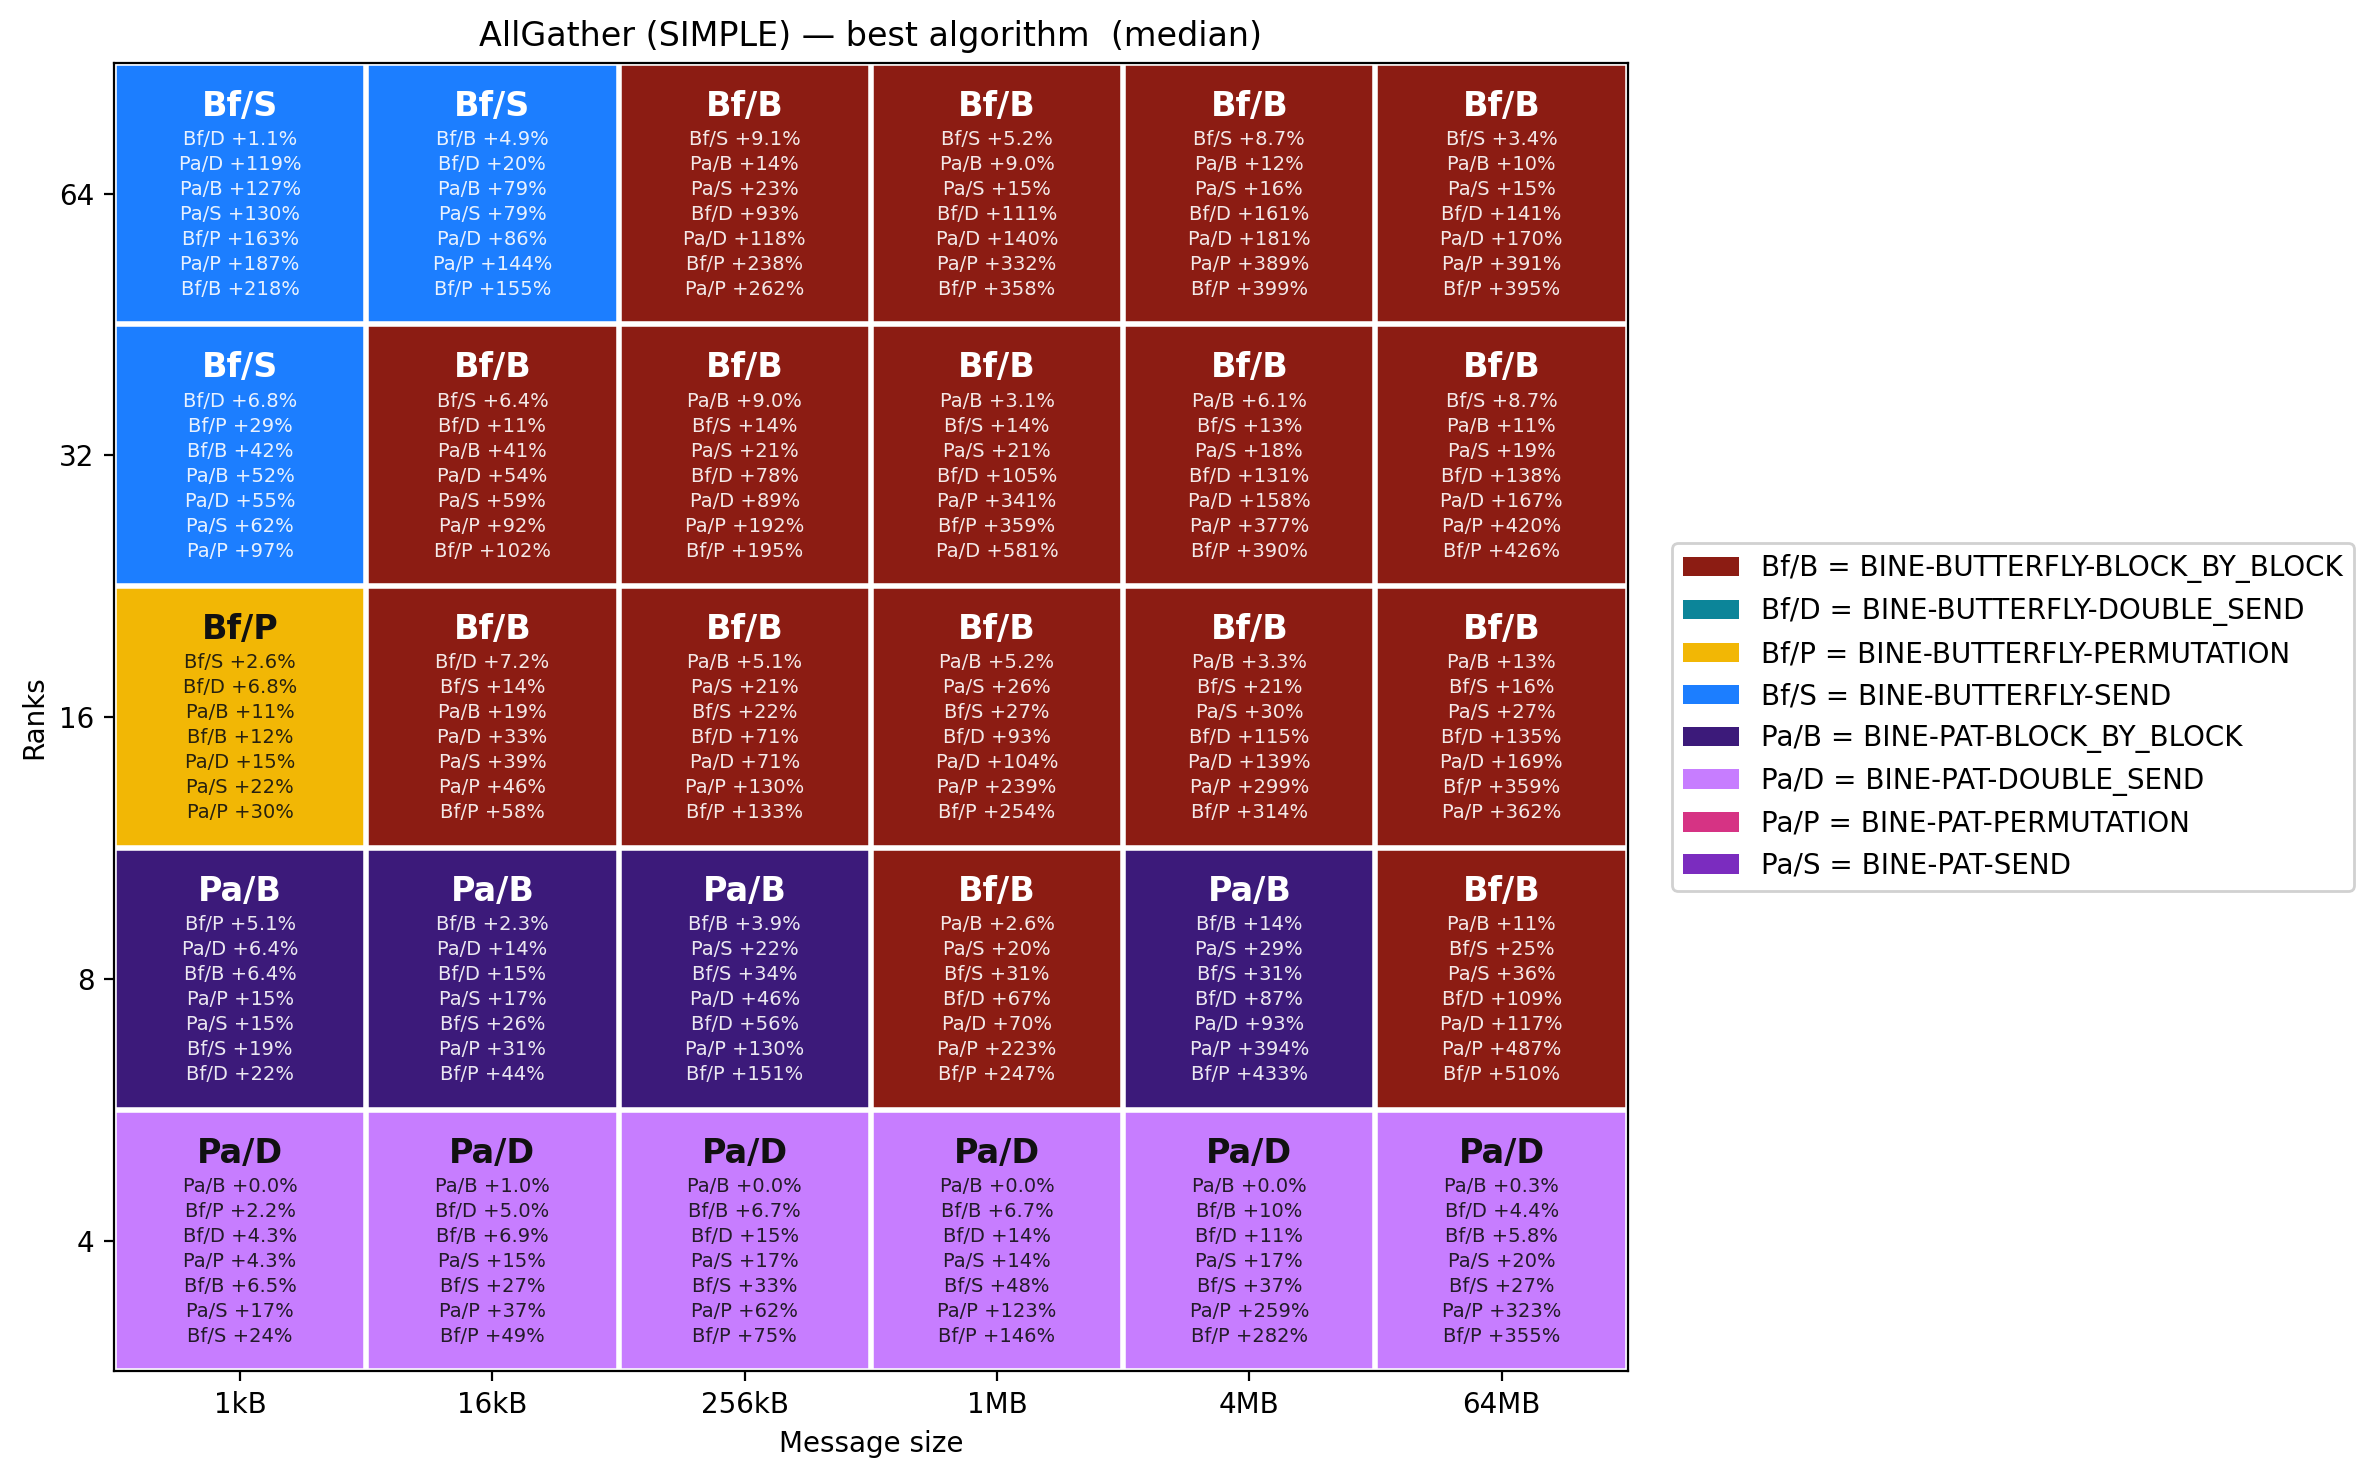
\includegraphics[width=0.73\linewidth]{AllGather_SIMPLE_best_algo_heatmap_BINE.png}
  \caption{Allgather with \texttt{SIMPLE}: fastest \bine{} implementation and strategy for each block size and number of ranks (median latency), without the ring. Each cell lists the other combinations with the percentage by which they are slower. Bf: \bine{} butterfly, Pa: \bine{}-\pat{}. B, S, P, D: block-by-block, send, permute and double send.}
  \label{fig:pat-modes}
\end{figure}

\begin{table}[htbp]
\centering
\small
\setlength{\tabcolsep}{4pt}
\renewcommand{\arraystretch}{1.1}
\sisetup{table-format=1.2, detect-weight=true, mode=text}
\caption{Latency of send, double send and permute relative to block-by-block of the same implementation, allgather with \texttt{SIMPLE} on $64$ ranks (a value below $1$ means faster than block-by-block). The butterfly columns are those of \cref{tab:bfly-modes}.}
\label{tab:pat-modes}
\begin{tabular}{@{}l *{3}{S} @{\hspace{2em}} *{3}{S}@{}}
\toprule
 & \multicolumn{3}{c}{\bine{}-\pat{}} & \multicolumn{3}{c}{\bine{} butterfly} \\
\cmidrule(lr){2-4}\cmidrule(l){5-7}
Block size & {send} & {double} & {permute} & {send} & {double} & {permute} \\
\midrule
1\,kB   & 1.01 & 0.97 & 1.26 & 0.31 & 0.32 & 0.83 \\
16\,kB  & 1.00 & 1.04 & 1.37 & 0.95 & 1.15 & 2.43 \\
256\,kB & 1.08 & 1.91 & 3.16 & 1.09 & 1.93 & 3.38 \\
1\,MB   & 1.06 & 2.20 & 3.97 & 1.05 & 2.11 & 4.58 \\
4\,MB   & 1.04 & 2.51 & 4.36 & 1.09 & 2.61 & 4.99 \\
64\,MB  & 1.04 & 2.45 & 4.46 & 1.03 & 2.41 & 4.95 \\
\bottomrule
\end{tabular}
\end{table}

In \bine{}-\pat{} the four strategies differ only in the pre-step, the order of the pieces and the post-step (\cref{tab:pat-strategies}). Every strategy runs in slice mode and every piece is packed in a slot, so the data layout no longer changes the number of transfers.
Below 16\,kB the four strategies are therefore within $1$--$37\,\%$ of one another, and send and double send lose the advantage of $3\times$ they have in the butterfly at 1\,kB, which came from pos mode and not from the strategy (\cref{sec:bfly-res-modes}).
Block-by-block, which has neither a pre-step nor a post-step, is the best or within $3\,\%$ of the best at every point.

The extra costs of the other strategies are those of the butterfly.
Send pays the exchange of the pre-step, $10$--$29\,\%$ on $4$ to $16$ ranks and $1$--$8\,\%$ on $64$, since it moves one block against the $p-1$ of the butterfly.
Permute pays the in-place permutation of the whole output buffer (\cref{sec:pat-permute}), $4$--$4.5\times$ the time of block-by-block from 1\,MB on, at $64$ ranks. In absolute terms it takes within $9\,\%$ of the time of permute in the butterfly from 16\,kB on, so restricting the permutation to the slice of each channel neither helps nor hurts noticeably.

\paragraph{Double send.}
Double send is $1.9$--$2.5\times$ slower than block-by-block from 256\,kB on, as in the butterfly (\cref{sec:bfly-res-modes}).
\Cref{sec:bfly-res-modes} attributes this to the schedule: the distance-halving schedule sends its largest windows to the farthest partners, which are on other nodes, and moves $2$--$2.6\times$ as many blocks over the network as the distance-doubling one (\cref{fig:bfly-dh-tree,tab:bfly-internode}).
\bine{}-\pat{} shares only the schedule with the butterfly kernels, and shows the same pattern: on $4$ ranks, all on NVLink, double send and block-by-block take the same time at every size (ratio $1.00$), and at 64\,MB the ratio is $1.95$, $2.38$, $2.41$ and $2.45$ on $8$, $16$, $32$ and $64$ ranks, against the $2.00$, $2.40$, $2.55$ and $2.61$ of the inter-node traffic and the $2.09$, $2.35$, $2.38$ and $2.41$ of the butterfly.
This confirms that the cause is in the schedule and not in the kernels.

%------------------------------------------------------------------------------
\FloatBarrier
\subsection{Comparison with the ring}\label{sec:pat-res-ring}

\Cref{fig:pat-heatmap-ring} adds the ring with both protocols and the butterfly with \texttt{LL}.
With \texttt{SIMPLE} on both sides \bine{}-\pat{} is faster than the ring for small blocks on many ranks: by $1.09$--$1.32\times$ at 1\,kB from $16$ ranks on and by $1.09$--$1.18\times$ at 16\,kB from $8$ ranks on, against up to $2.9\times$ for the butterfly (\cref{sec:bfly-res-ring}), since its latency is linear in $p$ like that of the ring.
From 1\,MB on it is $1.3$--$2.2\times$ slower than the ring, slightly more than the butterfly.
\bine{}-\pat{} has no \texttt{LL} variant, and the ring with \texttt{LL} is $2.3$--$3.3\times$ faster than it at 1\,kB and 16\,kB, so it is never the fastest algorithm in \cref{fig:pat-heatmap-ring}.

\begin{figure}[!tbp]
  \centering
  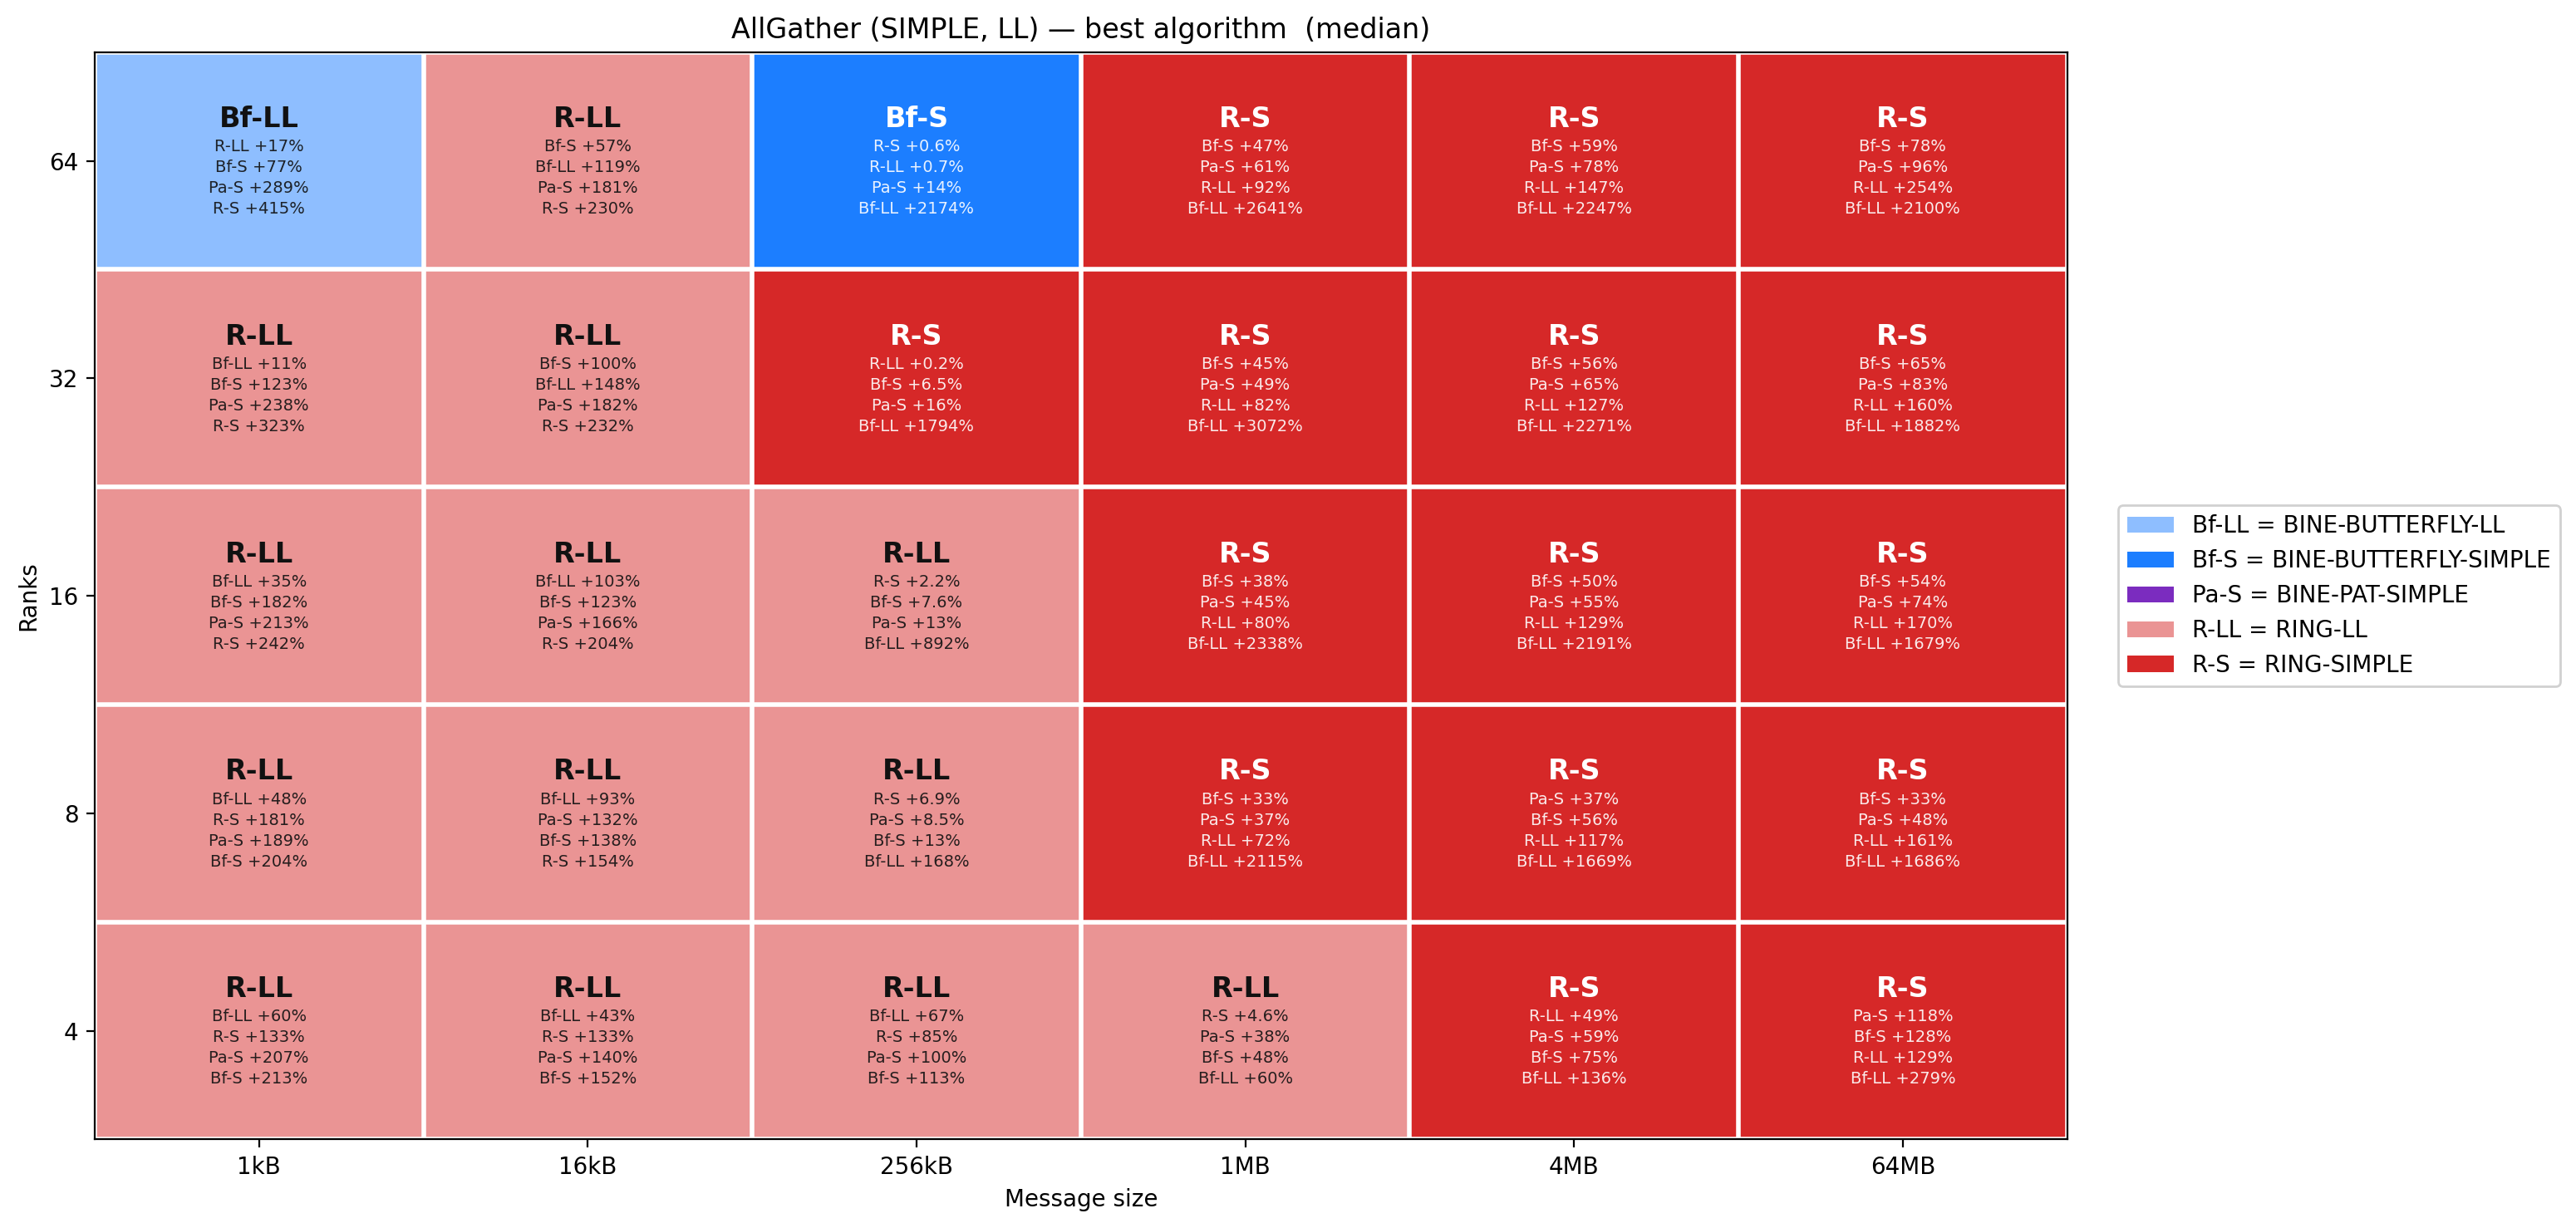
\includegraphics[width=0.95\linewidth]{AllGather_SIMPLE+LL_best_algo_heatmap_bm-best.png}
  \caption{Allgather: fastest algorithm and protocol for each block size and number of ranks (median latency), each \bine{} implementation with its best strategy. Each cell lists the other combinations with the percentage by which they are slower. Bf: \bine{} butterfly, Pa: \bine{}-\pat{}, R: \nccl{} ring. The suffixes S and LL are the protocols.}
  \label{fig:pat-heatmap-ring}
\end{figure}

\subsection{Comparison with the native PAT}\label{sec:pat-res-native}

The native \pat{} allgather runs only with one rank per node (\cref{sec:nccl-pat}), so it cannot be compared on the configuration above, where each node hosts four ranks.
We compare it with \bine{}-\pat{} and with the ring on a separate set of runs with one rank per node.

\paragraph{Setup.}
These runs use the MeluXina supercomputer, the system of \cref{ch:tree}, with nodes of four NVIDIA A100 GPUs, of which only one is used: $p\in\{4,8,16\}$ ranks on as many nodes, so every transfer crosses the network and NVLink is not used.
Sizes, iterations and statistics are those of the runs above (1\,kB to 64\,MB per block, $10$ warmup and $40$ measured iterations, median latency).
The native \pat{} exists only for \texttt{SIMPLE}, so the comparison is with \texttt{SIMPLE}, and the ring is also given with \texttt{LL}.
The butterfly kernels of \cref{ch:butterfly} were not run in this configuration.
Since the system is not the same, the absolute times are not comparable with those of the previous sections.

\Cref{fig:pat-native-scaling} shows the latency of the three algorithms, \bine{}-\pat{} with its best strategy, and \cref{fig:pat-native-heatmap} the fastest of them at each point, with the percentage by which the others are slower.

\begin{figure}[!tbp]
  \centering
  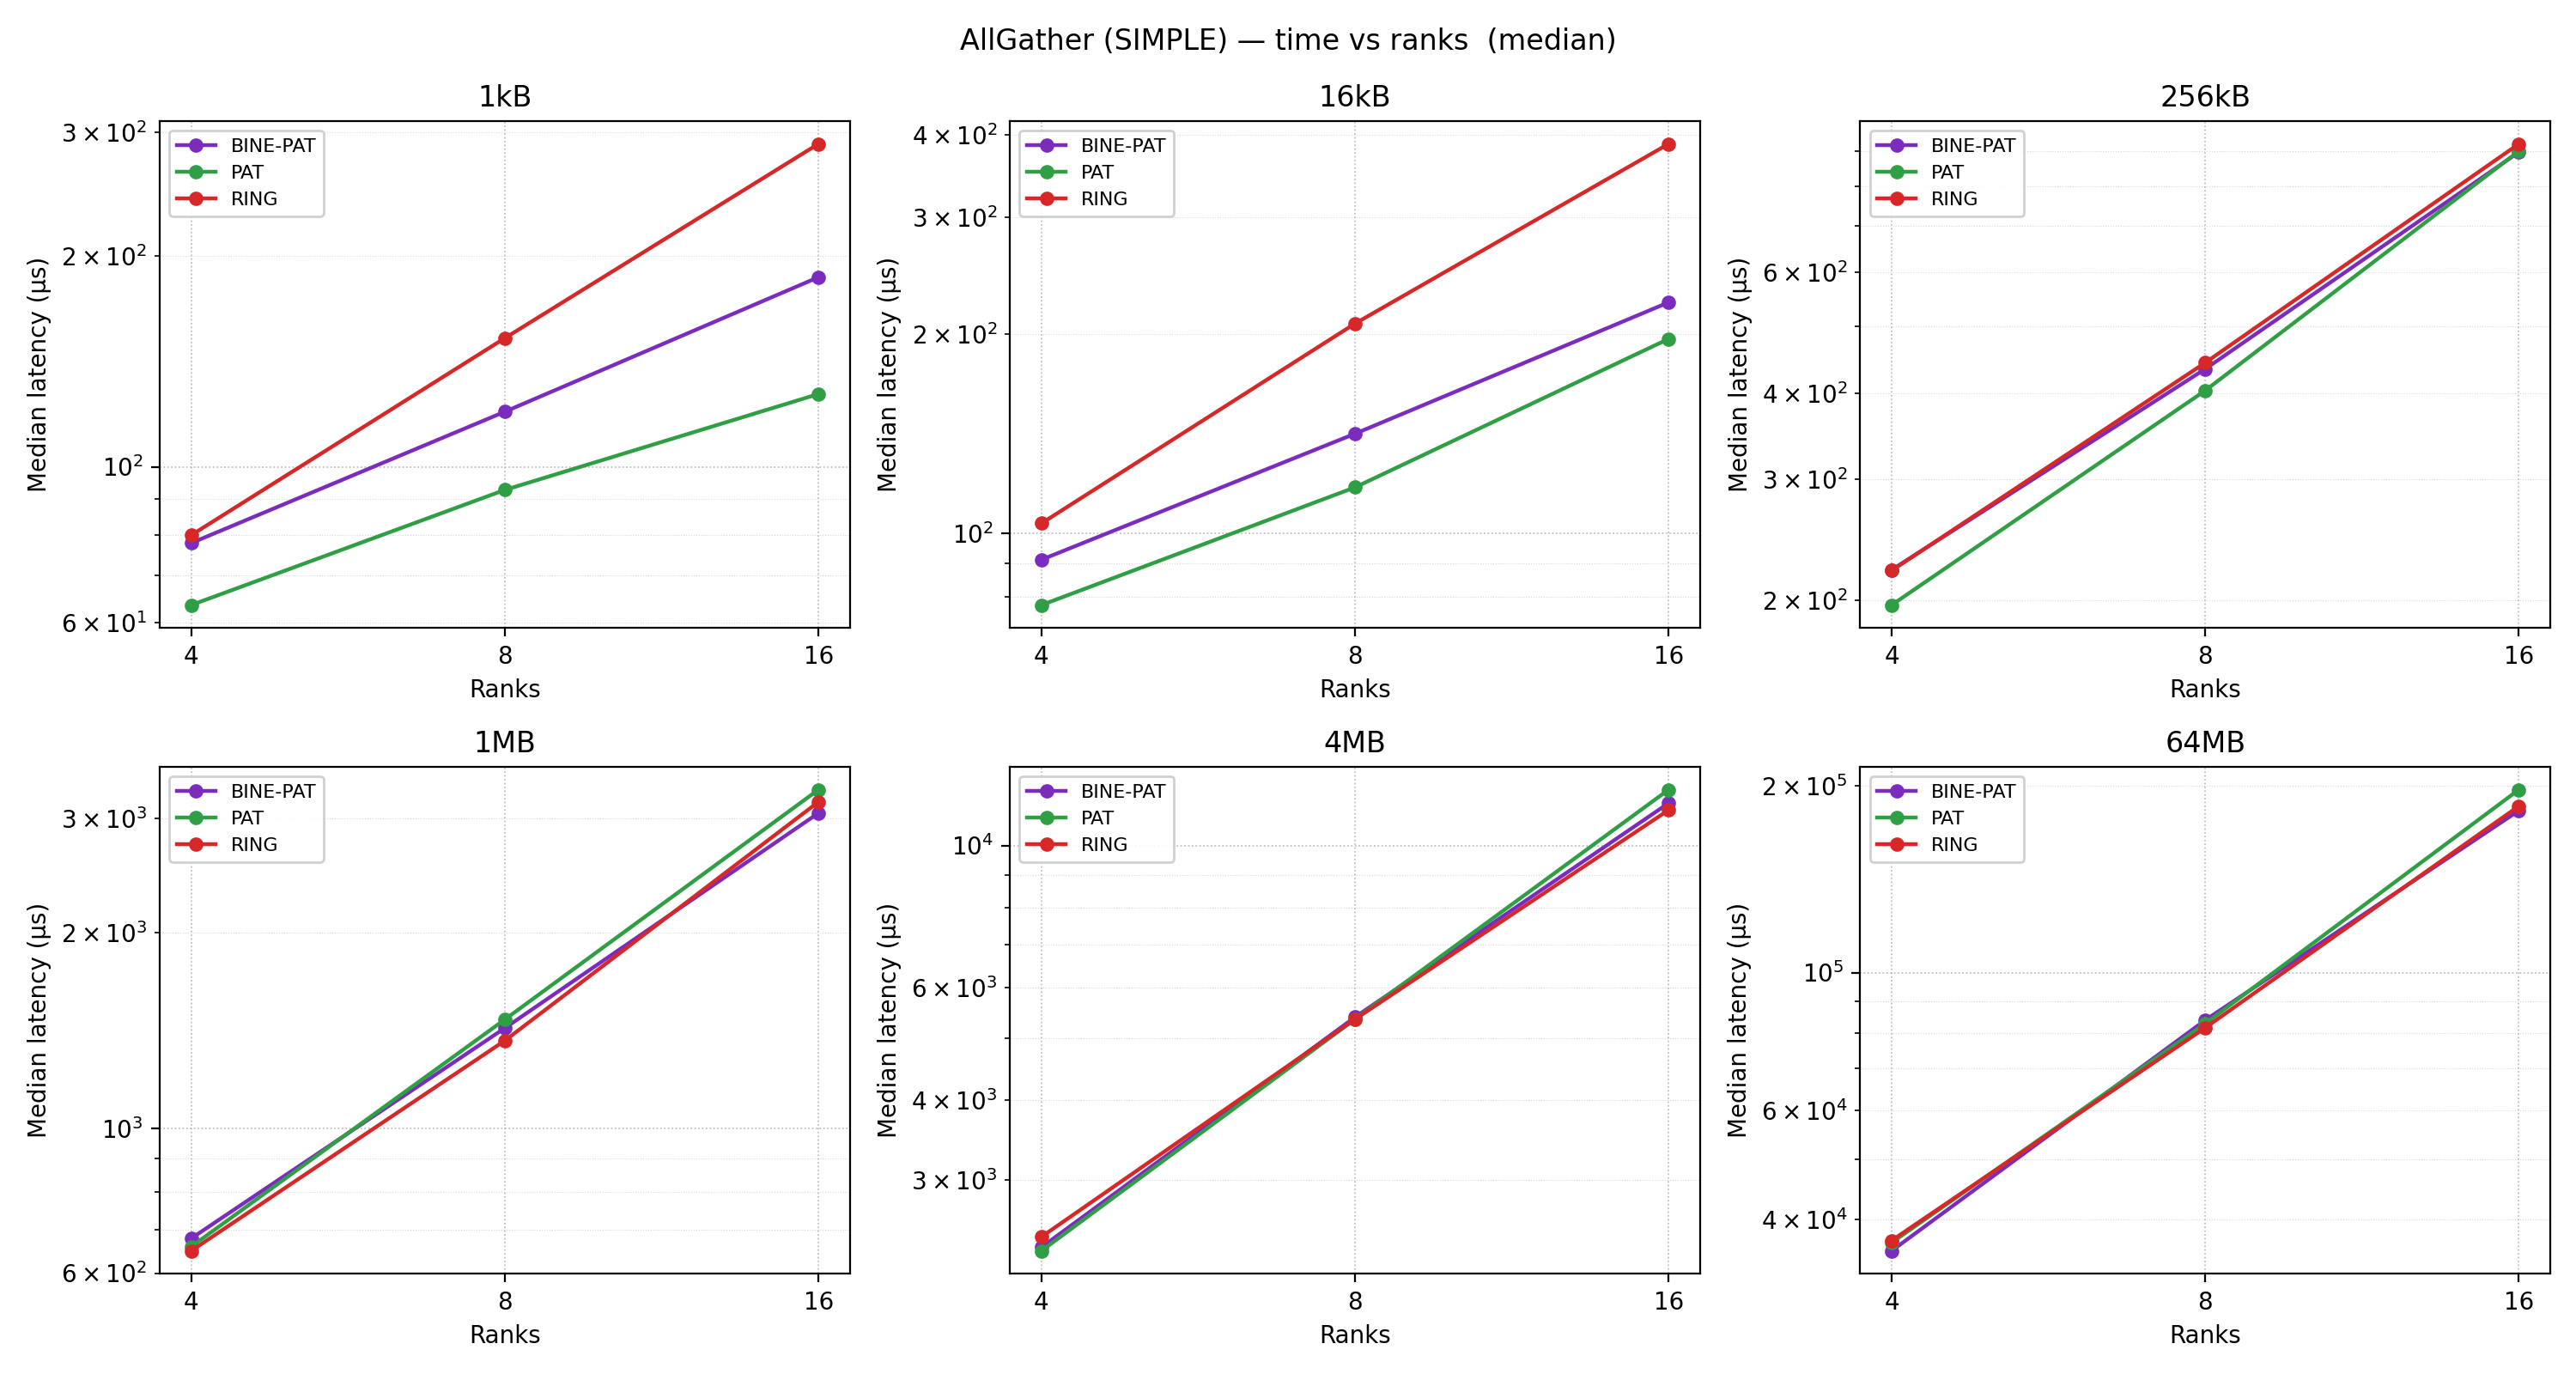
\includegraphics[width=0.92\linewidth]{AllGather_SIMPLE_vs_ranks_by_size_PAT-1ppn.png}
  \caption{Allgather with \texttt{SIMPLE} and one rank per node (MeluXina): median latency versus number of ranks, \bine{}-\pat{} with its best strategy (purple), native \pat{} (green) and \nccl{} ring (red), for six block sizes. Both axes are logarithmic.}
  \label{fig:pat-native-scaling}
\end{figure}

\begin{figure}[!tbp]
  \centering
  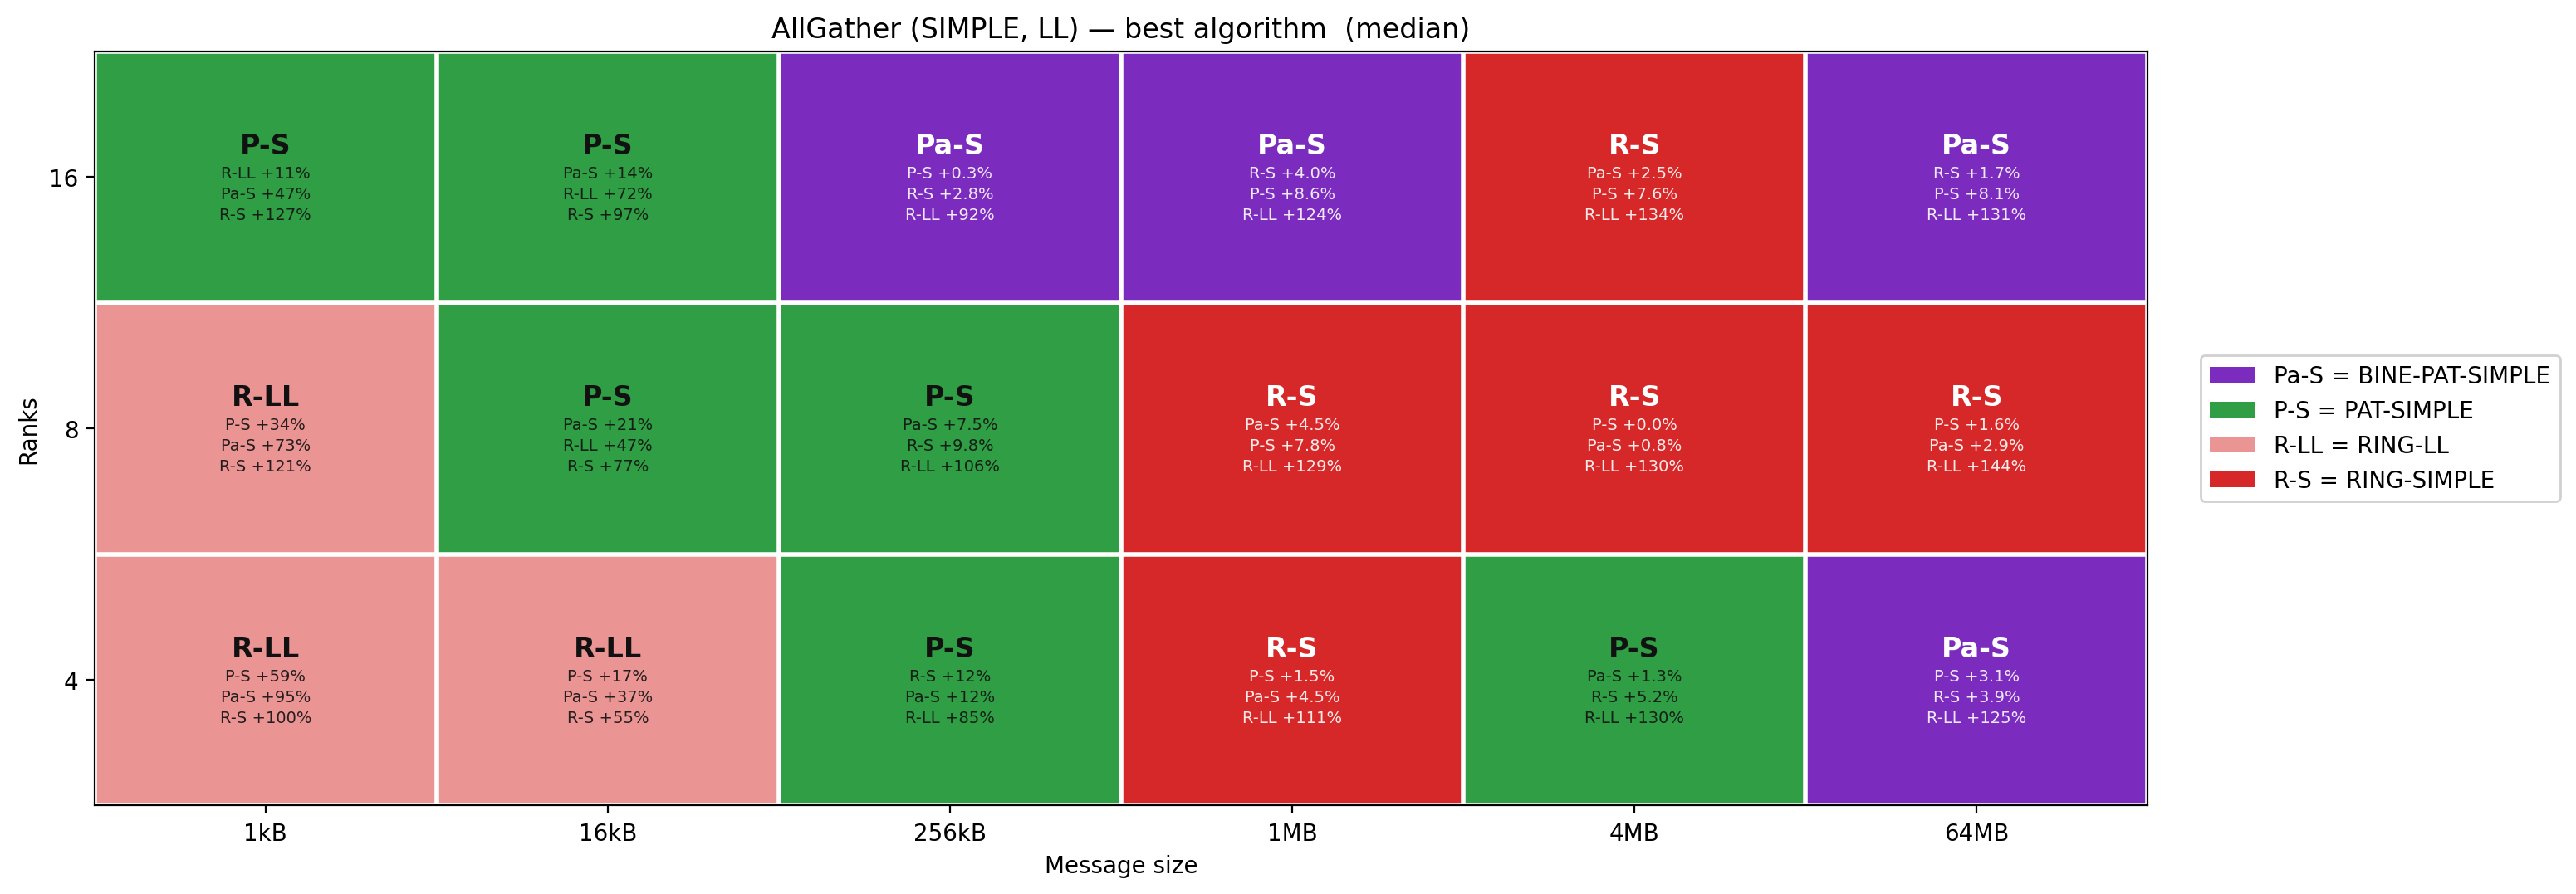
\includegraphics[width=\linewidth]{AllGather_SIMPLE+LL_best_algo_heatmap_PAT-1ppn.png}
  \caption{Allgather with one rank per node (MeluXina): fastest algorithm and protocol for each block size and number of ranks (median latency), \bine{}-\pat{} with its best strategy. Each cell lists the other combinations with the percentage by which they are slower. Pa-S: \bine{}-\pat{}, P-S: native \pat{}, R-S and R-LL: \nccl{} ring with \texttt{SIMPLE} and with \texttt{LL}.}
  \label{fig:pat-native-heatmap}
\end{figure}

\paragraph{Small blocks.}
Up to 16\,kB the native \pat{} is the fastest algorithm with \texttt{SIMPLE}, and \bine{}-\pat{} is $1.14$--$1.47\times$ slower.
At 1\,kB the gap grows with $p$: the native \pat{} goes from $64$ to $127$\,\textmu s between $4$ and $16$ ranks, about $7$ and $4$\,\textmu s per added rank, while \bine{}-\pat{} goes from $78$ to $186$\,\textmu s, about $11$ and $8$\,\textmu s per added rank.
This is the per-operation cost of \cref{sec:pat-res-bfly}, now measured against the same machinery: the two kernels share the ring of descriptors, the workers and \texttt{patCopy}, and differ in the schedule and in the two features that \bine{}-\pat{} lacks.
The native \pat{} keeps the received data in the slot and forwards it in the same operation, and runs several groups of workers in parallel, while in \bine{}-\pat{} every piece is a separate send and receive executed by one group (\cref{tab:pat-vs-bine}).
The gap at small sizes therefore comes from the execution and not from the schedule.
Both are still much faster than the ring with \texttt{SIMPLE}, whose latency is linear in $p$ with a larger slope ($18$\,\textmu s per added rank at 1\,kB): at $16$ ranks \bine{}-\pat{} is $1.55\times$ faster at 1\,kB and $1.74\times$ at 16\,kB.
The ring with \texttt{LL} is the fastest at 1\,kB on $4$ and $8$ ranks, but at $16$ ranks the native \pat{} overtakes it at 1\,kB, and both \pat{} implementations are faster than it at 16\,kB from $8$ ranks on (\bine{}-\pat{} by $1.22$ and $1.51\times$).

\paragraph{Large blocks.}
From 256\,kB on the three algorithms with \texttt{SIMPLE} are within $12\,\%$ of one another, and from 1\,MB within $8\,\%$. The ring with \texttt{LL} is $1.6$--$2.3\times$ slower than with \texttt{SIMPLE}.
With one rank per node every transfer crosses the network, which is the bottleneck, and the three move the same volume, $\tfrac{p-1}{p}n$ per rank.
\bine{}-\pat{} is $5$--$8\,\%$ faster than the native \pat{} on $16$ ranks from 1\,MB on.
This is consistent with the shorter distances of the \bine{} schedule (\cref{sec:bg-bine-butterfly}), which matter on a network whose cost depends on the distance between nodes.

\paragraph{Strategies.}
The strategies keep the ordering of the configuration with four ranks per node, with one exception.
Send pays its pre-step ($1.02$--$1.33\times$ block-by-block, decreasing with $p$) and permute its permutation ($1.9$--$2.4\times$ from 1\,MB on).
Double send, instead, takes the same time as block-by-block at every point ($0.96$--$1.01\times$) and is the best strategy at $11$ of the $18$ points.
With one rank per node all partners are on other nodes, so the distance-halving schedule no longer moves more data over the network than the distance-doubling one, and its slowdown disappears.
This is the counterpart of the measurement on $4$ ranks with four ranks per node, where all partners were on NVLink, and confirms that the slowdown of double send in \cref{sec:pat-res-modes,sec:bfly-res-modes} comes from the hierarchy of the system (\cref{tab:bfly-internode}).

\subsection{Summary}

Executing the \bine{} allgather on the \pat{} machinery removes the dependence of the transfers on the data layout: the four strategies issue the same messages, and block-by-block, the simplest, is the best one.
It does not make the allgather faster.
\bine{}-\pat{} is up to $12\,\%$ faster than the butterfly kernels on $4$ and, at some sizes, $8$ ranks, but from $16$ ranks on it is $3$--$14\,\%$ slower for large blocks and up to $2.2\times$ slower for small ones, where its latency grows linearly with $p$: the aggregation reduces the network messages to $s$ per channel, but each piece is still an operation on the device, executed in order by a single group of workers.
With one rank per node the native \pat{} is $1.14$--$1.47\times$ faster than \bine{}-\pat{} up to 16\,kB, with the same machinery, which points to the two features that \bine{}-\pat{} lacks, a parallel factor larger than one and a fused receive-and-forward, as the natural next steps. For large blocks the two are within $8\,\%$, with \bine{}-\pat{} slightly ahead on $16$ ranks.
The measurements also explain the slowdown of double send in both implementations: the distance-halving schedule sends its largest windows to the farthest partners, which are on other nodes, and moves $2$--$2.6\times$ as much data over the network as the distance-doubling one. With one rank per node, where all partners are on other nodes, the slowdown disappears.

% Uses the macros of the preamble (\nccl, \bine, \pat, \todo, \Send, \Recv, \none, \rtn, \ntr, \bigO,
% \binepic, \blab, and the colors ch0, ch1, chunkA, chunkB, chunkC, crosslink).
% It also defines \binerot below; it can be moved to the preamble.

% \bine{} tree of $8$ ranks rooted at t (labels = (relative rank + t) mod 8); the root is highlighted.
\newcommand{\binerot}[2]{%
  \begin{tikzpicture}[baseline=(lab.north), x=0.85cm, y=0.75cm,
      rank/.style={circle, draw, minimum size=0.55cm, inner sep=0pt,
                   fill=white, font=\scriptsize},
      e/.style={-{Stealth[length=2mm]}, line width=1.2pt, black!45,
                shorten >=1pt, shorten <=1pt}]
    \useasboundingbox (-1.8,0.5) rectangle (2.7,-4.5);
    \foreach \i/\px/\py in {0/0.7/0, 3/-0.6/-1.1, 7/0.9/-1.1, 1/2.1/-1.1,
                            4/-1.3/-2.2, 2/-0.1/-2.2, 6/0.9/-2.2, 5/-1.3/-3.3} {
      \pgfmathtruncatemacro{\rk}{mod(\i+#1,8)}
      \node[rank] (n\i) at (\px,\py) {\rk};
    }
    \foreach \a/\b in {0/3,0/7,0/1,3/4,3/2,7/6,4/5} \draw[e] (n\a) -- (n\b);
    \pgfmathtruncatemacro{\rt}{mod(#1,8)}
    \node[rank, draw=crosslink, fill=crosslink!20, thick] at (n0) {\rt};
    \node[font=\footnotesize, align=center] (lab) at (0.45,-4.1) {#2};
  \end{tikzpicture}%
}

\chapter{Tree-Based Allreduce}\label{ch:treeallreduce}
This chapter implements the allreduce of \bine{} in \nccl{} as a reduce followed by a broadcast on the same \bine{} tree, executed by a single kernel.
It reuses the tables of \cref{ch:tree} and the structure of the \nccl{} tree allreduce (\cref{sec:nccl-tree}).
\Cref{sec:tar-motivation} explains why this algorithm is a good fit for \nccl{}, \cref{sec:tar-schedule} how the tree is chosen for each channel, and \cref{sec:tar-kernel} how the kernel works.
%==============================================================================
\section{Motivation}\label{sec:tar-motivation}
\paragraph{The allreduce of the butterfly.}
For large vectors, the allreduce of \bine{} is a reduce-scatter followed by an allgather on the \bine{} butterfly, and for small vectors a recursive doubling in which the whole vector is exchanged at every step~\cite{desensi2025bine}.
Both follow the schedule of \cref{ch:butterfly}.
In a butterfly each step moves a different amount of data, with a different partner: the window that a rank sends is half of the previous one in the reduce-scatter and twice as large in the allgather.
\nccl{} is organised differently.
The work is split among the channels once, by the host, before the kernel starts (\cref{sec:nccl-cbd}), and the connections of a channel are fixed at the creation of the communicator (\cref{sec:nccl-channels}). \nccl{} does not repartition the data among the channels from one step to the next.
A channel works on a fixed slice of the vector, so the blocks of a window are either cut in slices that are spread in the buffer, and are sent as many small pieces, or are assigned whole to the channels by a second partition (the \emph{slice} and \emph{pos} modes of \cref{sec:bfly-pos}), which is valid only for some strategies.
\Cref{ch:pat} goes around the same constraint in a different way, by aggregating the pieces in the slots of the FIFO with the machinery of \pat{} (\cref{sec:pat-motivation}).
Both solutions add machinery for the non-contiguous data, which is the cost of an algorithm in which the size of the transfers changes at every step.
\paragraph{The tree.}
The broadcast and the reduce of \cref{ch:tree} do not have this problem.
At every step in which a rank takes part, it sends or receives the \emph{whole} slice of its channel, and the same slice, in chunks, at each level of the tree.
The amount of data per edge is fixed, so the partition of \nccl{} fits without changes: no second partition, no permutation of the blocks, no staging buffer and no schedule thread.
An allreduce built as a reduce followed by a broadcast inherits this property.
The structure is shown in \cref{fig:tar-tree}: the reduce and the broadcast use the same edges, in opposite directions.
The composition is not one of the two allreduce algorithms of the \bine{} paper, which are based on the butterfly (Sec.~4.4 of~\cite{desensi2025bine}). It combines the reduce and the broadcast for small vectors that the paper defines on the distance-halving \bine{} tree (Sec.~4.5 of~\cite{desensi2025bine}), and the allreduce as a reduce followed by a broadcast is the one of \cref{sec:bg-collectives}.
Rooting that same pattern differently on each channel, rather than once for the whole communicator, is what maps it onto \nccl{}: the result is one root per channel instead of one per rank, at most $\min(p,\mathit{nchannels})$ of them, not a new algorithm.
\begin{figure}[t]
  \centering
  \binepic{reduce (leaves first)}{%
    \blab{5}{4}{1}{ch0}\blab{2}{3}{1}{ch0}\blab{6}{7}{1}{ch0}\blab{1}{0}{1}{ch0}%
    \blab{4}{3}{2}{ch0}\blab{7}{0}{2}{ch0}%
    \blab{3}{0}{3}{ch0}}\hfill
  \binepic{broadcast (root first)}{%
    \blab{0}{3}{1}{ch1}%
    \blab{0}{7}{2}{ch1}\blab{3}{4}{2}{ch1}%
    \blab{0}{1}{3}{ch1}\blab{3}{2}{3}{ch1}\blab{7}{6}{3}{ch1}\blab{4}{5}{3}{ch1}}
  \caption{The allreduce on the \bine{} tree rooted at rank $0$ ($p=8$): the reduce
           (left, blue) and the broadcast (right, orange) use the same edges in opposite
           directions. Each edge carries the same chunks of the same slice, and the
           numbers are the time slots of one chunk.}
  \label{fig:tar-tree}
\end{figure}
\paragraph{Cost.}
The tree has $s=\log_2p$ levels, the same shape as the binomial tree of \cref{sec:bg-bine}, but not the same cost model: \nccl{} pipelines the vector in chunks along the tree, as in \cref{sec:bg-double-tree}, so the latency term is not the $2s\,\alpha$ of the non-pipelined binomial tree of \cref{tab:bg-allreduce-cost}.
Since the \bine{} tree is a binomial tree and not a binary one, the root has $s$ children and sends each chunk $s$ times, so the bandwidth term of a channel remains $\bigO{s\,n\beta}$ (\cref{sec:tree-collectives}).
The number of children of the other ranks is smaller: $u(r)-1$ for rank $r$ (\cref{sec:tree-collectives}).
To avoid that the same rank has the largest fan-out in all the channels, the root of the tree is not fixed but depends on the channel (\cref{sec:tar-schedule}).
The combination of two complementary \bine{} trees, as in the double binary tree of \cref{sec:bg-double-tree}, is left as future work.
%==============================================================================
\section{Schedule}\label{sec:tar-schedule}
The peers are those of the \bine{} tree of \cref{sec:tree-impl}.
The root-$0$ tables $\Send$ and $\Recv$ are stored in \texttt{channel.bine}, and the tree rooted in $t\neq0$ is obtained by rotating the ranks by $t$ as in \cref{sec:tree-root}.
As in \cref{ch:tree}, the schedule is defined for $p=2^s$ ranks.
In the kernel, a rank obtains its place in the tree of its channel with
\begin{center}\small
\texttt{ncclBineArRoot}$(\mathit{channelId},p)\;\rightarrow\;t,$\\
\texttt{ncclBineArTreeNeighbors}$(\Send,\Recv,p,s,t,r)\;\rightarrow\;(\mathit{parent},\mathit{children},n_c).$
\end{center}
The first function gives the root of the tree used by the channel, and the second reads the tables and returns the parent of the rank, or $-1$ if it is the root, and its $n_c$ children, at most \texttt{BINE\_AR\_MAX\_FAN}.
By \cref{eq:recv-table,eq:send-table}, for the tree rooted in $t$ and the rank $r'=(r-t)\bmod p$ relative to the root, the parent is $\pi_{i_{r'}}(r')$ and the children are $\{\pi_i(r')\mid i_{r'}<i\le s-1\}$, rotated back by $t$.
A rank can then be the root, a leaf ($n_c=0$) or an internal rank of the tree, and the role changes from channel to channel, since the root does.
The root of channel $c$ is the bit reversal of $c \bmod p$ on $s$ bits (for $p=8$: $0,4,2,6,\dots$ for channels $0,1,2,3,\dots$), so that even the first few channels, when they are fewer than the ranks, have roots far apart and load different links, and for $p$ not a power of two it is $c\bmod p$.
\Cref{fig:tar-roots} shows the trees of the first channels.
\begin{figure}[t]
  \centering
  \binerot{0}{channel $0$, $t=0$}\hfill
  \binerot{4}{channel $1$, $t=4$}\hfill
  \binerot{2}{channel $2$, $t=2$}
  \caption{Tree of each channel for $p=8$. The root of channel $c$ (in red) is the bit
           reversal of $c$ on $s$ bits ($0,4,2,6,\dots$), and the tree is the one rooted
           in $0$ with the ranks rotated by $t$. Even the first channels have roots far
           apart, and the role of a rank (root, internal, leaf) changes from channel to
           channel.}
  \label{fig:tar-roots}
\end{figure}
The array of the children is padded with $-1$, which the \texttt{Primitives} take as the end of the peers, and its size, \texttt{BINE\_AR\_MAX\_FAN}, is fixed at compile time to $20$.
The root has $s$ children, so this covers up to $2^{20}$ ranks, far more than any communicator, and the larger fan has a negligible cost, since it only enlarges the array of the peers.
Since the connections of a channel are created at the creation of the communicator (\cref{sec:nccl-channels}), the setup has to create, for each channel, the connections towards the parent and towards all the children of the tree rooted in the root of that channel.
%==============================================================================
\section{Kernel}\label{sec:tar-kernel}
The kernel, \texttt{runBineTree}, follows the structure of the \nccl{} tree allreduce (\texttt{runTreeSplit}, \cref{sec:nccl-tree}).
It is a template on the protocol, and runs one block per channel.
\paragraph{Slice and roles.}
The block obtains its slice with \texttt{ncclCollCbdPart} (\cref{sec:nccl-cbd}) and returns at once if the slice is empty: a channel with no data does not take part in the operation, and the proxy registers no operation for it.
It then computes the root, the parent and the children as in \cref{sec:tar-schedule}.
If the rank has neither parent nor children, the communicator has a single rank, and the kernel only copies the slice from \texttt{sendbuff} to \texttt{recvbuff} when they differ.
\Cref{fig:tar-roles} shows the three roles that a rank can have.
\paragraph{Root.}
The root has no parent: for each chunk the reduce ends and the broadcast starts at the same rank.
All the threads of the block execute a single fused primitive, \texttt{recvReduceCopySend}, built with \texttt{FanSymmetric}$\langle\texttt{BINE\_AR\_MAX\_FAN}\rangle$ with the children as the peers on both sides: for each chunk, it receives the chunk from all the children, combines it with its own input, writes the result in \texttt{recvbuff} and sends it to all the children.
The post-operation of the reduction (for example, the division of the average) is applied here, once, by passing \texttt{postOp}$=$\texttt{true}.
\paragraph{Non-root ranks.}
The other ranks split the threads of the block in two groups, as \nccl{} does for its tree: with \texttt{Simple} the first half, plus $64$ threads when the half is at least $256$ threads, and with \texttt{LL} and \texttt{LL128} about $70\,\%$ of the threads, rounded to a whole number of warps, since receiving from several children is more expensive than sending to them.
\begin{itemize}
  \item The \emph{reduce} group, $\texttt{FanAsymmetric}\langle\texttt{BINE\_AR\_MAX\_FAN},1\rangle$, receives from the children and sends to the parent.
  A leaf sends its input with \texttt{send}. An internal rank calls \texttt{recvReduceSend}, which receives the chunk from all its children, combines them with its own input and sends the result to the parent.
  \item The \emph{broadcast} group, $\texttt{FanAsymmetric}\langle1,\texttt{BINE\_AR\_MAX\_FAN}\rangle$, receives from the parent and sends to the children.
  A leaf calls \texttt{recv}, which writes the chunk in \texttt{recvbuff}. An internal rank calls \texttt{recvCopySend}, which writes the chunk in \texttt{recvbuff} and forwards it to its children.
\end{itemize}
The two \texttt{Primitives} objects have different group identifiers (offset by \texttt{Proto::Max\allowbreak GroupWidth}), so that the synchronisation of one group does not involve the threads of the other.
As in \nccl{}, both are instantiated with \texttt{Direct}$=1$, so that the zero-copy path is available (\cref{sec:nccl-tree}).
\cref{tab:tar-calls} lists the operations of each role, and \cref{alg:tar} the kernel.
\begin{figure}[t]
  \centering
  \resizebox{\linewidth}{!}{%
  \begin{tikzpicture}[font=\small, >={Stealth[length=2.2mm]},
    grp/.style={draw, thick, rounded corners=2pt, minimum height=1.0cm,
                align=center, font=\scriptsize},
    peer/.style={draw, rounded corners=2pt, minimum height=0.6cm, align=center,
                 fill=black!6, font=\footnotesize},
    up/.style={->, thick, ch0}, down/.style={->, thick, ch1}]

    % ---- root ----
    \node[font=\small\bfseries] at (0,5.1) {root};
    \node[grp, minimum width=3.6cm, draw=crosslink, fill=crosslink!10] (R) at (0,2)
      {\texttt{recvReduceCopySend}\\all threads};
    \node[peer, minimum width=3.6cm] (cR) at (0,-0.5) {children};
    \draw[up]   ([xshift=-0.7cm]cR.north) -- ([xshift=-0.7cm]R.south);
    \draw[down] ([xshift=0.7cm]R.south)   -- ([xshift=0.7cm]cR.north);

    % ---- internal rank ----
    \node[font=\small\bfseries] at (6.5,5.1) {internal rank};
    \node[peer, minimum width=6.6cm] (pI) at (6.5,4) {parent};
    \node[grp, minimum width=3.0cm, draw=ch0, fill=ch0!15] (RdI) at (4.7,2)
      {\texttt{recvReduceSend}\\reduce group};
    \node[grp, minimum width=3.0cm, draw=ch1, fill=ch1!15] (BcI) at (8.3,2)
      {\texttt{recvCopySend}\\broadcast group};
    \node[peer, minimum width=6.6cm] (cI) at (6.5,-0.5) {children};
    \draw[up]   (cI.north -| RdI) -- (RdI.south);
    \draw[up]   (RdI.north) -- (RdI.north |- pI.south);
    \draw[down] (pI.south -| BcI) -- (BcI.north);
    \draw[down] (BcI.south) -- (BcI.south |- cI.north);

    % ---- leaf ----
    \node[font=\small\bfseries] at (13.1,5.1) {leaf};
    \node[peer, minimum width=4.6cm] (pL) at (13.1,4) {parent};
    \node[grp, minimum width=2.2cm, draw=ch0, fill=ch0!15] (RdL) at (11.9,2)
      {\texttt{send}\\reduce group};
    \node[grp, minimum width=2.2cm, draw=ch1, fill=ch1!15] (BcL) at (14.3,2)
      {\texttt{recv}\\broadcast group};
    \node[peer, minimum width=2.2cm] (sb) at (11.9,-0.5) {\texttt{sendbuff}};
    \node[peer, minimum width=2.2cm] (rb) at (14.3,-0.5) {\texttt{recvbuff}};
    \draw[up]   (sb.north) -- (RdL.south);
    \draw[up]   (RdL.north) -- (RdL.north |- pL.south);
    \draw[down] (pL.south -| BcL) -- (BcL.north);
    \draw[down] (BcL.south) -- (rb.north);

    % thread blocks
    \begin{scope}[on background layer]
      \node[draw, dashed, rounded corners=3pt, inner sep=6pt, fit=(R)] {};
      \node[draw, dashed, rounded corners=3pt, inner sep=6pt, fit=(RdI)(BcI)] {};
      \node[draw, dashed, rounded corners=3pt, inner sep=6pt, fit=(RdL)(BcL)] {};
    \end{scope}
  \end{tikzpicture}}
  \caption{Roles of a rank in \texttt{runBineTree}. Dashed frames are the thread block
           of the channel. Blue arrows are the reduce, orange arrows the broadcast.
           All roles read \texttt{sendbuff} and write \texttt{recvbuff}, which is
           shown only for the leaf.}
  \label{fig:tar-roles}
\end{figure}
\begin{table}[t]
\centering
\small
\caption{Operations of the \bine{} tree allreduce for each role. The reduce and the broadcast are executed by two groups of threads of the same block, except at the root.}
\label{tab:tar-calls}
\begin{tabular}{@{}lll@{}}
\toprule
Role & Reduce group & Broadcast group \\
\midrule
Root     & \multicolumn{2}{c}{\texttt{recvReduceCopySend} (all threads)} \\
Internal & \texttt{recvReduceSend} & \texttt{recvCopySend} \\
Leaf     & \texttt{send}           & \texttt{recv} \\
\bottomrule
\end{tabular}
\end{table}
\begin{algorithm}[t]
\caption{\bine{} tree allreduce (\texttt{runBineTree}, one block per channel).}
\label{alg:tar}
\begin{algorithmic}[1]
\State $(\mathit{grid},\mathit{count},\mathit{chunk}) \gets$ \Call{CollCbdPart}{};\quad \textbf{if} $\mathit{count}=0$ \textbf{then return}
\State $t \gets$ \Call{Root}{channel};\quad $(\mathit{parent},\mathit{children}) \gets$ \Call{TreeNeighbors}{$t,r$}
\If{$\mathit{parent}<0 \wedge \mathit{children}=\emptyset$}
  \State copy the slice from \texttt{sendbuff} to \texttt{recvbuff} if they differ;\quad \textbf{return}
\EndIf
\If{$\mathit{parent}<0$}\Comment{root: all threads}
  \For{each chunk $(o,n)$ of the slice}
    \State \texttt{recvReduceCopySend}$(o,o,n)$
  \EndFor
\ElsIf{$\mathit{tid}<n_{\mathrm{split}}$}\Comment{reduce group}
  \For{each chunk $(o,n)$ of the slice}
    \State \textbf{if} $\mathit{children}=\emptyset$ \textbf{then} \texttt{send}$(o,n)$ \textbf{else} \texttt{recvReduceSend}$(o,n)$
  \EndFor
\Else\Comment{broadcast group}
  \For{each chunk $(o,n)$ of the slice}
    \State \textbf{if} $\mathit{children}=\emptyset$ \textbf{then} \texttt{recv}$(o,n)$ \textbf{else} \texttt{recvCopySend}$(o,n)$
  \EndFor
\EndIf
\end{algorithmic}
\end{algorithm}
\paragraph{Loop order.}
Both groups loop over the chunks of the slice, and no loop over the steps of the tree is needed: the primitive of an internal rank receives from all its children at once, and a rank is a single object for its whole life.
This differs from the reduce of \cref{ch:tree}, which is \emph{step-outer}: there a rank processes the whole slice from one child before moving to the next, and the levels of the tree run essentially in series (\cref{fig:bine-loop-order}).
Here a chunk is reduced by an internal rank and sent to the parent before the following chunk is started, so the levels of the tree, and the reduce and the broadcast, work on different chunks at the same time, and the \texttt{Primitives} are constructed once instead of once per step.
\Cref{fig:tar-pipeline} shows how the chunks overlap.
\begin{figure}[t]
  \centering
  \resizebox{\linewidth}{!}{%
  \begin{tikzpicture}[font=\footnotesize,
    cell/.style={draw, minimum width=0.9cm, minimum height=0.5cm, inner sep=0pt}]
    \foreach \row/\txt in {
        0/{root: \texttt{recvReduceCopySend}},
        1/{internal, reduce: \texttt{recvReduceSend}},
        2/{internal, broadcast: \texttt{recvCopySend}},
        3/{leaf, reduce: \texttt{send}},
        4/{leaf, broadcast: \texttt{recv}}}
      \node[anchor=east] at (-0.1,-0.6*\row) {\txt};
    \foreach \t in {0,...,6}
      \node[font=\scriptsize, gray] at (0.9*\t+0.45,0.55) {\t};
    \foreach \ck/\ccol/\clab in {0/chunkA/a, 1/chunkB/b, 2/chunkC/c} {
      \foreach \stage/\srow in {0/3, 1/1, 2/0, 3/2, 4/4} {
        \pgfmathsetmacro{\cx}{0.9*(\ck+\stage)+0.45}
        \pgfmathsetmacro{\cy}{-0.6*\srow}
        \node[cell, fill=\ccol!60] at (\cx,\cy) {\clab};
      }
    }
    \draw[->, thick] (0,-3.1) -- (6.5,-3.1) node[right] {time};
  \end{tikzpicture}}
  \caption{Pipelining of three chunks ($a$, $b$, $c$) along a path from a leaf to the
           root and back, with one internal rank and one chunk per time unit (longer
           paths add stages). A chunk goes up to the root and down again while the
           following chunks are already on their way, so the levels of the tree and the
           two groups of threads work at the same time.}
  \label{fig:tar-pipeline}
\end{figure}
\paragraph{In-place operation.}
The reduce group reads the chunk of \texttt{sendbuff} and the broadcast group writes the same chunk of \texttt{recvbuff}, and the two may be the same buffer.
This is safe without synchronisation between the groups: a chunk of the result reaches a rank only after the root has combined the contributions of all the ranks, and therefore only after this rank has already read its own input for that chunk and sent it to the parent.
%==============================================================================
\section{Experimental results}\label{sec:tar-results}
% Float-only pages only when nearly full, so that the plots share pages with the text.
\renewcommand{\floatpagefraction}{0.95}
This section evaluates the \bine{} tree allreduce of this chapter against the two allreduce algorithms that \nccl{} offers, ring and tree (\cref{sec:nccl-algorithms}), and against the \bine{} butterfly allreduce of \cref{ch:butterfly}.
\paragraph{Setup.}
The setup is the one of \cref{ch:tree}: the experiments run on the MeluXina supercomputer, on nodes with four NVIDIA A100 GPUs connected by NVLink, with one rank per GPU.
The runs use $p\in\{4,8,16,32,64,128\}$ ranks, so from one to $32$ nodes, with consecutive ranks on the same node. $p=4$ is entirely intra-node, and every larger $p$ also uses the inter-node network.
The vector sizes are 1\,kB, 16\,kB, 256\,kB, 1\,MB, 4\,MB and 64\,MB, which cover the latency-bound regime, the transition region and the bandwidth-bound regime.
Each algorithm is run with the \texttt{LL} and with the \texttt{SIMPLE} protocol. \texttt{LL128} is not measured, for the reasons given in \cref{ch:tree}.
The algorithms are: the \nccl{} tree (\texttt{TREE}) and ring (\texttt{RING}), the \bine{} tree allreduce of this chapter (\texttt{BINE-TREE}), and the \bine{} butterfly allreduce with the send strategy (\texttt{BINE-BUTTERFLY-SEND}, \cref{ch:butterfly}).
Each run consists of $10$ warmup iterations followed by $40$ measured iterations.
Each point is the median latency of the measured iterations.
\paragraph{Overview.}
\Cref{fig:tar-heatmap-simple} shows the fastest algorithm for each size and number of ranks with the \texttt{SIMPLE} protocol
\Cref{fig:tar-scaling} shows how the latency of the four algorithms grows with the number of ranks, \cref{fig:tar-heatmap} the fastest among the eight combinations of algorithm and protocol, and \cref{fig:tar-scaling-bt} the \bine{} tree against the \nccl{} tree and the \bine{} butterfly alone.
In short, with the \texttt{SIMPLE} protocol the \bine{} tree is faster than the \nccl{} tree for vectors up to 1\,MB on almost all the scales, and for 1\,MB it is up to $1.39\times$ faster than the best \nccl{} algorithm with the same protocol and the fastest algorithm overall from $16$ ranks on.
For larger vectors the double binary tree and the ring of \nccl{} take over, as expected from their bandwidth-oriented design.
\begin{figure}[!htb]
  \centering
  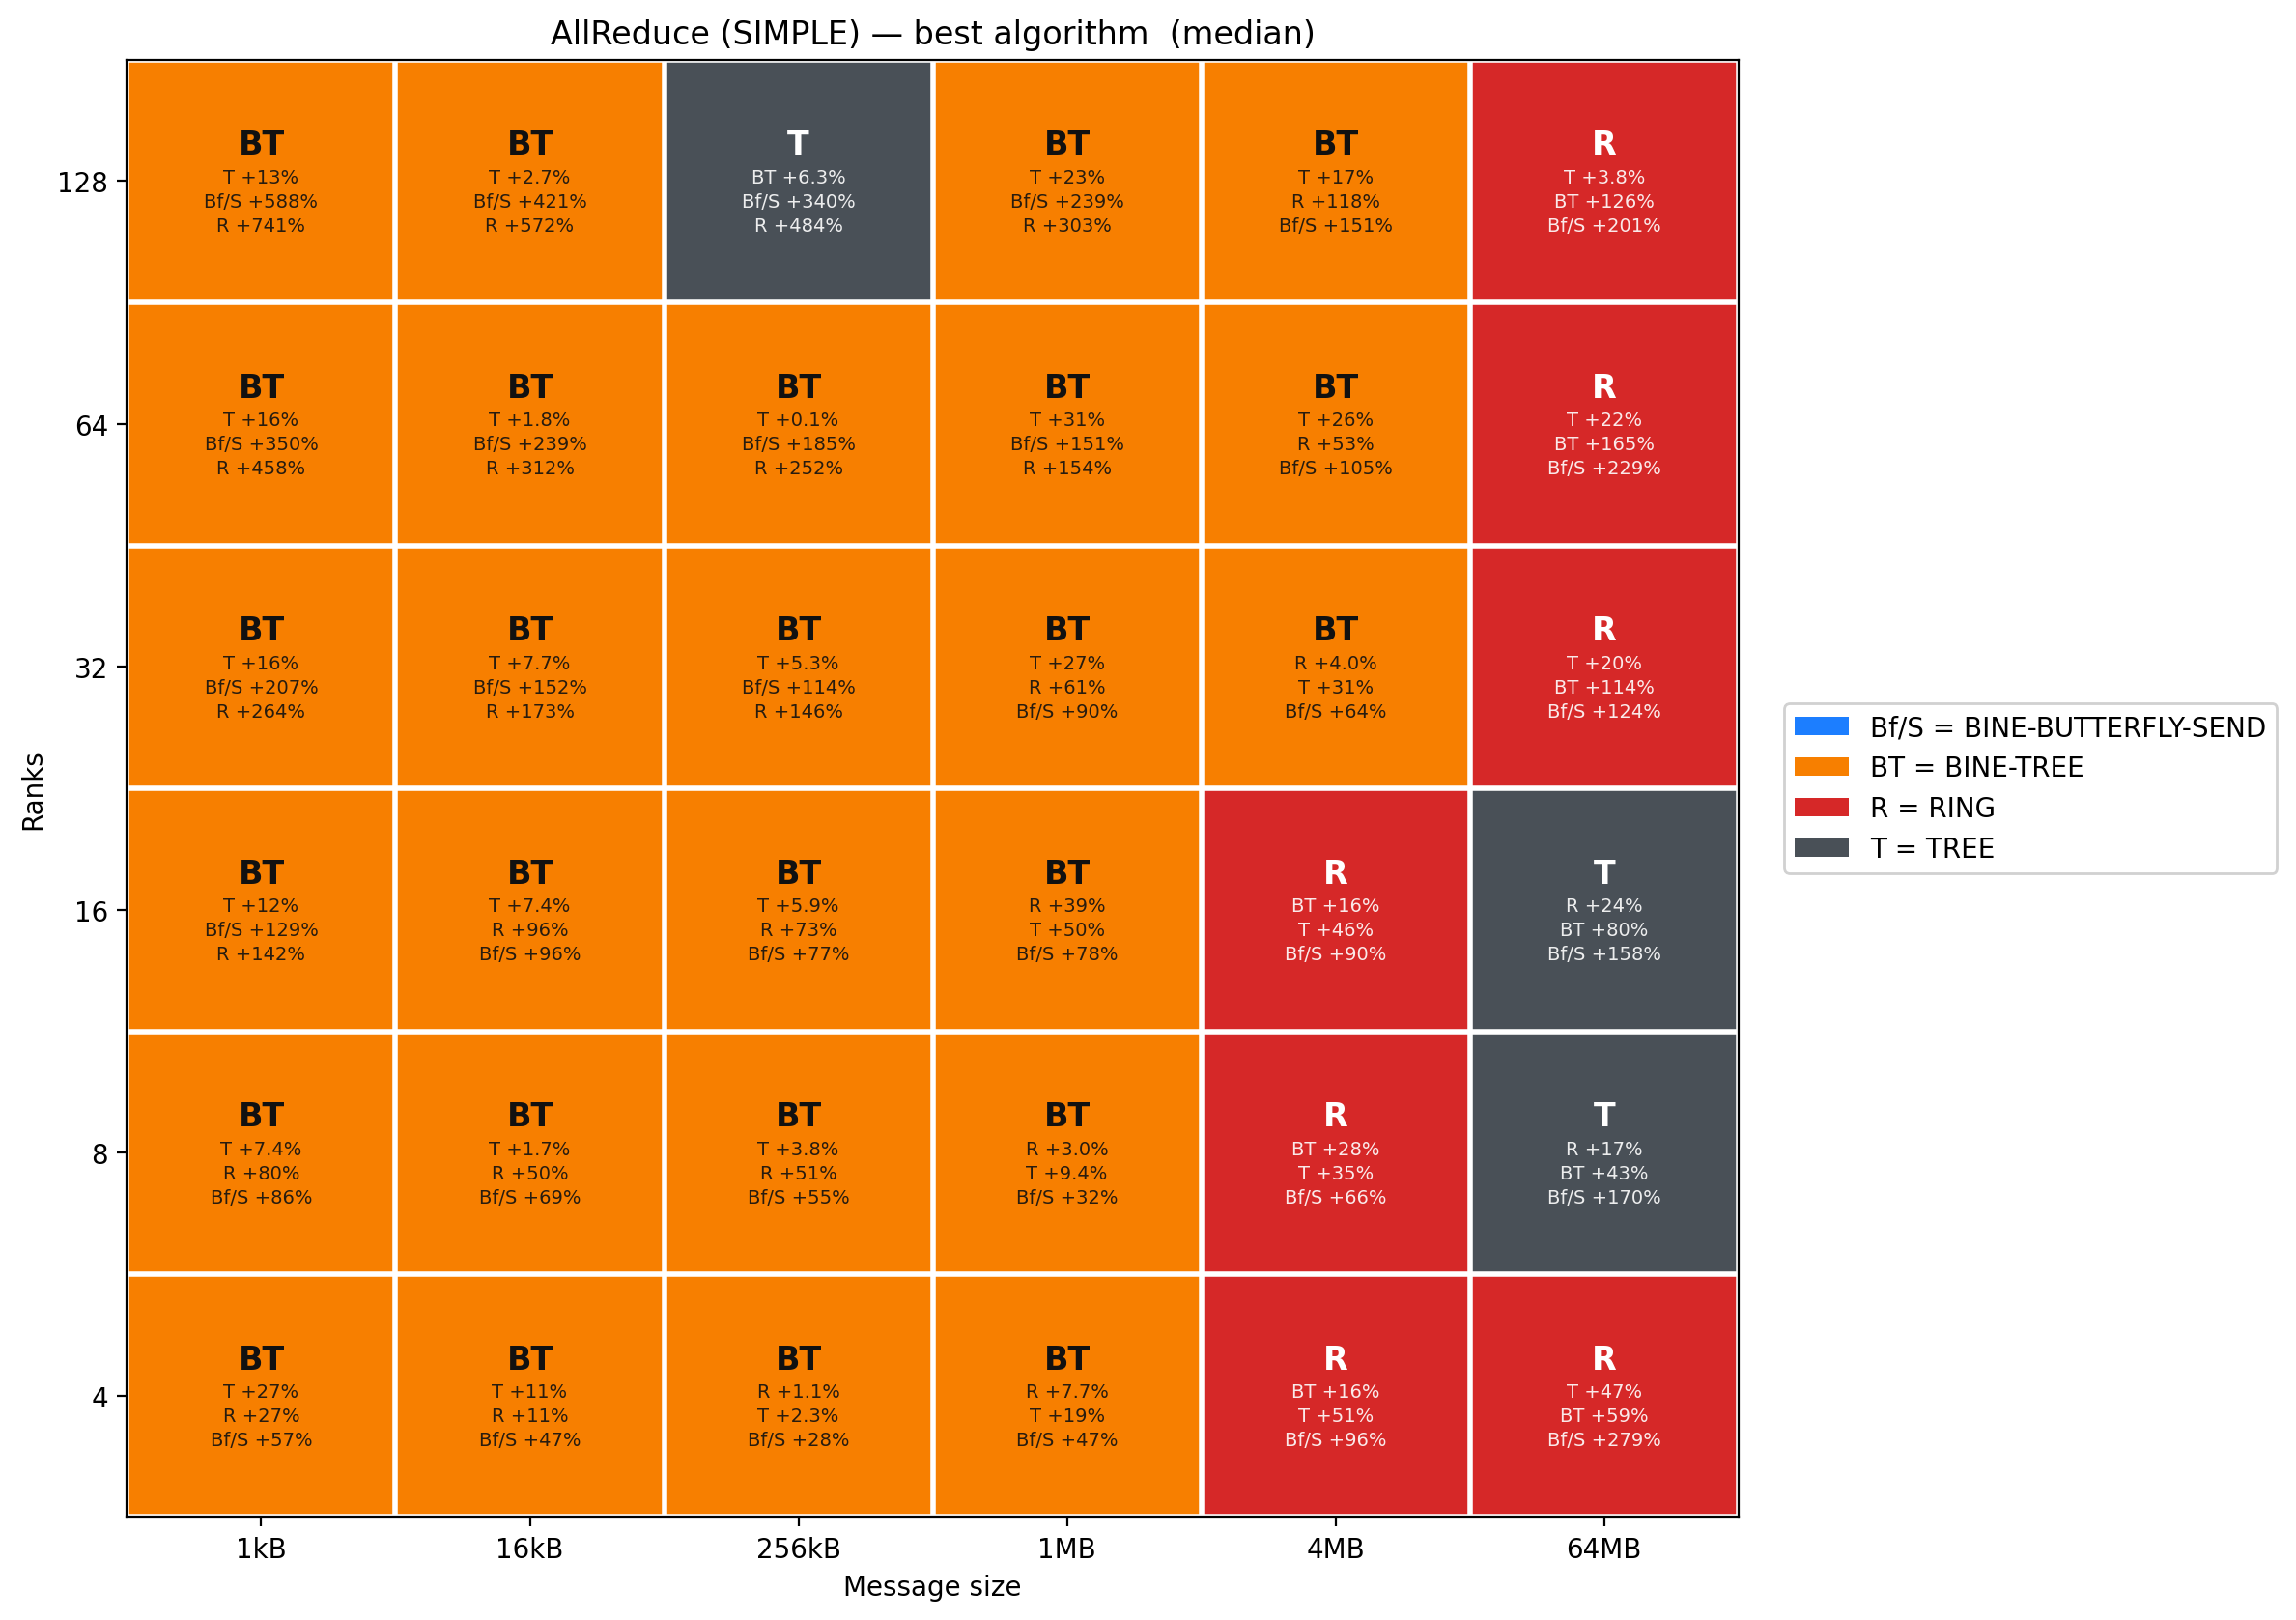
\includegraphics[width=0.66\linewidth]{AllReduce_SIMPLE_best_algo_heatmap.png}
  \caption{Fastest algorithm for each vector size and number of ranks with the \texttt{SIMPLE} protocol (median latency). Each cell lists the other algorithms with the percentage by which they are slower. BT: \bine{} tree, Bf/S: \bine{} butterfly (send), T: \nccl{} tree, R: \nccl{} ring.}
  \label{fig:tar-heatmap-simple}
\end{figure}
\paragraph{Simple protocol.}
With \texttt{SIMPLE}, the \bine{} tree is the fastest of the four algorithms in $26$ of the $36$ points (\cref{fig:tar-heatmap-simple}): all the points up to 1\,MB but one (256\,kB on $128$ ranks, where the \nccl{} tree is $6\,\%$ faster), and 4\,MB from $32$ ranks on. The ring and the \nccl{} tree are the fastest only at $4$ and 64\,MB.
Up to 1\,MB the \bine{} tree and the \nccl{} tree move the data the same way, a pipelined tree with the whole slice on every edge, even though the two trees differ in shape: the \nccl{} tree is a double binary tree, while the \bine{} tree allreduce of this chapter is a single binomial tree whose root changes with the channel, with exactly $\min(p,\mathit{nchannels})$ distinct roots across the channels (\cref{sec:tar-schedule}).
The \bine{} tree is faster in almost all the points: $29$ out of $36$ points are faster than the \nccl{} tree in the median.
The gain is consistent across scales: on average $15\,\%$ for 1\,kB, $5\,\%$ for 16\,kB and $2\,\%$ for 256\,kB, and it becomes sizeable for 1\,MB and 4\,MB ($26\,\%$ and $22\,\%$ on average, up to $1.5\times$ at 1\,MB on $16$ ranks).
The improvement over the ring is larger still for small vectors, because the latency of the ring is linear in $p$: for 1\,kB the \bine{} tree is $1.8\times$ faster than the ring on $8$ ranks and $8.4\times$ faster on $128$ ranks.
At 4\,MB the \bine{} tree is the fastest algorithm from $32$ ranks on, and the ring remains ahead on $4$ to $16$ ranks, by $14$ to $22\,\%$.
\begin{figure}[!htbp]
  \centering
  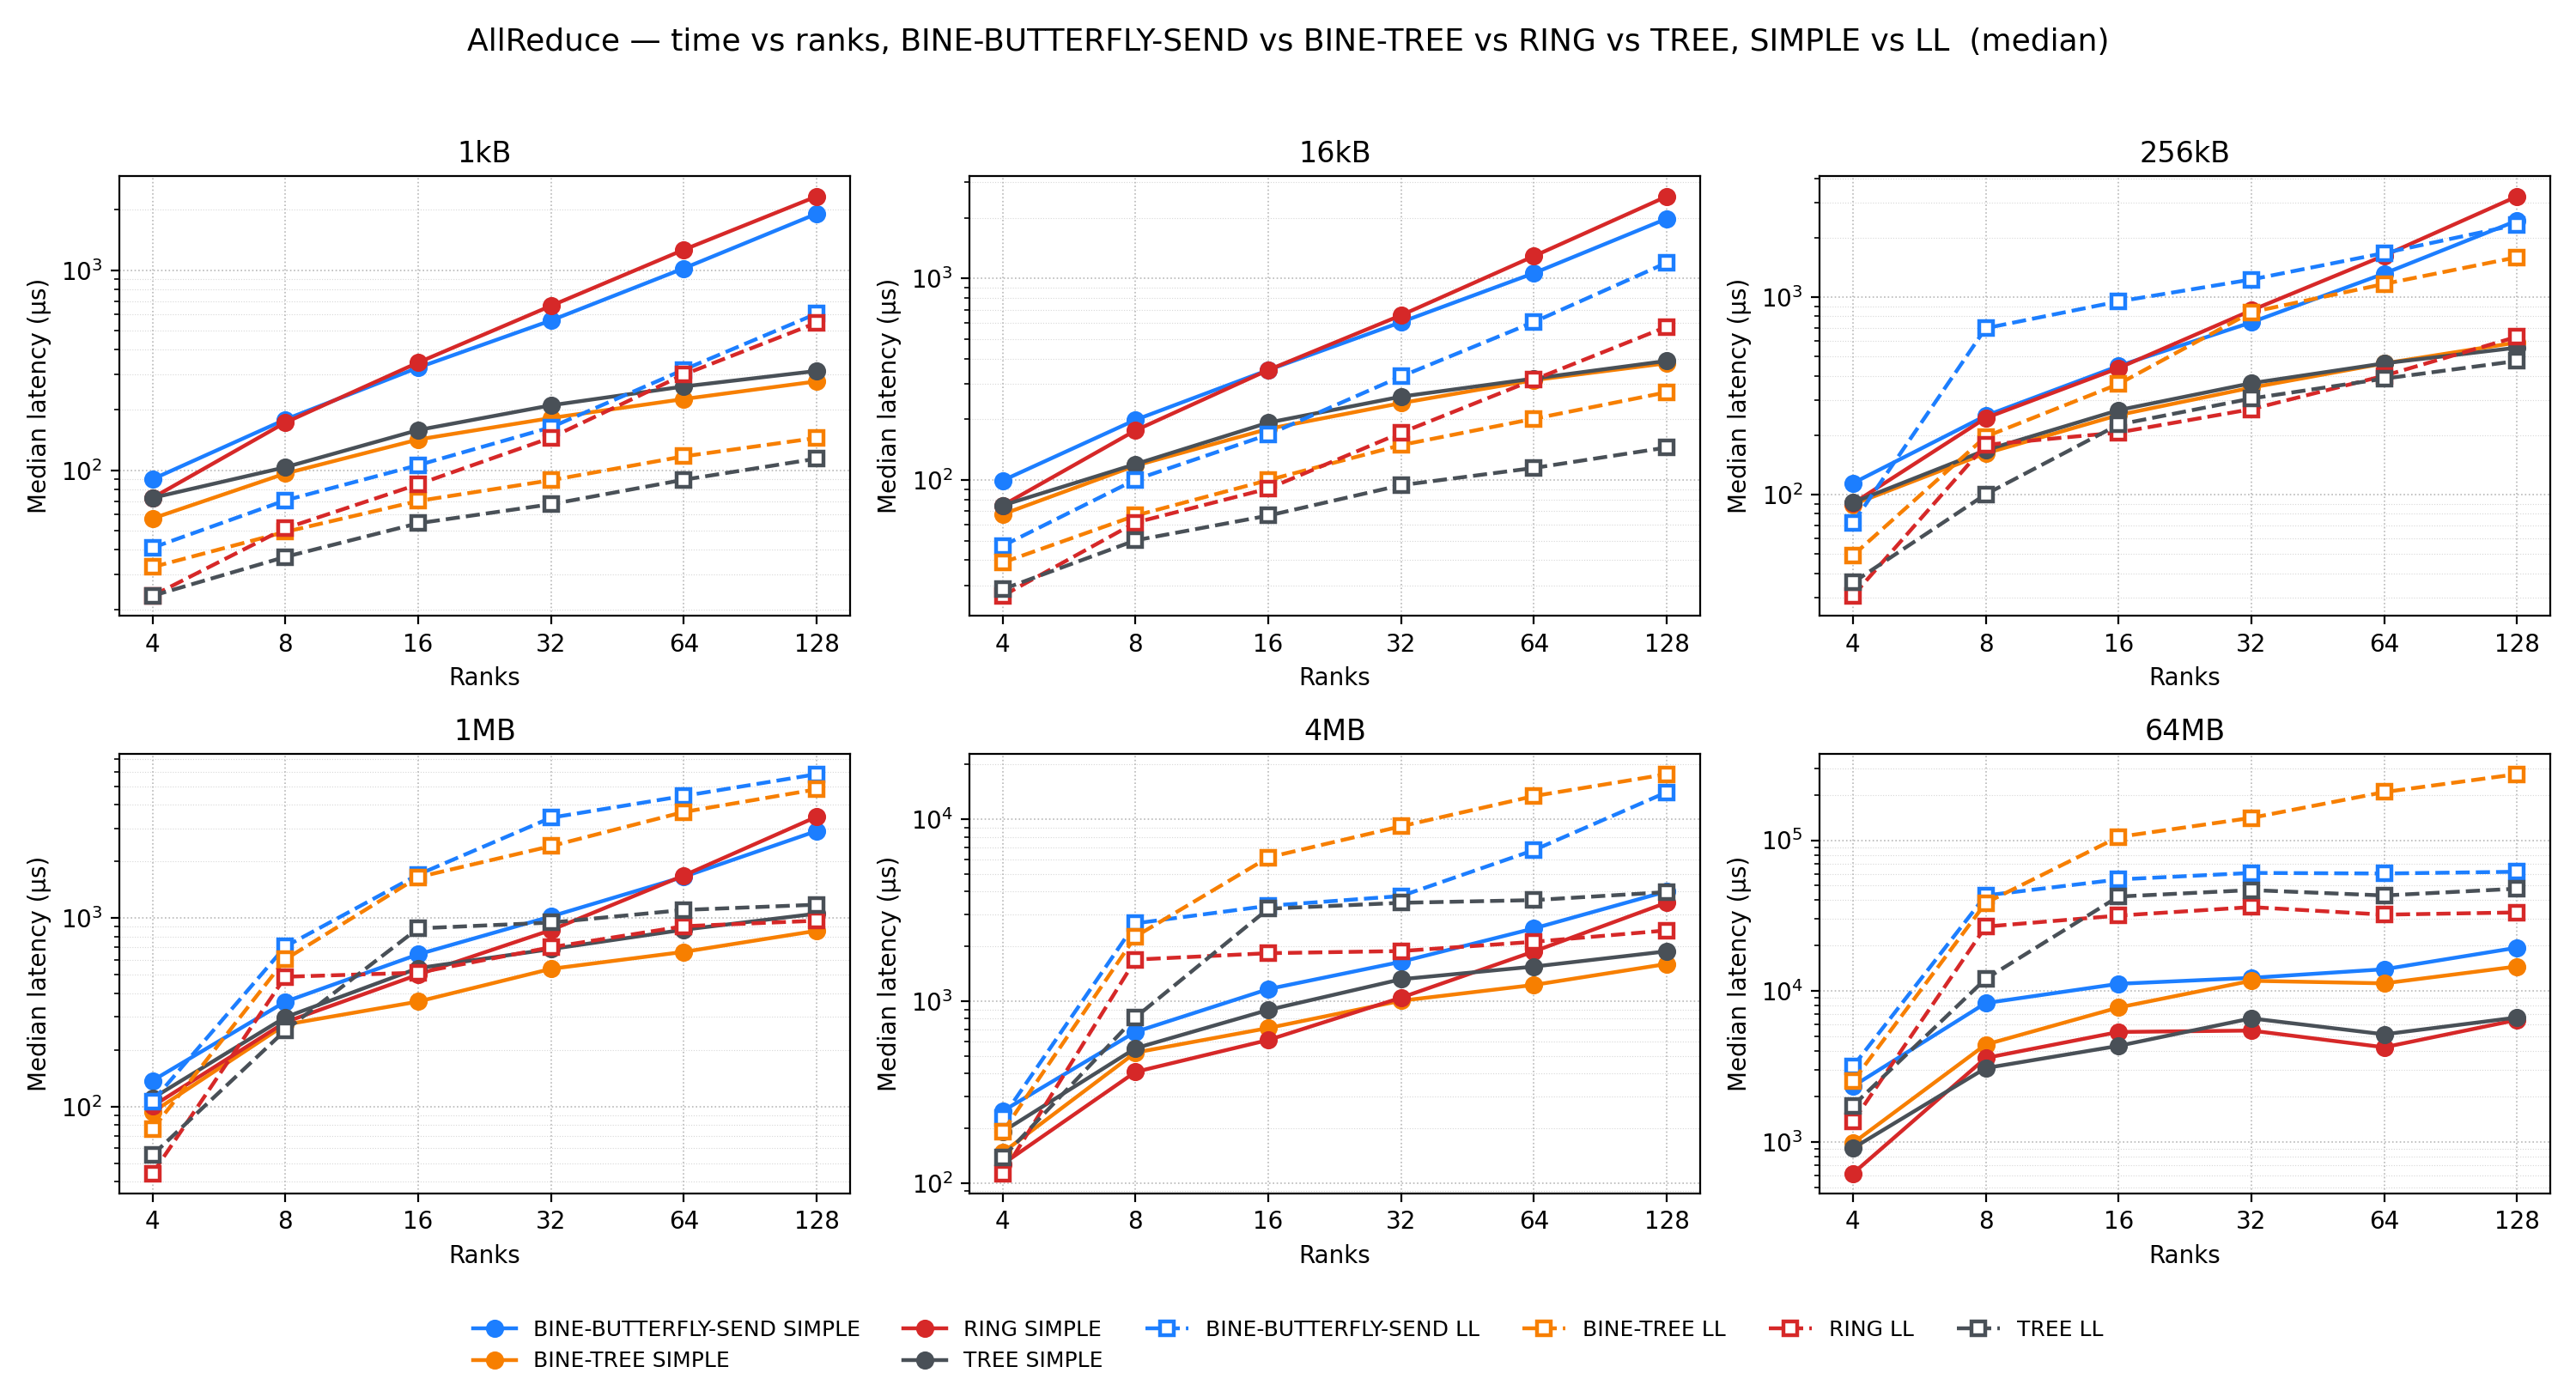
\includegraphics[width=0.95\linewidth]{AllReduce_SIMPLE+LL_vs_ranks_by_size.png}
  \caption{Median latency of the allreduce as a function of the number of ranks, for each vector size: \bine{} tree, \bine{} butterfly (send), \nccl{} tree and \nccl{} ring. Solid lines: \texttt{SIMPLE}. Dashed lines: \texttt{LL}. Both axes are logarithmic.}
  \label{fig:tar-scaling}
\end{figure}
\paragraph{Larger vectors and bandwidth.}
The \bine{} tree is not particularly bandwidth-efficient compared to the double binary tree of \nccl{}, and this becomes visible with the \texttt{SIMPLE} protocol for vectors larger than 4\,MB, and earlier with \texttt{LL}.
This is what the cost model of \cref{sec:tar-motivation} predicts: a binomial tree whose root has $\log_2p$ children sends each chunk $\log_2p$ times, so its bandwidth term grows with $p$, whereas the double binary tree of \nccl{} keeps it constant by splitting the data between two complementary trees, and the ring is bandwidth-optimal.
At 64\,MB the latency of the \bine{} tree with \texttt{SIMPLE} (\cref{fig:tar-scaling}) grows from 0.98\,ms on $4$ ranks to 4.4\,ms on $8$ and 14.6\,ms on $128$, in line with this explanation.
The \bine{} tree is therefore best suited to the range of sizes up to a few MB, which is the range in which the allreduce is latency-bound or in transition, and a natural extension is to give it the same two-tree structure as \nccl{} for large vectors.
\begin{figure}[!htbp]
  \centering
  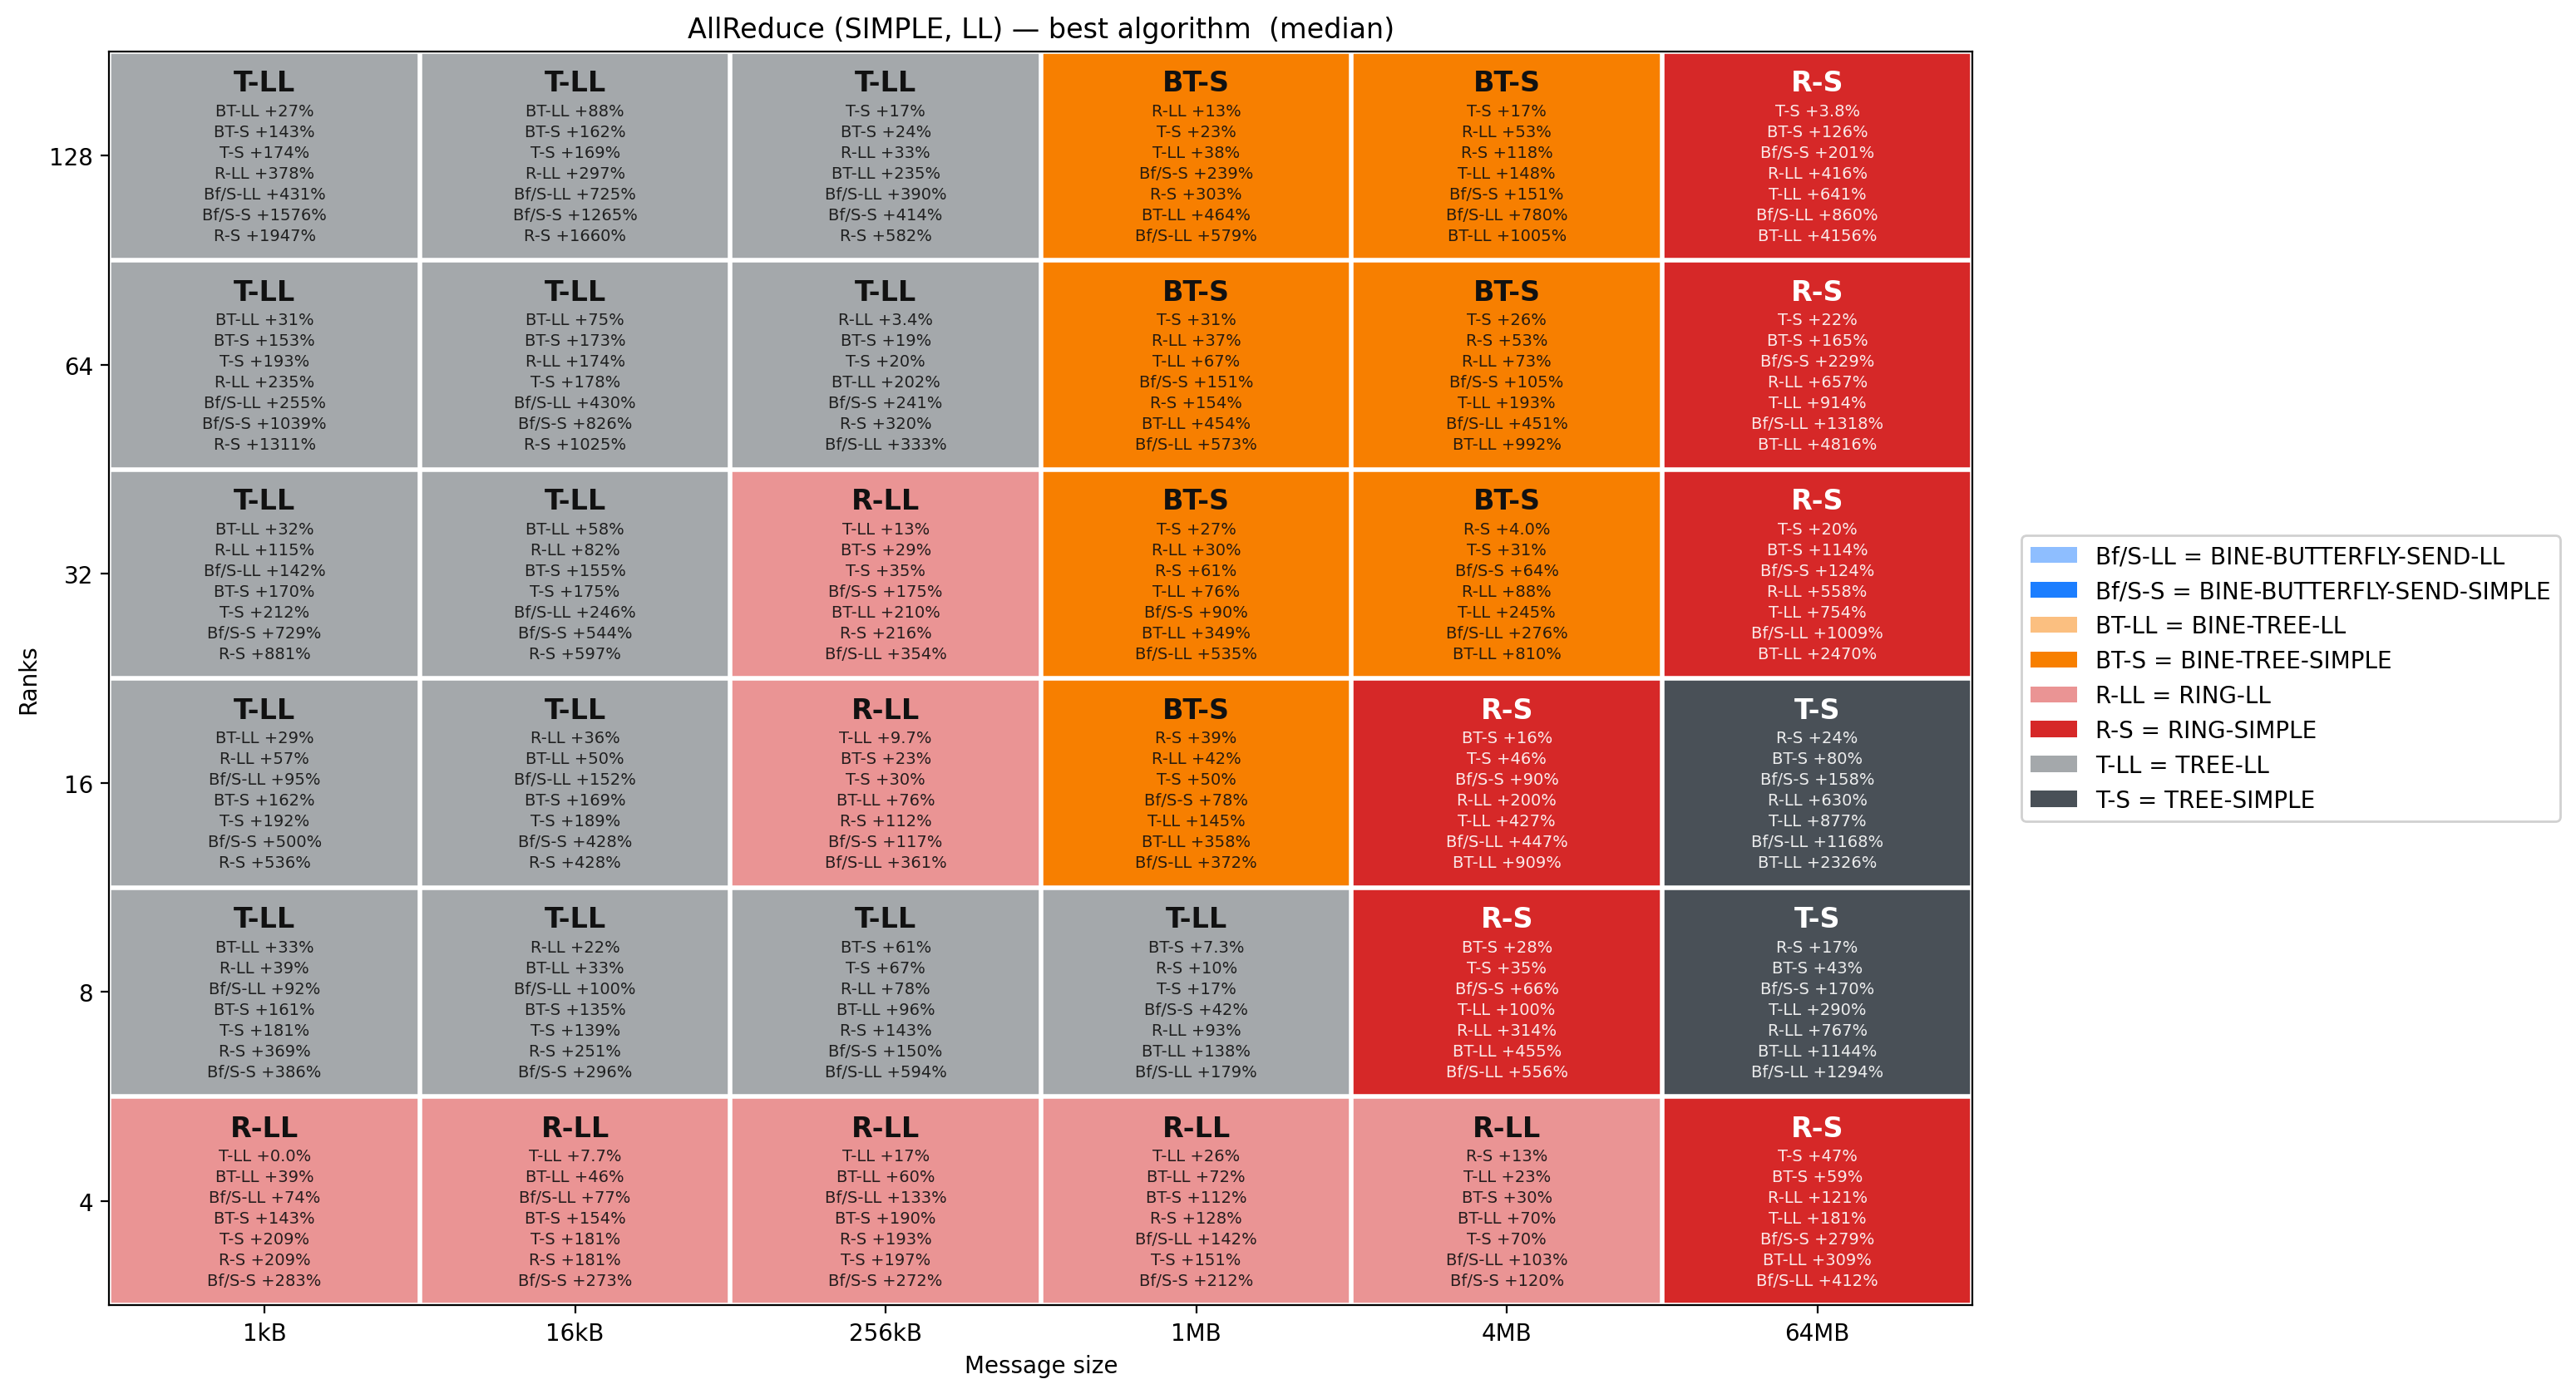
\includegraphics[width=0.95\linewidth]{AllReduce_SIMPLE+LL_best_algo_heatmap.png}
  \caption{Fastest algorithm for each vector size and number of ranks (median latency). Each cell lists the other combinations with the percentage by which they are slower. BT: \bine{} tree, Bf/S: \bine{} butterfly (send), T: \nccl{} tree, R: \nccl{} ring. The suffixes S and LL are the protocols.}
  \label{fig:tar-heatmap}
\end{figure}
\paragraph{LL protocol.}
With \texttt{LL}, which targets small messages, the \nccl{} tree and ring are the fastest algorithms, and the \bine{} tree remains within $27$ to $39\,\%$ of the best \nccl{} algorithm for 1\,kB (\cref{fig:tar-heatmap}).
For vectors above a few hundred kB the bandwidth term described above shows up earlier than with \texttt{SIMPLE}, since \texttt{LL} transfers a flag with every data word and has a lower effective bandwidth.
In this regime the \bine{} butterfly is faster than the \bine{} tree for 4\,MB and 64\,MB vectors from $16$ ranks on (\cref{fig:tar-scaling-bt}).
\begin{figure}[!htbp]
  \centering
  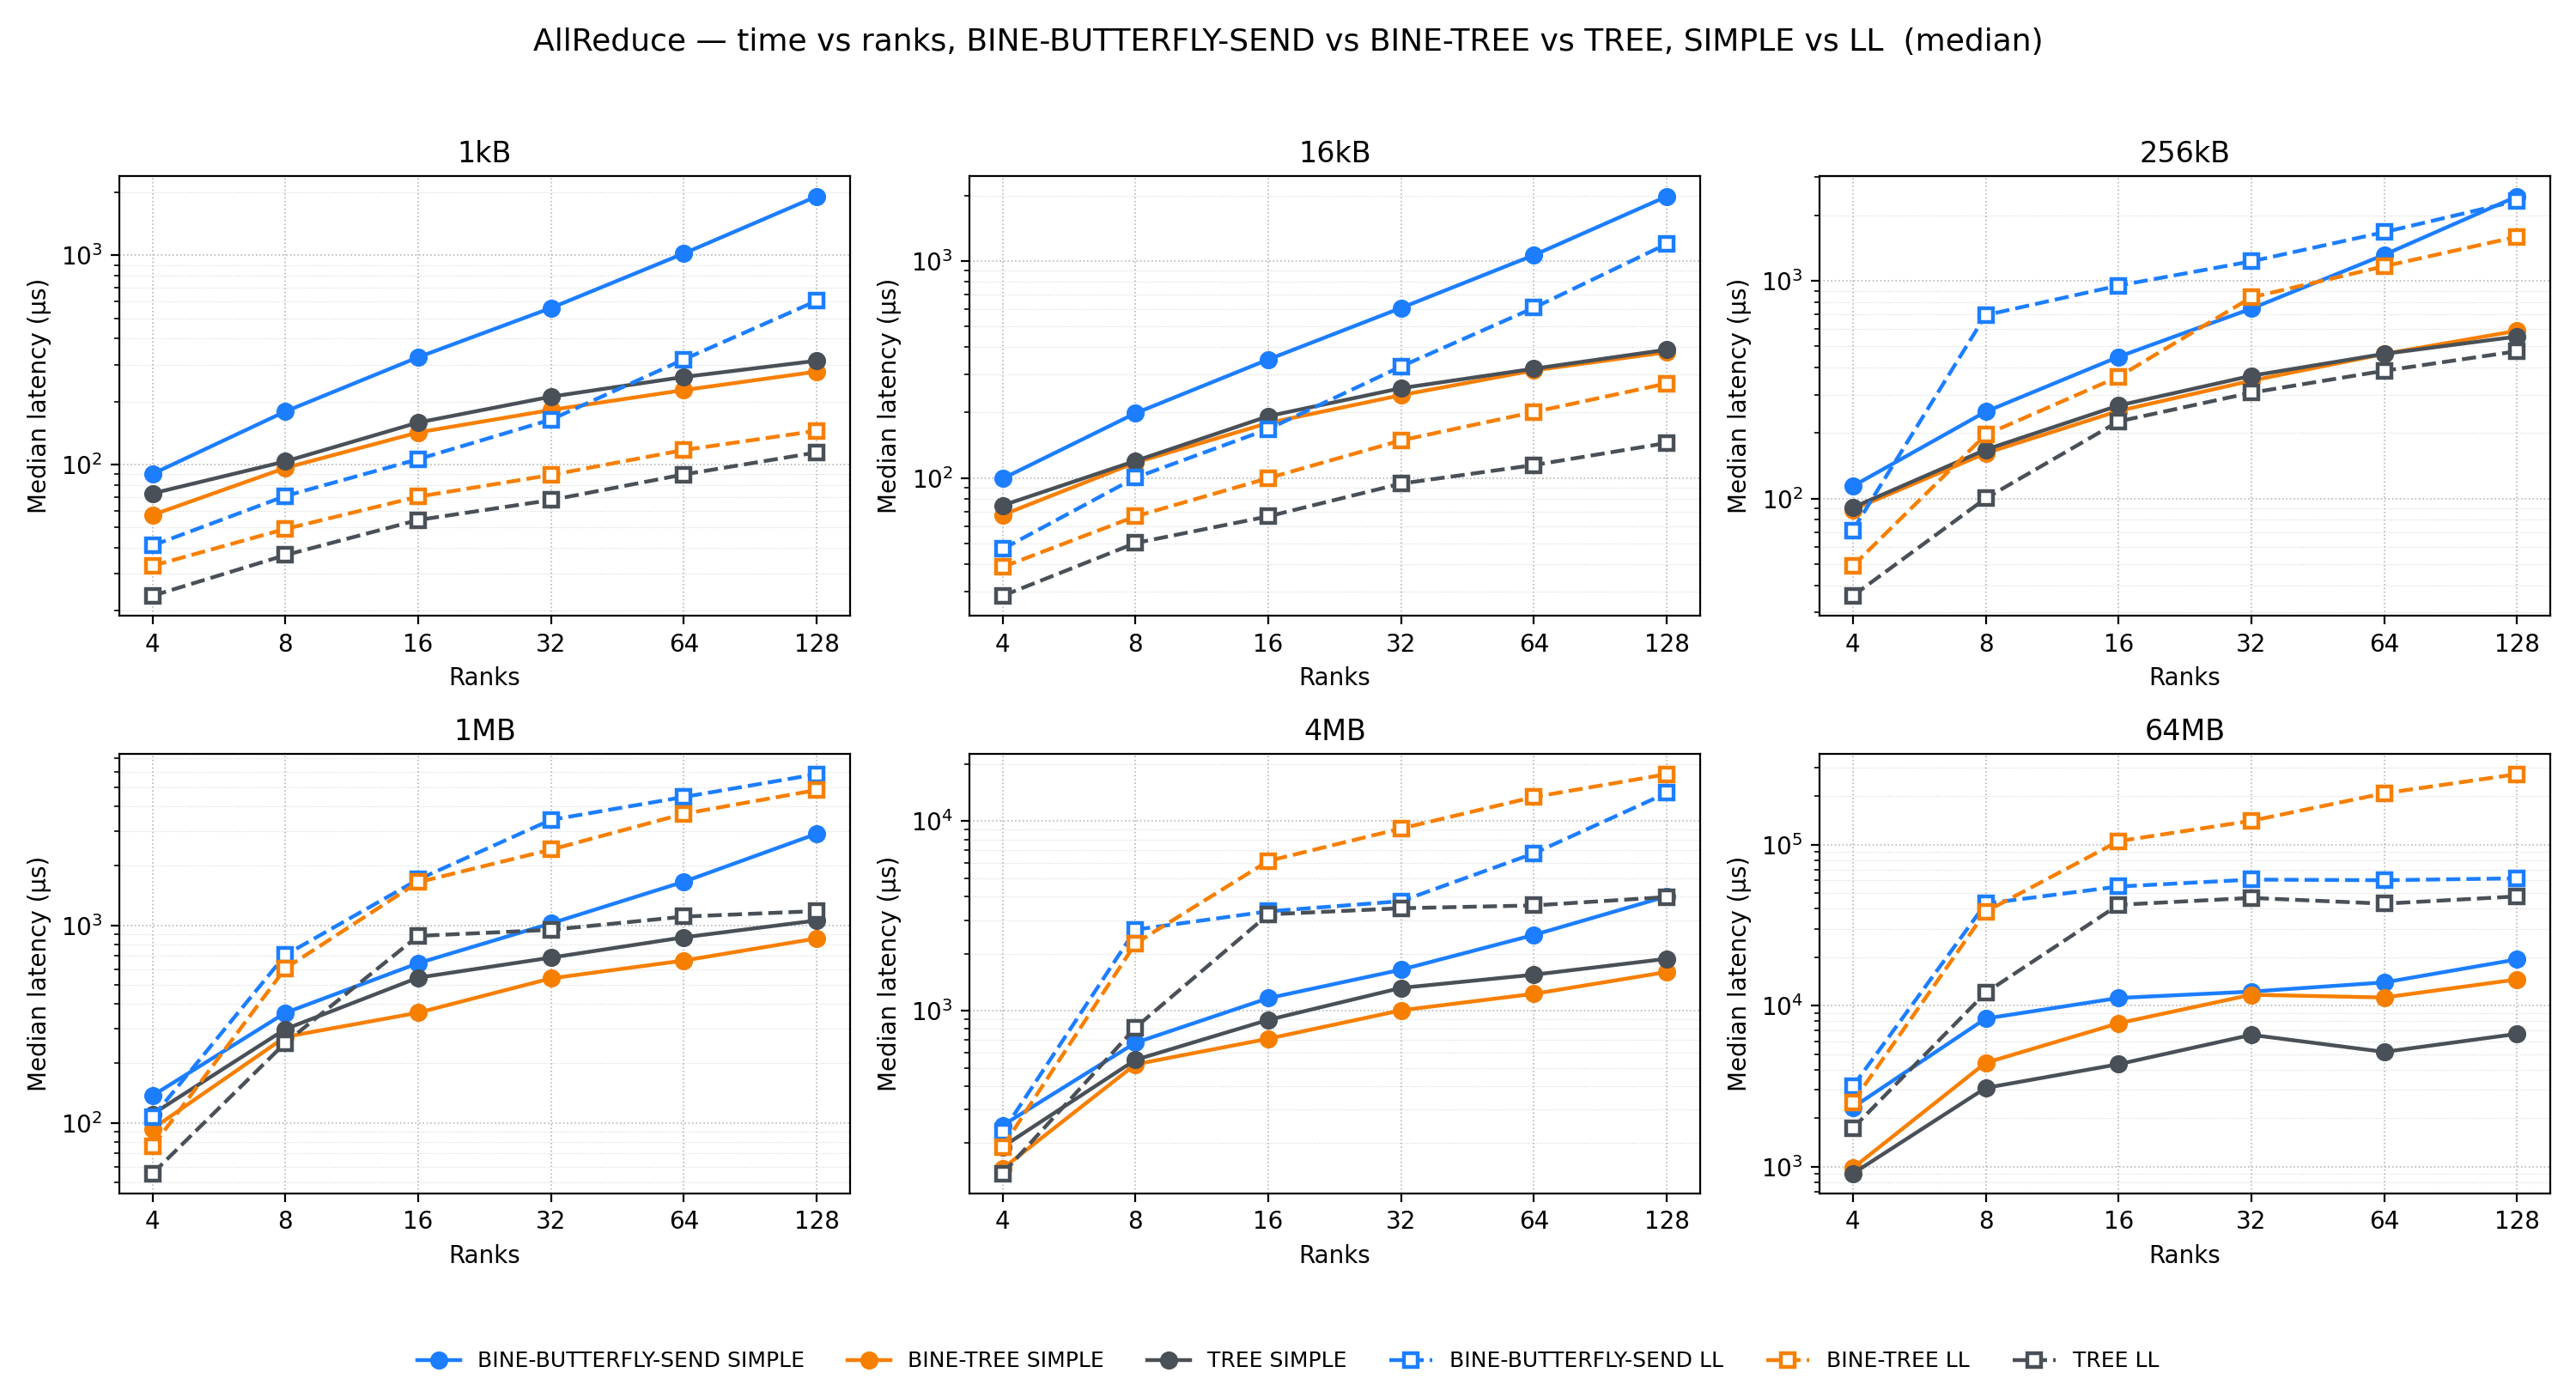
\includegraphics[width=0.95\linewidth]{AllReduce_SIMPLE+LL_vs_ranks_by_size_BINE+TREE.png}
  \caption{As \cref{fig:tar-scaling}, without the \nccl{} ring, to separate the \bine{} tree, the \nccl{} tree and the \bine{} butterfly.}
  \label{fig:tar-scaling-bt}
\end{figure}
\paragraph{Butterfly.}
The \bine{} butterfly allreduce is useful as a reference for what a different structure costs inside \nccl{}.
With \texttt{SIMPLE} it takes between $1.2\times$ and $6.1\times$ the time of the best \nccl{} algorithm, and for small vectors the gap grows with $p$ ($1.2\times$ on $4$ ranks and $6.1\times$ on $128$ ranks for 1\,kB).
This is consistent with the motivation of \cref{sec:tar-motivation}: the butterfly has to handle windows of different sizes at each step on top of the fixed partition of \nccl{}, which the \bine{} tree avoids.
For the largest vectors in \texttt{LL}, on the other hand, the butterfly improves over the \bine{} tree.
\paragraph{Summary.}
With the \texttt{SIMPLE} protocol, for vectors from 1\,kB to a few MB, the \bine{} tree allreduce is on par with or faster than the \nccl{} tree and, for medium sizes on many ranks, than the ring, keeping the partition of \nccl{} unchanged and without a schedule thread or a staging buffer.
For large vectors the bandwidth efficiency of the double binary tree and of the ring is higher, which defines the natural operating range of the \bine{} tree allreduce.

% Software developed for the thesis.
% Uses the macros of the preamble (\nccl, \bine, \pat) and the colors ch0, ch1, crosslink, localxfer.

\chapter{Software Developed}\label{ch:software}

The algorithms of the previous chapters were developed in two stages.
The schedules were first prototyped as plain MPI collectives, where every message is visible and can be timed, and only then moved inside \nccl{}, where they are executed by GPU kernels and can only be observed from outside.
Each stage has its own pair of tools (\cref{fig:sw-overview}):
\begin{itemize}
  \item \textbf{CollBench} and \textbf{Collalgo} cover the MPI stage. Collalgo implements the \bine{} collectives over MPI point-to-point calls, and CollBench records the timing of each of those calls, so that a schedule can be checked and inspected message by message.
  \item \textbf{fastest} and \textbf{unitccl} cover the \nccl{} stage. fastest is a small test framework for C code driven from Python, and unitccl uses it to unit-test the schedule generators of the \nccl{} fork and to run the scaling experiments, either with its own benchmark or with NVIDIA's \texttt{nccl-tests}.
\end{itemize}
All four are available on GitHub under the author's account (\texttt{DanieleSavino}). The \nccl{} fork that contains the algorithms is a separate repository and is the subject of \cref{ch:tree,ch:butterfly,ch:pat,ch:treeallreduce}.

\begin{figure}[htbp]
  \centering
  \begin{tikzpicture}[x=1cm, y=1cm,
      repo/.style={draw, rounded corners=2pt, thick, minimum width=2.9cm, minimum height=0.9cm,
                   align=center, font=\small, fill=white},
      ext/.style={draw, dashed, rounded corners=2pt, minimum width=2.9cm, minimum height=0.9cm,
                  align=center, font=\small, text=black!70},
      dep/.style={-{Stealth[length=2mm]}, thick},
      use/.style={-{Stealth[length=2mm]}, thick, dashed, black!55}]
    % MPI stage
    \node[repo, draw=ch0] (cb) at (0,0) {CollBench\\[-1pt]\scriptsize C99, MPI};
    \node[repo, draw=ch0] (ca) at (0,2) {Collalgo\\[-1pt]\scriptsize C11, MPI, CUDA};
    \node[ext] (viz) at (0,-1.9) {JSON traces\\[-1pt]\scriptsize Python plots};
    \draw[dep] (ca) -- node[right, font=\scriptsize] {submodule} (cb);
    \draw[use] (cb) -- node[right, font=\scriptsize] {export} (viz);
    % NCCL stage
    \node[repo, draw=ch1] (fa) at (4.6,0) {fastest\\[-1pt]\scriptsize C11, pybind11, Python};
    \node[repo, draw=ch1] (uc) at (4.6,2) {unitccl\\[-1pt]\scriptsize C/CUDA, Python CLI};
    \node[ext] (nccl) at (8.3,2.9) {\nccl{} fork};
    \node[ext] (nt) at (8.3,1.1) {\texttt{nccl-tests}};
    \draw[dep] (uc) -- node[left, font=\scriptsize] {submodule} (fa);
    \draw[dep] (uc.east) -- ++(0.35,0) |- (nccl.west);
    \draw[use] (uc.east) -- ++(0.35,0) |- (nt.west);
    % stage labels
    \begin{scope}[on background layer]
      \node[fit=(cb)(ca)(viz), fill=ch0!8, rounded corners=4pt, inner sep=7pt,
            label={[font=\small]above:MPI prototyping}] {};
      \node[fit=(fa)(uc)(nccl)(nt)(viz.south -| fa), fill=ch1!8, rounded corners=4pt, inner sep=7pt,
            label={[font=\small]above:\nccl{} testing and benchmarking}] {};
    \end{scope}
  \end{tikzpicture}
  \caption{The four repositories. Solid arrows: build-time dependencies (git submodules and static linking). Dashed arrows: tools that are driven or whose output is consumed.}
  \label{fig:sw-overview}
\end{figure}

% ---------------------------------------------------------------------------
\section{CollBench}\label{sec:sw-collbench}

CollBench is a C99 library that profiles the point-to-point operations of a collective written over MPI.
Timing a collective as a whole says how long it took, but not \emph{why}: whether a step waits for a late sender, whether one link is slower than the others, or whether the schedule does what the algorithm prescribes.
CollBench answers these questions by recording every send and receive issued by every rank, with the step of the algorithm it belongs to, and by collecting the records of all the ranks into a single trace.

\paragraph{Operation records.}
Each operation is described by a \texttt{CB\_OperationData\_t}: the rank that posts it, the peer, the type of operation (send, receive or one of the collectives), the step index of the algorithm (\texttt{algo\_idx}), and three timestamps taken with \texttt{CLOCK\_MONOTONIC}: when the operation is posted, when the rank starts waiting on it, and when it completes.
For a blocking operation the last two coincide. For a non-blocking one their difference separates the time spent issuing the operation from the time spent waiting for it, which shows how much computation or other communication overlaps with it.
The records of a rank are appended to a growable list (\texttt{CB\_DistList\_t}).

\paragraph{Instrumentation macros.}
A collective is instrumented by replacing its MPI calls with the CollBench macros and enclosing its body in a profiling scope:
\begin{lstlisting}[language=C, numbers=none]
CB_COLL_START();
for (...) {                                     /* one iteration per step */
  if (sender) CB_LSEND(rank, step, buf, n, dt, peer, tag, comm);
  else        CB_LRECV(rank, step, buf, n, dt, peer, tag, comm);
}
CB_COLL_END(comm, rank, root, "out/tree/bine_bcast.json");
\end{lstlisting}
\texttt{CB\_LSEND} and \texttt{CB\_LRECV} post the operation, wait for it and record it. The non-blocking variants \texttt{CB\_ILSEND} and \texttt{CB\_ILRECV} record the posting time and leave the request to \texttt{CB\_LWAIT} or \texttt{CB\_LWAITALL}.
\texttt{CB\_COLL\_END} gathers the lists of all the ranks onto the root with an \texttt{MPI\_Gatherv} (the records travel as an MPI derived datatype registered by \texttt{CB\_init}) and the root writes them as JSON.
All the macros are compiled only when \texttt{CB\_PROFILE} is defined. Otherwise they expand to the bare MPI calls, so the same source builds both the profiled and the production version of a collective with no overhead in the latter.
Errors are propagated as \texttt{CB\_Error\_t} codes through \texttt{goto}-based cleanup labels, which the scope macros define.

\paragraph{Visualization.}
Two Python scripts turn a trace into a picture.
\texttt{tree.py} detects whether the collective flows away from the root (broadcast, scatter) or towards it (reduce, gather), rebuilds the tree from the send records and draws it by step, annotating each edge with the duration of the transfer (\cref{fig:sw-cb-tree}).
\texttt{butterfly.py} does the same for collectives without a root, in which every rank exchanges with a partner at every step.
Its \emph{candle} view (\cref{fig:sw-cb-candle}) draws each rank as a horizontal lane and each exchange as a vertical connector between the two lanes, one column per pair, grouped by step, so that the pairing of a step and the distance between partners are read at a glance. The other views draw the same exchanges as a rank-by-step grid, as a ladder, or as the $p$ broadcast trees that a butterfly allgather implicitly contains, one per source block.
These drawings are how the schedules of \cref{ch:tree,ch:butterfly} were checked visually against the figures of the algorithms before they were moved to \nccl{}.

\begin{figure}[!tbp]
  \centering
  \captionsetup[subfigure]{skip=2pt}
  \begin{subfigure}{\linewidth}
    \centering
    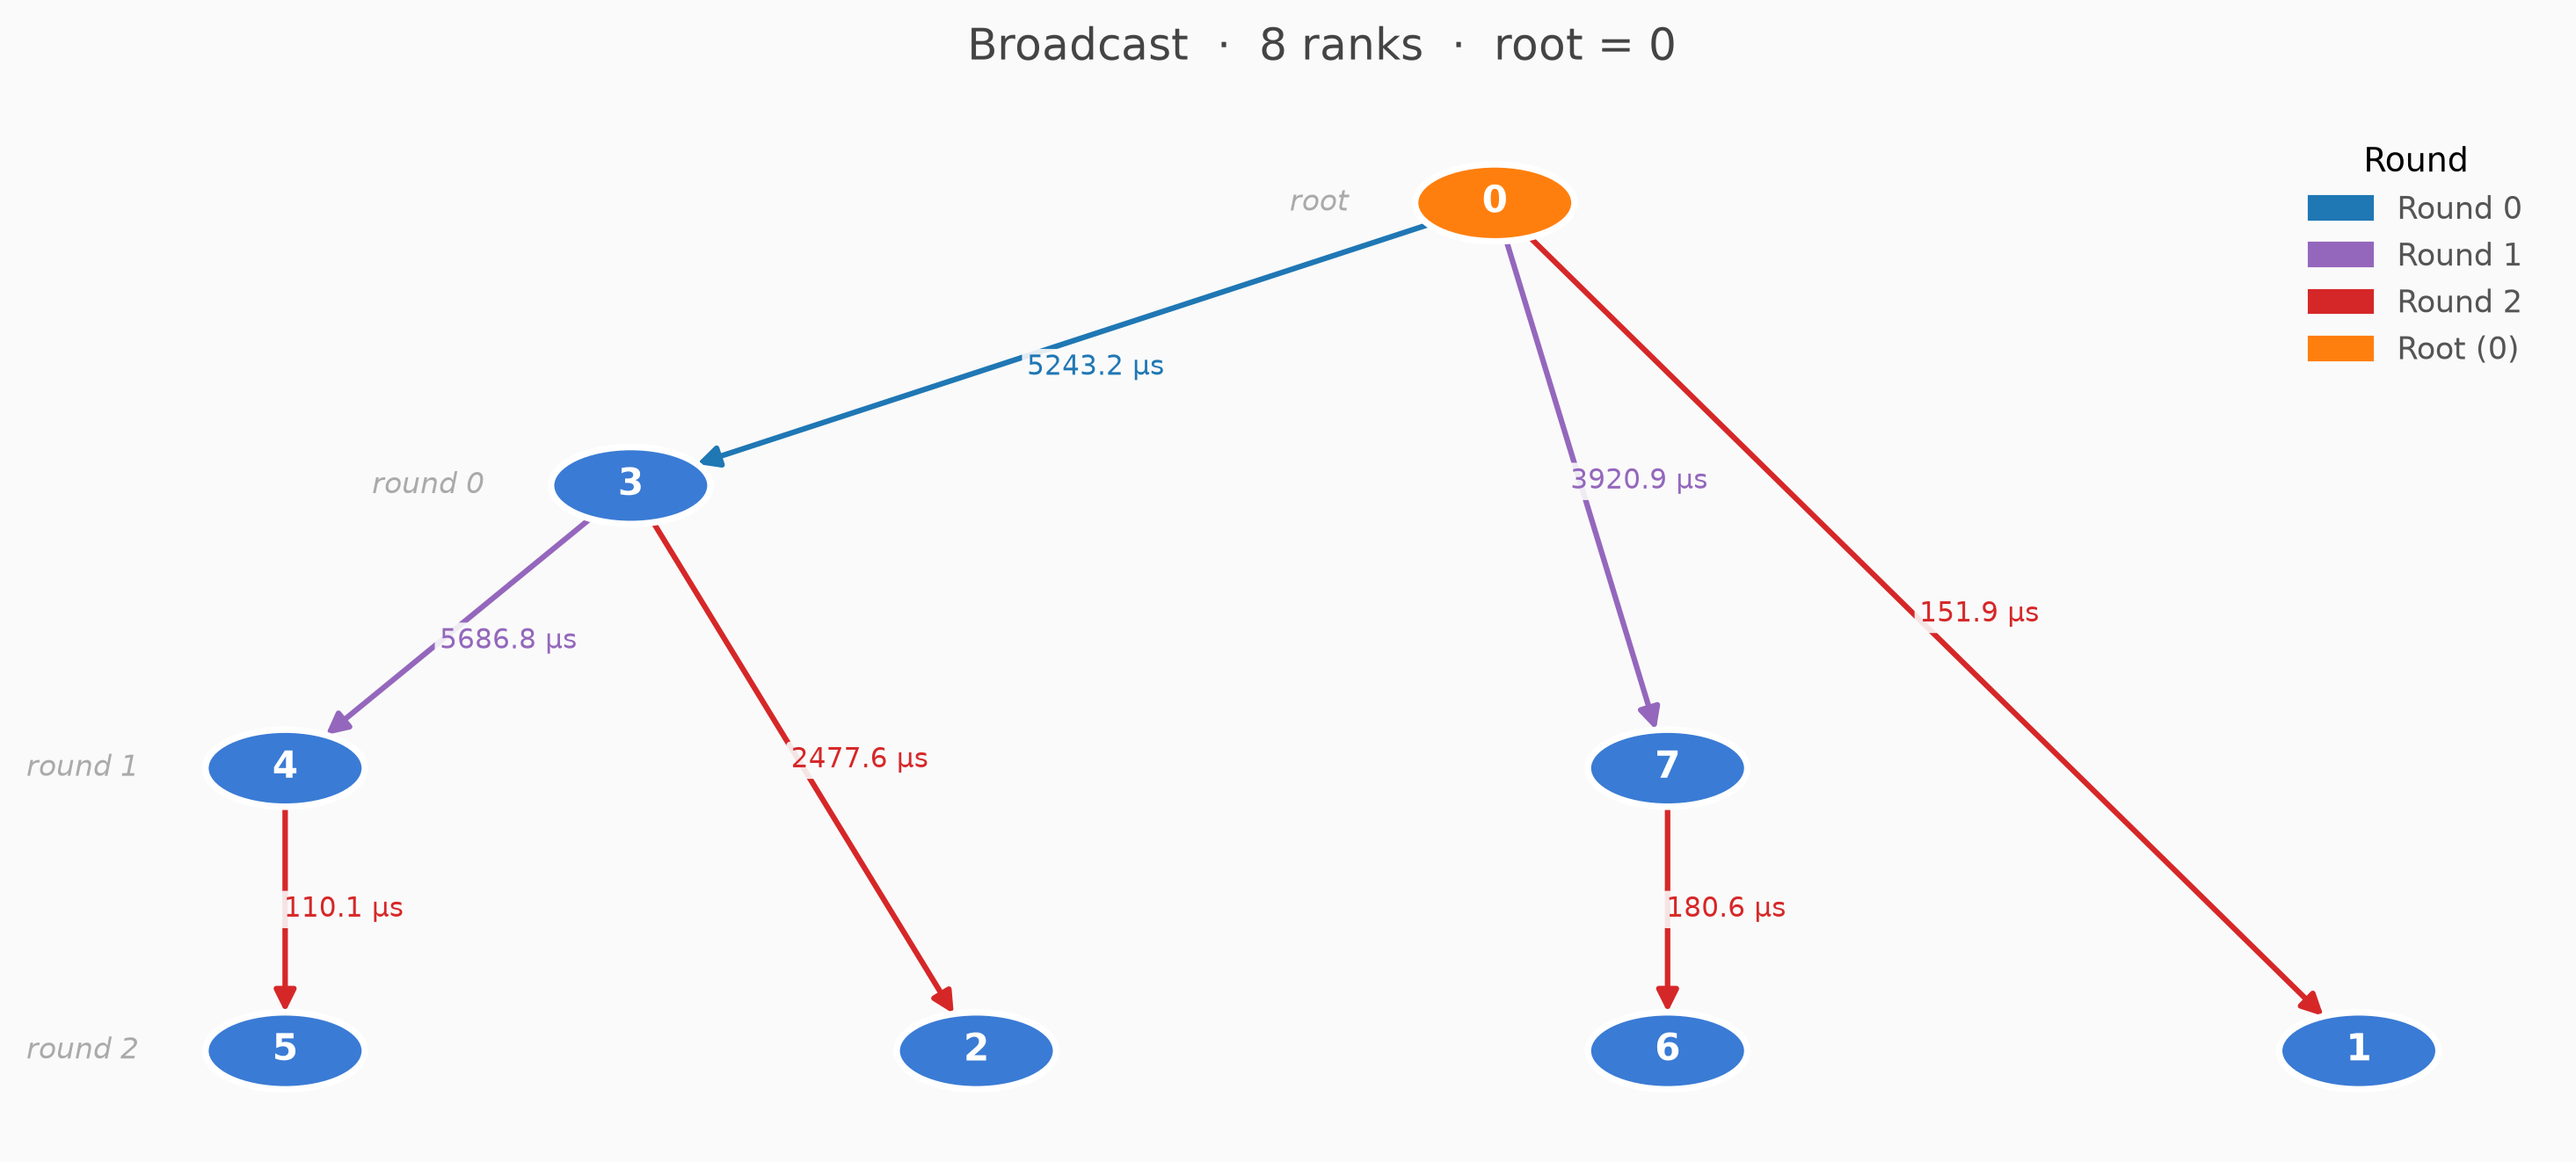
\includegraphics[width=0.8\linewidth]{collbench_bcast_tree.png}
    \caption{Distance-halving \bine{} broadcast, drawn by \texttt{tree.py}. Each edge is a send, labelled with the time from posting it to its completion, which includes the time the receiver takes to reach the matching receive.}
    \label{fig:sw-cb-tree}
  \end{subfigure}

  \medskip
  \begin{subfigure}{\linewidth}
    \centering
    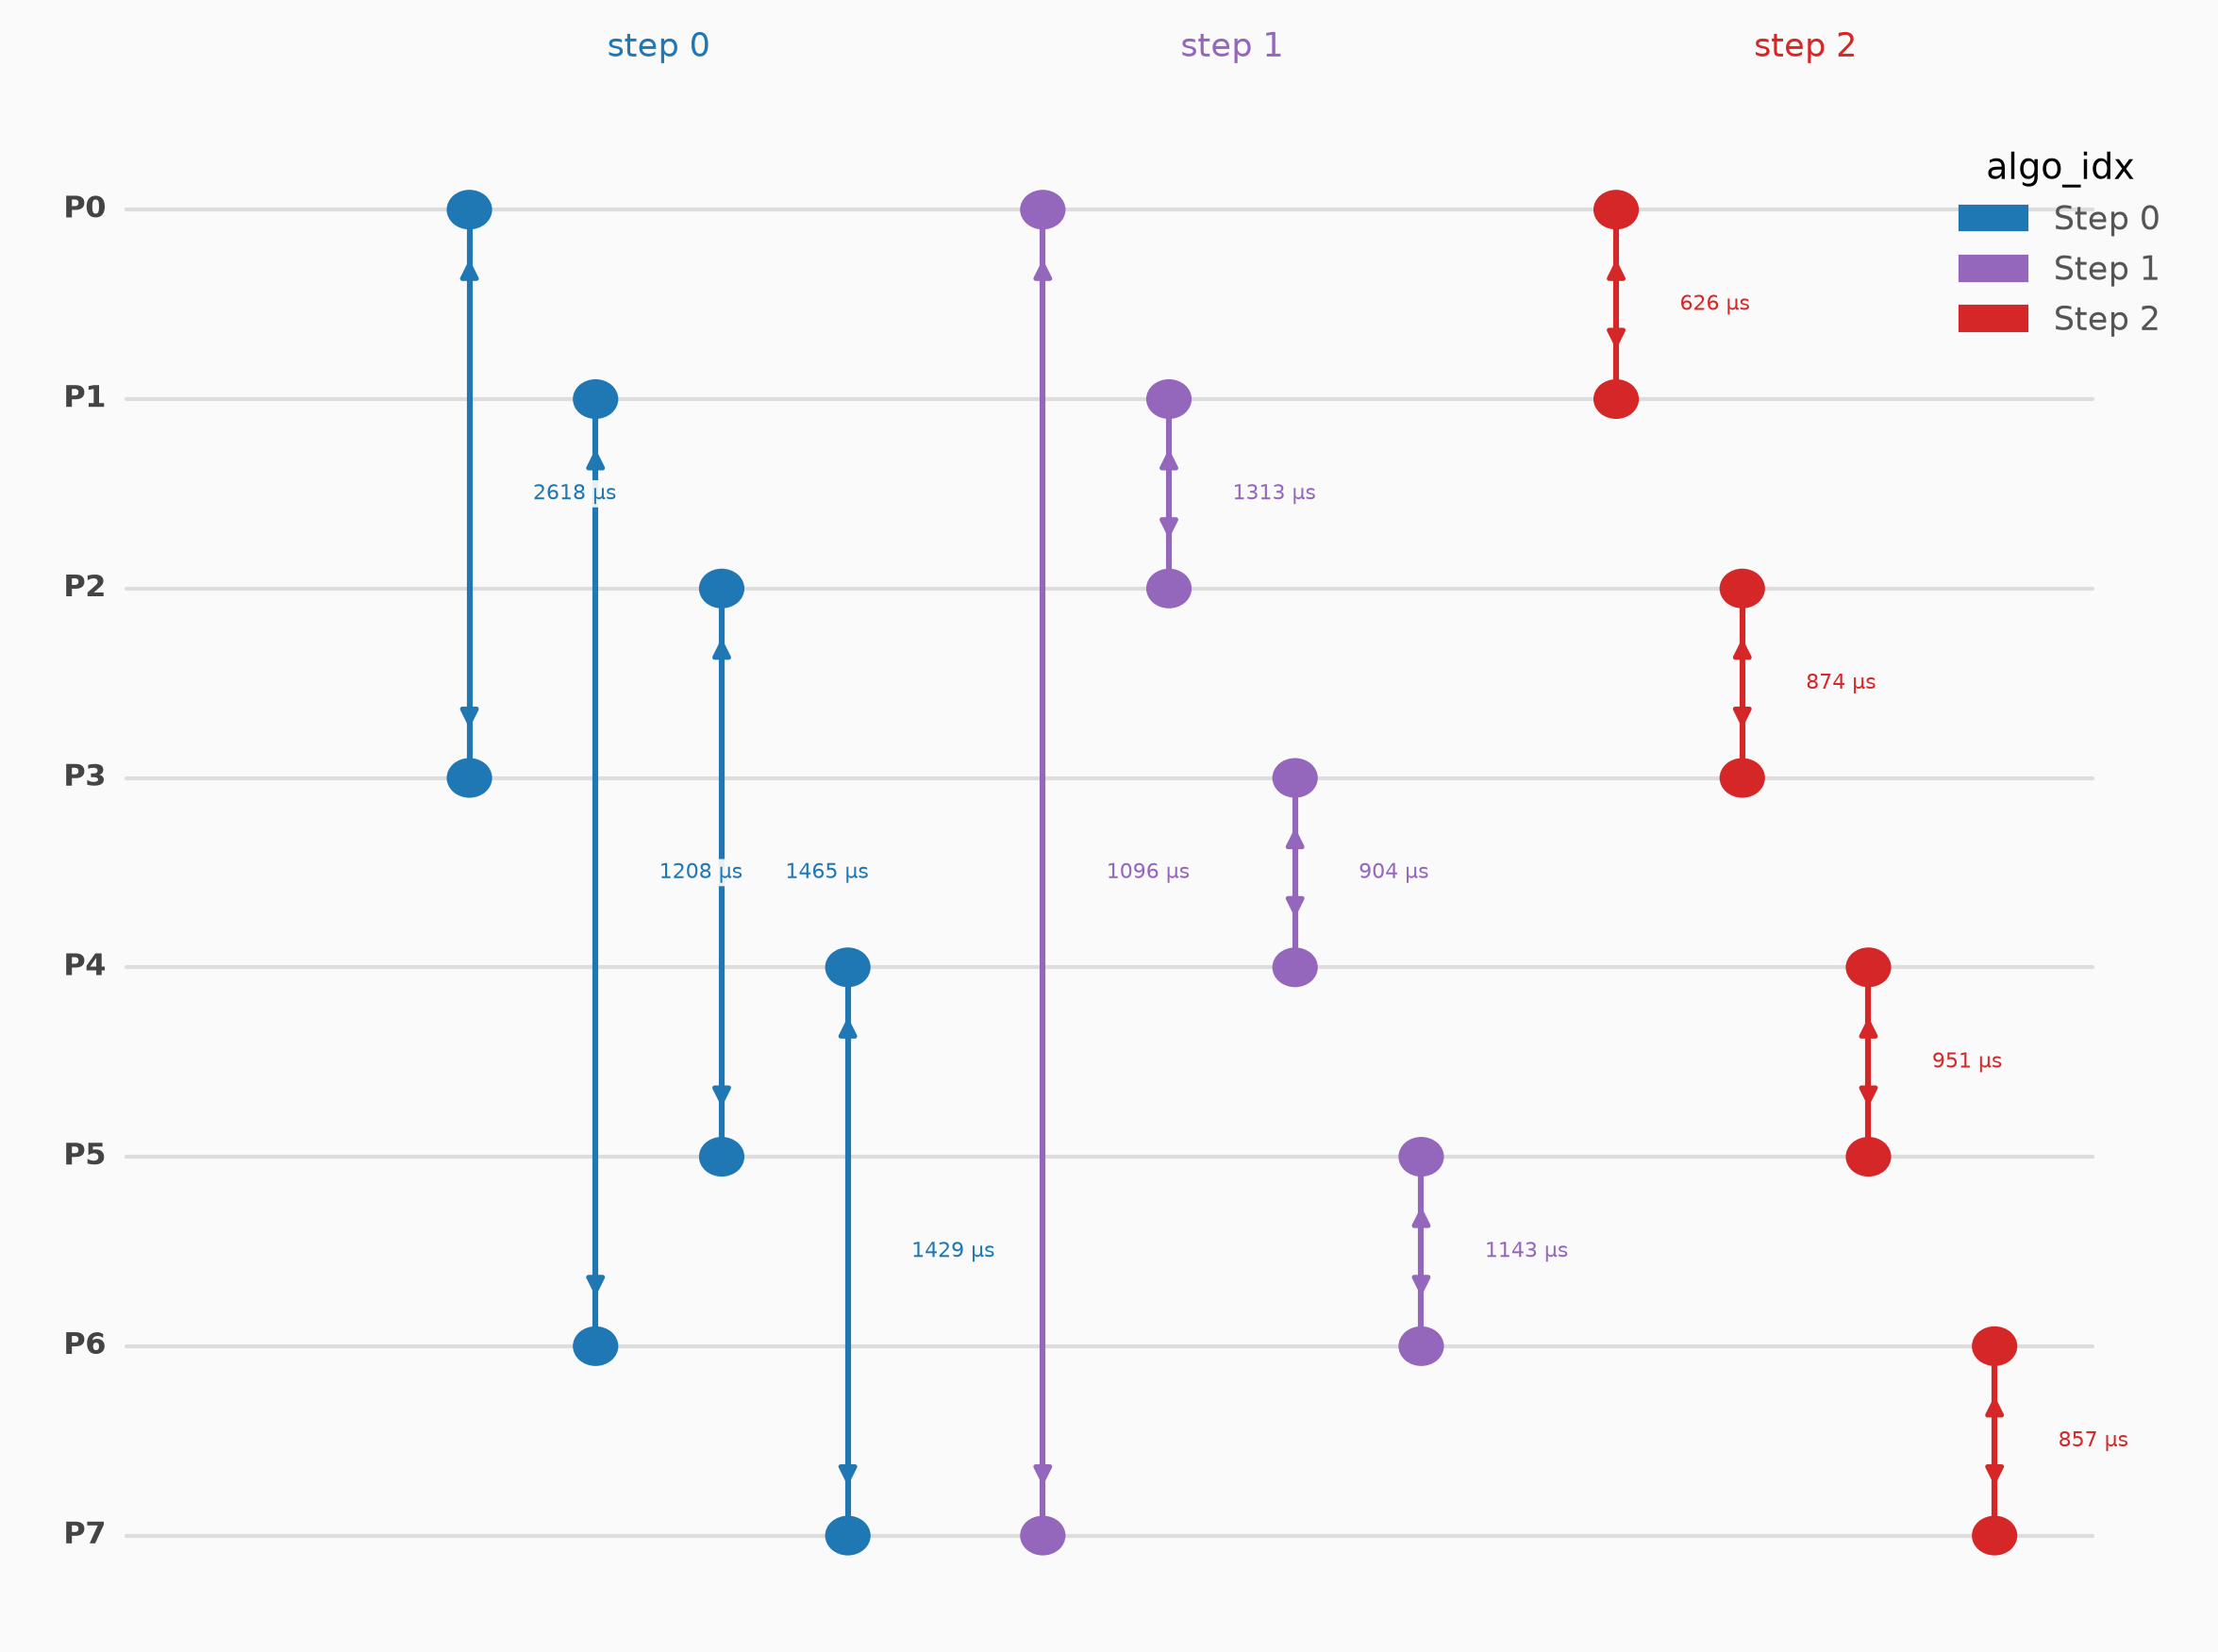
\includegraphics[width=0.62\linewidth]{collbench_ag_candle.png}
    \caption{Block-by-block \bine{} butterfly allgather, drawn by \texttt{butterfly.py} in candle mode. Each connector is the exchange between two ranks at one step, labelled with its duration.}
    \label{fig:sw-cb-candle}
  \end{subfigure}
  \caption{CollBench traces of two Collalgo collectives on $8$ ranks (four nodes with two GPUs each, CUDA-aware MPI), coloured by step.}
  \label{fig:sw-cb}
\end{figure}

% ---------------------------------------------------------------------------
\section{Collalgo}\label{sec:sw-collalgo}

Collalgo is a C11 library of \bine{} collectives over MPI, built with CMake and linked against CollBench, which it includes as a git submodule.
It is a workbench rather than a finished library: each collective is a direct transcription of an algorithm with MPI point-to-point calls, written to check a schedule and to look at its trace, and kept free of the buffer management and protocol details that \nccl{} adds.
The schedule helpers it contains (negabinary conversions, the remapping $\nu$ of the butterfly, the peer of a rank at a step) are the ones later ported to the \nccl{} fork.
What is worth describing is how the same source runs on host and on device buffers.

\paragraph{One source for host and device buffers.}
A collective does not take a flag telling it where its buffers are.
It asks: \texttt{CA\_is\_devptr} calls \texttt{cudaPointerGetAttributes} on the user's buffer and returns true for device and managed memory, and the answer is kept in a local \texttt{use\_cuda}.
Every operation that touches memory then goes through a small set of unified macros that take this flag:
\par\noindent\begin{minipage}{\linewidth}
\begin{lstlisting}[language=C, numbers=none]
int use_cuda = CA_is_devptr(sendbuff);
CA_UMALLOC(tmpbuff, bytes, use_cuda);            /* cudaMalloc | malloc */
CA_UMEMCPY(recvbuff, sendbuff, bytes, use_cuda); /* D2D copy | memcpy   */
...
CB_LRECV(rank, step, tmpbuff, count, datatype, peer, 0, comm);
local_reduce(tmpbuff, recvbuff, count, datatype, op, use_cuda);
...
CA_UFREE(tmpbuff, use_cuda);
\end{lstlisting}
\end{minipage}\par\smallskip
The communication itself needs no branch: device pointers are handed to MPI as they are, and a CUDA-aware MPI moves them directly between GPUs.
The only computation, the local reduction, dispatches to \texttt{MPI\_Reduce\_local} on the host or to a CUDA kernel on the device. The kernel is templated on the element type and on the operation (sum, product, minimum, maximum and the bitwise ones) and selected at run time from the \texttt{MPI\_Datatype} and \texttt{MPI\_Op} arguments, so the collective keeps the MPI signature.
CUDA is a build option (\texttt{-DCA\_CUDA=ON}): without it, \texttt{CA\_is\_devptr} returns $0$, the unified macros collapse to \texttt{malloc}, \texttt{memcpy} and \texttt{free}, no CUDA header is included, and the library builds on machines without the toolkit.
CUDA errors are checked by macros that print the failing call with its file and line and jump to the cleanup label of the collective, in the same style as the MPI and CollBench checks, so a failure on the device unwinds the same way as one on the host.
With this, the \bine{} schedules were first run on GPUs, with the trace of every message, before any \nccl{} code was written.

\paragraph{Benchmark.}
The \texttt{bench} executable runs every collective once on a known input, on host buffers (and, in CUDA builds, the broadcast and the reduce also on device buffers filled and checked by small kernels), checks the result against the expected one and, when the library is built with \texttt{-DCA\_PROFILE=ON}, writes the CollBench trace of each collective to \texttt{out/tree} or \texttt{out/butterfly}.

% ---------------------------------------------------------------------------
\section{fastest}\label{sec:sw-fastest}

fastest is a test and micro-benchmark framework for C code in which the tests are written in C and run, selected and analysed from Python.
It is a general-purpose tool, and unitccl is its main user in this thesis.
The motivation is that the code under test (here, \nccl{} with its CUDA and MPI dependencies) must be compiled and linked as C, while the orchestration around it (repeating runs, grouping tests, computing statistics, plotting, launching jobs) is much simpler to write in Python.

\paragraph{Test registration.}
A test is a C function that fills a \texttt{FASTEST\_TestOutput\_t}, and it is declared with one of the registration macros:
\begin{lstlisting}[language=C, numbers=none]
FASTEST_CUSTOMTEST_INLINE("standalone/tree/no_self_send", FASTEST_FAIL_ERROR, NULL, {
    out->exit_status = FASTEST_SUCCESS;
    /* ... on violation: out->exit_status = FASTEST_ERROR_ASSERT; */
});
\end{lstlisting}
Each macro defines the body as a static function and a second static function marked \texttt{\_\_attribute\_\_((constructor))}, which pushes the test into a global scheduler list when the library is loaded, before \texttt{main} or before the Python module finishes importing.
There is therefore no central list of tests to maintain: a test exists as soon as its translation unit is linked.
\texttt{FASTEST\_CUSTOMTEST} takes an existing function, \texttt{\_INLINE} an inline body, and \texttt{\_DINLINE} an inline body and an inline callback that runs after the test, for instance to print or post-process its output.
Test names are paths, so tests can be selected by prefix.

\paragraph{Outputs.}
The output of a test records its name, its flags, an exit status, allocation and deallocation counters, the wall-clock time measured by the scheduler around the test, and, for tests that run an inner loop of their own, the mean, the standard deviation and the number of the inner samples.
Flags and exit statuses are bitmaps.
The flags select the time unit to report, whether failures are errors, warnings or log entries, and whether memory is tracked. The exit statuses distinguish success and skip from failed assertions, unexpected states, resource, MPI and CUDA errors, so that a single integer tells why a test failed.

\paragraph{Python bindings.}
The bindings (\texttt{bindings/pybind.cpp}) are built per project with pybind11: the user's static library is linked with \texttt{--whole-archive}, so that every constructor is kept by the linker, and the module name is chosen at build time (\texttt{unitccl} for unitccl).
At import, the module exposes every registered test name as a constant in a \texttt{tests} submodule, plus \texttt{get\_tests}, \texttt{get\_subtests(prefix)}, \texttt{get\_test(name)} and \texttt{run\_test(name)}. C error codes are translated into the matching Python exceptions.
A typed stub file is generated next to the module for editor completion.

\paragraph{Runner.}
The \texttt{fastest} Python package wraps a backend module in a \texttt{Runner}.
Tests are grouped into \emph{pools}, built from a list of names or from a prefix, and \texttt{compare(*pools, n\_repeats)} runs every test of every pool $n$ times and returns a \texttt{CompareResult} with, for every test, the statistics across repeats (mean, standard deviation, minimum, maximum, median) and, when the backend provides them, the pooled statistics of the inner samples.
Results can be printed as a report, saved as JSON or CSV, and plotted with a builder-style \texttt{Plotter} that chooses the statistic to show (mean, median, \dots) and the axes.

% ---------------------------------------------------------------------------
\section{unitccl}\label{sec:sw-unitccl}

unitccl is the test and benchmark suite of the \nccl{} fork.
It contains the fork and fastest as git submodules, a C/CUDA part linked against the static \nccl{} library and compiled into a fastest backend, and a Python command-line tool, \texttt{unitccl}, that builds everything, runs the tests and the experiments locally or on Slurm, and plots the results.
\Cref{fig:sw-unitccl} shows how the parts fit together.

\begin{figure}[htbp]
  \centering
  \begin{tikzpicture}[x=1cm, y=1cm,
      box/.style={draw, rounded corners=2pt, minimum height=0.75cm, align=center,
                  font=\small, fill=white, inner xsep=5pt},
      arr/.style={-{Stealth[length=2mm]}, thick},
      lab/.style={font=\scriptsize, text=black!65}]
    \node[box, minimum width=12.4cm, fill=ch1!8] (cli) at (0,4.1)
      {\texttt{unitccl} CLI \quad {\scriptsize\texttt{build}\,·\,\texttt{standalone}\,·\,\texttt{scaling}\,·\,\texttt{nccltests}\,·\,\texttt{nsys}\,·\,\texttt{plot}}};
    \node[box, minimum width=12.4cm] (slurm) at (0,2.95)
      {Slurm via \texttt{submitit}: one job per rank count, sized from the configuration};
    \node[box] (fpy) at (-4.2,1.6) {fastest \texttt{Runner}\\[-1pt]\scriptsize pybind module \texttt{unitccl}};
    \node[box] (std) at (-5.2,0) {standalone tests\\[-1pt]\scriptsize schedule invariants};
    \node[box] (bt) at (-1.8,0) {scaling tests\\[-1pt]\scriptsize \texttt{popen(mpirun ...)}};
    \node[box] (ub) at (-1.8,-1.5) {\texttt{unitccl\_bench}\\[-1pt]\scriptsize MPI + \nccl{}, CUDA events};
    \node[box] (nt) at (2.9,0.8) {\texttt{nccl-tests}\\[-1pt]\scriptsize \texttt{*\_perf}, \texttt{-N} repeats};
    \node[box] (ns) at (5.45,0.8) {\texttt{nsys}\\[-1pt]\scriptsize profiles};
    \node[box, fill=ch0!8] (csv) at (2.9,-2.8)
      {\texttt{<p>\_ranks/<Coll>/<Coll>\_<PROTO>.csv}};
    \node[box] (plt) at (2.9,-4.0) {plots: ranks, size, heatmap, diff};
    \node[box, dashed] (fork) at (-5.2,-2.8) {\nccl{} fork\\[-1pt]\scriptsize \texttt{libnccl\_static.a}};
    \draw[arr] (cli) -- (slurm);
    \draw[arr] (slurm.south -| fpy) -- (fpy);
    \draw[arr] (slurm.south -| nt) -- (nt);
    \draw[arr] (slurm.south -| ns) -- (ns);
    \draw[arr] (fpy) -- (std);
    \draw[arr] (fpy) -- (bt);
    \draw[arr] (bt) -- (ub);
    \draw[arr, dashed] (std) -- node[lab, left] {links} (fork);
    \draw[arr, dashed] (ub) -- (fork);
    \draw[arr] (ub.south) |- (csv.west);
    \draw[arr] (nt) -- (csv.north -| nt);
    \draw[arr] (csv) -- (plt);
  \end{tikzpicture}
  \caption{Structure of unitccl. The standalone tests and the scaling tests are fastest tests compiled into the \texttt{unitccl} Python module. The scaling tests and \texttt{nccl-tests} write the same CSV schema, so the plots do not depend on which benchmark produced the data.}
  \label{fig:sw-unitccl}
\end{figure}

\paragraph{Standalone tests.}
The standalone tests call the schedule generators of the fork directly on the host, without GPUs or MPI: \texttt{ncclGetBineTree} for the tree, and \texttt{ncclGetBineButterflyDdbl} and \texttt{ncclGetBineButterflyDhlv} for the distance-doubling and distance-halving butterflies, with $7$, $7$ and $8$ tests respectively.
Each test checks one of the invariants of \cref{sec:tree-testing,sec:bfly-testing}, the distance-halving ones including the reversal of the distance-doubling table, the non-increasing distance and the circular windows, over every power of two up to $2^{12}$ ranks and, for the tree, every root, and reports the first violation it finds with the values of $p$, root, rank and step.
Because they need neither GPUs nor a network, they run in seconds on a laptop and were run after every change to the schedule code.

\paragraph{Scaling with \texttt{unitccl\_bench}.}
\texttt{unitccl\_bench} is a small MPI and \nccl{} program that runs one collective of a given size with one MPI rank per GPU.
The \nccl{} communicator is created from a unique identifier broadcast with MPI.
Before every iteration the ranks synchronise with an \texttt{MPI\_Barrier}, so that each iteration starts from aligned ranks, and the collective is timed on the GPU with CUDA events.
The time of an iteration is the maximum over the ranks (an \texttt{MPI\_Reduce} with \texttt{MPI\_MAX}), because a collective is finished only when its slowest rank is, and rank $0$ reports the median, mean, standard deviation and minimum of these values over the measured iterations ($40$ after $10$ warmup iterations by default).
The send buffer of rank $r$ holds $(r+1)\,i$ at index $i$, and the receive buffer is filled with NaNs before every iteration, so that the optional correctness check on the first iteration detects both wrong and missing elements.
The algorithm is selected with \texttt{NCCL\_ALGO}, and the \bine{} variant and buffer-management strategy with the environment variables of the fork.

On the fastest side, a scaling test is one (collective, algorithm, size) triple, registered by a macro that expands to the six sizes from 1\,kB to 64\,MB:
\begin{lstlisting}[language=C, numbers=none]
DEFINE_TEST_1KB_64MB("AllGather", "BINE")
DEFINE_TEST_1KB_64MB("AllGather", "RING")
DEFINE_TEST_1KB_64MB("AllGather", "PAT")
\end{lstlisting}
Each test launches \texttt{unitccl\_bench} with \texttt{mpirun} through \texttt{popen}, parses the statistics it prints into its fastest output, and sets the exit status from the worst status of any rank.
Running the benchmark as a separate process keeps every test in a fresh \nccl{} environment, which is required because \nccl{} reads most of its configuration from the environment only once, at initialisation.

\paragraph{Scaling with \texttt{nccl-tests}.}
The \texttt{nccltests} subcommand runs the same sweep with NVIDIA's \texttt{nccl-tests} instead, as an independent check of \texttt{unitccl\_bench}.
\texttt{nccl-tests} times its iterations back to back with no barrier in between and reports their mean, so it measures a pipelined throughput rather than the latency of an isolated collective. Repeating each size $R$ times (\texttt{-N}) gives $R$ samples per point.
Its sizes are converted so that both tools refer to the same per-rank buffer, and its results are written to the same CSV files, all reported datata points come from the \texttt{nccl-tests} branch.

\paragraph{Sweeps on Slurm.}
A sweep is described by the collectives, algorithms, protocols and rank counts to measure.
For each rank count, the CLI submits one Slurm job, sized from the configuration of the machine (GPUs per node, partition, account and modules, stored in a per-user JSON file with presets for MeluXina and Leonardo), through \texttt{submitit}, and follows the jobs in a live terminal dashboard from which they can be cancelled.
For \nccl{}'s native \pat{}, which only runs with one GPU per node, the jobs are automatically placed one rank per node, and their results are merged into the same files as the others.
When the algorithm is \bine{}, the sweep crosses the variants (tree, butterfly, \pat{}) with the buffer-management strategies (send, permute, block-by-block, double send) of \cref{ch:butterfly,ch:pat}, skipping the combinations that do not exist (the tree has a single strategy, and the tree and \bine{}-\pat{} have no \texttt{LL} implementation).

\paragraph{Results and profiling.}
The results are stored as one CSV file per collective and protocol under a directory per rank count, with one row per algorithm, configuration and size holding the statistics of that point (mean, median, standard deviation, minimum and maximum, plus the per-iteration statistics of \texttt{unitccl\_bench}).
The \texttt{plot} subcommand produces the four kinds of plots used in \cref{ch:tree,ch:butterfly,ch:pat,ch:treeallreduce}: time against the number of ranks for each size, time against size for each number of ranks, the relative difference between two algorithms, and the heatmaps of the fastest algorithm at each point.
Finally, the \texttt{nsys} subcommand runs the benchmark under Nsight Systems, exports the kernel, memory-copy and NVTX summaries to CSV and compares the kernel time of \bine{} and of the ring, to tell the time spent in the kernels apart from the time spent around them.

\chapter{Conclusion}\label{ch:conclusion}

This thesis implemented the \bine{} algorithms~\cite{desensi2025bine} inside \nccl{}, as four components: a tree-based broadcast and reduce (\cref{ch:tree}), a butterfly allgather and reduce-scatter (\cref{ch:butterfly}), the same allgather rebuilt on the \pat{} machinery (\cref{ch:pat}), and a tree-based allreduce that composes the same \bine{} tree into a single fused reduce-and-broadcast kernel (\cref{ch:treeallreduce}).
Across the four, the experiments of \cref{sec:tree-results,sec:bfly-results,sec:pat-exp,sec:tar-results} draw a consistent picture of where the \bine{} structure pays for itself inside \nccl{} and where it does not.

\paragraph{Broadcast and reduce.}
The tree of \cref{ch:tree} wins in the band between the two regimes in which the ring is already good: below it, the ring with \texttt{LL} is latency-optimised and hard to beat (\cref{sec:tree-ll}). Above it, with \texttt{SIMPLE} the ring becomes bandwidth-bound and its optimal bandwidth term takes over (\cref{sec:bg-ring-vs-tree}).
In between, from a few kB to a few MB and from $8$ ranks on, the logarithmic number of steps of the tree dominates, with speedups of $3.4$--$6.5\times$ over the ring at $128$ ranks (\cref{sec:tree-results}).

\paragraph{Allgather and reduce-scatter.}
The butterfly of \cref{ch:butterfly} only pays off in \emph{pos} mode, below the $n_cS$ crossover of \cref{eq:bfly-pos}, where a channel owns whole blocks and send and double send move a window as one contiguous, full-chunk transfer. In \emph{slice} mode, which is where every size above a few hundred kB falls, every strategy degrades to the calls of block-by-block while keeping its own extra cost, so none of send, permute or double send is ever worth it there (\cref{sec:bfly-res-modes}).
The measurements start at 1\,kB, the smallest size exercised, where \bine{} already grows with $p$ by a constant instead of doubling like the ring (\cref{sec:bfly-res-ring}). Nothing in the mechanism changes below that point, so the same gap, or a larger one, is expected for yet smaller blocks, only outside the range that was measured here.
Rebuilding the same schedule on the \pat{} machinery (\cref{ch:pat}) removes the dependence of the transfers on the data layout: all four strategies become equivalent, and block-by-block, the simplest, is the best one (\cref{sec:pat-res-modes}).
It does not, however, make the allgather faster in the configuration used throughout this thesis, four ranks per node: from $16$ ranks on \bine{}-\pat{} is $3$--$14\,\%$ slower than the butterfly kernels for large blocks and up to $2.2\times$ slower for small ones, and it is never the fastest algorithm once the ring may use \texttt{LL} (\cref{sec:pat-res-bfly,sec:pat-res-ring}).
It is competitive, and in one regime already ahead, only where the comparison is with \pat{} on its own terms, one rank per node, the only configuration the native \nccl{} \pat{} allgather supports (\cref{sec:pat-res-native}): there \bine{}-\pat{} is $1.55$--$1.74\times$ faster than the ring with \texttt{SIMPLE} and still ahead of the ring with \texttt{LL} at 16\,kB from $8$ ranks on.
For small blocks the native \pat{} remains faster, thanks to a parallel factor and a fused receive-and-forward that \bine{}-\pat{} does not yet have, and the gap widens with $p$ over the tested range ($1.14\times$ at $4$ ranks to $1.47\times$ at $16$). This is a cost of the kernel, not of the schedule, so it is not expected to close with scale alone.
For blocks of 1\,MB or more, instead, \bine{}-\pat{} is already $5$--$8\,\%$ \emph{faster} than the native \pat{} at the largest rank count tested, $16$, which the text attributes to the shorter average inter-node distance of the \bine{} schedule -- a structural property of the schedule, not an artefact of this range, so the advantage is expected to hold, and plausibly grow, at the larger rank counts this thesis did not have the allocation to reach.

\paragraph{Allreduce.}
The tree-based allreduce of \cref{ch:treeallreduce} roots a \bine{} tree differently on each channel and runs it as a single fused reduce-and-broadcast kernel.
The idea does not come from the reduce-scatter-plus-allgather composition of \cref{ch:butterfly}, whose windows halve and double at every step, but from the other allreduce of the \bine{} paper, the recursive doubling that exchanges the whole vector at every step with no such growth (Sec.~4.5 of~\cite{desensi2025bine}, \cref{sec:tar-motivation}): the multi-root tree can be read as that same pattern restricted to $\min(p,\mathit{nchannels})$ simultaneous instances, one per channel, to match the number of channels \nccl{} actually runs, instead of one per rank (\cref{sec:tar-schedule}).
Of the four components, it has the best range: against the reduce-scatter-plus-allgather allreduce of the \bine{} butterfly, which does grow and shrink its windows, the tree is still the fastest algorithm at 1\,MB on every scale and at 4\,MB from $32$ ranks on, and the gap is largest exactly there: the butterfly allreduce is $1.3$--$3.4\times$ slower at 1\,MB and $1.6$--$2.5\times$ slower at 4\,MB, growing with the number of ranks (\cref{fig:tar-heatmap-simple}).
It also matches or beats the native \nccl{} tree up to 1\,MB on almost every scale (\cref{sec:tar-results}).

\section{Future work}
Several directions follow directly from the limits above.

The standalone reduce and broadcast of \cref{ch:tree} process one child at a time in program order, a fresh single-peer \texttt{Primitives} object per level (\cref{sec:tree-collectives}), with the reduce in particular \emph{step-outer} (\cref{fig:bine-step-outer}).
This is a logical order, not a literal one: a send only blocks once the FIFO behind it is full, so consecutive levels already overlap in practice up to its depth, as \cref{sec:tree-collectives} notes for the broadcast.
A version with a single, wide-fan \texttt{Primitives} object per kernel, the same change that lets the fused allreduce of \cref{ch:treeallreduce} overlap its levels explicitly, was prototyped for both collectives. The preliminary runs showed an improvement only past the point where the ring already overtakes the tree (\cref{sec:tree-results}), i.e., outside the range where the tree is the better choice anyway.
Whether it helps inside that range is not established: a conclusive comparison would have to sweep the number of channels, the root, the message size, the number of ranks and the reduction operation against the existing kernels, a long sweep for the reduce in particular.
It is this evaluation, not the kernel change, that is left for future work.

The allgather rebuilt on the \pat{} machinery (\cref{ch:pat}) is also left short of what the machinery supports: it runs with a parallel factor of $1$, a single group of workers executing every piece in order, and without the fused receive-and-forward that keeps a piece in its slot and forwards it from there (\cref{sec:pat-kernel}).
Both are already present in the native \pat{} allgather and are what \cref{sec:pat-res-bfly,sec:pat-res-native} point to as the cause of the remaining gap at small blocks. Nothing in the \bine{} schedule ties its operations to a single worker group, so raising the parallel factor and fusing the forward are natural next steps, not a redesign.

A further direction follows from the comparisons throughout this thesis, which are against \nccl{}'s own ring and double binary tree, never against a plain, non-\bine{} binomial tree under the same kernels and the same system.
Implementing the classic distance-halving binomial tree (\cref{sec:bg-bine}) as a fourth \nccl{} algorithm, alongside \bine{}, would isolate the gain that comes specifically from \bine{}'s shorter average distance between communicating ranks from the gain of using a pipelined tree at all, which the comparisons of this thesis do not separate.

The tree-based allreduce also leaves two things on the table.
The multi-root tree uses a single \bine{} tree per channel, whose root has $\log_2p$ children and therefore a bandwidth term that grows with $p$. Combining two complementary trees, as \nccl{} does with its double binary tree (\cref{sec:bg-double-tree}), would remove this dependence for large vectors, which \cref{sec:tar-motivation} already identifies as the chapter's main limitation, and is left there as future work.
The second tree is not the obstacle, since the construction of \cref{sec:bg-bine} already gives one for any root. The obstacle is the load-balancing step that makes \nccl{}'s own double binary tree work, which books only half the inter-node bandwidth at the two boundary GPUs because every rank is a leaf with a fixed, small arity in one tree and an internal node in the other (\cref{sec:nccl-graph}).
A \bine{} tree does not have a fixed arity, so finding an equally effective balancing rule for it, one that holds across channels, roots and ranks rather than for a single fixed pair of trees, is the biggest hurdle to a \bine{} double tree, not the tree itself.

And the root of each channel is currently chosen once, by the bit-reversal permutation of \cref{sec:tar-schedule}, which only spreads the $\min(p,\mathit{nchannels})$ roots apart. A schedule that also balances the fan-out and the link load across channels, rather than only their position, could close part of the remaining gap with the native tree on the scales where it still wins.
The choice of graph is itself worth revisiting: among the alternatives tried, the default ring graph of \cref{sec:nccl-graph} proved more consistent across topologies and allocations, and its permutation minimises the hop-to-hop distance around the whole cycle, wrap-around edge included, which only approximates minimising the modular distance that \bine{} actually cares about.
A search built around \bine{}'s own edges, the specific pairs its tree and butterfly connect at each step, rather than the ring's adjacent pairs, might do better than this coincidence, though whether it would generalise as consistently as the ring graph does across topologies and allocations is itself an open question.

Last, the \emph{pos}/\emph{slice} split of the butterfly (\cref{sec:bfly-pos}) exists only because a window doubles, or halves, in size at every step of the allgather and the reduce-scatter, while the partition of \nccl{} is fixed across channels before the kernel starts (\cref{sec:nccl-cbd}).
\Cref{ch:pat} already tried the kernel-side answer, aggregating the steps on the \pat{} machinery instead of repartitioning, and it removes the dependence on the data layout without making the allgather faster (\cref{sec:pat-res-bfly}).
The partition itself is therefore the lever left: a channel repartitioner that reassigns the work between channels at run time, as the window grows or shrinks from one step to the next, would let the contiguous, full-chunk transfers of \emph{pos} mode apply past the few hundred kB where they give out today, at the cost of changes to the continuous byte distribution of \nccl{} (\cref{sec:nccl-cbd}) that go well beyond the kernels this thesis touched.


% ---------------------------------------------------------------------------
% Back matter
% ---------------------------------------------------------------------------
\appendix
% \chapter{Additional Material}\label{app:a}

\todo{Extra plots, full tables, code excerpts.}


\backmatter
% \nocite{*}   % removed: it would list uncited entries (e.g., LEONARDO)
\printbibliography[heading=bibintoc]

\begin{acknowledgments}
I would like to thank my advisor, Prof.\ Daniele De Sensi, and the whole HLC Lab, for their guidance throughout this thesis, for the trust they placed in me in giving me access to the infrastructure it required, and for the opportunities they offered me beyond it.

\begin{center}
  \IfFileExists{assets/icons/hlc.png}{%
    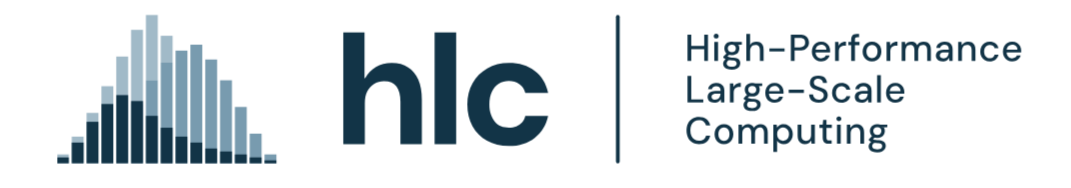
\includegraphics[height=1.5cm]{assets/icons/hlc.png}%
  }{\todo{Place the HLC Lab logo in assets/icons/hlc.png}}%
\end{center}

I would also like to thank my family, for their constant support, and my friends, who have been by my side throughout this journey.
In particular, I would like to thank Federico Sampalmieri, Marco, Martina Monetti, Martina Giacalone, Tommaso, Daniele, Alessandro, Massimo and Lorenzo Cipolletti, with whom I shared the university benches and the countless hours of study that brought me to this moment,
Elia, Leonardo, Jacopo, Iva, Matteo, Mariam, Lorenzo Piarulli and Saverio Pasqualoni, with whom I shared an eventful trip to Chicago for SC26 and who gave me invaluable advice for my academic career,
and, last but not least, Flavio, Gabriele and Federico Governatori, with whom I share a passion for motorsport that keeps taking us all over Italy.

    \newpage{}

The experiments presented in this thesis were performed on two supercomputers, and we thank the centres that made them available.

\definecolor{meluxinaRed}{HTML}{E30613}
\definecolor{meluxinaBlue}{HTML}{0099FF}

\paragraph{MeluXina.}
Some of the experiments were performed on the Luxembourg national supercomputer MeluXina.
We gratefully acknowledge the LuxProvide teams for their expert support.

\begin{center}
  \IfFileExists{assets/icons/meluxina.png}{%
    
\includegraphics[height=2.5cm]{assets/icons/meluxina.png}%
  }{\todo{Place the MeluXina logo in assets/icons/meluxina.png}}%
  \hspace{2cm}%
  \IfFileExists{assets/icons/luxprovide.png}{%
    
\includegraphics[height=2.5cm]{assets/icons/luxprovide.png}%
  }{\todo{Place the LuxProvide logo in assets/icons/luxprovide.png}}\\[6pt]
  {\color{meluxinaRed}\rule{0.2\linewidth}{1pt}}{\color{meluxinaBlue}\rule{0.2\linewidth}{1pt}}
\end{center}

\paragraph{Leonardo.}
We acknowledge ISCRA for awarding this project access to the Leonardo supercomputer, owned by the EuroHPC Joint Undertaking, hosted by CINECA (Italy).
The architecture of Leonardo and of its GPU-accelerated partition is described in~\cite{turisini2024leonardo}.
\begin{center}
  \IfFileExists{assets/icons/leonardo.png}{%
    
\includegraphics[height=2.5cm]{assets/icons/leonardo.png}%
  }{\todo{Place the Leonardo logo in assets/icons/leonardo.png}}%
\end{center}

\end{acknowledgments}


\end{document}
